% !TEX program = xelatex
% !TEX encoding = UTF-8  (utf8)

%%%%% basic settings
% !TEX root = ../0-main-LN.tex

\documentclass[a4paper, punct, adobefonts, UTF8]{ctexbook}
%openany 可以在任意页开始新的一章,否则只能在奇数页开始
%punct 对中文标点进行调整
%noindent 段首不缩进

%\documentclass[a4paper, openany, punct, adobefonts, UTF8]{ctexbook}%{ctexart}
% \documentclass[a4paper, openany, UTF8, punct, adobefonts]{book}
% \documentclass[a4paper, openany, twocolumn, UTF8, punct,adobefonts]{ctexbook}%{ctexart}
% \documentclass[a4paper,twocolumn,12pt]{article}

%\usepackage[keeplastbox]{flushend}		%使双栏文本的底端对齐
%\usepackage{cuted}			%支持双栏文本

%%%%% page layout
% \usepackage[top=1in, bottom=1in, left=1.25in, right=1in]{geometry}
% \usepackage[top=1in, bottom=1in, left=1in, right=1in]{geometry}
% \usepackage[left={3cm},right={3cm},marginparwidth={2cm},
% marginparsep={1em},vmargin={2cm},]{geometry}
%\usepackage[left={2cm},right={4cm},marginparwidth={3cm},
%	marginparsep={1em},vmargin={2cm}]{geometry}
\usepackage[left={2cm},right={5cm},marginparwidth={4cm},
	marginparsep={1em},vmargin={2cm}]{geometry}
% \usepackage[top=.6in, bottom=.6in, left=1in, right=1in]{geometry}
%\setlength{\parindent}{0pt}

%%%%% margin note
\usepackage{marginnote}

%%%%% TOC with hyperlinks
\usepackage[colorlinks,linkcolor=blue!80!yellow,
	anchorcolor=red,citecolor=green]{hyperref}

%%%%% math settings
\usepackage{amsmath}		%数学环境,align, align*
\usepackage{amsfonts}		%数学字体,mathbb
\usepackage{amssymb}		%数学公式
%\usepackage{amsthm}			%已包含在amsmath中
%\usepackage{mathrsfs}		%数学花体
\usepackage{extarrows}		%\xlongequal
\usepackage{bm}				%bm

\usepackage{tikz}
%\usetikzlibrary{arrows,snakes,backgrounds,petri}

%\usepackage{color}
\usepackage{xcolor}

\usepackage{graphics}
\usepackage{graphicx}		%definecolor, colorbox, fcolorbox
\usepackage{wrapfig}		%文字环绕的图片

\usepackage{framed}			%support shaded environment

\usepackage[justification=centering]{caption} %全局图片标题居中
\captionsetup[figure]{font={small,it},labelfont={up}}
\usepackage{subcaption}
%\usepackage[labelfont=bf,textfont=normalfont,singlelinecheck=off,%justification=raggedright]{subcaption}

\usepackage{ulem}			%各种下划线:uline, uuline, uwave, sout, xout
%\usepackage{enumerate}
%\usepackage{esint}			%any type of integral symbol
% \usepackage{tabularx}
% \usepackage{multirow}
% \usepackage{verbatim}
% \usepackage{listings}
\usepackage{polynom}		%多项式的竖式带余除法
%\usepackage{overpic}		%允许在图片上写文字
%\usepackage{wrapfig}		%支持插入文字环绕的图片
\usepackage{booktabs}		%粗的表格横线

\usepackage{tcolorbox} 		%各种自定义的盒子
\tcbuselibrary{skins, breakable, theorems}

%%%%% extended list environments
\usepackage{paralist}		%控制段间距等

%%%%% Chinese Font Config
%-----------------------xeCJK下设置中文字体------------------------------%
%常用字体
\setCJKfamilyfont{song}{Adobe Song Std}				%Adobe宋 \song
\newcommand{\song}{\CJKfamily{song}}                
      
\setCJKfamilyfont{fsong}{Adobe Fangsong Std}			%adobe仿宋 \fsong
\newcommand{\fsong}{\CJKfamily{fsong}}

\setCJKfamilyfont{kai}{Adobe Kaiti Std}				%Adobe楷体 \kaiti
\newcommand{\kaiti}{\CJKfamily{kai}}

\setCJKfamilyfont{hei}{Adobe Heiti Std}				%Adobe黑体 \heiti
\renewcommand{\heiti}{\CJKfamily{hei}}

\setCJKfamilyfont{hwzs}{STZhongsong}				%华文中宋 \hwzs
\newcommand{\hwzs}{\CJKfamily{hwzs}}

\setCJKfamilyfont{yh}{Microsoft YaHei}				%微软雅黑 \msyh
\newcommand{\msyh}{\CJKfamily{yh}}

%其他字体
\setCJKfamilyfont{hwfs}{STFangsong}				%华文仿宋  hwfs
\newcommand{\hwfs}{\CJKfamily{hwfs}}

\setCJKfamilyfont{hwxh}{STXihei}					%华文细黑  hwxh
\newcommand{\hwxh}{\CJKfamily{hwxh}}

\setCJKfamilyfont{hwl}{STLiti}						%华文隶书  hwl
\newcommand{\hwls}{\CJKfamily{hwl}}

\setCJKfamilyfont{hwxw}{STXinwei}					%华文新魏  hwxw
\newcommand{\hwxw}{\CJKfamily{hwxw}}

\setCJKfamilyfont{hwxk}{STXingkai}					%华文行楷  hwxk
\newcommand{\hwxk}{\CJKfamily{hwxk}}

\setCJKfamilyfont{hwhp}{STHupo}					%华文琥珀   hwhp
\newcommand{\hwhp}{\CJKfamily{hwhp}}

\setCJKfamilyfont{wawati}{Wawati SC}				%娃娃体 wawati
\newcommand{\wawati}{\CJKfamily{wawati}}

%------------------------------设置字体大小------------------------%
\newcommand{\chuhao}{\fontsize{42pt}{\baselineskip}\selectfont}     %初号
\newcommand{\xiaochuhao}{\fontsize{36pt}{\baselineskip}\selectfont} %小初号
\newcommand{\yihao}{\fontsize{28pt}{\baselineskip}\selectfont}      %一号
\newcommand{\erhao}{\fontsize{21pt}{\baselineskip}\selectfont}      %二号
\newcommand{\xiaoerhao}{\fontsize{18pt}{\baselineskip}\selectfont}  %小二号
\newcommand{\sanhao}{\fontsize{15.75pt}{\baselineskip}\selectfont}  %三号
\newcommand{\sihao}{\fontsize{14pt}{\baselineskip}\selectfont}%     四号
\newcommand{\xiaosihao}{\fontsize{12pt}{\baselineskip}\selectfont}  %小四号
\newcommand{\wuhao}{\fontsize{10.5pt}{\baselineskip}\selectfont}    %五号
\newcommand{\xiaowuhao}{\fontsize{9pt}{\baselineskip}\selectfont}   %小五号
\newcommand{\liuhao}{\fontsize{7.875pt}{\baselineskip}\selectfont}  %六号
\newcommand{\qihao}{\fontsize{5.25pt}{\baselineskip}\selectfont}    %七号

%%%%% head and foot setting
 \usepackage{fancyhdr}
 \pagestyle{fancyplain}
 %\renewcommand{\chaptermark}[1]{\markboth{\chaptername .\;\ #1}{}}
 %\renewcommand{\chaptermark}[1]{\markboth{\chaptername .\;\ #1}{}}
 %\renewcommand{\sectionmark}[1]{\markright{\thesection \ #1}{}}
 \fancyhf{}
 \fancyhead[RE,LO]{\fangsong\leftmark}
 \fancyhead[LE,RO]{\fangsong\rightmark}
 \fancyhead[CE,CO]{} %
 \fancyfoot[LE,RO]{\color{gray} AM-NUDT-2018-S3,
 \number\day-\number\month-\number\year}
 \fancyfoot[LO,RE]{\fangsong -\,\thepage\,-}
% \renewcommand{\headrulewidth}{2pt}
% \renewcommand{\footrulewidth}{1pt}
% \renewcommand{\headrulewidth}{0pt}
% \usepackage[CJKbookmarks=true,bookmarksnumbered,bookmarksopen,
% colorlinks,linkcolor=blue,anchorcolor=blue,citecolor=green,dvipdfm]{hyperref}
% \excludecomment{student}
% \includecomment{teacher}
\clearpage{\pagestyle{empty}\cleardoublepage}

%%%%% page watermark
\usepackage[all, scale=10, color=purple!5,
angle=70,contents=NUDT-2018-S3]{background}

%%%%% background color of the page
% \definecolor{myback}{RGB}{204,232,207}
% \pagecolor{yellow!10!white}
% \renewcommand{\baselinestretch}{1.25}

%%%%% if-then control
\usepackage{ifthen}
%%%%% content visibility control
%用\newif来定义一个判断变量\ifabc,初始值一律为false,
%则除了\ifabc外,还自动生成两个控制序列\abctrue和\abcfalse;
%用\abctrue来设置为true,还可以用\abcfalse来设置为false
%\ifabc和\fi之间的内容由\ifabc来控制是否出现
\newif\ifvisible
\newif\ifanswer  % if the answer of homework
\newif\ifhint % if the hint to exercise
\newif\ifnottest % if its a test
% \visibletrue
% \visiblefalse

%%%%% my macros
%===============macros====================
\def\ds{\displaystyle}
% \def\fin{\hfill$\Box$}
\def\fin{\hfill{\color{green!50!black}$\blacksquare$}}
\def\bs{\bigskip}
\def\b{\color{blue!80!yellow}}
\def\bb{\bf\color{blue}}
\def\e{\ensuremath{\varepsilon}}

\newcommand{\ba}[1]{\alert{\bf #1}}
\providecommand{\mbb}[1]{\ensuremath{\mathbb{{#1}}}}
\providecommand{\mr}[1]{\ensuremath{\mathrm{{#1}}}}


\newcommand{\limn}{\ensuremath{\lim\limits_{n\to\infty}}}
\newcommand*{\limx}[1]{\ensuremath{\lim\limits_{x\to{#1}}}}
\newcommand*{\limdx}{\ensuremath{\lim\limits_{\Delta x\to 0}}}
\providecommand{\llim}[1]{\ensuremath{\lim\limits_{#1}}}

\newcommand{\sumn}[1][1]{\ensuremath{\sum\limits_{n=#1}^{\infty}}}
\providecommand{\sumk}[1]{\ensuremath{\sum\limits_{k={#1}}^n}}
\providecommand{\suml}{\ensuremath{\sum\limits}}

\newcommand*{\df}[2]{\displaystyle\frac{\,{#1}\,}{\,{#2}\,}}
\newcommand*{\dx}{\Delta x}
\renewcommand{\d}{\mathrm{d}}
\newcommand*{\p}{\ensuremath{\partial}}

\newcommand{\dint}{\ensuremath{\displaystyle\int}}

\newcommand{\ps}[1]{$^{[\mbox{\kaiti\footnotesize 注}]}$
\marginpar{\kaiti\small\color{blue} {注:}#1}}

%define tab of .25 textwidth and can auto strech
%\tab{the word}\tab{another word}\tab{3rd one}
\newlength{\tabcont}
\newcommand{\tab}[1]{%
	\settowidth{\tabcont}{#1}%
	\ifthenelse{\lengthtest{\tabcont < .25\linewidth}}%
	{\makebox[.25\linewidth][l]{#1}\ignorespaces}%
	%{\makebox[.5\linewidth][l]{\color{red} #1}\ignorespaces}%
	{\makebox[.5\linewidth][l]{#1}\ignorespaces}%
}%

%set fontsize with number of points
% \newcommand{\fs}[1]{\fontsize{#1 pt}{5pt}\selectfont}

\newtcolorbox{thx}{colframe=blue!40!black,colback=white,breakable}

\newtcolorbox{ext}{colframe=green!60!black,colback=green!20!white,breakable}

\definecolor{shadecolor}{rgb}{0.9,0.9,0.9}

\renewcommand{\thefigure}{\thechapter.\arabic{figure}}

\begin{document}

%%%%% if answer is visible
\answertrue
%%%%% if hint is visible
\hinttrue
%%%%% if it is a test
\nottesttrue

\ifnottest
	%%%%% level of TOC
	\setcounter{tocdepth}{3}%控制目录显示的层级
	\tableofcontents
\fi

%%%%% background color of the document
%\pagecolor{yellow!10!white}
%\pagecolor{gray!10!white}

\thispagestyle{empty}

%%%%% let the split from list to para compact
\let\itemize\compactitem 
\let\enditemize\endcompactitem 
\let\enumerate\compactenum
\let\endenumerate\endcompactenum 
\let\description\compactdesc 
\let\enddescription\endcompactdesc
\setlength{\pltopsep}{0pt}
%%%%% keep tight between math formula and its contex
\setlength\abovedisplayskip{0pt}
\setlength\belowdisplayskip{0pt}

\ifnottest
	\bs\bs

	\hrule

	\bs\bs 
	{\bf 说明}

	{\kaishu 本讲义主要作为教师讲课和学生课后复习的参考,
	与相关教材在基本内容上一致,但在知识讲授的次序上无严格关联。}

	\bs

	{\kaishu 如发现本讲义上的错漏,或有任何修改完善的建议,
	欢迎随时提出,作者将不胜感激。联系方式如下:
	\begin{description}
		\setlength{\itemindent}{2cm}
		\item[QQ] 20847517
		\item[WeChat] blueband21c
		\item[email] ybtang21c@163.com
		\item[phone] 84573259(外线),573259(内线) 
	\end{description}
	}

	\vfill
	{\color{gray}\it "A good definition takes a group of first class mathematicians search in the dark for 30 years. " }

	\newpage
\fi

%{\color{gray} This page is intentionally left blank.}
%
%\newpage

\setcounter{page}{1}

%% !TEX root = ../0-main-LN.tex

\begin{center}
	{\Large\bf 微积分学前自测}
	
	{\it 注:以下练习均与本课程后续内容相关,请务必自行学习掌握}
\end{center}
\begin{enumerate}
  \item 请在图上标出常用的三角函数值:
  $\sin\theta,\;\cos\theta,\;\tan\theta,\;
  \sec\theta,\;\csc\theta.$
  \ps{$\sec\theta=\df1{\cos\theta}$,\\ $\csc\theta=\df1{\sin\theta}$}
  \begin{figure}[!htb]
  	\centering
  	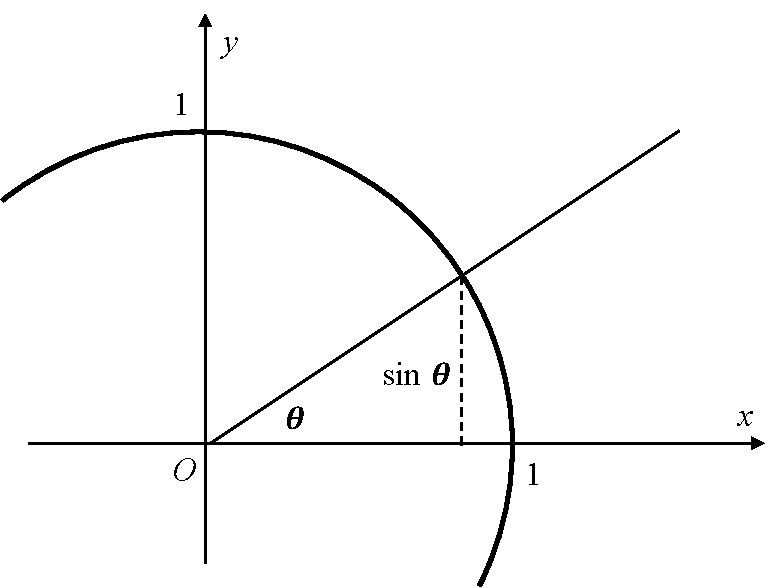
\includegraphics[width=0.6\textwidth]{./Images/ch00/selfTest/triFuncs.pdf}
  \end{figure}
  \item 三角函数的反函数统称为{\kaishu 反三角函数},因为三角函数都是周期函数,
  在整个定义域上不具有统一的单调性,其反函数只能以其某个周期内的一部分为基础来讨论。
  例如:对于正弦函数$y=\sin x$,我们选择其在$[-\pi/2,\pi/2]$上的一段,
  在该区间上$y=\sin x$是严格单调递增的,其反函数记为$y=\arcsin x$
  \ps{相应地反余弦记为$\arccos x$,反正切记为$\arctan x$}。
  $y=\arcsin x$的定义域是$[-1,1]$,值域为$[-\pi/2,\pi/2]$,其图像与
  $y=\sin x$在$[-\pi/2,\pi/2]$区间上的图像关于$y=x$对称。
  从这个例子出发,我们可以很容易地理解讨论反三角函数的基本原则:
  {\kaishu(1)选择三角函数的一个单调区间;(2)所选择的区间
  应该靠近原点,具体来说:要么原点为所选区间的中心,要么为其左端点(也即
  优先考虑正半轴上的区间)}。基于对以上叙述的理解,请分别给出
  $\arccos x$、$\arctan x$的定义域和值域,并试着画出其图像。
  \item 描绘下列函数的图形:
  \begin{center}
    $\sin(\arcsin x),\quad \arcsin(\sin x),\quad
    \tan(\arctan x),\quad \arctan(\tan x)$
  \end{center}
  \item 化简如下表达式
  \begin{enumerate}[(1)]
    \item $\cos(\arcsin x)$
    \item $\sin(\arctan x)$
  \end{enumerate}
  \item 证明:
  $$\df{\pi}4=3\arctan\df14+\arctan\df5{99}$$
  \item 证明:
  $$3\arccos x-\arccos(3x-4x^3)=\pi,\;\left(|x|\leq\df12\right)$$
  \item 平面上任一点的位置可以既可以用直角坐标$(x,y)$表示,也可以用极坐标$(\rho,\theta)$
  表示,前者可用后者表示如下
  $$x(\rho,\theta)=\rho\cos\theta,\quad y(\rho,\theta)=\rho\sin\theta,$$
  反之,后者用前者应表示为(假设:$\rho\geq 0,\theta\in[0,2\pi]$)
  $$\rho(x,y)=\underline{\hspace{5cm}},\quad
  \theta(x,y)=\underline{\hspace{5cm}}.$$
  \item 比较以下函数值的大小,简述理由
  \begin{enumerate}[(1)]
    \item $x,\quad e^x-1,\quad \ln(x+1)$\quad$(x>0)$
    \item $\sin x,\quad \tan x, \quad \sec x, \quad x$ \quad $(x\in(0,\pi))$
  \end{enumerate}
  \item 证明函数$y=x+\sin x$在定义域内严格单调递增。({\it 注:函数$y=f(x)$严格单调
  递增,当且仅当对任意$x_1<x_2$,总有$f(x_1)<f(x_2)$})
  \item 证明:任何一个定义在对称区间上的函数均可写成一个奇函数和一个
  偶函数的和;并由此写出$e^x$是由怎样的奇函数和偶函数相加而成。
  \item 写出下列集合之间的一一映射
  \begin{enumerate}[(1)]
    \item $(-1,1)\mapsto\mathbb{R}$
    \ps{$\mathbb{R}=(-\infty,+\infty)$}
    \item $(0,+\infty)\mapsto\mathbb{R}$
    \item $\{(x,y)\in\mathbb{R}^2|x^2+y^2<1\}\mapsto\mathbb{R}^2$
    \ps{\it $\mathbb{R}^2$表示全平面}
    \item 整数集$\mapsto$正整数集
  \end{enumerate}
  \item Fibnacci数列定义如下:$a_0=1$,$a_1=1$,
  $$a_{n+2}=a_{n+1}+a_{n},\quad n=1,2,\ldots,$$
  \begin{enumerate}[(1)]
    \item 请推导$\{a_n\}$的通项表达式;
    \item 设$p,q\in\mathbb{R}$,将前述递推式改为:
    $$a_{n+2}=p\cdot a_{n+1}+q\cdot a_{n},\quad n=1,2,\ldots,$$
    试讨论$\{a_n\}$通项表达式有何变化。
  \end{enumerate}
  \item 写出不少于五位你听说过的数学家的名字(最好用英文),简述他们的事迹。
  \item 公理(Axiom)、假设(Assumption)、定理(Theorem)、定律(Law)有何异同?
  \item 取整函数$[x]$的定义为{\it 不大于$x$的最大整数},请利用取整函数给出以下曲线的方程:
  \begin{center}
	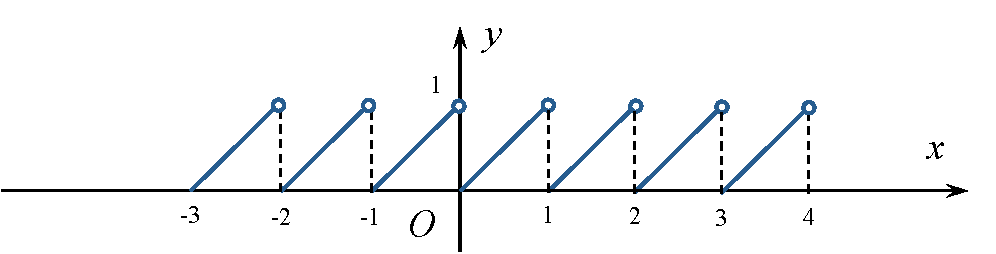
\includegraphics[width=0.8\textwidth]{./images/ch00/selfTest/ST-Func1.pdf}\\
	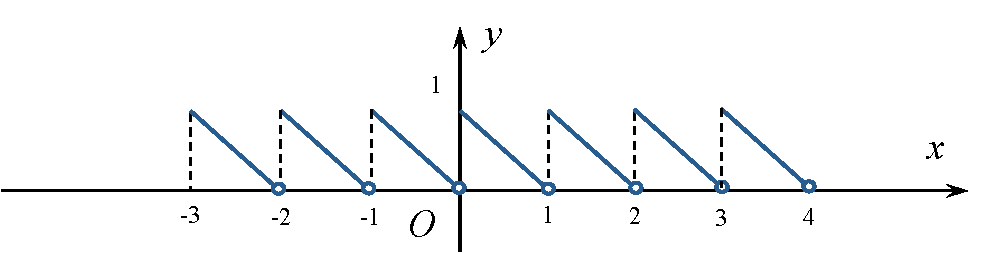
\includegraphics[width=0.8\textwidth]{./images/ch00/selfTest/ST-Func2.pdf}\\
	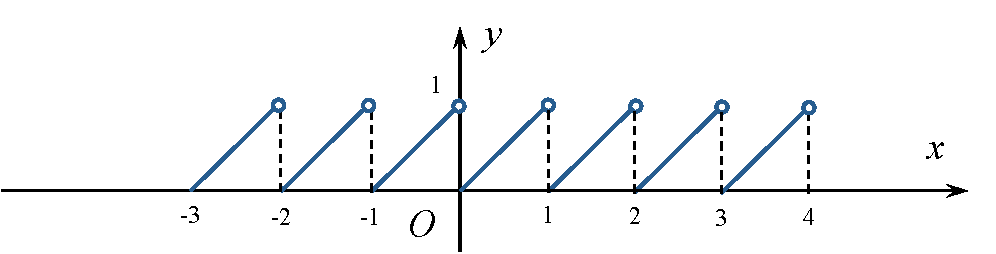
\includegraphics[width=0.8\textwidth]{./images/ch00/selfTest/ST-Func1.pdf}
  \end{center}
  \item 设$a\in\mathbb{R}$,且对任意$x\in\mathbb{R}$,有
  $f(2a-x)=f(x)$,
  请问$y=f(x)$的图像具有怎样的几何性质?若上式改为$f(2a-x)=-f(x)$,对应几何性质有何改变?
  \item 设$a\in\mathbb{R}$,且对任意$x\in\mathbb{R}$,有
  $f(a-x)=g(x)$,请问$y=f(x)$和$y=g(x)$的图像有何关系?
  \item 若对任意$x_1,x_2$,总有
  $[f(x_1)-f(x_2)](x_1-x_2)\leq 0$,
  由此可知函数$y=f(x)$具有何种性质?
  \item 给定集合$A\subset\mathbb{R}$,若$A$有界
  \ps{集合$A$有界,是指存在某个数$M$,对任意$x\in A$,总有$|x|\leq M$},是否必有最大和最小值?
  是否必有{\it 上确界}(即最小的上界)和{\it 下确界}(即最大的下界)?
  若$A$无界,是否必为无穷集合(即集合中的元素个数不是有限的)?
\end{enumerate} % 微积分学前自测

%\section{课程简介}

\subsection{学什么}

高等数学是大学工科专业必修的数学基础课,通常和{\it 线性代数}、{\it 概率论与数理统计}统称
为{\it 工程数学}。

我们所说的高等数学,在国外一般就叫做{\it 微积分},而且通常分为{\it 一元函数微积分}
和{\it 多元(高维)微积分}两个部分。而国外所说的{\it 高等数学}就是我们说的工程数学。

我们一般认为,微积分诞生于17世纪中叶,当时的两位数学巨匠Newton(1642-1726)和
Leibniz(1646-1716)分别独立创立了微积分的理论,并最终被视为微积分的共同发明人。
但是,我们必须认识到的是,一门系统、复杂的理论,不可能仅仅是极个别人的创造。
正如Newton的名言,“{\it If I have seen further, it is by standing on 
the shoulders of giants.}”,在两位大师生前和生后,众多杰出的数学家都为微积分
理论的发展作出了贡献,其中既包括起到奠基作用的Fermat(1607-1665)、Barrow(1630-1677)、
Descartes(1596-1650)%、Huygens(1629-1695)、Wallis(1616-1703)
,也包括使之不断趋于严谨和完善的Cauchy(1789-1857)、D. Bernoulli(1700-1782)、
Lagrange(1736-1913)、Weierstrass(1815-1897)、
Taylor(1685-1731)、Euler(1707-1783)、d'Alembert(1717-1783)
%、Laplace(1749-1827)等
%、Agnesi(1718-1799)
,还有进一步将其发展为更深刻、全面的{\kaishu (数学)分析学}
\ps{分析学和几何学、代数学并称现代数学的三大分支,三者各自拥有庞大的理论体系,
在它们的交汇处诞生了众多重要而又生机勃勃的数学前沿分支}
的
Dirichlet(1805-1859)、Riemann(1826-1866)、Cantor(1845-1918)、
Lebesgue(1875-1941)、
Fourier(1772-1837)等。今天我们所学习的微积分,虽然只是分析学
的基础部分,但要说其中融汇了300多年来众多近现代数学家的杰出成就,是绝对实至名归的。

% \begin{figure}[htbp]
% 	\centering\scalebox{0.3}{\includegraphics{./images/ch1/AM_architecture.jpg}}
% 	\caption{微积分中的主要概念及其关系\;
% 	({\it 个人整理,仅供参考})}
% % 	\label{图:0.1}
% \end{figure}

% \begin{center}
% 	\scalebox{0.3}{\includegraphics{./images/ch1/AM_architecture.jpg}}
% % 	\ps{上课前画好}
% \end{center}

%\begin{center}
%	\includegraphics[width=0.8\textwidth]{./images/ch1/AM_architecture.jpg}
%	
%	{微积分中的主要概念及其关系\;
%	({\it 个人整理,仅供参考})}
%\end{center}

%\begin{center}
%	\includegraphics[width=0.8\textwidth]{./images/%ch1/AM_architecture.jpg}
	%\caption{微积分中的主要概念及其关系}
%\end{center}

\begin{figure}[htbp]
	\centering
	\includegraphics[width=0.8\textwidth]{./images/ch00/AM_architecture.jpg}
	\caption{微积分中的主要概念及其关系\\ ({\it 个人整理,仅供参考})}
\end{figure}

\begin{itemize}
	  \item {\bf 微积分(Calculus)} \hfill from Wikipedia
	\begin{itemize}
	  \item Latin: {\it a small stone used for counting}  
	  \item {\it a branch of mathematics focused on \underline{limits, functions,
	  	derivatives, integrals, and infinite series}} 
  	  \item {\it widespread application in \underline{science, economics,} 
  	  and \underline{engineering}} 
	  \item {\it constitues a major part of modern mathematics}
	  \item {\it 微}的意思是很小的东西,如微生物,{\it 积}就是加起来的意思,
	  {\it 积分}的意思就是把极小的东西加起来。微,是积的相反。 
	\end{itemize}
	\item {\bf John von Neumann} ({\small\it The Mathematician, 1947})
	\begin{itemize}
	  \item {\it The calculus was the \underline{first achievement} of modern
	  mathematics, and it is difficult to overestimate its importance.}
	\end{itemize} 
\end{itemize}

\subsection{为什么学}

微积分为什么如此重要,毫无疑问,与其在众多领域的应用密不可分,甚至可以说,
在其中绝大多数的问题中,微积分的作用是无可替代的。任何一门工科类的专业课程,
只要涉及与连续运动(变化)相关的问题,都不可避免地会以微积分作为其预备知识,
或者说,将这些课程视为微积分的应用也不为过。

当然,微积分不总是“美丽”的,因为它的美可能不是那么显而易见。我们很难用一两句话
来描述,微积分到底有什么用?它美在哪里?但是,一旦你理解了微积分背后的深刻思想,
开始能够将其应用于解决一些实际问题,或者通过它理解一些最前沿的科技成就时,
你一定会对它的美产生深深地赞叹,也许那时,再回头来看微积分的重要性也就不言而喻了。

学习微积分的过程也许会有些枯燥甚至痛苦\ps{“从前有棵树,叫高数,上面挂了很多人”}
,但它无疑是值得的,能够从看似单调痛苦的过程中领略数学的美丽,发现它的深刻与强大,
也是它作为“{\it 大学第一课}”\ps{无论从体量、难度还是学习的先后来看}所期望带给
大家的体验。

\begin{shaded}
	{\bf 知乎:学数学有什么好处?我们为什么要学数学?}
	\begin{itemize}
	  \item Engles:{\it 数学是一门研究现实世界的数量关系和空间形式的科学。}数学具有:
	  抽象性、精确性和应用的广泛性
	  \item Marx:{\it 一种科学只有在成功运用数学时,才算达到了真正完善的地步。}
	  \item Galileo:{\it “数学符号就是上帝用来书写自然这一伟大著作的统一语言,
	  不了解这些文字就不可能懂得自然的统一语言,只有用数学概念和公式所表达的物理世界
	  的性质才可认识……”}
	  \item Gauss:{数学是科学的女王}
	  \item 韩寒:{\it
	  我们生活中用到的数学估计到小学三年级就已经够用了。}然而在之后我们多年来学习的数学,
	  实际上塑造了我们一种理性的、条理的、系统化的思维方式。这种思维方式在我们解决自己
	  一生中遇到的诸多问题时,都有非常重要的作用。比如慎密的思考、分类的思想、排序的思想等。
	  很多东西其实都带有学习数学这个过程产生的影响,只是由于其作用方式非常隐晦,
	  也不容易被追溯其源头,我们平时不容易注意到罢了。
	  \item 王小波:{\it 我上大学时,有一次我的数学教授在课堂上讲到:我现在所教的数学,
	  你们也许一声都用不到,但我还要教,因为这些知识是好的,应该让你们知道。”}
	  \begin{enumerate}
	  	\item 用通用简洁的方式来表达自然规律
	  	\item 提供一些问题的分析手段
	  	\item 提供认识世界的一种模式
	  	\item 了解自己的智力水平
	  \end{enumerate}
	\end{itemize}
\end{shaded}

\begin{itemize}
  \item {\bf 数学的三大功能}
  \begin{enumerate}
    \item 为学习其他知识(课程)提供数学工具
    \item 培养理性思维
    \item 弘扬数学文化
  \end{enumerate}
  \item {\bf 数学素质}
  \begin{enumerate}
    \item 从实际问题抽象出数学模型的能力
    \item 计算与分析的能力
    \item 了解和使用现代数学语言和符号的能力
    \item 使用数学软件学习和应用数学的能力
  \end{enumerate}
\end{itemize}

\subsection{怎么学}

\begin{itemize}
	\item {\bf 参考资料}
  	\begin{enumerate}
		\item {\bf 课程配套辅导}
	  	\begin{itemize}
	  	  \item \underline{同济大学数学系,高等数学(第七版,上、下),高等教育出版社,2014,北京}
	  	  	\ps{简称:\b 同济}  
	  	  \item 朱健民 等,高等数学(第二版,上、下),高等教育出版社,2015,北京
	  	  	\ps{简称:\b KD教材} 
	      \item 李建平 等,高等数学典型例题与解法(上、下),国防科技大学出版社,2009,长沙
	    	\ps{简称:\b 辅导书} 
	  	\end{itemize}
  		\item {\bf 参考书} 
  		\begin{itemize}
	    	\item 菲赫金哥尔茨,微积分学教程(第一至三卷),第8版,高等教育出版社,2006,北京
	    	  \dotfill{\it\b 读不懂不必勉强,它回答不了的微积分问题大学阶段你肯定碰不到} 
	    	\item James Stewart, Calculus(11th eds.)(影印版,上、下册),高等教育出版社,2016,北京
	    	  \dotfill{\it\b 大部头,但绝对浅显易懂}
	    	\item 斯蒂芬.弗莱彻.休森,数学桥,上海科技出版社,2010,上海
	    	  \ldots\dotfill{\it\b 值得常常拿出来读的数学书,一遍绝对不够} 
	    	\item William Dunham,微积分的历程——从牛顿到勒贝格,人民邮电出版社,2011,北京
	    	\dotfill{\it\b 了解微积分的历史,能够更好地理解其中深刻的思想} 
  		\end{itemize}
  		\item {\bf 在线资源}
  		\begin{itemize}
  		  \item 朱健民,高等数学(一-五),中国大学MOOC%,http://www.icourse163.org/course/NUDT-9004
  		    \ps{简称:\b MOOC}\ldots
  		    \dotfill{\it\b 缺课或者课上没听懂,就用它补补课}
  		  \item 李建平\,等,高等数学典型例题与解法(一、二),中国大学MOOC%,\\
  		    %http://www.icourse163.org/course/NUDT-1001979006
  		    \ldots\dotfill{\kaishu\b 辅导书的配套MOOC}
  		  \item 闫浩,高等数学习题课,学堂在线%,\\
  		     %https://xuetangx.com/courses/course-v1:BUPT+3412113011+2017_T2/about
  		     \dotfill{\it\b 讲得棒极了,这老师其实是清华的}
%   		  \item 李建平\,等,微积分CAP,中国大学MOOC%,
  		     %http://www.icourse163.org/course/NUDT-1001626005
%   		    \dotfill{\it\b 高中没学好,来这补一补}
		\end{itemize} 
		\item {\bf 扩展阅读}\dotfill{\it\b 读一些课外书,让学习显得不那么枯燥}
		\begin{itemize}
		  \item 基斯.德夫林,数学思维导论,人民邮电出版社,2016,北京
		  \item G.波利亚,怎样解题:数学思维的新方法,上海科技教育出版社,2011,上海
		  \item 李学数,数学与数学家的故事(1-5),上海科学技术出版社,2015,上海
		  \item 塞德里克·维拉尼\,等,一个定理的诞生:我与菲尔茨奖的一千个日夜,人民邮电出版社,2016,北京
		  \item 春日真人,庞家莱猜想:追寻宇宙的形状,人民邮电出版社,2015,北京
		  \item 蒂莫西.高尔斯,数学,译林出版社,2014,南京
		  \item 吴军,数学之美,人民邮电出版社,2016,北京
		  \item 李建平,漫谈数学与军事,中国大学MOOC
		  \item \ldots\ldots
		\end{itemize}
	\end{enumerate}
	\item {\bf 学习方法}
% 	\begin{itemize}
% 	  		\item {\bf 听课}\dotfill {\bf 30}
% 		\begin{itemize}
% 	  		  \item 典型问题、典型方法
% 	    	  \item 师傅领进门,修行在个人
% 	 	\end{itemize}
% 	  		\item {\bf 练习}\dotfill {\bf 50}
% 	 	\begin{itemize}
% 	    		\item 熟能生巧!
% 	    		\item 记忆!琢磨!
% 	  	\end{itemize}
% 	  		\item {\bf 思考}\dotfill {\bf 20}
% 	  	\begin{itemize}
% 	    		\item 总结!
% 	    		\item 质疑!
% 	  	\end{itemize}
% 	\end{itemize}
	\begin{enumerate}
	  \item {\bf 预习:}课前3-5分钟,快速翻阅教材,浏览本讲内容梗概,
	  标记出新的名词和例题,试着理解其大概意思,确保听课时心中有数;
	  \item {\bf 听课:}抓住关键思路,卡住了或者有疑点立即举手问,
	  简要记笔记\ps{推荐:\b 康奈尔笔记法},重点记思路和书本上没有的内容
	  \item {\bf 复习:}要么读教材,要么读笔记,也可以先作习题,搞不定
	  再回来翻书查笔记,重在理清思路\ps{重要概念,典型问题,典型方法},
	  消化细节,肯花时间才有好的效果
	  \item {\bf 练习:}作业之外,有选择地作题,学习也是个熟能生巧的过程,
	  提高效率是关键\\
	  G.Polya:{\it 我们的任何一门学问都由知识和技能组成。如果你对初等或高等数学的研究工作
	  的确有真正的经验的话,那么你对下述这一点将毫不怀疑:在数学中,技能比仅仅掌握
	  一些知识要重要得多。什么是技能呢?数学技能就是解题能力——不仅能解决一般的问题,
	  而且能解决需要某种程度的独立思考、判断力、独创性和想象力的问题}
	  \item {\bf 思考:}多琢磨,让知识点在大脑中结成网络,融会贯通,
	  会提问是思考能力的体现\ps{Einstein:提出一个问题往往比解决一个问题更重要!}
	  \centerline{\it What$\to$How$\to$Why$\to$Why not$\to$What if}
	\end{enumerate}
\end{itemize}

\section{几点要求}
\begin{itemize}
	\item {\bf 课堂:安静!安静!!安静!!!}
	尊重他人学习的权利,安排好自己的时间
	
	{\bf - No to}
	  \begin{itemize}
	    \item Chatting
	    \item zZZ\ldots
	    \item anything noisy
	    \item \ldots
	  \end{itemize}
	{\bf - Yes to}
  \begin{itemize}
    \item listen to me
    \item discuss {\bf with me}
    \item do sth. you like {\bf quietly}
    \item zzz\ldots
    \item leave/enter the classroom {\bf quietly}
    \item \ldots
  \end{itemize}
  \item {\bf 作业}
  \begin{figure}[h]
  	\begin{center}
  		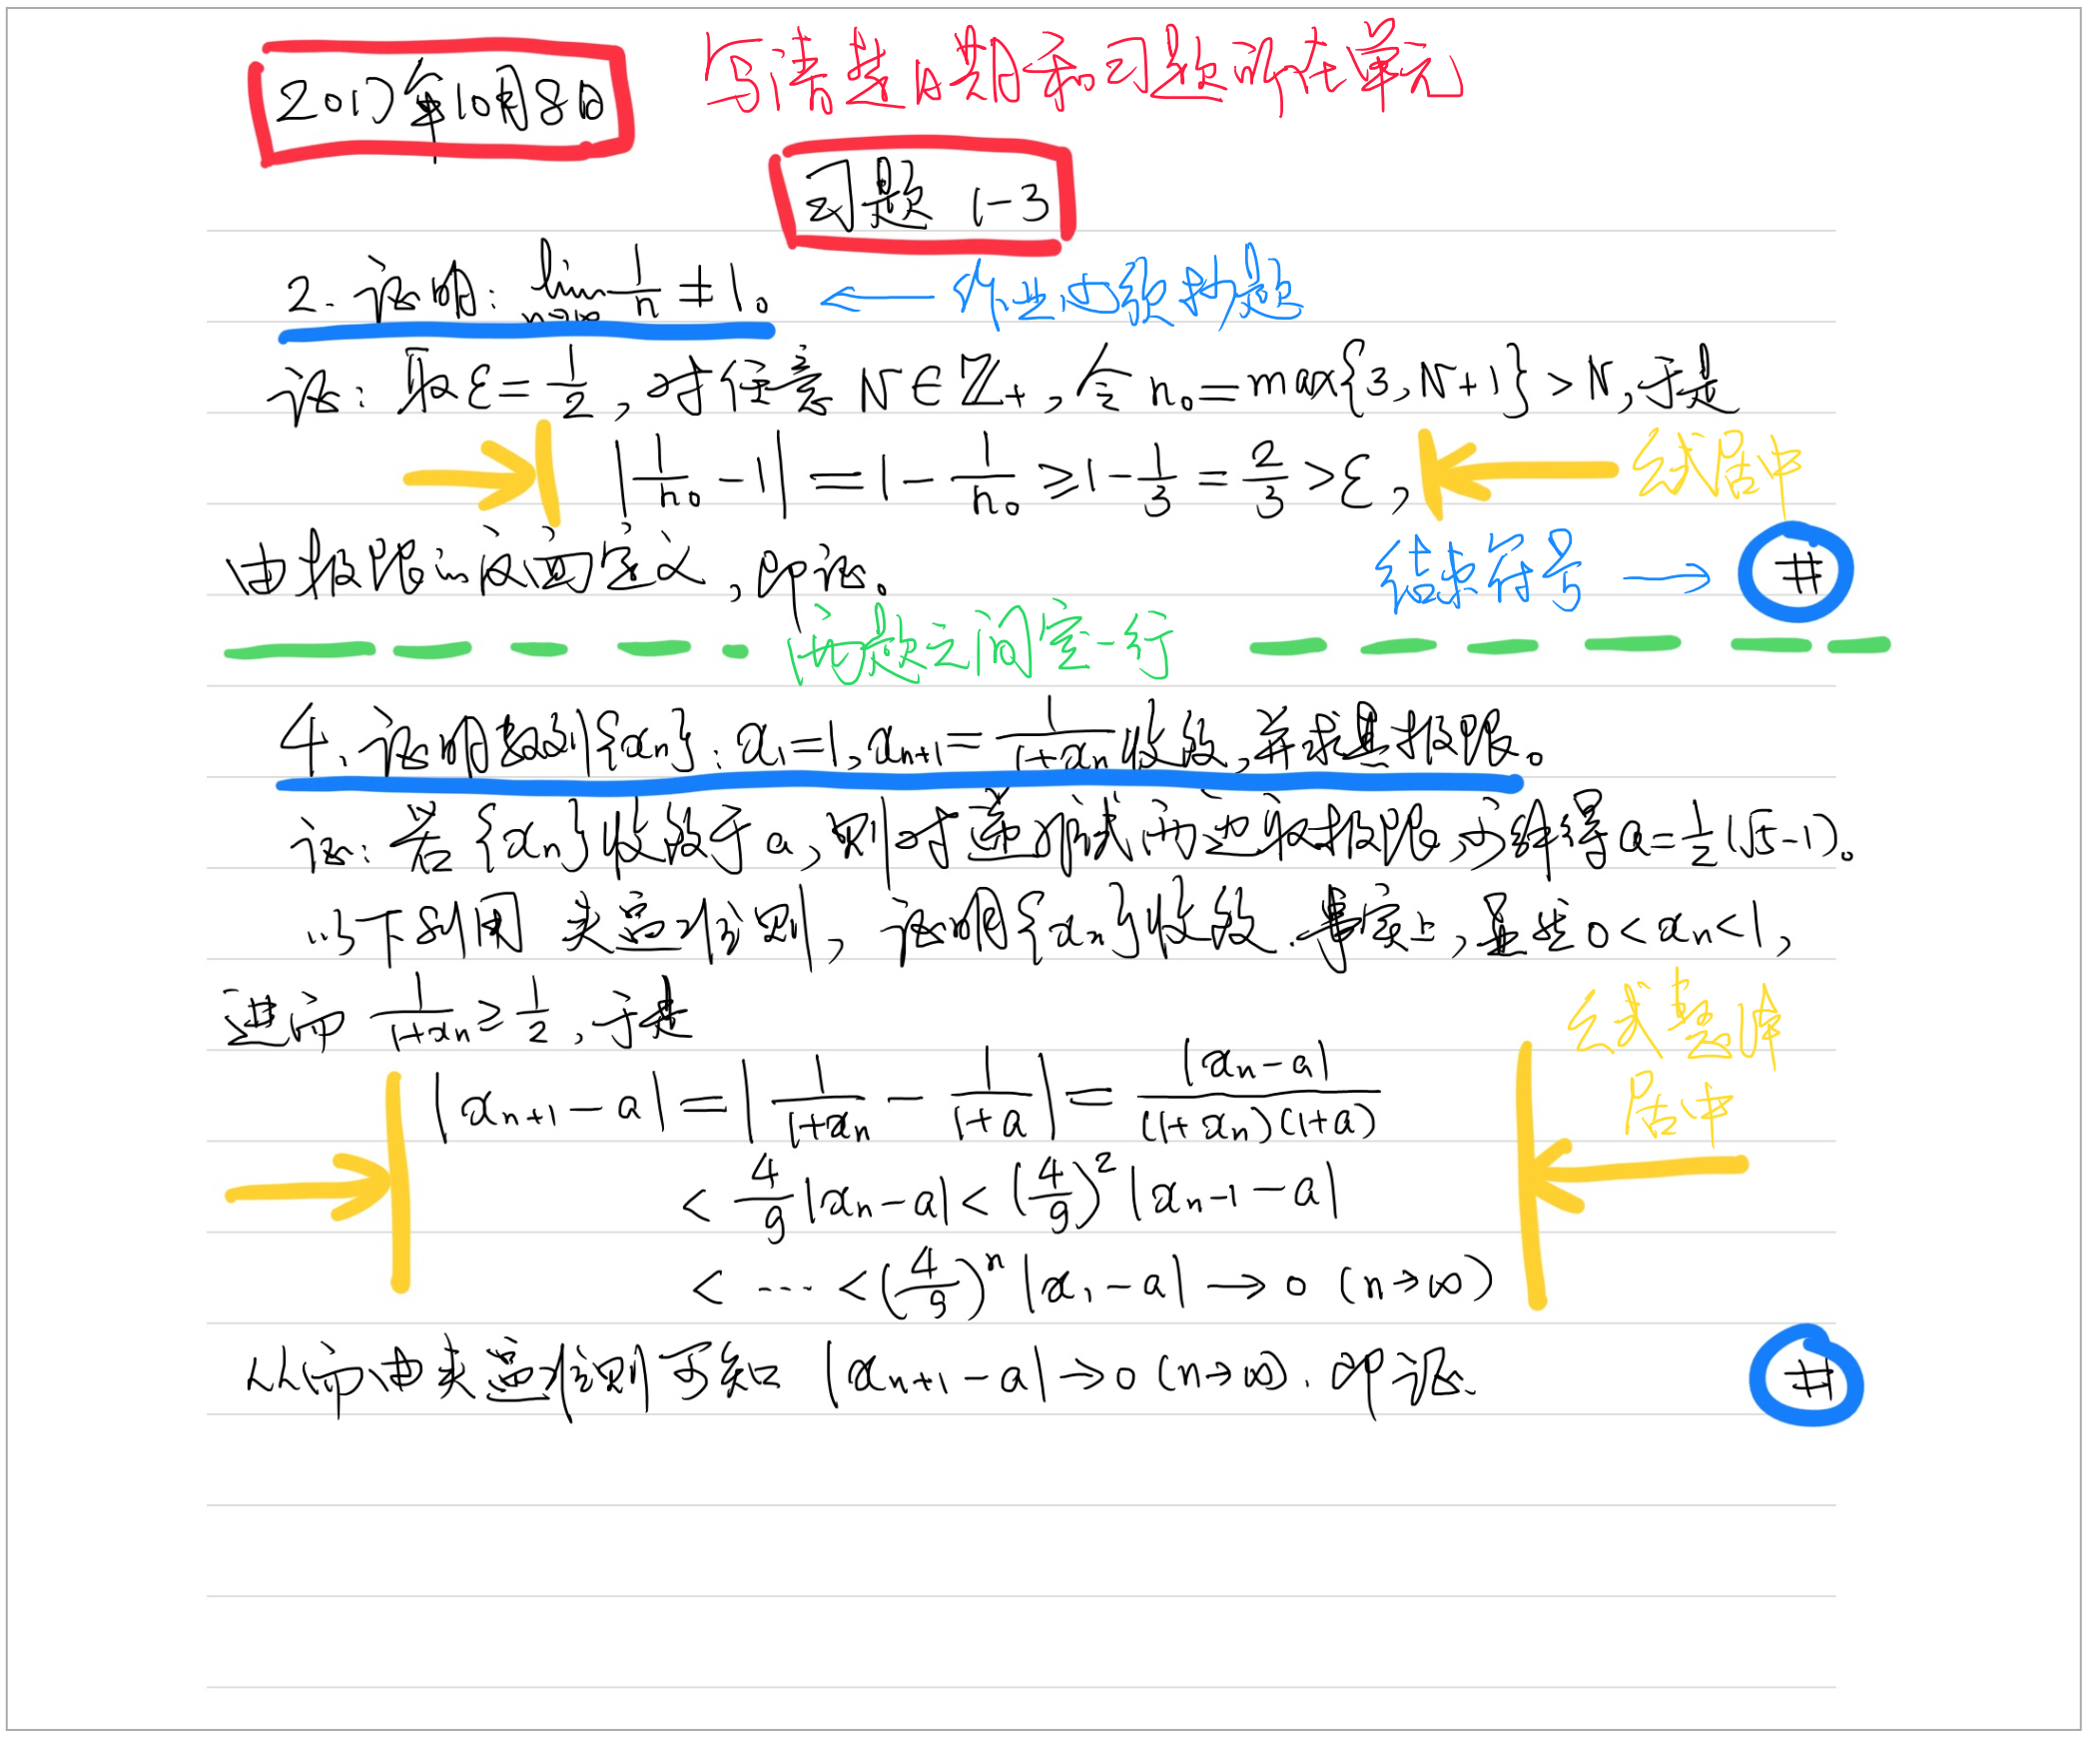
\includegraphics[width=0.95\textwidth]{./images/Ch00/hw-sample.jpg}
  		\caption{作业参考格式\\ (以黑色字体为准,彩色部分为格式说明)}
  		\label{fig:0.2}
  	\end{center}
  \end{figure}
  \begin{itemize}
    \item 基本规范
    \begin{enumerate}
      \item 写清楚作业日期(对应讲课的日期)和习题所在单元;
      \item 作业必须抄题,写清楚题号
	  \item 解题过程以“证:”或“解:”开始,以$\#$号结束;
	  \item 公式整体居中书写;
	  \item 无论大题小题,两题之间空一行;
	  \item 不允许使用铅笔、红笔书写作业,可以用铅笔画图;
	  \item 作业本不许分栏使用;
	  \item 文字、符号书写清晰规范,尽量少涂改。
    \end{enumerate}    
    \item no copy ??!
    \item 及时订正错误,补上缺漏
  \end{itemize}
	\item {\bf 答疑}
	  \begin{itemize}
	    \item 每周一次面对面答疑,1-2小时
	    \item 提问题的能力不完全是天生的,脸皮要厚一点
	    \item 综合利用各种手段(微信、网站、邮件、\ldots)
	  \end{itemize}
% 	  \item {\bf 从善如流}
\end{itemize}

\section{关于考试}

以下是2017-2018学年开始实施的“{\it 新政}”:

考试分为{\it 形成性考试}和{\it 终结性考试}两个部分,两部分成绩按照$40\%$和$60\%$的比例综合
得到最终的课程期末成绩。

每学期末设一次终结性考试,采用闭卷笔试形式。{\color{red}\bf 终结性考试不及格,
则课程成绩不合格!}

每学期的形成性考试分为四个部分,一是{\it 平时作业和表现}成绩,占$10\%$,剩下的为三次
{\it 单元测试}成绩,各占$10\%$。

单元测验的形式为笔试或网络测试,具体待定。

\begin{ext}
	\begin{center}
		\bf 课后作业
	\end{center}
	
	%{\b\it 说明:作业必须写明题目所在章节、页码、题号;如非特别说明,
	%所有题目必须抄题;两道题之间空一行;未作或作错的题目讲评后务必及时订正。}
	
	\begin{enumerate}
	  \item 加老师的QQ:20847517,发送自己的姓名作为验证信息;
	  \item 注册中国大学MOOC账号:http://www.icourses.cn/imooc/,将“学号、姓名、账号”告知课代表统一登记,同时选择加入我校自己开设的
	  《高等数学(一)》、《高等数学典型例题与解法(一)》及
	  《漫谈数学与军事》三门课程;
	  \item 写一篇短文,内容及要求如下:
	  \begin{enumerate}[(1)]
	    \item 你的个人介绍,请务必包含如下信息:姓名、性别、年龄、籍贯、
	    中学母校的名字、你的高考总成绩(以及当地的满分)、
	    你的高考数学成绩(以及当地的满分);
	    \item 你的兴趣爱好、特长,或者说,你觉得自己有什么与众不同之处;
	    \item 你学习数学的体会,例如:喜欢什么样的数学,不喜欢什么样的数学?
	    有什么你个人觉得比较好的学习方法、成功的经验,或者有趣的经历
	    (最好与数学有关)?
	    \item 你对大学的课堂有什么期待?怎么样的教与学会对你更有帮助?
	    对老师有什么要求或者建议?
	    \item 请至少推荐一本(部、套)你喜欢的书、电影或者其他任何可以
	    通过公共渠道获取到的资料(例如:网站、软件、APP、\ldots),说说推荐的理由;
	    \item 其他任何你认为值得(可以)与老师交流的东西,比如你想问我什么
	    都可以问;
	    \item 除第一条必须包含外,其余内容可自由取舍;
	    \item 篇幅不少于半页活页纸(A4或16K),不多于两页(一张的正反面)。
	  \end{enumerate}
	  \item 自行了解学习康奈尔笔记法(本章附录);
	  \item 自行阅读李开复博士的《给未来的你》(稍后会发在课程的QQ群内)。
	\end{enumerate}
\end{ext}

\newpage

{\bf 附录:Cornell Note-Taking System}\hfill{\it 康奈尔笔记法(5R笔记法)}

这一方法适用于一切依赖讲授或自学的学习过程,特别是对于听课笔记,5R笔记法堪称首选。
该方法的重点是记与学、思考与运用的结合,以及将笔记的记录与完善作为学习的过程载体。
最终完成的笔记类似于下图:

\begin{figure}[h]
	\centering
	\begin{subfigure}[t]{0.45\textwidth}
		\centering
		%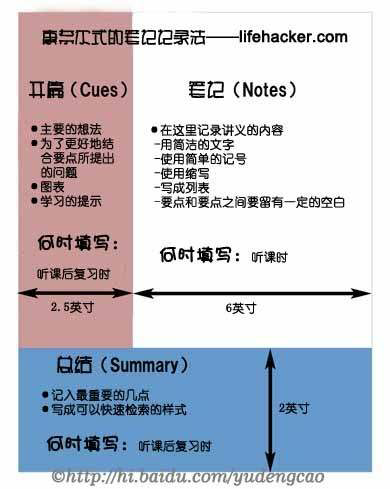
\includegraphics[height=8cm]{./images/Ch00/Cornell-NTS/NTS-CH.jpg}
		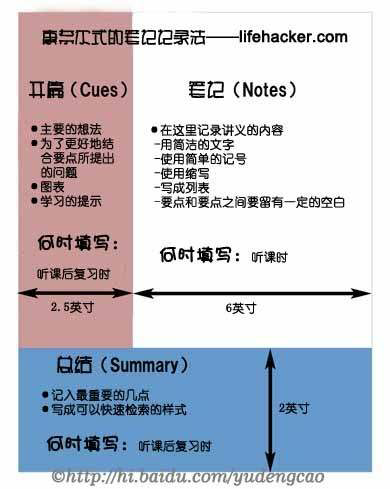
\includegraphics[width=\textwidth]{./images/Ch00/Cornell-NTS/NTS-CH.jpg}
		\caption{布局}\label{fig:5R-1}
	\end{subfigure}
	\begin{subfigure}[t]{0.45\textwidth}
		\centering
		%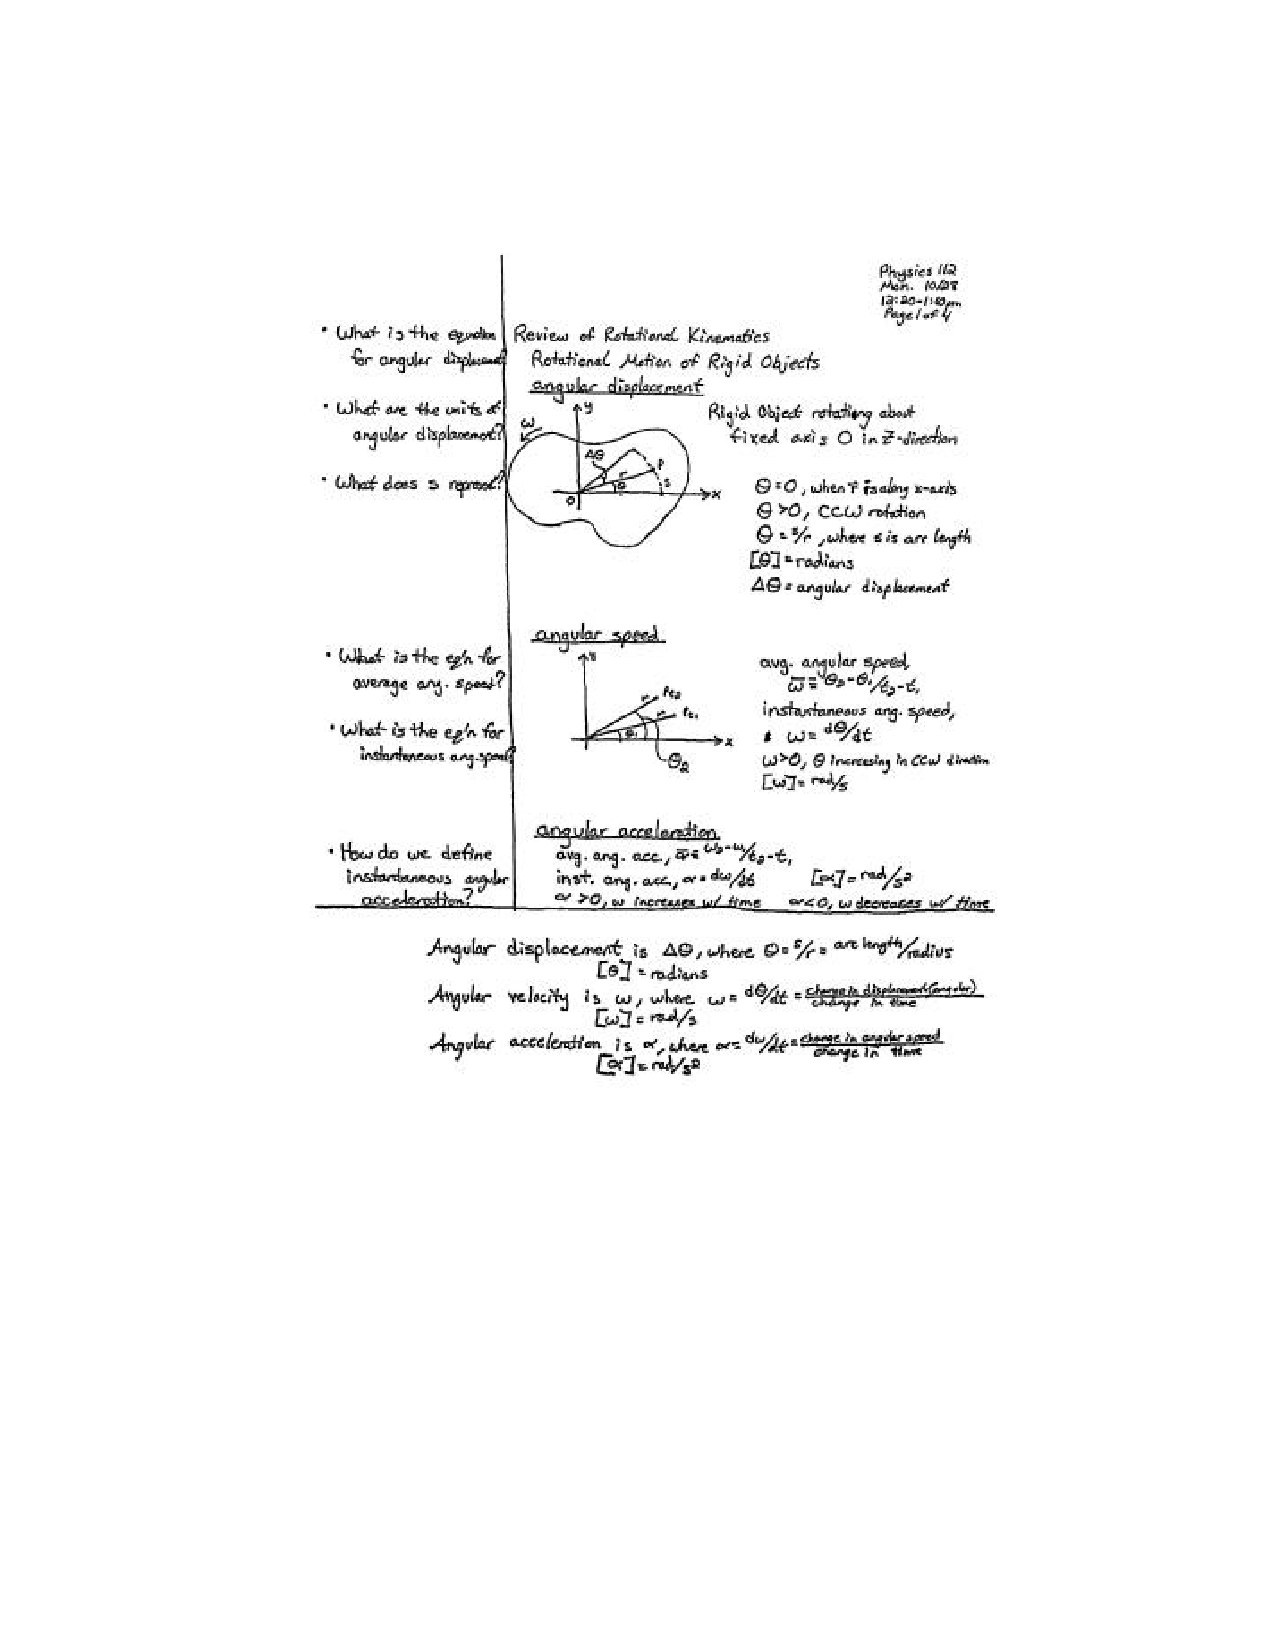
\includegraphics[height=8cm]{./images/Ch00/Cornell-NTS/exCNTS.pdf}
		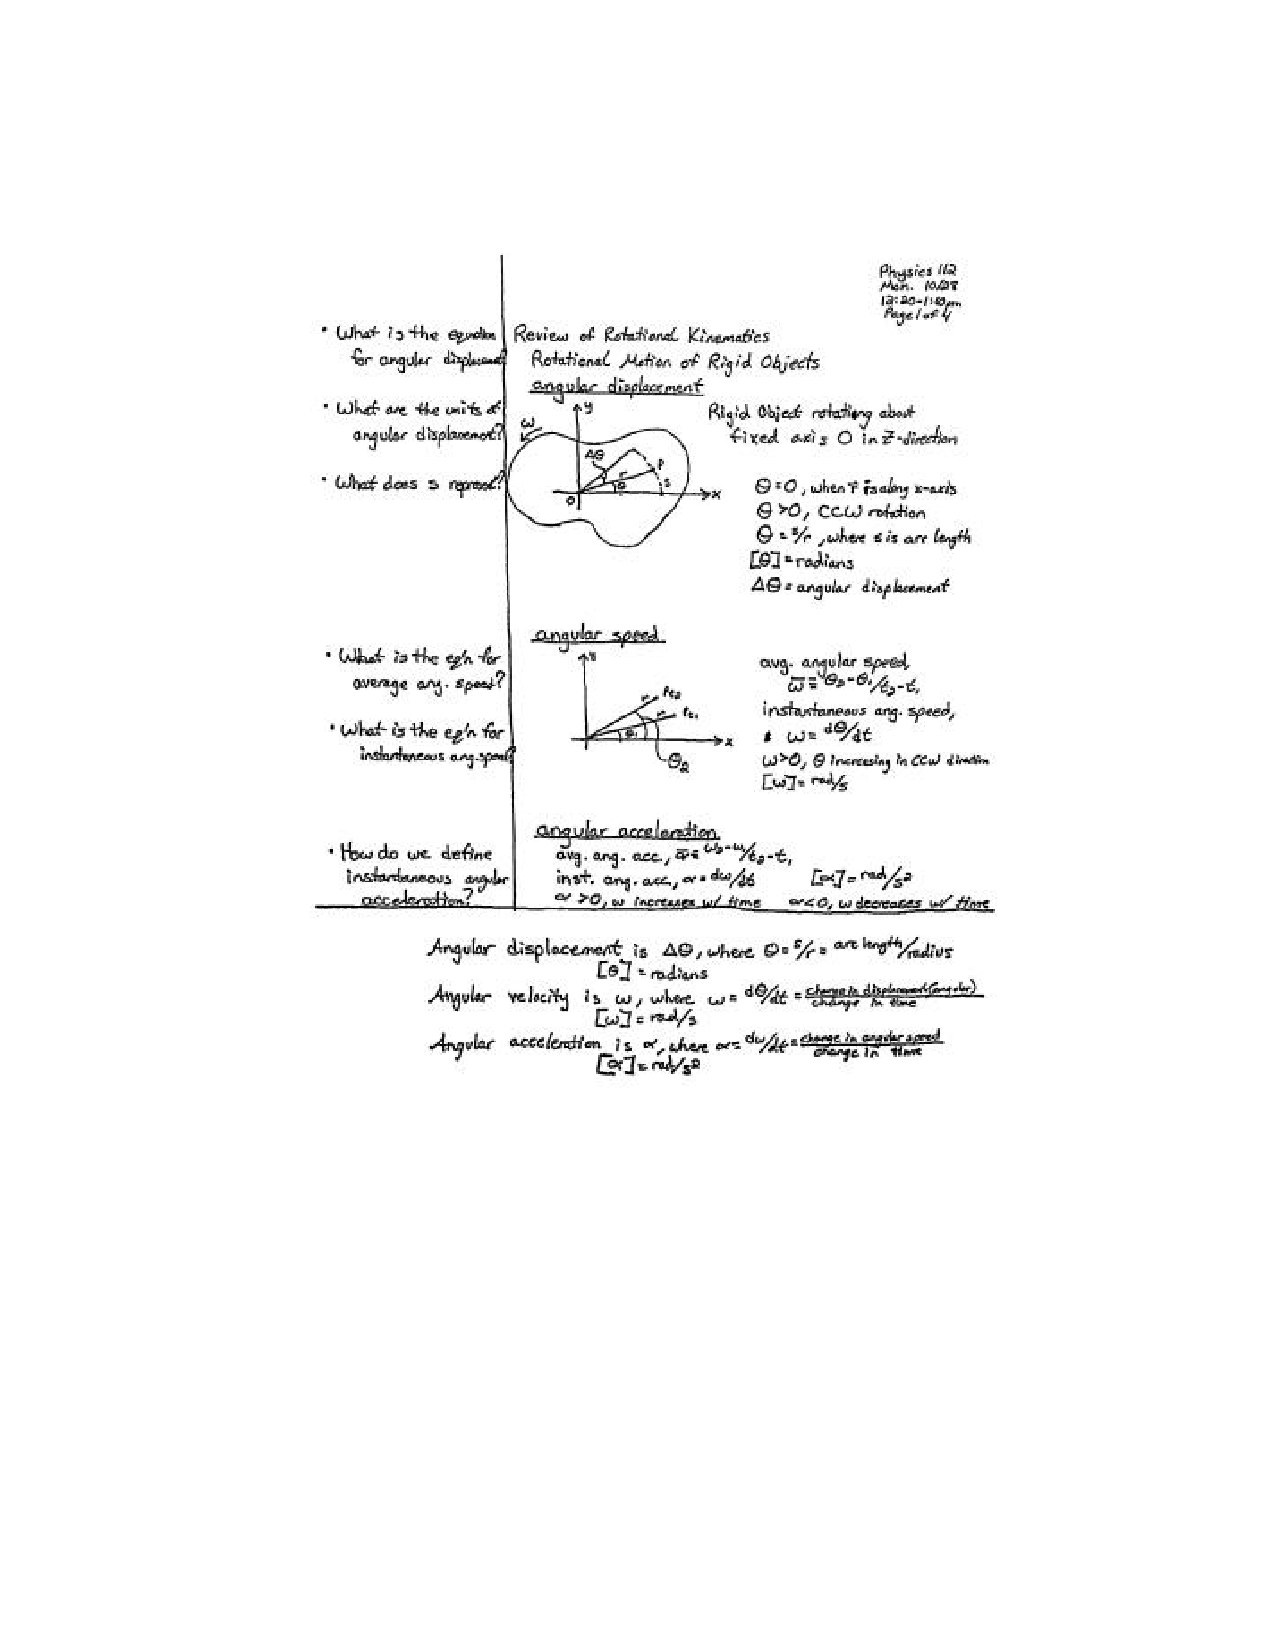
\includegraphics[width=\textwidth]{./images/Ch00/Cornell-NTS/exCNTS.pdf}
		\caption{示例}\label{fig:5R-2}
	\end{subfigure}
	\caption{5R笔记法}\label{fig:5R}
\end{figure}
	
笔记的行程过程可以分为所谓的{\bf 5R}:

\begin{enumerate}[Step1]
  \setlength{\itemindent}{1cm}
  \setlength{\topsep}{0pt}
  \item {\it 记录(Record):}在听讲或阅读过程中,
  在主栏(将笔记本的一页分为左大右小两部分,
  左侧为主栏,右侧为副栏)内尽量多记有意义的论据、概念等讲课内容。
  \item {\it 简化(Reduce):}下课以后,尽可能及早将这些论据、概念简明扼要地概括(简化)
  在回忆栏,即副栏。
  \item {\it 背诵(Recite):}把主栏遮住,只用回忆栏中的摘记提示,
  尽量完满地叙述课堂上讲过的内容。
  \item {\it 思考(Reflect):}将自己的听课随感、意见、经验体会之类的内容,
  与讲课内容区分开,写在卡片或笔记本的某一单独部分,加上标题和索引,
  编制成提纲、摘要,分成类目。并随时归档。
  \item {\it 复习(Review):}每周花十分钟左右时间,快速复习笔记,主要是先看回忆栏,
  适当看主栏。
\end{enumerate}

在课本、参考书原文的旁边加上各种符号(如直线、双线、黑点、圆圈、
曲线、箭头、红线、蓝线、三角、方框、着重号、惊叹号、问号等等),便于找出重点,
加深印象,或提出质疑。什么符号代表什么意思,自己掌握即可,但最好形成一套比较
稳定的符号系统。这种方法特别适合于自学笔记和预习笔记。

操作时注意以下一些准则:
{\it 读完后再做记号,要非常善于选择,用自己的话进行注记,形式和过程力求简洁,迅速,整齐}

笔记的加工:{\it 忆$\to$补$\to$改$\to$编$\to$分$\to$舍$\to$记}	
 	% 课程简介与学习要求

% !TEX root = ../0-main-LN.tex

\setcounter{theExample}{1}

\chapter{函数与极限}

函数与极限是微积分理论中最基础和最核心的概念,也是定义
微分和积分的基础。熟练掌握常用函数的特性,理解极限的概念与性质,
并会在一定程度上加以应用,是真正理解微积分的第一步。

极限的定义(更具体地称为“$\e-\delta$”或“$\e-N$”定义)可能是大多数人
在微积分学习中遇到的第一个难点(因人而异),因为它兼具形式的抽象性和
逻辑的复杂性(必须严谨、准确)。学会用数学和逻辑的语言表达某个概念、某个
命题,并能将推理、分析的过程严谨、准确地叙述出来,也是通过微积分的学习
需要锻炼和培养的能力。

\section{集合、映射与函数}

\subsection{集合}

我们目前使用的集合概念,一般被认为来源于数学家Cantor的定义(1974),
他的表述是:所谓{\it 集合},是指把一些个体({\it 元素}) 
放在一起考虑时所形成的整体。
\ps{对于集合,“我们只需描述它,而不必给出精确的定义”}

我们可能用到的相关的符号可分为两类:
\begin{itemize}
  \item 关系符号:$\subset, \in, =, \subseteq, \neq$
  \item 运算符号:$\cap,\cup, \setminus, \bar{A}, \times, +, - $\quad ({\it
  依次为:交、并、差、补、笛卡尔积、不交并、差})
\end{itemize}
	
本门课程中常见(用)的集合有:
$$\mathbb{N}\subset\mathbb{Z}\subset\mathbb{Q}
\subset\mathbb{R}\subset\mathbb{C}$$
从左到右依次为:{\kaishu 自然数集}
\ps{\vspace{-1cm}国内教材一般约定,自然数集包含数$0$}、
{\kaishu 整数集}\ps{Z是德语Zahlen(数)的首字母}、{\kaishu 有理数集}
、{\kaishu 无理数集}和{\kaishu 复数集}。

通过集合的{\it 笛卡尔积}“$\times$” 可以定义更{\it“高维”}的集合,
例如:$\mathbb{R}$表示数轴(上的所有点构成的集合),则
$$\mathbb{R}^2=\mathbb{R}\times\mathbb{R}$$
表示全平面(上的所有点构成的集合)。

\subsubsection*{区间和邻域}

讨论函数的定义域和值域是,我们常常会用到区间和领域这两个概念。

具体来说,给定$a,b\in\mathbb{R},a<b$,可定义一个开区间
$$(a,b)=\{x\in\mathbb{R}|a<x<b\}.$$

一般来说,我们记实数集
$$\mathbb{R}=(-\infty,+\infty)$$

{\baa 注意:由于$\pm\infty$都不是具体的数,因此在本门课程中,
除非特别说明,形如
$$x=+\infty\quad\mbox{或}\quad x=-\infty$$
的写法总是错误的,而只能写
$$x\to+\infty\quad\mbox{或}\quad x\to\infty.$$
}

{\bf 邻域}是区间的另一中表示方法,它的一般形式为
$$U(x_0,\delta),$$
其中$x_0$表示邻域的中心,$\delta$为领域的半径,如非特别说明,
领域一般为开区间。例如:
$$U(a,\delta)=(a-\delta,a+\delta)=\{x\in\mathbb{R}||x-a|<\delta\}.$$
$U(x_0,\delta)$的直接解释是:实数中所有与$x_0$的距离(差的绝对值)
小于$\delta$的数(点)构成的集合。

\bs

{\bf 课堂练习:}$(a,b)=\underline{\hspace{4cm}}$
\ifhint\ps{$U\left(\df{a+b}2,\df{b-a}2\right)$}\fi

\bs

有时候,我需要考虑不包含中心的领域,也即{\kaishu 去心领域},记为
$$
U_0(a,\delta)\quad\mbox{或}\quad U^0(a,\delta)$$
对应的区间为$(a-\delta,a+\delta)-\{a\}$
(或$\{x\in\mathbb{R}|0<|x-a|<\delta\}$)。

有时候,我们也会用到所谓的{\kaishu 无穷邻域},其定义为
$$\{x\in\mathbb{R}||x-x_0|>M\},\;M>0,$$
表示与点$x_0$的距离超过$M$的所有点构成的集合。我们可以将无穷领域想象
成以{\kaishu 无穷远点}\ps{\baa因为无穷远点不是一个数,为了避免误解,我们不会将无穷邻域写成
类似$U(\infty,M)$的形式}
(现实中是不存在的)为中心的领域。

最后,还有所谓的{\kaishu 左(右)半邻域},例如:点$a$的右半邻域为
$$\{x\in\mathbb{R}|a<x<a+\delta\}.$$

\bs
\centerline{注:灰色底色部分的内容为扩展知识,了解即可,不要求掌握}
\begin{shaded}
	{\bf 集合论、Russell Paradox与公理系统}

	Cantor在1874年提出的集合概念及其相关的理论——统称{\kaishu 集合论},通常被也称为{\kaishu 朴素集合论}。集合论的提出为整个数学的研究
	奠定了重要基础,使得众多的数学理论得以变得更加严谨和系统。对于这一
	成就,历史上有过一些重要的评述,其中被广泛传播的是Poincaré在1900的
	国际数学家大会所说:{\kaishu
	 “\ldots 借助集合论概念,
	 我们可以建造整个数学大厦\ldots  
	 今天,我们可以说绝对的严格性已经达到了\ldots”}。
	
	然而,现实其实并不那么乐观,1901年,英国数学家——也有人说是哲学家
	——Russell提出了他著名的悖论

	\pss{\centering
	\includegraphics[width=0.7\marginparwidth]{./images/ch01/Russell.jpg}\\
	\href{https://en.wikipedia.org/wiki/Bertrand_Russell}{B. Russell(1872-1970)}
	}

	\centerline{\kaishu 只给不给自己理发的人理发的理发师该不该给自己理发?}
	
	转换成集合论的语言,可以表述为:

	\centerline{\kaishu 由所有不包含集合自身的集合所构成
	的集合是不是一个集合?}

	其中的矛盾是非常明显的。设$A$为上述集合,则
	$$A=\{x|x\notin x\}.$$ 
	如果$A\in A$,则根据以上定义,$A\notin A$;反之,如果$A\notin A$,
	则必有$A\in A$。

	那么到底是$A\in A$还是$A\notin A$呢? 一个简单的命题居然导出了
	自相矛盾的结论,这从根本上动摇了数学大厦的根基。Cantor的集合定义的
	本质是一个命题总会对应某个集合,这看来是错误的!

	Russell Paradox({\kaishu 罗素悖论})的出现引发了著名的
	{\kaishu 第三次“数学危机”}。数学家Frege于1901年完成《算术基础》
	时,说了这样一段话:{\kaishu 在工作结束之后发现那大厦的基础已经动摇,
	对于一个科学工作者来说,没有比这更不幸的了。}
	
	Cantor的集合定义也被称为{\kaishu 无限抽象原则},为了避免类似
	悖论的出现,数学家们对其提出了若干修正的方案,这些方案虽然各不相同,
	当共同的一点就是采用{\kaishu 有限抽象原则}替代了无限抽象原则。
	有限抽象原则的描述如下:如果已知一个集合和一个给定的条件,则该
	集合中所有满足条件的元素{\it 可以}构成一个集合。显然,在这样的
	原则之下,是无法定义所谓的包含有所集合的集合或包含所有不包含自己的
	集合的集合的。

	新的集合论被统称为{\kaishu 公理化集合论},不同于朴素集合论的直观,
	公理化集合论更强调理论自身的严谨自洽(不能自相矛盾)。最著名的公理化
	集合论是所谓的{\kaishu ZF(Zermelo-Fraenkel)公理化集合论}
	(\href{https://en.wikipedia.org/wiki/Zermelo–Fraenkel_set_theory}
	{Wikipedia: Zermelo-Fraenkel Set Theory}),
	其中通过引入{\kaishu 替代公理}避免了矛盾的产生。
	  
	{\bf 命题:}在ZF/ZFC中,无法定义包含所有集合的集合。
	
	证:反证法。设$A$是一个这样的集合。定义
	$$B=\{x\in A|x\notin x\}.$$
	若$B\in A$,则必有$B\in B$或$B\notin B$。
	而若$B\in B$,可推出$B\notin B$;同理,
	由$B\notin B$,也可推出$B\in B$。
	从而$B\notin A$,推出矛盾,故知假设错误,也即$A$是不存在。\fin

	公理(Axiom)就是无须证明即为正确的命题。关于其定义有如下的描述:
	\begin{itemize}
	  \item Engles:数学上的所谓公理,是数学需要用
	  作自己出发点的少数思想上的规定 
	  \item ZFS系统:公理就是一些关于逻辑符号{“$\in$”}和{字母}的组合使用方法的约定
	  \item {\kaishu 公理化方法}是构建现代数学理论体系的基石。
	\end{itemize}

	看了上面的故事,我们不禁要问一个问题:{\bf 数学等于绝对的真理吗?}
	答案看来并不是那么肯定,比较严谨的表述应该是,{\kaishu 
	数学在特定的假定之下,按照特定的逻辑推理方法,
	所得出的结论可以被认为是正确的}。

	那么,又出现了另一个问题:{\bf 我们是不是不应该相信数学呢?}
	答案是肯定的,在绝大多数情况下,数学的结论都和我们的直觉高度一致,
	也正因为如此,数学才被认为是最有用和最基础的科学理论。
	就我们目前所知,类似于前面的悖论,只在极少数特定的情况下
	存在,并不影响我们将数学理论与直觉相统一,方便我们从直觉与观察中
	抽象和发现数学,同时将数学应用于实际的问题中。
	
	注:ZFC事实上包含了无穷多个公理,因为它所使用的替代公理实际上
	是公理模式。已知ZFC和ZF集合论二者都是不能用有限数目个公理来完全公理化的。
	
	\bs

	{\bf 讨论:}公理(Axiom)、定理(Theorem)、定律(Law)、假设(Assumption)、
	引理(Lemma)、推论(Corallary)、猜想(Conjuction)有何异同?
	
	答:这些概念都是对自然规律或数学规则的表达。
	
	公理是数学及其相近领域所使用的概念,即在数学理论体系中无须证明即
	视为正确的命题(例如:两点之间直线最短),是数学理论体系的出发点。
	通过推理和演绎,我们可以在公理的基础上进一步推出新的结论,
	这些结论我们通常称为定理,引理和推论则是定理推导的中间和后续结果。
	使用不同的公理作为出发点,可能得到完全不同的理论体系,
	例如:非欧几何的多条基本公设(公理的另一种说法)就是和欧式几何不同的,
	这导致二者的理论体系看起来大相径庭。
	
	我们目前所使用的公理多数来源于生活中的直观体验,是一种对直觉
	观察的抽象描述。而由于	我们对自然世界认识的局限性,这些描述
	本身可能是不精确甚至是不正确的。从这个意义上说,我们
	更应该说公理其实是我们对于客观规律的假定,是先验的,
	但也是可以有所调整和变化的。
	
	定律也具有类似的特点,因为人类总是在不断改进和加深对于自然世界
	的认识。定律更多地出现于物理、化学等非抽象领域,
	体现的是对自然规律的描述。定律背后通常存在一些的
	基本假定(例如:原子是不可分的、光既是例子又是波),
	定律的发现需要以重复实验为基础,定律的描述中一部分是可以用
	数学工具来刻画的(例如万有引力定律、质能方程)。
	
	公理、定理、定律的共性之处在于它们在各自的领域中或背景下,
	都被视为是“正确的”(请注意在数学中正确和可证明有时是被混同的),
	是被验证、证明或直接假定为真的命题,而猜想则是被
	猜测为真,但未经过这些过程,所以仍无法断言为真的。
	当今的数学界,仍有大量的猜想有待证明或证否,
	这些问题所代表的恰恰是数学的最前沿。\fin 
\end{shaded}
	
\subsubsection{实数集的性质}

实数集$\mathbb{R}$具有两个基本的性质:
\begin{enumerate} 
	\setlength{\itemindent}{1cm}
  \item {\it 有序性:}即任何两个实数均可以比大小;
  \hfill (注:$\mathbb{R}^2$、$\mathbb{C}$不具备有序性) 
  \item {\it 完备性(连续性): }实数集与数轴上的点之间存在一一对应。
\end{enumerate}

完备性的等价\ps{等价关系的证明参见菲赫金哥尔茨的《微积分学教程》绪论第2节}
命题是所谓的{\it 确界原理}
\begin{thx}
	{\bf 确界原理(连续性公理):}非空有上(下)界的实数集
	必有实数的{\it 上(下)确界} ,且该上(下)确界为实数。
\end{thx}
为了更好地理解确界原理,必须对集合的有界性以及上(下)界和
上(下)确界的概念有非常准确的理解:
\begin{thx}
	{\bf 上界:}$M\in\mathbb{R}$称为集合$A\subset\mathbb{R}$的上界,是指:对任意$x\in A$,均有$x\leq M$。
	
	{\bf 集合$A$有上界:}存在$M\in\mathbb{R}$为$A$的上界
	(显然上界是不唯一的!)
	
	{\bf 集合$A$有界:}即$A$既有上界也有下界。
\end{thx}	
设$M$和$m$分别为$A$的上界和下界,令$M^*=\max\{|m|,|M|\}$,则可以证明,对
任意$x\in A$,有$-M^*\leq x\leq M^*$,或$|x|\leq M^*$。这个命题
也常常作为集合有界的定义。
\begin{thx}
	{\bf 上确界:}
	$M_0\in\mathbb{R}$称为集合$A\subset\mathbb{R}$的上确界
	(记为$M_0=\mathrm{sup}A$,下确界记为:$\mathrm{inf}A$),
	是指:$M_0$是$A$的最小上界,或者说应同时满足:
	\begin{enumerate}[(1)]
	  \item $M_0$是$A$的上界,即:对任意$x\in A$,均有$x\leq M_0$;
	  \item $A$的任意上界都不小于$M_0$,即:若$M$为$A$的一个上界,
	  则$M_0\leq M$。
	\end{enumerate}
\end{thx}

\pss{缩写符号:\\ $\Leftrightarrow$:等价\\ $\forall$:任意
\\ $\exists$:存在}

{\bf $M_0$为$A$的上确界}的另一个{\it 数学定义}:
{\it 对任意(小)的$\e>0$,
都(至少)存在一个$x_{\e}\in A$,使得$M_0-\e<x_{\e}\leq M_0$,}
或者简写为:
$$M_0=\mathrm{sup}A\;\Leftrightarrow\;
\forall\e>0,\;\exists x_{\e}\in A,\;M_0-\e<x_{\e}\leq M_0.$$

\bs

{\bf 思考:}上面这个对上确界的数学定义,与前面我们讨论
的上确界的概念之间是什么关系?你能否证明它们是等价的?

\pss{大多数时候,我们并不严格区分数学定义和概念,只是数学定义通常
会用更抽象的数学符号和更严谨的逻辑语言来表达,今后我们所说的定义即指
数学定义或概念}

\ifhint
答:是等价的。证明如下:

首先,设$M_0$是集合$A$的最小上界,证明对任意$\e>0$,
存在$x_{\e}\in A$,使得$x_{\e}\in(M_0-\e,M_0)$。
反证法。若对某个$\e_0>0$,不存在这样的$x_{\e_0}$,则
意味着对任意的$x\in A$,均不满足$x\in(M_0-\e_0,M_0)$。
由此可知,任意$x\in A$,均满足$x\leq M_0-\e_0$,
这说明$M_0-\e_0$也是$A$的一个上界,而$M_0-\e_0<M_0$,
这就与$M_0$是$A$的最小上界的条件相矛盾了,从而可知
假设错误,即证。

另一方面,设对任意$\e>0$,都存在$x_{\e}\in A$,
使得$x_{\e}\in(M_0-\e,M_0)$,证明$M_0$是$A$最小的上界。
反证法,若$M_0$不是$A$的最小上界,则必有某个$M_1<M_0$
也是$A$的上界,即对任意$x\in A$,总有$x\leq M_1$。
令$\e_1=\frac12(M_0-M_1)$,则对任意$x\in A$,
均有$x\notin(M_0-\e_1,M_0)$,从而与已知矛盾,故假设错误,即证。
\fin
\fi

\bs

{\bf 思考:}上确界和最大值有什么异同?如何确定一个集合的上确界?

\ifhint
答:若该集合中存在最大值,则最大值就是其上确界。如果该集合中没有最大值,
则其取其上界构成的集合的最小值。
\fi

\bs

{\bf 讨论:}有理数集是否满足连续性公理?

\ifhint
答:不满足!准确地说就是:有理数集的非空有上界的子集,
其上确界未必是有理数(虽然肯定是实数)!为了说明这一点,来看下面的例子:

考虑集合$A=\left\{\left(1+\frac 1n\right)^n
|n\in\mathbb{N}\right\}$,因为
有理数的有限次四则运算仍是有理数,故显然$A\subset\mathbb{Q}$。
如下图所示,集合$A$中的点如果按照
$n$从小到大的顺序排列,恰好是构成一个随$n$单调递增有上界($3$就是它的一个上界)的数列,也即:
$$\left(1+\frac11\right)^1<\left(1+\frac12\right)^2<\left(1+\frac13\right)^3<\ldots
\left(1+\frac1n\right)^n<\ldots<3.$$
\begin{figure}[h]
	\centering
	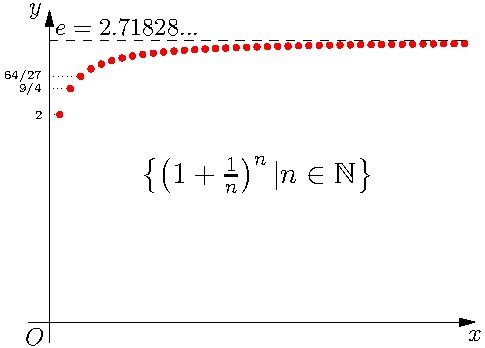
\includegraphics[width=0.5\textwidth]{./images/ch01/e-notin-N.pdf}
	\caption{有理数列$\left\{\left(1+\df1n\right)^n\right\}$构成的集合
	上确界为$e\notin\mathbb{Q}$}
	\label{fig:2.1}
\end{figure}
根据常用极限\ps{$e=\lim\limits_{n\to\infty}\left(1+\df1n\right)^n$}
不难看出$e=\mathrm{sup}A$,但$e\notin\mathbb{Q}$,
故有理数集不满足连续性公理。\fin

又比如这样一个例子:$A=\{x\in\mathbb{Q}|x\geq 0,\;x^2<2\}$,显然,
$\mathrm{sup}A=\sqrt2\notin\mathbb{Q}$。
\fi

\bs
{\bf 思考:}任给一个实数,如何构造一个有理数集合,使得该实数恰好为
该有理数集合的上(下)确界?

\ifhint
答:方法很多,以下给出其中一种。

设该实数为:
$$a=A.a_1a_2a_3\ldots a_n\ldots,$$
其中$A$为整数,$a_i(i=1,2,\ldots)$均为$0,1,\ldots,9$之中的
个位数。

定义如下的两个集合:
$$A_1=\left\{A.a_1a_2\ldots a_n-\frac1n
\Big|n\in\mathbb{Z}^+\right\},
\quad
A_2=\left\{A.A.a_1a_2\ldots a_n-\frac{\sqrt2}n\Big|
n\in\mathbb{Z}^+\right\},$$
因为有理数与有理数的和仍为有理数,而有理数与无理数的和必为无理数,
故易知$A_1\subset\mathbb{Q}$,$A_2\subset\mathbb{R}-\mathbb{Q}$。
此外,容易验证
$$\sup A_1=\sup A_2=a.$$
\fin
\fi

\begin{shaded}
	{\bf 开集与闭集}
	
	集合$A\subset\mathbb{R}$为{\bf 开集},是指:对任意$x\in A$,
	均存在$\delta>0$,使得
	$U(x,\delta)\subset A.$
	
	集合$A\subset\mathbb{R}$为{\bf 闭集},是指其补集
	$\bar{A}=\mathbb{R}-A$为开集。
	
	例如:所有的开区间都是开集,所有的闭区间为闭集;
	我们通常{\it 约定空集$\phi$既是开集又是闭集},
	因此{\it 实数集$\mathbb{R}$既是开集又是闭集}。
	
	点$a$称为集合$A$的{\bf 内点},是指:存在$\delta>0$,
	使得$U(a,\delta)\subset A$。显然开集中的点均为其内点!
	
	点$a$称为集合$A$的{\bf 外点},是指:存在$\delta>0$,
	使得$U(a,\delta)\cap A=\phi$,
	或者说$a$为$A$的补给的内点。
	
	点$a$称为集合$A$的{\bf 边界点},是指$a$既不是$A$的内点,
	也不是$A$的外点,或者说
	对任意的$\delta>0$,$U(a,\delta)\cap A\ne\phi$。
	
	显然,闭集可以视为其最大开子集和其所有边界点的并。
	
	\bs

	\egz 指出以下集合哪些是开集,哪些是闭集?
	\begin{enumerate}[(1)]
	  \setlength{\itemindent}{1cm}
	  \item $\{1,2,3,5\}$\hfill({\it 闭})
	  \item $U_0(1,3)$\hfill({\it 开})
	  \item 自然数集\hfill({\it 闭})
	  \item 有理数集\hfill({\it 既非开又非闭})
	  \item 无理数集\hfill({\it 既非开又非闭})
	  \item $\left\{\left(1+\frac
	  1n\right)^n|n\in\mathbb{N}\right\}+\{e\}$\hfill({\it 闭})
	\end{enumerate}
\end{shaded}

\subsection{映射}

映射通常被定义为,事物之间“一对一”或“多对一”的依赖关系。更形象地说,可以将
映射视为一种输入输出过程,“一对一”或“多对一”保证了
一个输入只能得到一个特定的输出,因此结果是{\it 无歧义}
\ps{无歧义是保证数学论证简明性的一个常见的要求}
的。从这个意义上说,对于映射的这种定义方式也是一种{\it 约定}。
由集合$A$到$B$的映射$f$一般记为:
$$f:A\mapsto B \quad\mbox{或}\quad y=f(x),\;x\in A,y\in B$$

{\it 映射的三要素:}定义域、值域、对应关系,任何一项不明确都不足以确定一个函数,或者说,
两个映射在这三方面有一点不同,则应视为不同的映射。
\ps{之所以有时候只关心定义域和对应关系,前提是默认假设映射为满射}

{\bf 函数}通常是指数集之间的映射。有时也推广到高维的数集,例如
$$z=x^2+y^2,\;(x,y)\in\mathbb{R}^2.$$

\egz 假设下列函数均取{\it 自然定义域}
\ps{即在$\mathbb{R}$中可取到的最大定义范围},
且均为满射,指出其中哪些是完全相同的?
$$x,\quad |x|,\quad e^{\ln x},\quad \ln(e^x),\quad \sqrt{x^2},\quad
\frac{x^2-4}{x-2}-2,$$
$$\sin(\arcsin x),\quad \arcsin(\sin x), \quad \tan(\arctan x)$$

与映射和函数相关的概念还有{\bf 单射、满射、一一映射(双射)},不再一一赘述。

\begin{shaded}
	\pss{\centering
	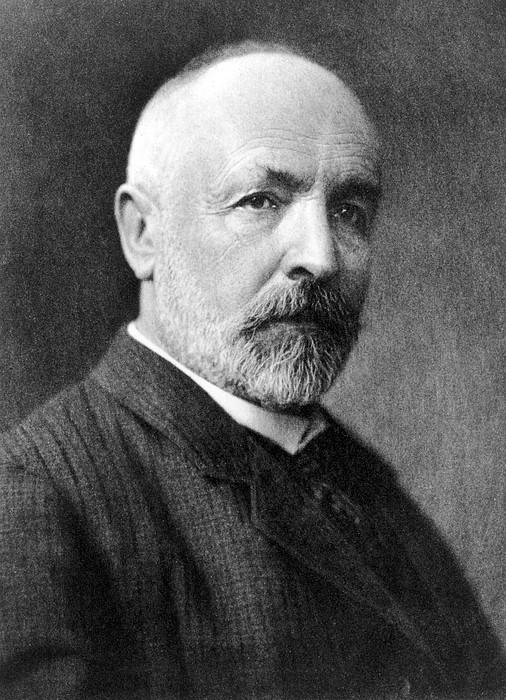
\includegraphics[width=0.7\marginparwidth]{./images/ch01/Cantor.jpg}\\
	\href{https://en.wikipedia.org/wiki/Georg_Cantor}{G. Cantor(1845-1918)}
	}
	{\bf 一一映射与无穷集合}

	考虑一个问题:如何比较两个集合中元素的个数?

	一般来说,我们称两个元素个数相同的集合为{\it 等势}的。对于
	元素有限的集合来说,判断两个集合是否等势也很容易的。困难在于
	如何判定两个元素个数不是有限的集合等势!

	Cantor的一大贡献就是给出了这个问题目前最广为接受的方法,或者说,
	他实际上给出了集合等势的严格定义:
	如果存在集合$A$和$B$之间的一一映射,则$A$和$B$是{\bf 等势}的。
	紧接着,他证明了一系列重要的集合之间的等势关系。
	
	\bs

	\egz 以下集合两两等势吗,为什么?
	({\baa 正确的命题须给出证明,错误的则只需举出反例})
	\begin{enumerate}[(1)]
	  \setlength{\itemindent}{1cm}
	  \item 自然数与正偶数({$\surd$})
	  \item 自然数与整数({$\surd$})
	  \item 自然数与有理数({$\surd$})
	  \item 区间$(0,1)$中的实数与$\mathbb{R}$中({$\surd$},例如:$y=\df1{e^x+1}$)
	  \item 自然数与实数({$\times$})
	\end{enumerate}
	
	\bs
	提示:一个集合与自然数集等势,等价于这个集合中的所有数可以不重复地
	排成一列,形象地说,就是可以把这个集合中所有的数一个个地数完而没有任何重复
	与遗漏。

	例如要证明整数集与自然数集等势,显然只需这样来排列整数集:
	$$0,1,-1,2,-2,3,-3,4,-4,\ldots,$$
	很容易看出这样的排列是既没有遗漏也没有重复的,
	事实上等于给出了从自然数集到整数集的一一映射。
	显然要证明自然数集和正偶数集等势也是一样的容易。
	
	\bs
	(3)\;参照上面的作法,要证明自然数集与有理数集等势,
	也只需要考虑能否找到一种方式
	将所有的有理数排成一列,既不重复也不遗漏。
	参考图\ref{fig:1-2},我们可以先说明所有的正有理数
	可以排成一列:
	$$1,2,\df12,3,\df13,4,\df32,\df23,\df14,5,\df15,6,\df52,
	\df43,\df34,\df25,\df16,\ldots,$$
	从图上不难看出,这个排列事实上给出了从自然数集到正有理数集的一一映射。
	接下来,在其中逐个插入对应的负有理数,即可得到从自然数集到有理数集的
	一一映射。
	
	{\bf 思考:}能否证明$\mbb{Z}$和$\mbb{Z}^2$是等势的?任意给定某个$n$,
	$\mbb{Z}$和$\mbb{Z}^n$也等势吗?$\mbb{Q}$和$\mbb{Q}^n$呢?
	$\mbb{R}$和$\mbb{R}^n$呢?
	
	(5)\;我们只需证明不存在自然数集到区间$(0,1)$的一一
	映射即可。
	
	反证法(据说这是Cantor最初的证明方法):假设存在自然数集到$(0,1)$的
	一一映射,这意味着$(0,1)$中所有的数可以排成一个数列,没有重复也没有遗漏,
	设其中第$i$个数表示为
	$$a_i=a_{i1}a_{i2}a_{i3}a_{i4}\ldots,$$
	其中$a_{ij}(j=1,2,\ldots)$都是$0$到$9$之间的个位整数。
	
	接下来,我们构造一个新的数
	$$a_*=a_{*1}a_{*2}a_{*3}a_{*4}\ldots,$$
	其中$a_{*j}(j=1,2,\ldots)$也都是$0$到$9$之间的个位整数,同时满足
	$$a_{*j}\ne a_{jj},\; j=1,2,3,\ldots.$$
	
	从$a_*$的构造特点上,我们可以得出如下两个结论:
	\begin{enumerate}[(i)]
	  \setlength{\itemindent}{1cm}
	  \item $a_*\in(0,1)$,
	  \item $a_*\ne a_i,\;i=1,2,3,\ldots$
	\end{enumerate}
	由于根据我们的假设,数列$\{a_i\}$中已经不多不少地包含了$(0,1)$中所有的数,因此
	以上第二条恰好说明$a_*\notin(0,1)$,这就出现了矛盾。从而可以断言
	假设错误,也就是说,不存在自然数集到$(0,1)$的一一映射,因此二者
	不等势,最终得到结论自然数集与实数集也不等势。\fin 
	
	\bs
	上面这些结论反映出一个有趣的现象,就是有些集合可以和自己的真子集建立起
	一一映射。	Cantor敏锐地抓住了这一点,并认为应该是{\it 无穷集合}的本质
	特征,进而第一次给出了无穷集合的定义
	\begin{tcolorbox}
		{\bf 无穷集合:}可以和自身的某个真子集建立起一一映射的集合。
	\end{tcolorbox}
	历史上,Cantor曾被人称为“{\it 数学史上最富于想象力的最具争议的人物之一}”、
	拥有“{\it 对于提出深刻的问题以及不时探索始料未及的解法以至寻求非正统答案的天赋}”。
	他的名言也是信条是“{\it 数学的本质在于它超然的自主性}”。
\end{shaded}	

\begin{figure}[tbp]
	\centering
	\includegraphics[width=0.65\textwidth]{./Images/Ch01/Q-Counting.pdf}
	\caption{有理数表:对应位置的数字为有理数$\df pq$。
	按照箭头所指的顺序,\\
	从左上到右下可以在表中找到所有的正有理数,灰色背景的是重复出现的数字}
	\label{fig:1-2}
\end{figure}

\subsection{函数}
	
函数是微积分研究的基本对象,不同于中学阶段以对函数值的讨论和计算为重点,
微积分更关注函数的变化特征(如导数与高阶导数、曲率)与整体性质(如连续性、
定积分)。

{\bf (一元)函数}就是由实数集到实数集的映射,可记为
$$f:D\mapsto\mathbb{R},\;(D\subset\mathbb{R})$$
或
$$y=f(x),\quad (x\in D\subset\mathbb{R},y\in\mathbb{R}).$$

{\bf (一元函数的)函数图像}是如下的集合:
\ps{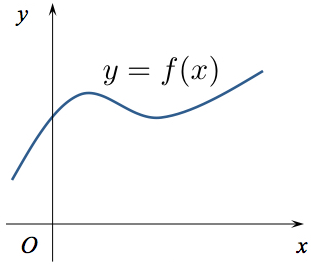
\includegraphics[width=\marginparwidth]{./images/Ch01/C_fx.jpg}}
$$G=\{(x,f(x))\in\mathbb{R}^2|x\in D\}.$$

{\bf 思考:}一元函数的图像是否一定是平面内的一条曲线?

\ifhint
答:不一定,有可能是完全不连续的形态,不构成任何一段曲线。例如:
稍后将要介绍的Diriclet函数(在有理数点和无理数点上分别取值$0$和$1$)。
\fi

\begin{shaded}
	在微积分这门课中,我们还将学习:

	{\it 多元($n$元)函数}, 形如
	$$f:D\to\mathbb{R},\quad D\in\mathbb{R}^n\quad
	\mbox{或}\quad y=f(\bm{x}),\;\bm{x}\in D\subset\mathbb{R}^n$$

	{\it ($n$维)向量值函数,}形如
	$$\bm{f}:D\to\mathbb{R}^n,\quad, D\in\mathbb{R}\quad
	\mbox{或}\quad \bm{y}=\bm{f}(x),x\in D\subset\mathbb{R},
	\bm{y}\in\mathbb{R}^n$$
		
	{\bf 思考:}二元函数和三维的向量值函数可以表示怎样的几何对象?
	\ifhint
	\pss{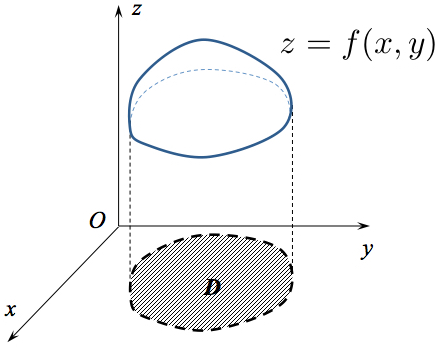
\includegraphics[width=\marginparwidth]{./images/Ch01/S_fxy.jpg}}
	二元函数的图像一般可以表示为三维空间中的一个曲面,而三维的向量值
	函数则对应于三维空间中的一条曲线。
	\fi
\end{shaded}
	
{\bf 思考:}平面曲线与一元函数具有一一对应关系吗?空间曲面和二元函数呢?

\ifhint
答:不是的,例如圆$x^2+y^2=1$如果写成一元函数形式,需要至少两个函数
$y=\pm\sqrt{1-x^2}$。空间曲面和二元函数的关系与之类似,例如空间球面
$x^2+y^2+z^2=1$也至少需要写成两个$z$关于$x,y$的二元函数
$z=\pm\sqrt{1-x^2-y^2}$。
	
由于以上问题的存在,为了表示平面曲线(空间曲面),我们会用到其他一些的曲线方程,
例如:单位圆的方程也可以写为:
\begin{itemize}
	\item {\it 隐函数方程}:$x^2+y^2=1$;
	\item {\it 参数方程}:$(x,y)=(\cos t,\sin t),\quad t\in[0,2\pi]$;
	\pss{关于参数方程和极坐标方程的介绍,参见KD教材1.3节}
	\item {\it 极坐标方程}:$\rho=1,\theta\in[0,2\pi]$。
\end{itemize}
\fi
	
\subsubsection{函数的运算}

函数运算是由基本函数构造更复杂函数的常用手段,常见的函数运算包括:
\begin{enumerate}
  \setlength{\itemindent}{1cm}
  \item {\it 四则运算:}$+,-,\cdot,/$;
  \item {\it 复合运算:}函数的复合运算就是
  中间变量的代入过程,可表示为:$(f\circ g)(x)=f(g(x))$;
  \item {\it 逆运算:}也就是求反函数。
  \ps{函数求逆(反函数)的前提:$f$必须为一一映射}。
\end{enumerate}

\bs
{\bf 思考:}$y=f(x)$和$x=f^{-1}(y)$的图形的关系是怎样的?

\ifhint
答:相同!
\fi

\subsubsection{函数的简单性质}

今后的讨论中,为了书写方便,我们约定可使用如下的简写符号:
\begin{tcolorbox}[colback=white!90!black]
	{\bf 常用的简写符号:}约定用于数学推导中一些常用文字的书写替代,汉英通用
	\begin{itemize}
	  \item[{\b$\bm{\forall}$}]  \quad 任意 (for all, arbitrary)
	  \item[{\b$\bm{\exists}$}] \quad 存在 (exist)
	  \item[{\b$\bm{\Rightarrow}$}] \quad 推出 (deduce, imply)
	  \item[{\b$\bm{\Leftrightarrow}$}] \quad 等价、当且仅当 (equivalent, if and only if)
	  \item[{\b$\bm{\to}$}] \quad 趋于 (approach)
	\end{itemize}
\end{tcolorbox}

{\bf 1.有界性}

设$I\subset\mathbb{R}$,$f(x)$在$I$上有定义,若集合
$\{f(x)|x\in I\}$有界,
则称{\bf $f(x)$在$I$上有界}或{\bf $f(x)$是$I$上的有界函数}。
\ps{函数有界就是其值域有界}

\bs
\egz 判断以下函数在其定义域上的有界性\ps{参见图\ref{fig:sinFigures}}

\quad(1)\;$y=x\sin x$,\hspace{5em} (2)\;$y=\df{\sin x}x$,
\hspace{5em} (3)\;$y=\sin\df1x$

\begin{figure}[h]
	\centering
	\begin{subfigure}[t]{0.45\textwidth}
		\centering
		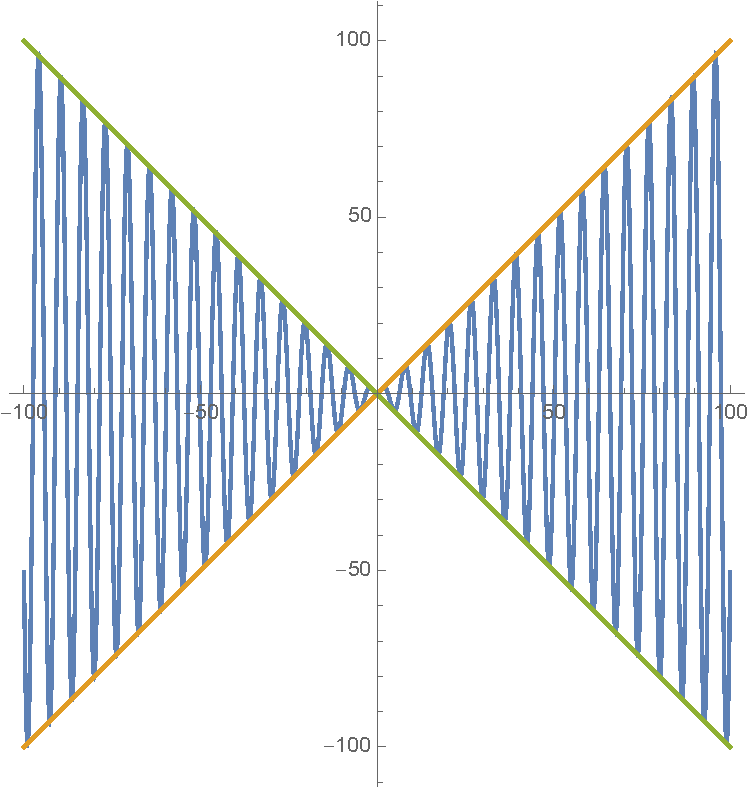
\includegraphics[width=\textwidth]{./images/Ch01/xsinx.pdf}
		\caption{$y=x\sin x$}
	\end{subfigure}
	\begin{subfigure}[t]{0.45\textwidth}
		\centering
		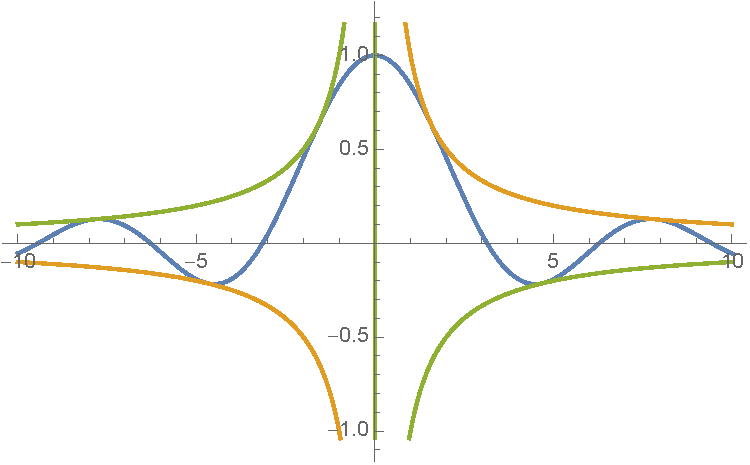
\includegraphics[width=\textwidth]{./images/Ch01/1xsinx.pdf}
		\caption{$y=x\sin x$}
	\end{subfigure}

	\begin{subfigure}[t]{0.45\textwidth}
		\centering
		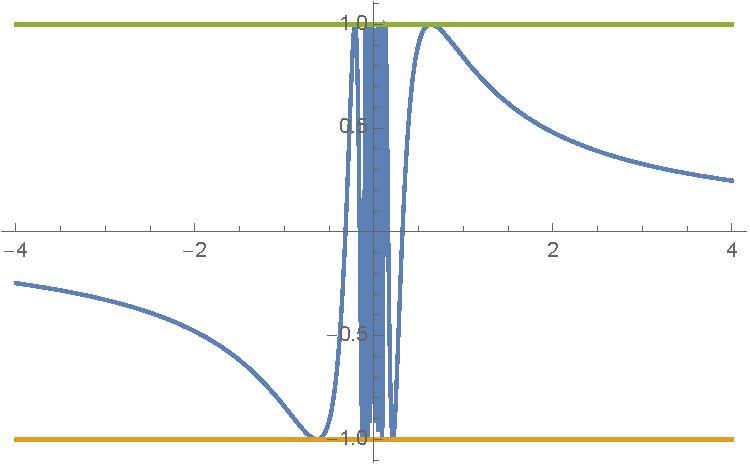
\includegraphics[width=\textwidth]{./images/Ch01/sin1x.pdf}
		\caption{$y=x\sin x$}
	\end{subfigure}
	\caption{\exNo 图(建议熟练掌握)}
	\label{fig:sinFigures}
\end{figure}

\begin{shaded}
	{\bf 反(否)命题的写法}	

	有时候,我们已经需要给出某个命题的反(否)命题。根据一阶逻辑的基本
	法则,可以得到如下的替换规则:逐个对命题中的如下文字进行相互替换
	\begin{enumerate}
	  \setlength{\itemindent}{1cm}
	  \item {\b “任意”与“存在”}
	  \item {\b “$\geq(\leq)$”与“$<(>)$”}
	  \item {\b “和”与“或”}
	\end{enumerate}
	
	\bs
	以函数的有界性为例,其否命题为函数无界。
	\begin{tcolorbox}
		{\it $f(x)$在区间$I$上有上界}:{\b\it 存在}$M\in\mathbb{R}$,对
		{\b\it 任意}$x\in I$,有$f(x){\b \leq} M$。
		
		{\bf $f(x)$在区间$I$上无上界}:对{\b\it 任意}$M\in\mathbb{R}$,
		{\b\it 存在}$x_M\in I$,使得$f(x_M){\b >}M$。
	\end{tcolorbox}
	
	\bs
	\egz 用以上关于函数无上界的定义,证明$y=x\sin x$无界。
	
	注:所谓{\it 用定义证明}函数的性质,就是验证该函数满足这个定义中的命题。
	
	证:对任意$M\in\mathbb{R}$,
	令$x_M=\left(\left[\df{M}{2\pi}\right]+1\right)
	\cdot2\pi+\df{\pi}2$(其中$[x]$为{\it 下取整函数},表示不大于$x$的最大整数,
	显然$[x]\leq x<[x]+1$),	则有
	$$x_M>\df{M}{2\pi}\cdot2\pi+\df{\pi}2>M,
	\quad\mbox{且}\quad \sin x_M=1,$$
	故
	$$x_M\sin x_M=x_M>M.$$
	从而根据函数无上界的定义,可知该函数无上界,从而无界。\fin
	
	注:有界是指既有上界又有下界,故无上界或无下界都可推出无界!
	
	\bs
	\egz 证明:$f(x)=\df{\cos x}x$无界。
	
	证:对任意$M>0$,令$x_M=\min\left\{\df{\pi}4,\df1{2M+1}\right\}$,
	由于$x_M<\pi/3$时,$\cos x_M>\df12$,故
	$$f(x_M)>\df1{2x_M}>\df1{2\df1{2M+1}}=M+\df12>M,$$
	于是由定义可知,$f(x)$无界。\fin
\end{shaded}		

{\bf 2.单调性}

设$f:I\mapsto\mathbb{R}$,若对$\forall x_1,x_2\in I$,总有
$$x_1<x_2\Rightarrow f(x_1)\leq f(x_2)$$
则称{\bf $f(x)$在$I$上单调递增}(若不等式中的等号总是无法成立,则称为
{\bf 严格单调递增})
	
\bs
\egz 证明函数$f(x)=x+\sin x$严格单调递增。
\ps{\centering
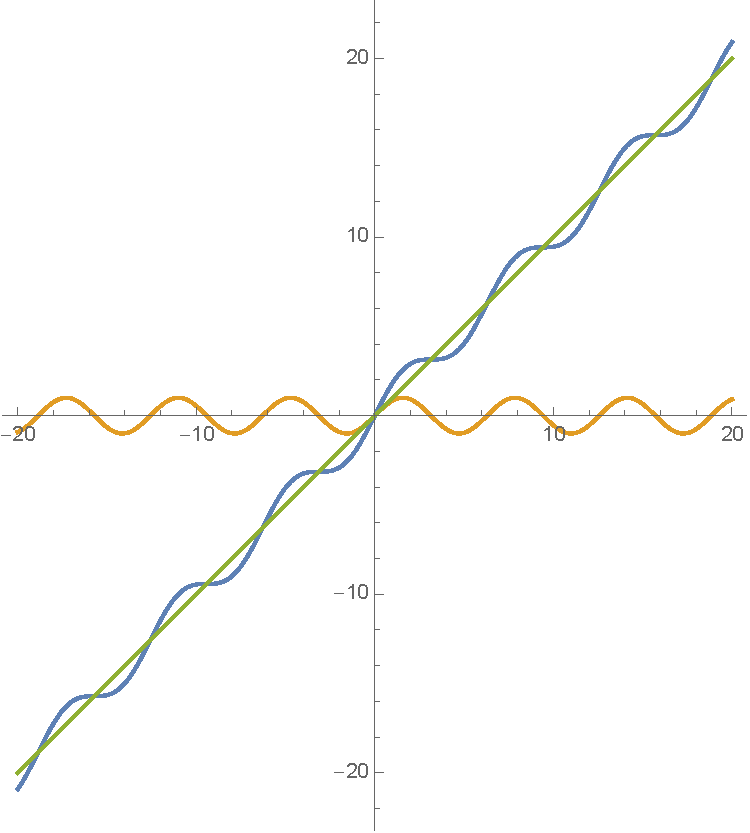
\includegraphics[width=\marginparwidth]{./images/ch01/xpsinx.pdf}\\
$y=x+\sin x$和$y=\sin x$}

证:该函数的定义域为$\mathbb{R}$,任取$x_1,x_2\in\mathbb{R}$,则
$$f(x_2)-f(x_1)=(x_2-x_1)+2\sin\df{x_2-x_1}{2}\cos\df{x_2+x_1}{2}.$$

若$x_2-x_1>2\pi$,则由$\sin\df{x_2-x_1}{2}\cos\df{x_2+x_1}{2}\geq -1$,可得
$$f(x_2)-f(x_1)>(x_2-x_1)-2>2\pi-2>0;$$

若$0<x_2-x_1<2\pi$,注意到$|\sin x|<x\;(x>0)$,则有
$$f(x_2)-f(x_1)>(x_2-x_1)-2\left|\sin\df{x_2-x_1}{2}\right|
>(x_2-x_1)-2\df{x_2-x_1}{2}=0.$$

综上所述,对任意$x_2>x_1$,恒有$f(x_2)-f(x_1)>0$,故$f(x)$严格单调递增。
\fin

\bs
{\bf 思考:}严格单调的函数一定是一一映射,故一定存在反函数。如果反之,
存在反函数的函数一定会严格单调吗?

\ifhint
答:反之不成立。例如函数
\ps{\centering
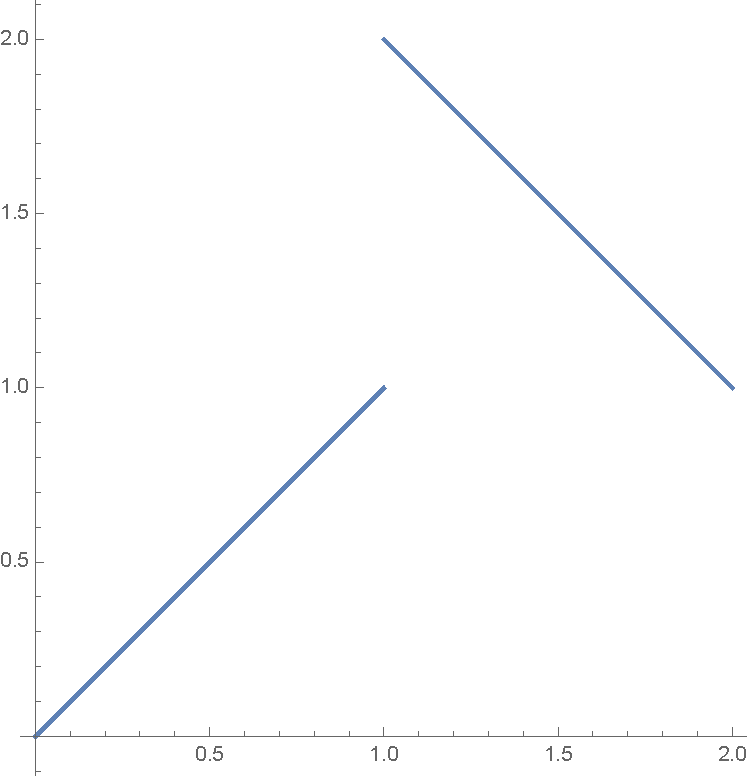
\includegraphics[width=\marginparwidth]{./images/ch01/pswsRef.pdf}
可逆但不整体单调}
$$f(x)=\left\{\begin{array}{ll}
	x,&0<x<1;\\
	3-x,&1\leq x<2
\end{array}\right.$$
的反函数就是其自身,但在定义域上不是单调的。\fin

请进一步思考:以上反例中的函数在每个连续的区间(例如$(0,1)$)
上仍然是严格单调的,这是函数存在反函数的必要条件吗?换句话说,
是否存在某个函数存在反函数,却在任意的区间上都不单调呢?
\fi

\bs
{\bf 思考:}若对任意$x_1,x_2$,总有
$$[f(x_2)-f(x_1)](x_2-x_1)\leq 0,$$
可以推断$y=f(x)$具有何种性质?

\ifhint
答:$y=f(x)$单调递减。
\fi

\bs

{\bf 3.奇偶性}

设函数$f:D\mapsto\mathbb{R}$,{\bf 称$f(x)$为偶(奇)函数},是指:
对任意$x\in D$,有$f(-x)=f(x)\quad(f(-x)=-f(x))$

奇偶性是对称性的一种特例,由奇偶性的定义,很容易得到关于函数对称性的一些定义:

\bs
\egz 试给出如下性质的数学定义
\begin{enumerate}[(1)]
  \setlength{\itemindent}{1cm}
  \item 函数$y=f(x)$的图像关于$x=a$对称
  \dotfill$f(2a-x)=f(x)$
  \item 函数$y=f(x)$的图像关于点$(x_0,y_0)$对称
  \dotfill $f(2a-x)=2f(a)-f(x)$
\end{enumerate}

\bs
{\bf 思考:}$f(x)=g(a-x),\;(x\in\mathbb{R})$有什么几何意义?

\ifhint
答:$f(x)$和$g(x)$的图像关于$x=a/2$对称!例如:$\sin x
=\cos(\pi/2-x)$,函数$y=\sin x$和$y=\cos x$图像关于$x=\pi/4$对称。
\fi

\bs
\begin{thx}
	{\bf 定理:}任意一个定义在对称区间上的函数均可以表示为一个偶函数和一个奇函数的和,即
	$$f(x)=\df{f(x)+f(-x)}{2}+\df{f(x)-f(-x)}{2}.$$
\end{thx}
例如:
$$e^x=\df{e^x+e^{-x}}2+\df{e^x-e^{-x}}2$$

\bs
{\bf 4.周期性}

设函数$f:\mathbb{R}\to\mathbb{R}$,
称{\bf $f(x)$为周期函数},是指: 存在$T>0$,
使对任意$x\in\mathbb{R}$,有
$f(x+T)=f(x)$。
满足以上性质的最小正数$T$称为$f(x)$的{\bf 最小正周期}。
		 
显然,若$T$为$f(x)$的一个周期,则任意$n\in\mathbb{Z}$和
任意$x\in\mathbb{R}$,总成立
$$f(x+nT)=f(x).$$

\subsubsection{常用函数}

{\bf 1.符号函数}

$$\mathrm{sgn}\,x =\left\{
\begin{array}{rl}
-1,\;&x<0 \\
0,\;&x=0 \\
1,\;&x>0
\end{array}
\right.$$
显然,
$$|x|=x \cdot\mathrm{sgn} x$$
	
{\bf 2.(下)取整函数(阶梯函数)}

$$y=\left[ \,x\, \right]$$
其中$[\,x\,]$表示小于等于$x$的最大整数。容易得到如下的性质:
\begin{enumerate}[(1)]
  \setlength{\itemindent}{1cm}
  \item $[x]\leq x<[x]+1$
  \item $[x+1]=[x]+1$
\end{enumerate}

\bs
利用取整函数,可以构造出一些简单但在工程实践中非常重要的函数,例如:
{\it 方波}和{\it 三角波}\ps{经常也写为$y=\df1{\pi}\arccos(\cos\pi x)$}:
\begin{figure}[h]
	\centering
	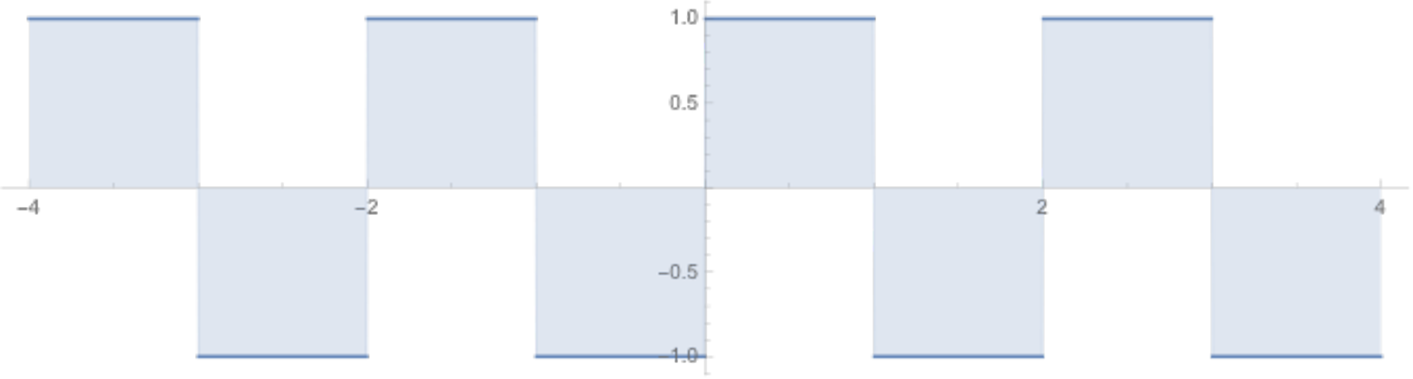
\includegraphics[width=0.7\textwidth]{./images/ch01/rectWave.pdf}
	\caption{方波$y=(-1)^{[x]}$}
	\label{fig:rectWave}
\end{figure}
\begin{figure}[h]
	\centering
	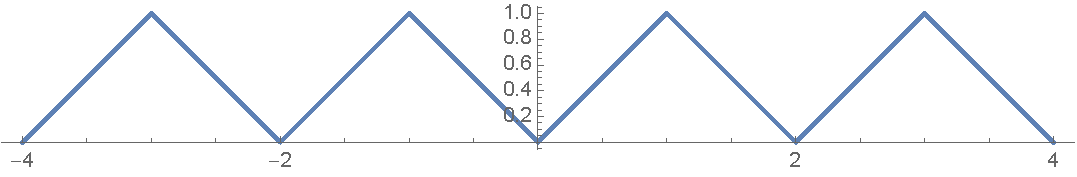
\includegraphics[width=0.7\textwidth]{./images/ch01/triWave.pdf}
	\caption{三角波$y=\left|x-2\left[\df x2\right]\right|$}
	\label{fig:triWave}
\end{figure}

\bs

{\bf 3.Dirichlet函数}

  $$\bm{D}(x) =\left\{
  \begin{array}{ll}
  	1,\;& x\in\mathbb{Q} \\
  	0,\;& x\notin\mathbb{Q}
  \end{array}
  \right.$$

  {\bf 性质:}\ps{将在后续章节中加以证明}
  \begin{enumerate}[(1)]
    \setlength{\itemindent}{1cm}
    \item $D(x)$在实数轴上处处无极限;
	\item $D(x)$在实数轴上处处不连续;
	\item {\it 仅在$x=0$这一点连续的函数:}$y=xD(x)$;
	\item {\it 仅在$x=0$这一点可导的函数:}$y=x^2D(x)$。
  \end{enumerate}

$D(x)$的最后这两个性质有些违反我们的直觉,因为现实中并不存在什么曲线
能够只在一个点连续或者只在一个点处光滑!这真是数学自身的
特异指出,为了确保自身的严谨,而适当地“牺牲”了一些与直觉
一致的东西。

\bs

{\bf 4.Riemann函数} \ps{也被称为“直尺函数”,最初由卡尔$\cdot$托梅提出}:
设$x\in[0,1]$,
  $$\bm{R}(x) =\left\{
	\begin{array}{ll}
	1,\;&x=0\\
	\displaystyle\frac 1q,\;&x=\displaystyle\frac pq,\,p,q\mbox{互素}\\
	0,\;&x\notin\mathbb{Q}
	\end{array}
  \right. $$
$R(x)$和$D(x)$一样,也有许多“反直觉”的地方,例如:
\begin{itemize}
	\item 对任意$x_0\in[0,1]$, $\lim\limits_{x\to x_0}R(x)=0$;
	\item $R(x)$在{\it 所有的无理数点处连续,在所有的有理数点处不连续};
	\item $R(x)$是Riemann可积的。
\end{itemize}

\bs

{\bf 5.初等函数}

{\bf 初等函数}
\pss{注意两个重要的限定词:
\begin{itemize}
	\item 有限次
	\item 一个式子
\end{itemize}
因此,通常来说,分段定义的函数不能算初等函数
}
是指由常数和{\it 基本初等函数}经过
{\it 有限次}的四则运算和{\it 有限次}的函数复合
步骤所构成并可用{\it 一个式子}表示的函数。

{\bf 基本初等函数}包括以下五类:
\begin{enumerate}
  \setlength{\itemindent}{1cm}
  \item {\bf 幂函数:} $y=x^a,\; (a\in\mathbb{R})$
  \item {\bf 指数函数:} $y=a^x,\; (a>0,a\ne 1)$
  \item {\bf 对数函数:} $y=\log_ax,\; (a>0,a\ne 1)$
  \item {\bf 三角函数:} $\sin x, \,\cos x,\, \tan x, \,\cot
  x,\, \sec x,\, \csc x$
  \item {\bf 反三角函数} :
  $\arcsin x, \,\arccos x, \arctan x,\ldots$
\end{enumerate}

{\baa 学习要求:熟练掌握五类基本初等函数的定义、图像、基本性质、
各种运算公式(例如:三角函数的和差化积、积化和差、半(倍)角公式、
万能公式;反三角函数的定义域、值域、单调性;一些常用的不等式,
如$e^x-1>x>\ln(x+1)\;(x>0)$、平均值不等式、
$\sin x<x<\tan x\;(x>0)$等等。}

\bs
{\bf 问:}$\arcsin x$和$\arccos x$的定义域值域有何不同?

答:因为三角函数都是周期函数,所以只能选择其周期内某个单调区间上
的一段函数来定义反函数。在选择这样的区间时,注意掌握两个原则:
(1)尽可能靠近原点;(2)有限考虑对称区间或原点右侧的区间。
常用的反三角函数的图像见图\ref{fig:triFunc}。

\begin{figure}[h]
	\centering
	\begin{subfigure}[t]{0.45\textwidth}
		\centering
		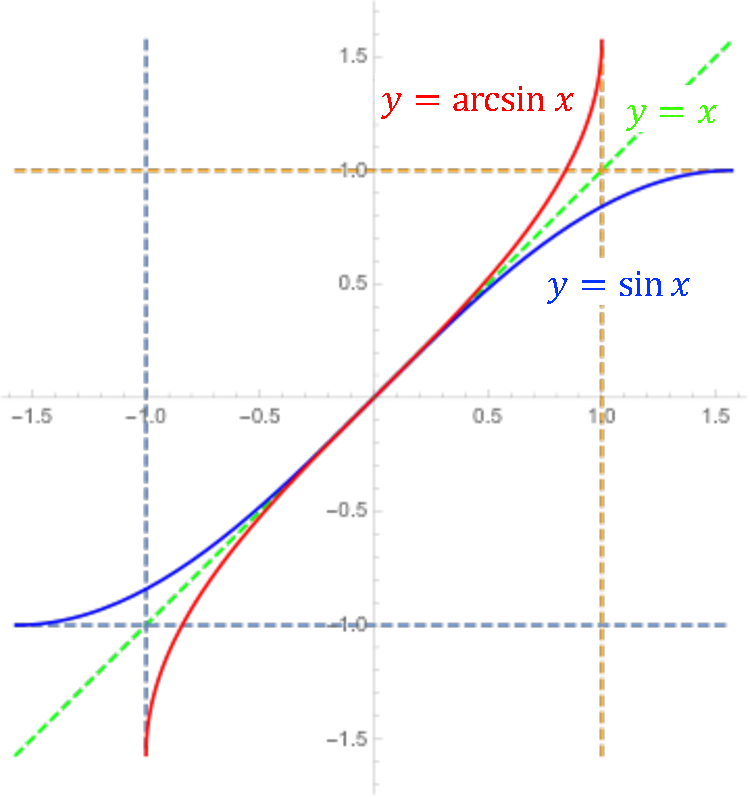
\includegraphics[width=\textwidth]
		{./Images/Ch01/sin-Arcsin.pdf}	
		\caption{$\sin x$与$\arcsin x$的图像}
	\end{subfigure}
	\begin{subfigure}[t]{0.45\textwidth}
		\centering
		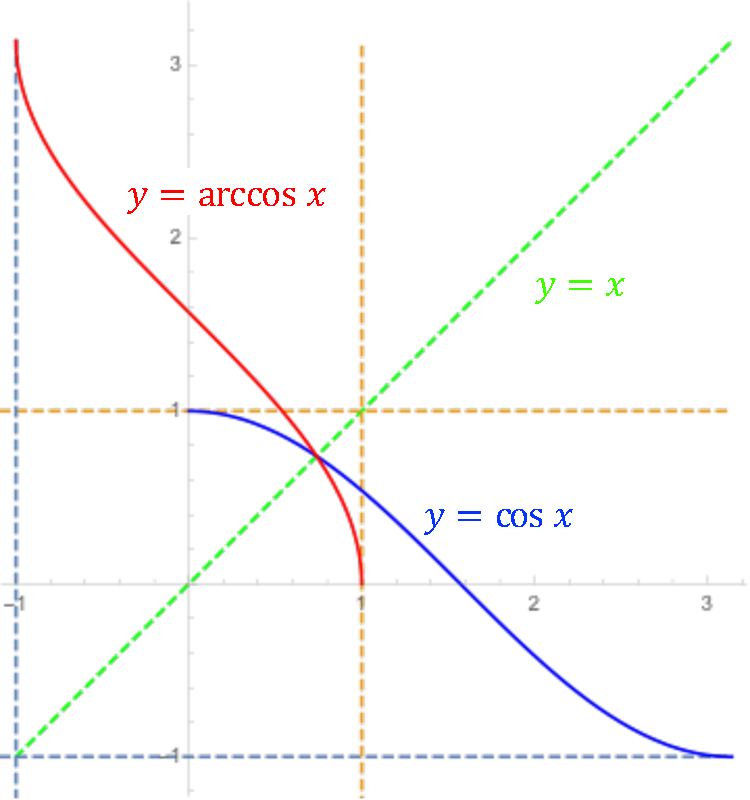
\includegraphics[width=\textwidth]
		{./Images/Ch01/cos-Arccos.pdf}	
		\caption{$\cos x$与$\arccos x$的图像}
	\end{subfigure}

	\begin{subfigure}[t]{0.45\textwidth}
		\centering
		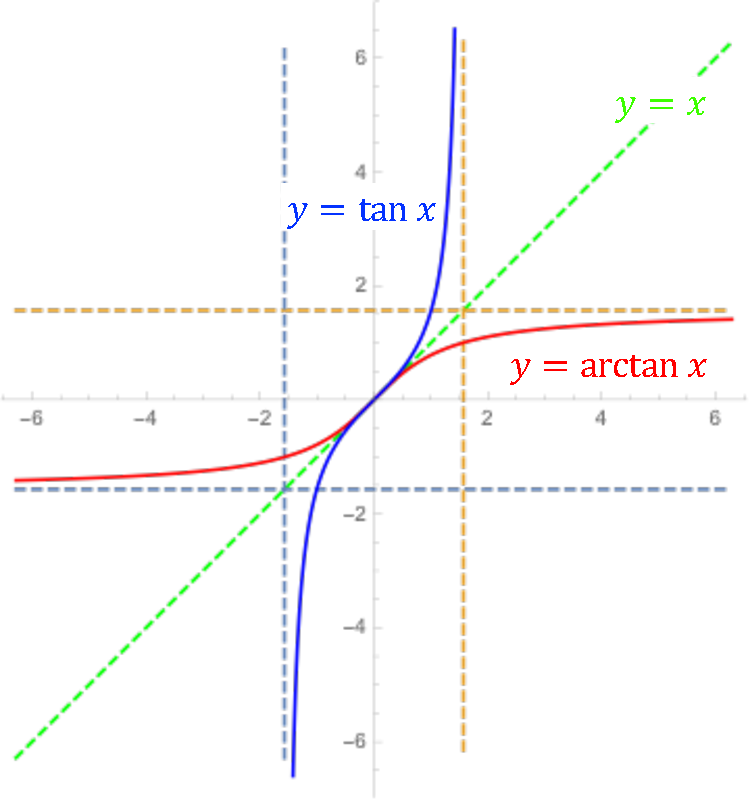
\includegraphics[width=\textwidth]
		{./Images/Ch01/tan-Arctan.pdf}	
		\caption{$\tan x$与$\arctan x$的图像}
		\label{subfig:arctan}
	\end{subfigure}
	\begin{subfigure}[t]{0.45\textwidth}
		\centering
		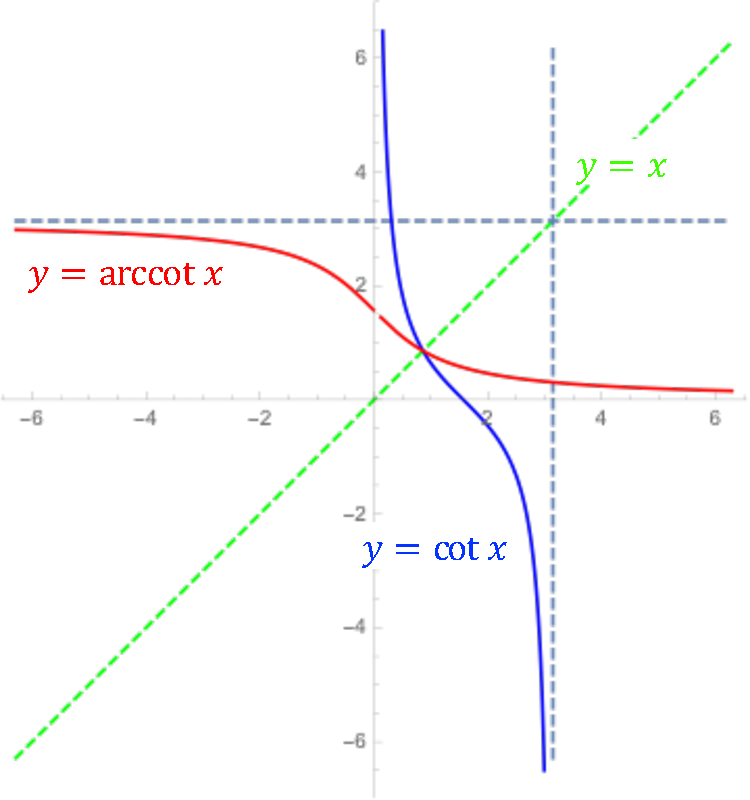
\includegraphics[width=\textwidth]
		{./Images/Ch01/cot-Arccot.pdf}	
		\caption{$\cot x$与$\mathrm{arccot} x$的图像}
	\end{subfigure}
	\caption{三角函数及其反函数的图像}
	\label{fig:triFunc}
\end{figure}

\bs
\egz 写出以下两个函数的表达式
$$\arcsin(\sin x),\quad \sin(\arcsin x)$$

解:$\sin(\arcsin x)=x$,其定义域为$[-1,1]$。

$\arcsin x$的值域为$[-\pi/2,\pi/2]$,因此作如下的讨论:

若$x\in[-\pi/2,\pi/2]$,则$\arcsin(\sin x)=x$;

若$x\notin[-\pi/2,\pi/2]$,则需要利用$\sin x$的性质
将$\sin x$化为某个$\sin(\bar x)$,其中$\bar x\in[-\pi/2,\pi/2]$,
且与$x$之间相差$\pi$的整数倍。进一步讨论:

若$\bar x-x=2n\pi$,其中$n$为整数,则$\sin\bar x=\sin x$,
此时
$$\arcsin(\sin x)=\arcsin(\sin\bar x)=\bar x=x+2n\pi.$$

若$\bar x-x=(2n+1)\pi$,其中$n$为整数,则$\sin(-\bar x)
=-\sin\bar x=\sin x$,
此时
$$\arcsin(\sin x)=\arcsin(\sin(-\bar x))=-\bar x=-(2n+1)\pi-x.$$

又注意到$\arcsin(\sin x)$显然是以$2\pi$
为周期函数,故以下只需给出其在一个周期上的
定义,其余部分按照周期进行复制即可。综上
$$\arcsin(\sin x)=\left\{\begin{array}{ll}
-x-\pi, & -\pi\leq x<-\pi/2,\\
x, & -\pi/2\leq x\leq\pi/2,\\ 
x+\pi, & \pi/2<x\leq\pi.
\end{array}\right.$$
其图像如下
\begin{figure}[h]
	\centering
	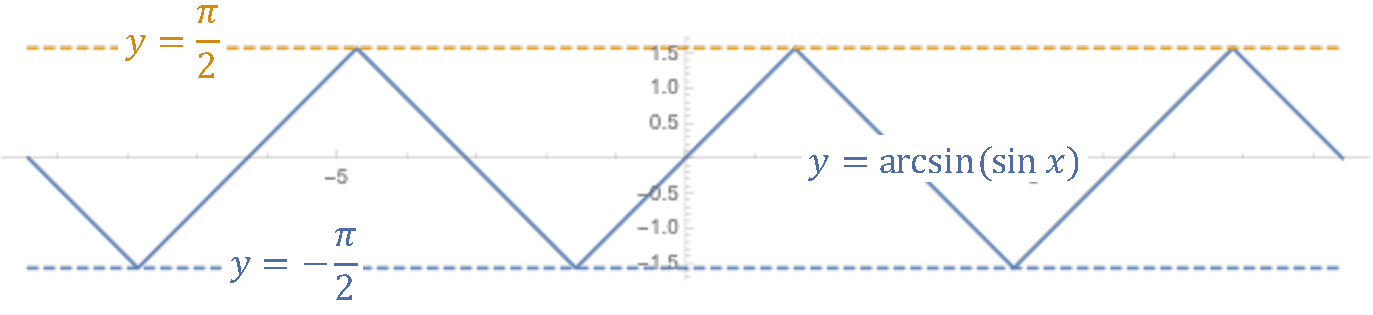
\includegraphics[width=0.7\textwidth]{./Images/Ch01/arcsin-sin.pdf}
	\caption{$\arcsin(\sin x)$的图像}
	\label{fig:arcsin-sin}
\end{figure}

类似地,我们可以得到$\arccos(\cos x)$的图像(如图\ref{fig:arccos-cos})\ps{请自行练习推导函数表达式}.
\begin{figure}[h]
	\centering
	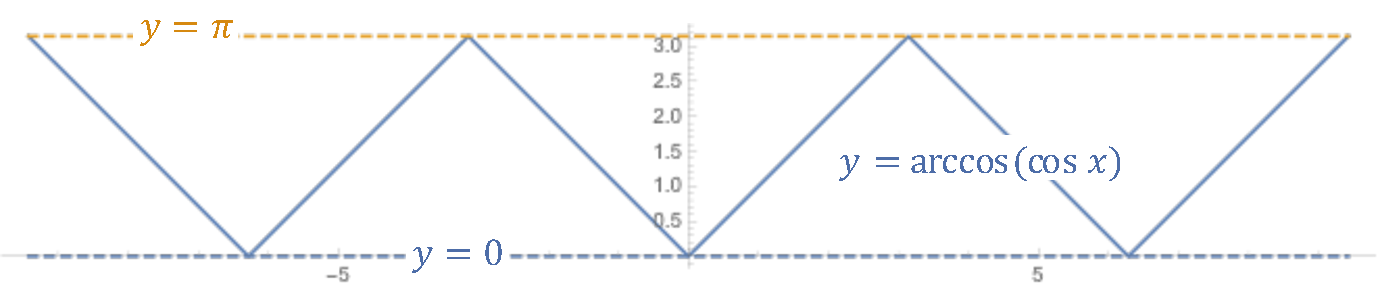
\includegraphics[width=0.7\textwidth]{./Images/Ch01/arccos-cos.pdf}
	\caption{$\arccos(\cos x)$的图像}
	\label{fig:arccos-cos}
\end{figure}
\fin

\egz 化简$\tan(\arcsin x),\;x\in(-1,1)$。

解:注意到
$$\tan x=\df{\sin x}{\cos x}=\df{\sin x}{\sqrt{1-\sin^2x}},$$
故
$$\mbox{原式}=\df x{\sqrt{1-x^2}},\quad x\in(-1,1).$$
\fin

{\bf 思考:}证明:$\pi=20\arctan\df17+8\arctan\df3{79}$.

\ifhint
提示:等式两边都除以$4$,然后取正切,再反复利用如下公式
$$\tan(A+B)=\df{\tan A+\tan B}{1-\tan A\tan B}.$$
\fi

\bs

{\bf 6.多项式函数}

多项式函数是一类非常“有用”的函数。之所以这么说,原因有二,一是因为
在所有的初等函数中,多项式函数是形式最简单的函数之一(只包含基本的
四则运算),因此任意给定自变量的值总可以直接计算出对应的函数值
(类似$e^x$,$\sin x$,$\arccos x$这样的函数都不行);
二是多项式函数具有很多重要的性质,使得它可以用来作为研究其他许多
函数的工具,甚至可以说,它是函数论中最重要、
最基本的工具也不为过。

一般的{\bf (一元$n$次)多项式函数}\ps{有理函数的次数也即其最高次幂
的项的次数}形如
$$P_n(x)=\sum_{i=0}^na_ix^i,
\quad (a_i\in\mathbb{R},a_n\ne 0,i=1,2,\ldots,n),$$
直观地说,它就是$x$的整数次幂的{\it 线性组合}。

多项式函数的基本性质包括\ps{这些性质的证明请参见高等代数有关的教材}:
  \begin{enumerate}[(1)]
    \setlength{\itemindent}{1cm}
    \item { $n$次多项式方程$P_n(x)=0$在$\mathbb{R}$上最多有$n$个根 (包含重根) ,在
    $\mathbb{C}$上有且仅有$n$个根(包含重根)};
    \item 设$x_i\in\mathbb{C}(i=1,2,\ldots,n)$为$P_n(x)=0$的全部根 ,则
    $$P_n(x)=a_n\prod_{i=1}^n(x-x_i)=a_n(x-x_1)(x-x_2)\ldots(x-x_n),$$
    \item 已知$P_n(x)$在$n+1$个点处的值, 可以唯一确定$P_n(x)$。
  \end{enumerate}

\bs

{\bf 7.有理函数}

有理函数也叫有理(分式)函数,形如:
$$f(x)=\frac{P(x)}{Q(x)}, \quad\mbox{其中}P(x),Q(x)\mbox{均为多项式函数}$$

和多项式函数类似,有理函数也是只要给定自变量的值就可以直接计算函数值的。

关于有理函数,需要我们掌握如下的性质:任意有理函数总可以化为一个多项式
函数和一个真分式(分子的次数比分母低的有理函数)的和。例如,使用
多项式的带余除法,我们可以得到
$$\frac{x^3+x^2-1}{x-1}=x^2+2x+2+\df{1}{x-1},$$
具体的除法过程如下,类似于小学学习过的竖式除法
\begin{center}
	\polylongdiv{x^3+x^2-1}{x-1}
\end{center}

{\bf 8.双曲函数}

此类函数的在本课程中使用较少,作为了解即可。\ps{详细介绍请参见教材}

$$\sinh x =\df{e^x-e^{-x}}{2}, \quad
\cosh x =\df{e^x+e^{-x}}{2}, \quad\tanh x=\df{\sinh
x}{\cosh x}, \ldots$$

注:双曲函数在很多场合也写作$\mathrm{ch}(x)$和$\mathrm{sh}(x)$

\bigskip

\begin{ext}
	{\centering\bf 习题1-1}
	
	{\b\kaishu 说明:	今后所有的作业必须写在作业本上,作业本第一页背面上贴上一张个人的照片,
	标注专业和籍贯。作业须写明题目所在章节、题号;如非特别说明,	所有题目必须抄题;
	未作或作错的题目讲评后务必及时订正。}
	
	\begin{enumerate}  
	  %\item 证明:函数$\mathrm{arsh}\,
	  %x=\ln(x+\sqrt{x^2+1})$严格单调递增。
	  \item 证明:函数$y=x\sin x$无界。
	  \item 给出函数$y=\arcsin(\cos x)$的分段定义表达式,并画出其图像。
	  \item 试利用取整函数给出以下曲线的方程(不要写成分段函数的形式)
	  \begin{center}
	  	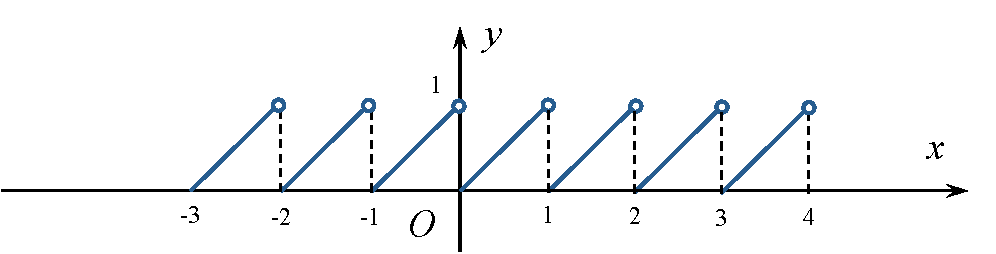
\includegraphics[width=0.7\textwidth]{./images/Ch01/f1.pdf}\\
	  	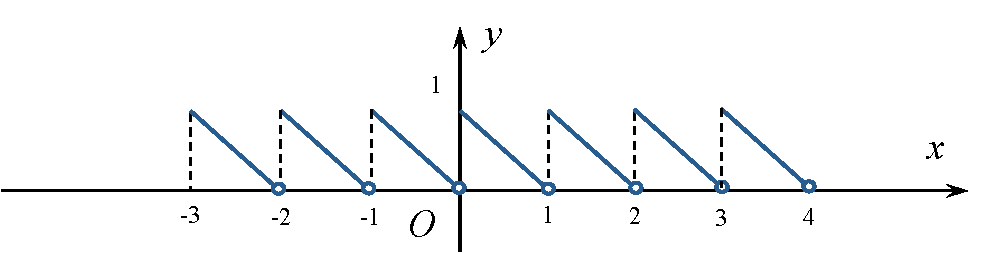
\includegraphics[width=0.7\textwidth]{./images/Ch01/f2.pdf}\\
	  	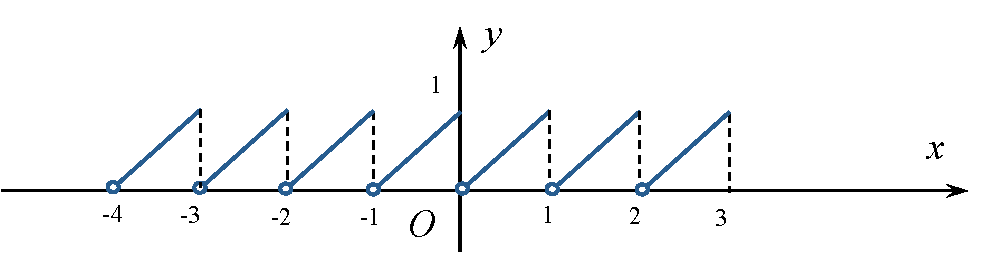
\includegraphics[width=0.7\textwidth]{./images/Ch01/f3.pdf}
	  \end{center}
	  \item 如左图,将单位圆上的点$Q$映射成数轴上的点$P$的映射称为{\it 球极投影映射},
	  请给出:
	  \begin{enumerate}[(1)]
	    \item $Q$的极角$\theta$与$P$的横坐标$x_P$的对应关系;
	    \item $Q$的坐标$(x_Q,y_Q)$与$P$的坐标$(x_P,y_P)$的对应关系;
	    \item 思考(选作):参考右图,给出将一个单位球面映射为二维平面的
	    {\it 三维球极投影映射},写出具体的对应关系。
	  \end{enumerate}
	\begin{center}
		\resizebox{!}{5cm}{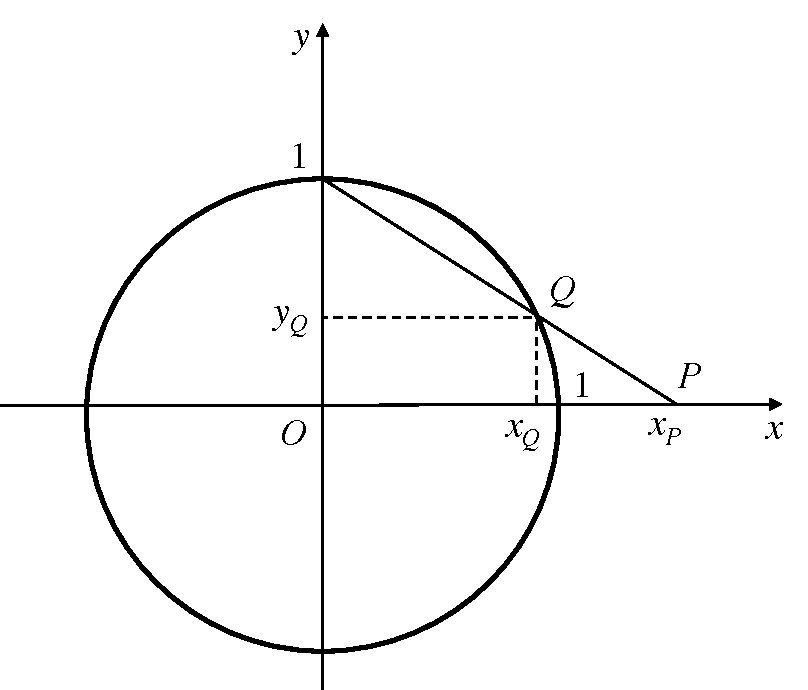
\includegraphics{./images/ch01/sphereline2D.pdf}}\quad
		\resizebox{!}{5cm}{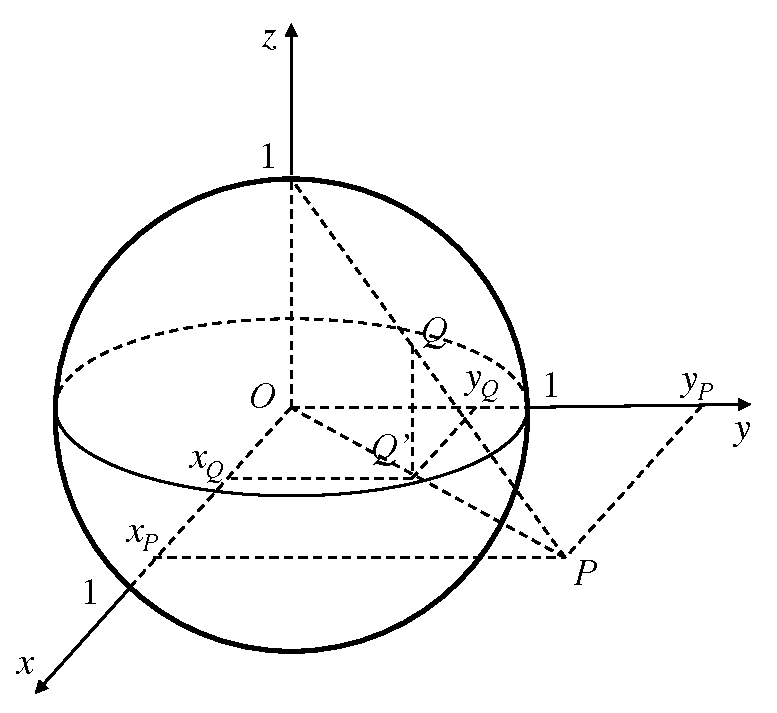
\includegraphics{./images/ch01/sphereline3D.pdf}}
		
		\it \small 第4题图
	\end{center}
%	\item (选作)对任意$x_0\in\mathbb{R}$,试给出两个数列$\{x^{(1)}_n\}$和
%	$\{x^{(2)}_n\}$,而且分别为有理数列和无理数列,且都以$x_0$为极限。
	\item (选作)以椭圆$\df{x^2}{a^2}+\df{y^2}{b^2}=1$的左焦点为极点,
	沿$x$轴正向取极轴,求该椭圆的极坐标方程。
	\end{enumerate}
\end{ext}

\newpage
\section{数列的极限}

极限概念的引入是微积分发展史上具有革命性的一步,
为奠定微积分理论“无可非议”的扎实
基础提供了可能。后续我们将要学习的导数、积分、
级数等重要概念都是以极限的形式定义的。

数列极限是极限问题中最为简单的一类,也是性质非常典型的一类,
可以作为我们后续学习函数极限的基础。

\bs
{\bf 数列}就是按一定规律排列的无穷多个(相同或不相同的)数,一般记作:
\pss{\baa 有序性是数列的重要特征,
改变了数列中数的排列顺序将得到不同的数列}
$$a_1,a_2,\ldots,a_n,\ldots\quad\mbox{或者}\quad\{a_n\}.$$

$\{a_n\}$的实质是定义在$\mathbb{Z}_+$上的函数,因此数列也被称为
{\it 整标函数}或{\it 整序函数}。如果在平面直角坐标系内作图,
可以将其视为一个动点随$n$增大所留下的离散的运动轨迹。

下面是一些数列的例子:
\begin{enumerate}[(1)]
  \setlength{\itemindent}{1cm}
  \item[(1)] $\left\{\df{n+1}n\right\}:\df 21,\df 32,\df43,\df54,\df65,\ldots$
  \item[(2)] $\left\{\df{(-1)^n}n\right\}:-1,\df12,-\df13,\df14,-\df15,\df16,\ldots$
  \item[(3)] $\{n^2\}:1,4,9,16,25,36,\ldots$
  \item[(4)] $\left\{n^{(-1)^n}\right\}:1,2,\df13,4,\df15,6,\ldots$
\end{enumerate}

\bs
{\bf 思考:}数列与集合有哪些区别?

\ifhint
提示:1、有序-无序;2、无限-可能有限;3、元素可重复-元素不可重复.
\fi

\subsection{数列的极限}

形象地说,数列$\{a_n\}$的{\it 极限},
\pss{微积分中的极限概念不同于现实生活里的极限,
现实中的极限是指可能达到的最大或最小值,类似于我们所说的
上确界和下确界。例如:人类速度的极限}
就是$a_n$的值随$n$的不断增大而趋向的某个{\it 确定}的值,
当然,对于不同的$\{a_n\}$,这个确定的值不一定都存在!例如:
\begin{enumerate}[(1)]
  \setlength{\itemindent}{1cm}
  \item $\left\{\df1n\right\}$
  的值随着$n$不断增大会越来越趋近于$0$,因此其极限为$0$;
  \item $\{n\}$的取值会越来越大,甚至可以超过任何事先给定给定的值,
  因此也不会趋于任何确定的值,极限不存在;
  \item $\{(-1)^n\}$的取值在$1$和$-1$上反复交替,从整体上看,
  既不能说它趋近与$1$,也不能说它趋近于$-1$,所以极限也不存在。
\end{enumerate}

在直观理解的基础上,我们主要关注这样一个问题:{\it 在数学上如何表达这种
趋向某个确定值的特征,或者说,如何给出数列极限的数学定义?}

以下的定义由数学家Weierstrass最终完成(注意,不是发明),
\pss{现行的极限符号$\lim$据说由数学家Hardy(1877-1947)引入,
而最初提出通过引入极限来解决微积分理论不严密问题的人是
法国数学家d'Alembert}
这是被数学界最广泛接受的一种极限定义:

\begin{thx}
	对于数列$\{a_n\}$,若存在常数$a$,对任意$\e>0$(不论它有多小),
	都存在$N\in\mathbb{Z}_+$,使对任意$n>N$,都有
	$$|a_n-a|<\e$$
	成立,则称{\bf 数列$\{a_n\}$存在极限(或收敛)},
	常数$a$称为该数列的极限,记为
	$$\lim_{n\to\infty}a_n=a\quad
	\mbox{或}\quad
	a_n\to a\;(n\to\infty)$$
	若上述常数$a$不存在,则称{\bf 数列$\{a_n\}$不存在极限}(或{\bf 发散})。
\end{thx}

从几何上看(如图\ref{fig:e-N-def}所示),数列$\{a_n\}$以$a$为极限,
意味着随着$n$的增大,$a_n$可以{\it 无限}地靠近$a$。
为了表达这种“无限靠近”,数学上可以这样来解释:
对于以$a$为中心的任意小的邻域$(a-\e,a+\e)$
(图上的蓝色阴影部分),只要把$n$取得{\it 充分大}($N$的意义就是为了界定这个所谓的充分大
\ps{显然,$\e$取得越小通常意味着$N$要取得越大,但必须注意的是$N$和$\e$
之间并不是简单的函数对应关系,因为如果某个$N$可以满足命题要求,
则$N$加任意的正常数显然也满足}
),则$a_n$都将落在$(a-\e,a+\e)$之内。
	
\begin{figure}[h]
	\centering
	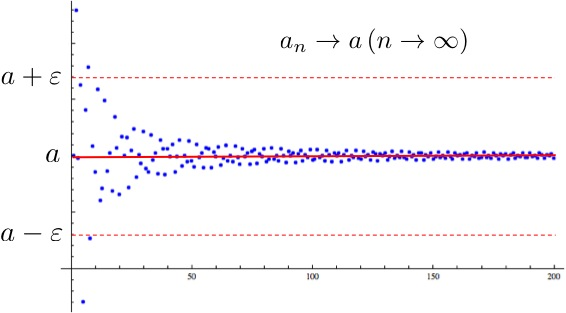
\includegraphics[width=0.45\textwidth]{./images/ch01/en1.jpg}\;
	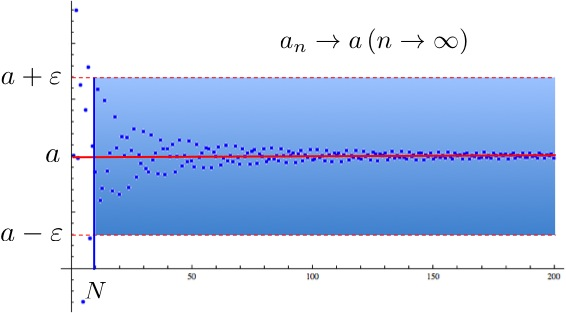
\includegraphics[width=0.45\textwidth]{./images/ch01/en2.jpg}\\
	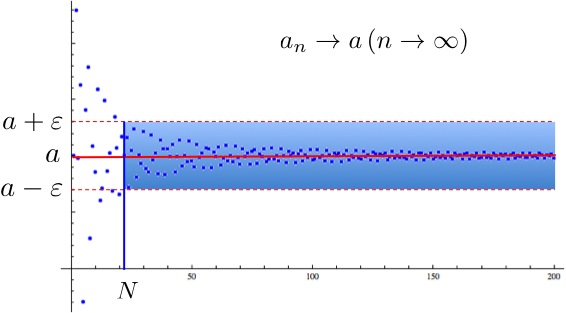
\includegraphics[width=0.45\textwidth]{./images/ch01/en3.jpg}\;
	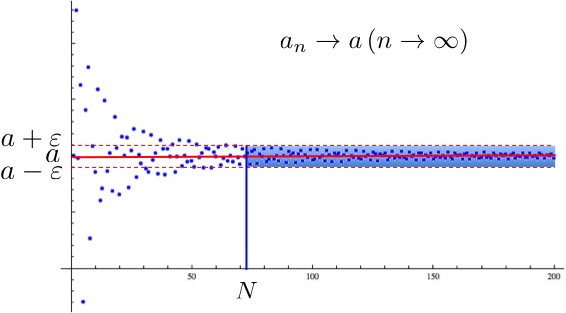
\includegraphics[width=0.45\textwidth]{./images/ch01/en4.jpg}
	\caption{不论$\e$取得多小,总存在对应的$N$,使得$n>N$对应的所有
	$a_n$都落在$U(a,\e)$之内}
	\label{fig:e-N-def}
\end{figure}

\begin{shaded}
	\pss{\centering
	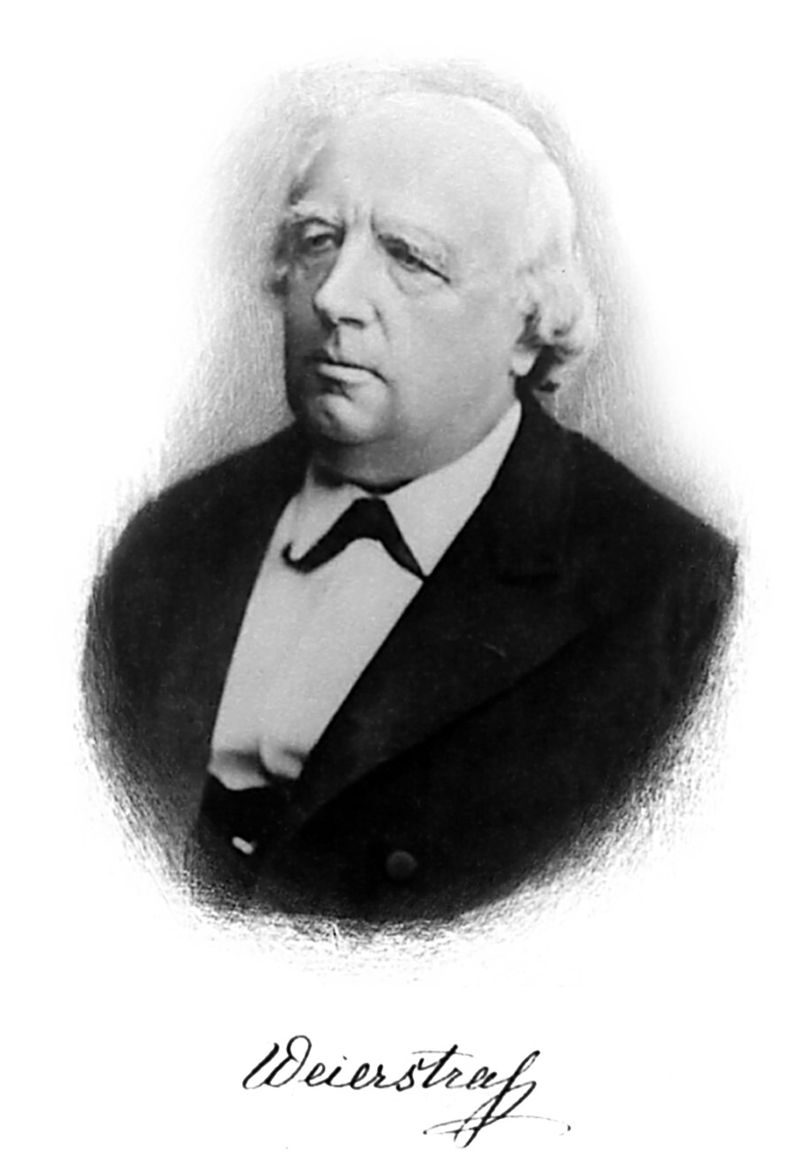
\includegraphics[width=0.7\marginparwidth]{./images/ch01/800px-Karl_Weierstrass.jpg}\\
	\href{https://en.wikipedia.org/wiki/Karl_Weierstrass}{K. Weierstrass(1815-1897)}\\
	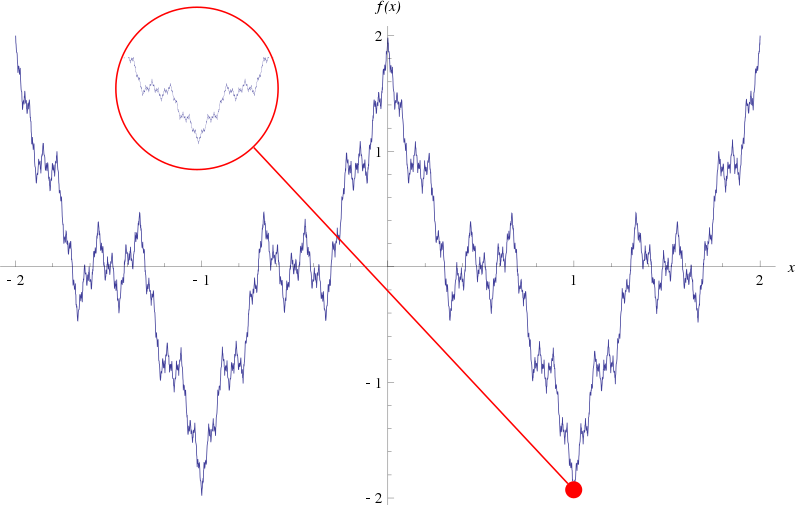
\includegraphics[width=0.7\marginparwidth]{./images/ch01/795px-WeierstrassFunction.svg.png}\\
	著名的\href{https://en.wikipedia.org/wiki/Weierstrass_function}{Weierstrass函数},处处连续,但处处不可微
	}

	关于极限的定义,历史上曾经有过很长时间的讨论,当时的许多数学家都尝试
	过给出一个“合适”的极限定义,例如:Cauchy是这样描述极限的:
	
	{\kaishu
		当属于一个变量的相继值无限地趋近某个固定值时,如果以这样一种方式告终,
		变量值同固定值之差小到我们希望当任意小,那么这个固定值就成为其他所有值的极限。
	}
	
	这个定义中所描述的“趋近”这个行动,很难说是一种令人满意的表达方式。趋近是指
	一种实际的动作吗?如果是,是否意味着我们在讨论极限时,必须把时间和空间的概念
	包含在内?此外,什么才是这个过程的“告终”?

	相对而言,Weierstrass的极限定义里,没有任何动作,不涉及任何时间,完全
	是一个“{\it 静态的而非动态的定义}”,同时又是一个“{\it 代数的而非几何的定义}”。
	定义的核心是一个关于不等式的断言(命题)。最重要的是,利用它能够很容易地
	证明各种关于极限的定理,例如“和的极限等于极限的和”、“极限的保号性”。
	至此,对于类似的定理终于可以像Euclid的几何命题一样完全地严格化了。
	这是微积分发展历史上一个巨大的进步。
	
	Weierstrass被称为“{\it 现代分析学之父}”,《微积分的历程》一书这样评价他:
	{\kaishu
		19世纪,数学家们将微积分的严格性提高到一个新的水平。然而,按照我们今天的标准,
		这些成就并不是无可挑剔的。当你拜读那个时期的数学文献时,犹如聆听音乐大师肖邦
		在一架三两琴键失调的钢琴上演奏乐章,固然能够怡然自得地鉴赏音乐的神韵,不过
		间或也会听到些许畸变之音。只有在微积分中消除不精确的最后痕迹,分析论证变成对于
		一切实用目的都是无可置疑的时候,数学的新纪元才能到来,Weierstrass正是
		实现这个最后转变的最大功臣。 
		
		\ldots\ldots
		
		Weierstrass学派通过Weierstrass本人或者他的门生们发表的研究成果,对分析学
		赋予逻辑上的一种无与伦比的精确性。他矫正了许多难以捉摸的错误概念,证明了大量
		重要的定理,并且构造出一个令数学家们惊叹不已的处处连续而又不可微的函数的反例。
	}
	
	Weierstrass同时还是一名出色的数学教育家,Hiene(1821-1881)和Cantor都是他的门生。
\end{shaded}
	
前述定义更为简洁的写法:
\ps{这种纯符号的表述方式固然简洁,但要正确掌握,
必须首先对更完整的文字表述有准确的理解,否则不建议随意使用}
$$\forall\e>0,\exists N\in\mathbb{Z}_+,\forall n>N,
|a_n-a|<\e.\eqno{(1)}$$

{\bf 讨论:}以下说法和$(1)$等价的是:
\begin{enumerate}
  \setlength{\itemindent}{1cm}
  \item[(2)] $\forall\e>0$,$\exists N$,$\forall
  n>N$,$|a_n-a|\leq\e.$ \hfill{$\surd$} 
  
  \ifhint\quad 提示:只要强调$n>N$为正整数即可,
  根据需要$N$总是可以取得更大,无所谓是不是正整数。\fi

  \item[(3)] $\exists N\in\mathbb{Z}_+$,$\forall\e>0$,$\forall
  n>N$,$|a_n-a|<\e.$ \hfill{$\times$}
  
  \ifhint\quad 提示:(3)可以推出(1),但反之不然。事实上,由(3)可以推出,
  $\{a_n\}$仅有有限项的值不等于$a$,但显然不是所有收敛的数列都有此
  性质,例如$\{1/n\}$\fi

  \item[(4)] $\forall\e>0$,仅有有限多个$n$,使得$|a_n-a|\geq\e.$
  \hfill{$\surd$}
  
  \ifhint\quad 提示:由(4),仅有有限多个$a_n$不满足$|a_n-a|<\e$,
  则我们总可以取其中下标最大的下标作为$N$,
  则当$n>N$时,总有$|a_n-a|<\e$,即(1)成立;反之,由
  (1),最多有不超过$N$个$a_n$不满足$|a_n-a|<\e$。
  故(4)与(1)等价。\fi
  
  \item[(5)] $\forall\e>0$,总有无穷多个$n$,使得$|a_n-a|<\e.$
  \hfill{$\times$} 
  
  \ifhint\quad 提示:考虑反例:$a_n=(-1)^n$,取$a=1$。\fi

  \item[(6)] $\forall\e>0$,要使$|a_n-a|<\e$,
  只须$n$充分大 \hfill{$\surd$}
  
  \ifhint\quad 提示:语序有变化,但逻辑关系和含义并未发生改变。\fi

  \item[(7)] $\forall\e>0,\exists N\in\mathbb{Z}_+,\forall
  n>N,|a_n-a|<2\e$\hfill{$\surd$}
  
  \ifhint\quad 提示:由于$\e$是任意的,$2\e$和$\e$的取值范围并没有区别,都是
  $(0,+\infty)$!事实上,在用定义证明极限时,完全可以使用$C\e$,
  其中$C\in\mathbb{R}$为给定的常数,这是数列极限最常用的一种等价定义。\fi
\end{enumerate}

\bs
\egz 证明:$\limn(-1)^n\df1{n^2}=0.$

分析:截止目前,我们还没有学习其他可以用来判定或证明极限
的结论,因此本题只能用定义证明。

用定义证明极限,就是要验证所给的数列$\left\{(-1)^n\df1{n^2}\right\}$
以及常数$0$能够满足极限定义中的命题。为此,我们不难发现,
对于任意给定的$\e$,找到与之对应的$N$是证明的关键。反之,
如果能够证明这样的$N$有时(对于某些$\e$)是找不到
(不存在)的,则可以说明该数列的极限不是题目中给定的常数。

为了找$N$,我们可以从命题的结论出发,即要使
$$\left|(-1)^n\df1{n^2}-0\right|<\e,$$
显然,该式等价于$n>1/{\sqrt{\e}}$。这就意味着,只要取$N$
为某个大于$1/\sqrt{\e}$的整数,则对所有的$n>N$,就都有
$n>1/\sqrt{\e}$,从而就有结论中的不等式成立了。

在取$N$的值时,我们通常会用到下取整函数,例如,可以取
$N=\left[1/\sqrt{\e}\right]+1$(注意
$\left[1/\sqrt{\e}\right]+1>1/\sqrt{\e}$)。

证:对任意$\e>0$,令$N=\left[1/\sqrt{\e}\right]+1$
\ps{直接给出与$\e$相关的$N$的值,是最直接的说明$N$的存在性的途径},
则对任意$n>N$,有
$$\left|(-1)^n\df1{n^2}-0\right|=\df1{n^2}<\df1{N^2}
<\df1{(\sqrt{\e})^2}=\e,$$
由极限的定义,即证。
\fin 

\bs
{\bf 课堂练习:}证明
$$\limn\left(\df n{n+1}\right)^2=1$$

\ifhint
提示:对任意$\e>0$,令$N=\left[2/\e\right]+1$,则对任意$n>N$,有
$$\left|\left(\df
n{n+1}\right)^2-1\right|=\df{2n+1}{(n+1)^2}<\df{2(n+1)}{(n+1)^2}
<\df2{n+1}<\df2n<\df2N<\e,$$
由极限的定义,即证。\fin
\fi

有些时候,$N$的值不一定能直接表示为与$\e$相关的形式,
但借助已知的极限,我们常常可以间接地给出$N$。

\bs
\egz 证明:若$\limn a_n=a$,则$\limn|a_n|=|a|$

证:对任意$\e>0$,由$\limn a_n=a$可知,存在$N_1\in\mathbb{Z}_+$,
对任意$n>N_1$,有
$$|a_n-a|<\e.$$
于是令$N=N_1$,\ps{利用$N_1$的存在性间接说明了$N$的存在性}
则对任意$n>N$,有
$$||a_n|-|a||\leq|a_n-a|<\e,$$
由极限的定义,即证。\fin 

\bs
{\bf 课堂练习:}证明:若$|q|<1$,则$\limn q^n=0$。

\ifhint
提示:令$N=\left[\log_{|q|}\e\right]+1$
\fi

\bs
{\bf 思考:}已知$|q|>1$时,$\{q^n\}$发散,请问该如何证明?

\ifhint 
提示:有两种可行的途径:一是利用极限定义的反面说法(或其反命题),
二是利用有界性(后面我们将证明收敛的数列必有界)。
\fi

\begin{shaded}
	{\bf 极限定义的反面说法}
	
	参照此前对反面说法的介绍,由数列$\{a_n\}$以$a$为极限的定义:
	$$\limn a_n= a\quad\Leftrightarrow\quad\forall\e_0>0,
	\exists N\in\mathbb{Z}_+,\forall n>N,|a_n-a|<\e_0,$$
	不难写出{\bf 数列$\{a_n\}$不以$a$为极限}的定义:
	$$\limn a_n\neq a\quad\Leftrightarrow\quad\exists\e_0>0,
	\forall N\in\mathbb{Z}_+,\exists n_0>N,|a_{n_0}-a|\geq\e_0.$$
	
	\bs
	下面用这个定义来证明几个例子:
	
	\egz 证明:$\limn\df 1n\neq 1$.
	
	证:取$\e=\df12$,对任意$N\in\mathbb{Z}_+$,令$n_0=\max\{3,N+1\}>N$,
	从而
	$$\left|\df1{n_0}-1\right|=1-\df1{n_0}\geq 1-\df13=\df23>\e,$$
	由极限的反面定义,即证。\fin
	
	\bs
	\egz 证明$\{(-1)^n\}$发散。
	\ps{证明数列$\{a_n\}$发散意味着要证明任意的$a$都不是其极限}
	
	证:任取$a\in\mathbb{R}$,只需证明$\limn(-1)^n\ne a$。以下不妨设$a>0$。
	
	取$\e=1$,对任意$N\in\mathbb{Z}_+$,令$n_0=\max\{2[N]+1,1\}>N$,则
	$$\left|(-1)^{n_0}-a\right|=|-1-a|=a+1>\e,$$
	由极限的反面定义,即证。\fin
	
	相对于使用的反证法,用反面定义证明极限不存在,形式上更简洁,但
	却不是特别直观和容易理解。因此很多时候会用反证法来证明这样的问题。
	
	\bs
	{\bf 思考:}数列发散可能有哪些不同的情形?

	\ifhint
	答:趋向无穷(例如:$\{n\}$),或
	反复振荡(例如:$\left\{(-1)^n\right\}$)。
	\fi
\end{shaded}

\subsection{数列极限的性质}

\pss{以下几个性质的证明,可以作为用极限定义证明命题的典型例子,
应重点理解、掌握。}

{\bf 1. 唯一性}
\begin{thx}
	{\bf 定理:}数列极限若存在,必唯一。
\end{thx}

下面的证明需要用到如下的命题:设$a,b\in\mathbb{R}$,若对任意$\e>0$,
有$|a-b|<\e$,当且仅当$a=b$。
\ps{也即:两个确定的数如果可以无限靠近(小于任意给定的距离),
则意味着它们相等。}

证:设$a,b$均为数列$\{a_n\}$的极限。

对任意$\e>0$,由$\limn a_n=a$,存在$N_1\in\mathbb{Z}_+$,
对任意$n>N_1$,有$|a_n-a|<\e$;

同理,由$\limn a_n=b$,存在$N_2\in\mathbb{Z}_+$,
对任意$n>N_2$,有$|a_n-b|<\e$。

令$N=\max\{N_1,N_2\}$,则当$n>N$时,有
$$|a-b|\leq|a_n-a|+|a_n-b|<2\e,$$
由$\e$的任意性可知,必有$a=b$,即证。\fin

\pss{“记录重大技术突破的技术发展史其实就是一部人类社会发展的技术选择史”。
可以说,是唯一性的要求决定了当前的极限定义。从这个意义上说,
目前使用的极限定义其实也是一种约定。}
\begin{figure}[h]
	\centering
	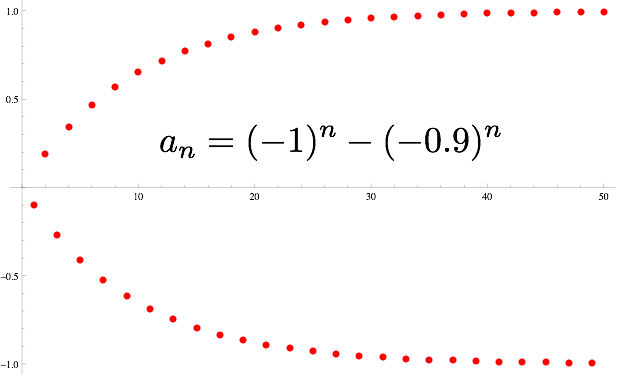
\includegraphics[width=0.5\textwidth]{./Images/Ch01/1-0.9n.jpg}
	\caption{一个不收敛的数列}
	\label{fig:an-diverse}
\end{figure}

\bs
{\bf 2. 有界性}
\begin{thx}
	{\bf 定理:}数列$\{a_n\}$若收敛,则{\it $\{a_n\}$有界},
	即:存在$M>0$,对任意$n\in\mathbb{Z}_+$,恒有$|a_n|\leq M$。	
\end{thx}

提示:利用$\e$的特定取值“控制”$n>N$的部分,而在$N$之前的
有限多个数构成的集合自然是有界的。

解:记$\limn a_n=a$。由极限的定义,对{\b$\e=1$},存在$N\in\mathbb{Z}_+$,
对任意$n>N$,有
$$|a_n-a|<\e=1\quad\Rightarrow\quad |a_n|<|a|+1.$$
记$M=\max\{|a|+1,|a_1|,|a_2|,\ldots,|a_{[N]+1}|\}$,则对
任意$n\in\mathbb{Z}_+$,均有
$$|a_n|\leq M,$$
即证。\fin

\begin{figure}[h]
	\centering
	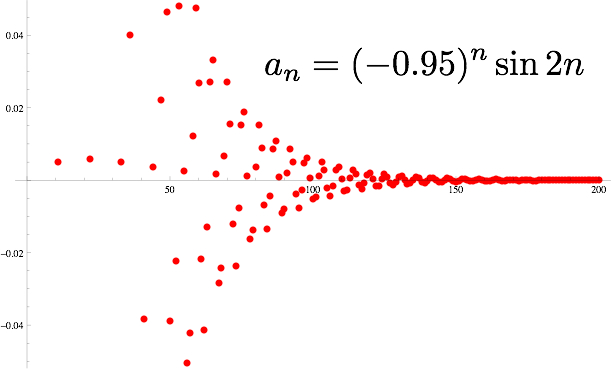
\includegraphics[width=0.5\textwidth]{./Images/Ch01/sin2nn.jpg}
	\caption{一个收敛的数列}
	\label{fig:an-converge}
\end{figure}

该性质的等价命题(逆否命题)常被用来证明数列发散:
{\bf 如果某数列无界,则必发散。}

\begin{shaded}
	\egz 讨论$\{\sqrt[n]{n!}\}$的敛散性。
	\pss{\centering
	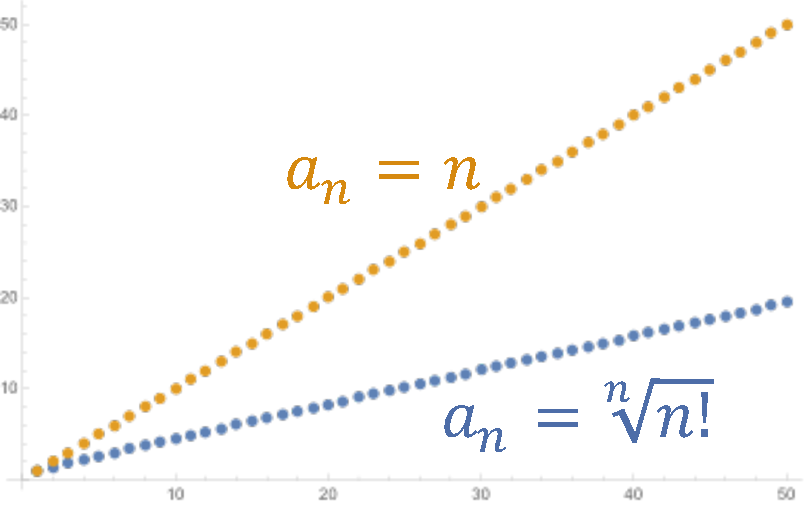
\includegraphics[width=0.9\marginparwidth]{./Images/Ch01/nnnf.pdf}}

	提示:对任意$M>0$,当$n$充分大时,总有$n!>M^n$,
	故$\{\sqrt[n]{n!}\}$无界,从而发散。

	证:对任意$M>0$,令$N=[2M]+1$,则当$n>N$时,总有$n>2M$。此时
	$$\df{n!}{M^n}=\df{N!}{M^N}\cdot\df{N+1}{M}
	\cdot\df{N+2}{M}\ldots\df{n}{M}>\df{N!}{M^N}\cdot2^{n-N+1}.$$
	注意到$\df{N!}{M^N}$为有限值,而$2^{n-N+1}$随着$n$的增大趋于正无穷,
	故当$n$充分大时,必有
	$$\df{n!}{M^n}=\df{N!}{M^N}\cdot2^{n-N+1}>1,$$
	从而$\sqrt[n]{n!}>M$,也即$\{\sqrt[n]{n!}\}$无界,故发散。\fin
\end{shaded}

\bs
{3. 保号性}
\begin{thx}
	{\bf 定理:}设$\lim\limits_{n\to\infty}a_n=a>0$,则存在$N$,
	对任意$n>N$,$a_n>0$	
\end{thx}

证:由$\lim\limits_{n\to\infty}a_n=a>0$,对$\e=a/2$,存在
$N$,对任意$n>N$,
$$|a_n-a|<\e=a/2\quad\Rightarrow\quad \df32a>a_n>a/2>0,$$
即证。\fin
		
保号性有几种不同的表达形式:
\begin{thx}
	\begin{enumerate}[\bf 推论1:]
% 	  \setlength{\itemindent}{1cm}
	  \item 对任意$n\in\mathbb{N}$,$a_n\geq
	  0$, $\lim\limits_{n\to\infty}a_n=a$, 则$a\geq 0$
	  \item 设$\lim\limits_{n\to\infty}a_n=a\ne
	  0$, 则$\exists N$,当$n>N$时,$|a_n|>|a|/2$
	  \item  设$\lim\limits_{n\to\infty}a_n=a$, 且最多有有限
	  个$a_n$小于零, 则$a\geq 0$
	\end{enumerate}	
\end{thx}

保号性的实质,是{\it 极限运算保持不等号的方向
\ps{但严格大(小)于可能变成大(小)于等于}不变},
若已知$\limn a_n=a,\limn b_n=b$,则
$$a_n\geq b_n\,(n\in\mathbb{Z}_+)\quad\Rightarrow
\quad\limn a_n\geq\limn b_n.$$

\bs
{\bf 4. 数列与子数列的敛散性的关系}

{\bf 子数列}是指从原数列中“取出”无穷多个数所构成的新数列,
新数列中每个数出现的先后次序与原数列中相一致。子数列通常记为
$\{a_{n_k}\}$,其中$\{n_k\}$必须是一个严格单调递增的正整数列。
显然,对任意$k\in\mathbb{Z}_+$,$n_k\geq k$。

例如,数列$\{a_n\}$的{\it 奇子列}和{\it 偶子列}可分别
记为$\{a_{2k}\}$、$\{a_{2k-1}\}$,有时也直接写为
$\{a_{2n}\}$、$\{a_{2n-1}\}$。

在子数列中,$k$是真正的自变量,$n_k$是随$k$变化的,或者说,
如果将子数列看成是两个整序函数的复合函数,
则$n_k$可以视为该复合函数的一个中间变量。因此,相应地,其
极限的定义如下:

{\bf 子数列$\{a_{n_k}\}$以$a$为极限},
是指:对任意$\e>0$,存在$K\in\mathbb{Z}_+$,使对任意$k>K$,总有
$$|a_{n_l}-a|<\e.$$
记为
$$\lim\limits_{k\to\infty}a_{n_k}=a,\quad 
\mbox{或}\quad a_{n_k}\to a\;{(k\to\infty)}.$$

\begin{thx}
	{\bf 定理(收敛数列与其子数列的关系):}数列$\{a_n\}$收敛,
	当且仅当它的所有子列均收敛到相同的极限。
\end{thx}

证:充分性是显然的,因为$\{a_n\}$可以看成是自身的一个子列。

下面证明必要性。设$\limn a_n=a$,则对任意$\e>0$,存在$N\in\mathbb{Z}_+$,
使对任意$n>N$,有$|a_n-a|<\e$。

设$\{a_{n_k}\}$为$\{a_n\}$的任一子列。令$K=N$,则由$\{n_k\}$严格单调递增,
可知对任意$k>K$,都有$n_k>n_K\geq K=N$,从而 
$$|a_{n_k}-a|<\e.$$
也即$\lim\limits_{k\to\infty}a_{n_k}=a$。因为$\{a_{n_k}\}$是任意的,即证。
\fin

\bs
该定理的一个明显用途,是判定一些数列的发散。也即,{\bf 若某个数列存在
发散的子数列,或者存在两个收敛到不同极限的子数列,则该数列必发散。}

\egz 证明数列$\{(-1)^n\}$发散。

证:取该数列的偶子列和奇子列,分别即为$\{a_{2k}\}$和$\{a_{2k-1}\}$。显然,
对任意$k\in\mathbb{Z}_+$,都有
$$a_{2k}\equiv 1,\quad a_{2k-1}\equiv -1,$$
因此
$$\lim\limits_{k\to\infty}a_{2k}=1,\quad
\lim\limits_{k\to\infty}a_{2k-1}=-1.$$
由二者极限不相等可知原级数发散,即证。\fin

这种方法证明发散,比前面使用数列收敛的反面定义或反证法
来证明要更加简洁,也更加直观。

\bs
\egz \ps{KD教材2.2.2节-例4}
证明数列$\left\{n^{(-1)^n}\right\}$发散。

提示:原数列存在发散子列$\left\{(2n)^{(-1)^{2n}}\right\}=\{2n\}$。

\bs
{\bf 思考:} 证明$\left\{\left(1+\df1{\sqrt n}\right)
\sin\df{\pi\sqrt n}2\right\}$
发散。

\ifhint
提示:取$n_k=k^2$。 
\fi

\begin{shaded}
	证明数列发散往往比证明其收敛更困难,因为要证明所有的数都不是其极限。
	因此,在证明方法上,也更加多样。下面的例子请自行阅读,我们不作要求。

	\egz 证明:$\{\sin n\}$发散。

	\pss{\centering
	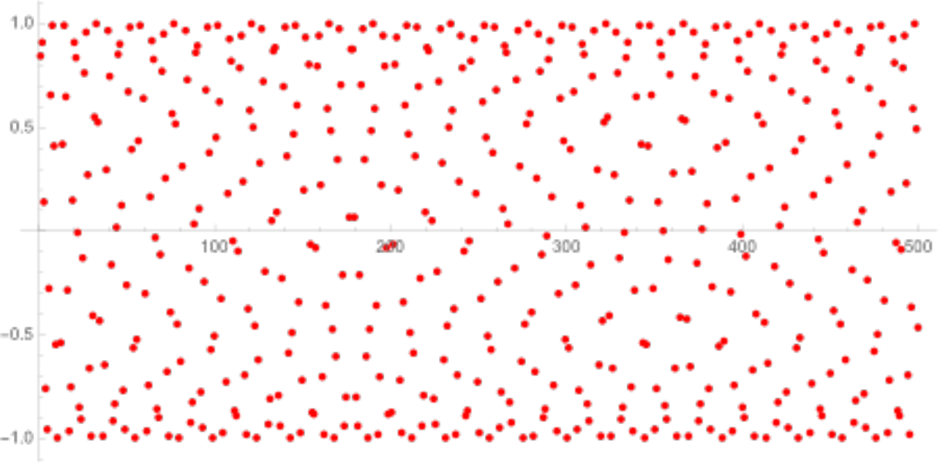
\includegraphics[width=0.9\marginparwidth]
	{./images/ch01/sin-n.pdf}\\
	数列$\{\sin n\}$
	}
	
	证法一:反证法。设有$\limn\sin n=a$,则
	$$\limn[\sin(n+2)-\sin n]=0.$$
	进而由
	$$\sin(n+2)-\sin n=2\sin 1\cos(n+1),$$
	可得$\limn\cos(n+1)=0$。又
	$$\cos(n+1)=\cos n\cos 1-\sin n\sin 1,$$
	可得$\limn\sin n=0$。如此就有
	$$\limn\sin n=\limn\cos n=0,$$
	显然与$\sin^2n+\cos^2n=1$矛盾。\fin
	
	证法二:注意到当$x\in[2k\pi+\pi/4,2k\pi+3\pi/4]\,
	(k\in\mathbb{N})$时,总有
	$$\sin x>\sqrt2/2.$$
	由于此类区间的长度均超过$1$,故其中必包含至少一个自然数。
	于是对每个$k\in\mathbb{N}$,
	可取自然数$n^{(1)}_k\in[2k\pi+\pi/4,2k\pi+3\pi/4]$,
	显然$\{\sin{n^{(1)}_k}\}$构成了$\{\sin
	n\}$的一个子列。
	
	若$\{\sin n\}$收敛,则$\{\sin{n^{(1)}_k}\}$也收敛,且与之极限相同。由极限的保号性,
	可知$\{\sin{n^{(1)}_k}\}$的极限不小于$\sqrt2/2$,从而$\{\sin
	n\}$的极限应大于等于$\sqrt2/2$。
	
	同理,利用区间$[2k\pi+5\pi/4,2k\pi+7\pi/4]\,(k\in\mathbb{N})$,
	可构造$\{\sin n\}$的另一个子列 
	$\{\sin{n^{(2)}_k}\}$。若$\{\sin n\}$收敛,同样利用保号性可证明其极限应小于等于$-\sqrt2/2$。
	
	以上两方面的结论矛盾,故假设错误,即证。\fin
\end{shaded}

该性质类似的一个结论如下:
\begin{thx}
	{\bf 拉链定理}:若某个数列的奇子列和偶子列收敛到相同的极限,
	则该数列收敛。
\end{thx}

请自行尝试证明该定理。注意,这个定理并不是子数列性质的简单推论。
此外,还请想一想,这个定理可以进一步推广吗?

事实上,拉链定理有更一般形式的推广:如果选择的多个子列按顺序
合并起来能够完全覆盖原数列,
或最多不能覆盖原数列中有限多个数,且这些子列均收敛于相同的极限,
则原数列收敛。
例如:{\it 若子数列$\{a_{3n}\},\{a_{3n-1},\{a_{3n-2}\}\}$
都收敛于$a$,
则$\{a_{n}\}$收敛于$a$。}

\begin{shaded}
{\bf Cauchy命题}

以下结论不容易证明,但结论很直观,了解即可:
\begin{tcolorbox}
	{\bf Cauchy命题}:若$\limn a_n=a$,
	则$\limn\df{a_1+a_2+\ldots+a_n}n=a$。\ps{证明参见菲赫金哥尔茨《微积分学教程》第一卷第一章第2节}
\end{tcolorbox}

这个结论也称为Cauchy{\it 极限},有着非常重要的应用,例如,今后我们会学习
下面的极限$\limn\sqrt[n]a=1,\,(a>0)$,于是立即可以得到
$$\limn\df1n(a+\sqrt[2]a+\sqrt[3]a+\ldots+\sqrt[n]a)=1.$$

\bs
此外,我们今后还会学习到极限运算和初等函数运算可以交换次序,
进而可以证明如下的定理:

\begin{tcolorbox}
	{\bf 定理:}设$a_n$均大于零,且$\limn\df{a_{n+1}}{a_n}=q$,则
	$\limn\sqrt[n]{a_n}=q$。	
\end{tcolorbox}

证:记$b_1=a_1$,$b_n=\df{a_n}{a_{n-1}}\;(n>1)$,则
$$a_n=b_n\cdot b_{n-1}\cdots b_1,$$
进而
$$\ln a_n=\ln b_n+\ln b_{n-1}+\ldots+\ln b_1,$$
已知$\limn b_n=q$,根据初等函数的性质,可得$\limn\ln b_n=\ln q$,
于是由Cauchy极限,
$$\limn\ln \sqrt[n]{a_n}=\limn\df1n\ln a_n=\limn\df1n\left(
\ln b_n+\ln b_{n-1}+\ldots+\ln b_1\right)=\ln q,$$
进而可得$\limn\sqrt[n]{a_n}=q$。\fin 

\bs
有了这个定理,我们很容易得到下面的结论:
\begin{tcolorbox}
	{\bf 定理:}设$a_n$均大于零,且$\limn a_n=a$,则
	$\limn\sqrt[n]{a_1a_2\ldots a_n}=a.$
\end{tcolorbox}
\end{shaded}

\begin{ext}
	{\centering\bf 习题1-2}
	
	\begin{enumerate}  
	  \item 用定义证明如下极限:
	  \begin{enumerate}[(1)]
	    \item $\limn\df{\sqrt{n^2+a^2}}n=1$;
	    \item $\limn0.\underbrace{999\ldots9}_{n\mbox{\footnotesize 个}}=1$;
	    \item $\limn(\sqrt[3]{n+1}-\sqrt[3]n)=0$;
	    \item $\limn\df{n^2-n-1}{2n^2+2n-4}=\df12$。
	  \end{enumerate}
	  \item 设数列$\{a_n\}$有界,$\limn b_n=0$,证明:$\limn a_nb_n=0$。
	  \item 设$\limn a_n=a\ne 0$,证明:存在$N\in\mathbb{Z}^+$,对任意
	  $n>N$,有$|a_n|>|a|/2$。
	\end{enumerate}
\end{ext}

\newpage
\section{函数的极限}

\subsection{函数极限的定义}

函数极限是我们后续定义导数、积分的概念的基础。从形式上看,
可以将它视为数列极限的推广,
但从直观意义上看,二者存在很大的不同。

不同于数列极限中自变量$n$只有趋于$\infty$(事实上是趋于$+\infty$)
一种趋势,函数中的变量$x$可能的变化趋势有六种,通常分为两大类:
\begin{itemize}
  \setlength{\itemindent}{1cm}
  \item {\it 自变量$x$趋于无穷}
  \pss{$x\to x_0^+$表示从$x$从大于$x_0$的部分趋近$x_0$,
  一般也称为从正向趋于$x_0$;类似地,$x\to x_0^-$称为从负向趋于
  $x_0$}
  $$x\to\infty,\quad x\to+\infty,\quad x\to-\infty$$
  \item {\it 自变量趋于$x$有限值$x_0$}
  $$x\to x_0,\quad x\to x_0^+,\quad x\to x_0^-$$
\end{itemize}

\bs
{\bf 思考:} $\limn f(n)=A\Leftrightarrow\limx{+\infty}f(x)=A$成立吗?

\ifhint
答:显然,$\limx{+\infty}f(x)=A$可以推出$\limn f(n)=A$,但反之不然,
\ps{事实上,$f(n)$的值域是$f(x)$值域的子集}

例如:$y=\sin\pi x$当$x\to+\infty$时不收敛,但$\limn\sin n\pi=0$。
\fi

\bs
{\bf 1.\;$x$趋于无穷时的函数极限}

参考数列极限的定义,我们可以给出函数当$x$趋于无穷时的极限的定义,这里
我们使用了较简略的写法:
\begin{thx}
	\begin{enumerate}%[(1)]
	  \item $\limx{+\infty}f(x)=A\quad\Leftrightarrow\quad
	  \forall \e>0,\exists X>0,\forall x>X,|f(x)-A|<\e$
	  \item $\limx{-\infty}f(x)=A\quad\Leftrightarrow\quad
	  \forall \e>0,\exists X<0,\forall x<X,|f(x)-A|<\e$
	  \item $\limx{\infty}f(x)=A\quad\Leftrightarrow\quad
	  \forall \e>0,\exists X>0,\forall |x|>X,|f(x)-A|<\e$
	  \ps{$x\to\infty$表示同时趋向正负无穷,其实质是远离任何一个
  	  固定的点,只有当趋于正负无穷的极限相同时该极限才有意义}
	\end{enumerate}
\end{thx}

显然,这三个极限定义的不同之处主要体现在如何表示$x$的范围方面。例如:
若考虑$x\to+\infty$时的极限,则要说明当$x$充分大(充分靠近$+\infty$)
时,可以使$|f(x)-A|<\e$成立。这里的充分大就可以表示为“{\it 存在
$X$,对任意的$x>X$}”。类似地,,若考虑$x\to\infty$时的极限,则要说明
当$x$充分靠近$\pm\infty$时,可以使$|f(x)-A|<\e$成立。而所谓的
“{\kaishu 充分靠近$\pm\infty$}”{\kaishu 也即"$|x|$充分大}",
因此可以表示为"存在$X$,对任意$|x|>X$"。

\bs
直观上看,若函数当$x$趋于无穷时的极限存在,则意味着其图像存在
{\bf 水平渐近线},例如:反正切函数(参见图\ref{subfig:arctan})
满足
\begin{itemize}
	\item $\limx{+\infty}\arctan x=\frac{\pi}{2}$,故
	当$x\to+\infty$时,$y=\arctan x$有水平渐近线$y=\frac{\pi}{2}$;
	\item $\limx{-\infty}\arctan x=-\frac{\pi}{2}$,故
	当$x\to-\infty$时,$y=\arctan x$有水平渐近线$y=-\frac{\pi}{2}$;
	\item 因为$\limx{+\infty}\arctan x\ne\limx{-\infty}\arctan x$,
	故极限$\limx{\infty}\arctan x$不存在。
\end{itemize}

\begin{figure}[h]
	\centering
	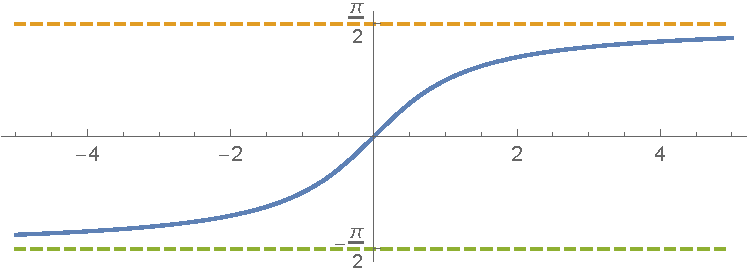
\includegraphics[width=0.5\textwidth]{./Images/Ch01/arcTanAsy.pdf}
	\caption{$\arctan x$和它的两条水平渐近线}
	\label{fig:arctanAsy}
\end{figure}
	
\bs

\egz 证明$\limx{+\infty}\df1{\sqrt x}=0$.

证:对任意$\e>0$,取$X=\df1{\e^2}$,则对任意的$x>X$,都有
$$\left|\df1{\sqrt x}-0\right|=\df1{\sqrt x}<\df1{1/\e}=\e,$$
由函数极限的定义,即证。\fin

\bs

{\bf 2.\;$x$趋于有限值时的函数极限}

\begin{thx}
	\begin{enumerate}%[(1)]
	  \item $\limx{x_0}f(x)=A\quad\Leftrightarrow\quad
	  \forall \e>0,\exists\delta>0,\forall
	  x\in U_0(x_0,\delta),|f(x)-A|<\e.$
	  \item $\limx{x_0^+}f(x)=A\quad\Leftrightarrow\quad
	  \forall \e>0,\exists\delta>0,\forall x\in
	  U_0^+(x_0,\delta),|f(x)-A|<\e.$
	  \pss{$U_0^+(x_0,\delta)=(x_0,x_0+\delta)$,也即$x_0$
	  的右半$\delta$邻域;同理,$U_0^-(x_0,\delta)$表示
	  $x_0$的左半$\delta$邻域}
	  \item $\limx{x_0^-}f(x)=A\quad\Leftrightarrow\quad
	  \forall \e>0,\exists\delta>0,\forall
	  x\in U_0^-(x_0,\delta),|f(x)-A|<\e.$
	\end{enumerate}
\end{thx}

无论是$x$趋于无穷时的极限还是$x$趋于有限值时的极限,定义的逻辑结构都是
一致的,唯一的不同就在于对$x$变化趋势的表述方法(有限领域和无穷领域的差别)。
抽象地说,以上的六个极限定义都是陈述了如下一个事实:{\kaishu 
$\limx{\Delta}f(x)=A$,也即:随着$x$越来越靠近$\Delta$
($\Delta$代表$x_0,x_0^+,x_0^-,\infty,+\infty$,$-\infty$之一),
$f(x)$的值越来越靠近$A$};或者说,{\it 要使$f(x)$充分
靠近$A$,只需$x$充分靠近$\Delta$}。这与我们对数列极限的定义是完全一致的。

\bs

{\bf 课堂练习:} \ps{KD教材习题3.1-1}
根据图形(图\ref{fig:limxexist})判断极限的存在性,若存在给出其值
\begin{figure}[h]
	\centering
	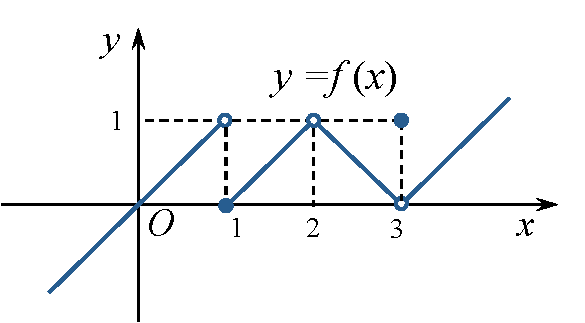
\includegraphics[width=0.4\textwidth]{./Images/Ch01/limxf.pdf}
	\caption{$\limx{1}f(x)$\underline{不存在}
	\quad $\limx{2}f(x)$\underline{$=1$}
	\quad $\limx{1}f(x)$\underline{$=0$}}
	\label{fig:limxexist}
\end{figure}

\bs
{\bf 讨论:}
\begin{enumerate}
  \setlength{\itemindent}{1cm}
  \item 为什么在定义中要求$0<|x-x_0|<\delta$,而不是$|x-x_0|<\delta$?
   
   \quad 答:因为极限表示的$x\to x_0$时的过程中函数值的变化趋势,
   与函数在$x_0$处的取值无关!例如:令$f(x)=|\mathrm{sgn}(x)|$,
   则$\limx{0}f(x)=1$,但是$f(0)=0$。
  \item 符号$f(x_0+0),f(x_0-0)$与$f(x_0)$是何关系?
  
  \quad 答:前两者分别表示左、右极限
  \ps{类似地,$x$趋向无穷时的极限也可以记为:$f(\infty)$,$f(+\infty)$
  和$f(-\infty)$}
  ,最后一个是函数值,三者相互无关。
  例如:令$f(x)=\mathrm{sgn}(x)$,则$f(x_0+0)=1$,$f(x_0-0)=-1$,
  $f(0)=0$。
\end{enumerate}

\bs
\egz 证明:$\limx{x_0}\sin x=\sin x_0$。

证:对任意$\e>0$,令$\delta=\e$
\ps{寻找合适的$\delta$是证明的关键},则当$0<|x-x_0|<\delta$时,有
$$|\sin x-\sin x_0|=2\left|\cos\df{x+x_0}2\right|
\left|\sin\df{x-x_0}2\right|\leq|x-x_0|<\delta=\e,$$
由函数极限定义,即证。\fin

\bs

\egz 证明:$\limx{1}x^2=1$。

证:对任意$\e>0$,令$\delta=\min\left\{\df12,\e\right\}$,
\ps{令$\delta\leq\df12$,作用在于使得$|x+1|$有界}
则当$0<|x-1|<\delta$时,有
$$|x^2-1|=|(x+1)(x-1)|<\df32\cdot\delta<\df32\e,$$
由函数极限定义,即证。\fin

注:和数列极限类似,在函数极限的定义中,最后不等式右端
的$\e$可以改写为$C\e$,
其中$C>0$为常数,所得命题与原定义等价。

\bs

\egz 设$\limx{x_0}f(x)=A$,用定义证明:$\limx{x_0}[f(x)]^3=A^3$

证:对任意$\e>0$,由$\limx{x_0}f(x)=A$,存在$\delta>0$,对任意
$0<|x-x_0|<\delta$,有
$$|f(x)-A|<\e.$$
不妨设$\e<1$,由上式可知$0<|x-x_0|<\delta$时,有$|f(x)|<|A|+1$。

综上,记$C=(|A|+1)^2+(|A|+1)|A|+A^2$,则当$0<|x-x_0|<\delta$时,总有
\begin{align}
	|f^3(x)-A^3|&=|f(x)-A||f^2(x)+f(x)A+A^2|\notag\\
	&\leq |f(x)-A|[|f^2(x)|+|f(x)||A|+A^2]\notag\\
	&<\e[(|A|+1)^2+(|A|+1)|A|+A^2]=C\e\notag,
\end{align}
有极限的定义,即证。\fin

\begin{shaded}
	\begin{tcolorbox}
		{\bf 函数极限的反面说法}
		\begin{itemize}
		  \item {\it $\limx{x_0}f(x)\ne A$}$\Leftrightarrow$ 
		    $\exists\e_0>0,\forall\delta>0, \exists x^*\in
		    U_0(x_0,\delta),|f(x^*)-A|\geq\e_0$ 
		  \item {\it $\limx{x_0}f(x)\ne A$不存在}$\Leftrightarrow$
			$\forall A\in\mathbb{R},\exists\e_0>0,\forall\delta>0, \exists x^*\in
		    U_0(x_0,\delta),|f(x^*)-A|\geq\e_0$ 
		\end{itemize}
	\end{tcolorbox}

	\egz 证明:Dirichlet函数在任意点处无极限。
	
	证:任取$x_0,A\in\mathbb{R}$,不妨设$A\ne 0$($A\ne 1$的情况同理可证)。
	
	令$\e_0=\df{|A|}2$,对任意$\delta>0$,由有理数的稠密性,总可以在
	$U_0(x_0,\delta)$内取得某个有理数$x^*$,从而$D(x^*)=0$,于是
	$$|D(x^*)-A|=|A|>\e_0,$$
	由上述的定义,可知当$x\to x_0$时$D(x)$无极限,又由$x_0$的任意性,可知
	$D(x)$处处无极限。\fin

	\bs
	
	{\bf 思考题:}证明:函数$f(x)=xD(x)$只在$x=0$处收敛。

	注意,证明应该包括两个部分,一是证明$xD(x)$在$x=0$处收敛,二是证明
	$xD(x)$在任意$x\ne 0$处发散。
\end{shaded}

\subsection{函数极限的基本性质}

参考数列极限的性质,可以类似地证明函数极限的下列性质。

\begin{thx}
	{\bf 唯一性:}函数极限若存在,必唯一。
	
	{\bf 有界性:}
	\begin{enumerate}[(1)]
	  \setlength{\itemindent}{1cm}
	  \item 若$\limx{+\infty}f(x)=A$,则$f(x)$当$x$充分大时有界
 	  \ps{\vspace{-2em}当$x$充分大时,也即:存在$X$,当$x>X$时}
	  \item 若$\limx{x_0}f(x)=A$,则$f(x)$当$x$充分靠近$x_0$时有界
 	  \ps{当$x$充分靠近$x_0$时,也即:存在$\delta>0$,
 	  当$x\in U_0(x_0,\delta)$时}
	\end{enumerate}
	{\bf 保号性:}
	\begin{enumerate}[(1)]
 	  \setlength{\itemindent}{1cm}
	  \item 若$\limx{+\infty}f(x)=A>0$,则当$x$充分大时,$f(x)>0$
	  \item 若$\limx{x_0}f(x)=A>0$,则当$x$充分靠近时$x_0$时,$f(x)>0$
	\end{enumerate}
\end{thx}

函数极限有界性和数列极限有界性的叙述存在的差异:
数列收敛则数列整体有界(数列极限中的数列整体都有界,
是由数列自身的“稀疏”特性所决定的),
函数收敛只能说明在趋近的过程中(或者充分靠近目标时)有界!

例如:极限$\limx{+\infty}\df1x=0$,但$\df1x$在定义域上无界;
类似地,$\limx{1}x=1$,但$x$显然也是无界的。

\bs
\begin{thx}
	{\bf 函数极限与数列极限的关系}({\kaishu Henie定理}):
	\pss{Henie(1821-1881),德国数学大师Weierstrass的学生。
	1872年证明:有界闭区间上的连续函数必是一致连续的。
	也即,如果把函数的定义限定在闭区间上,
	连续和一致连续的差别将随之消失。} 
	已知$\limx{x_0}f(x)=A$,若若数列$\{x_n\}$取值在$f(x)$的定义域内,
	且满足:$x_n\to x_0(n\to$ $\infty)$,$x_n\ne 0\;
	(n\in\mathbb{Z}_+)$,
	则必有$\limn f(x_n)=A$。
\end{thx}

证:已知$\limx{x_0}f(x)=A$,故对任意$\e>0$,存在$\delta>0$,
使对任意$x\in U_0(x_0,\delta)$,都有$|f(x)-A|<\e$。

设$\limn x_n=x_0$,则以上的$\delta>0$,存在$N\in\mathbb{Z}_+$,
使对任意$n>N$,都有$|x_n-x_0|<\delta$。从而,当$n>N$时,必有
$$|f(x_n)-A|<\e.$$
即证。\fin

对于$x\to x_0^+$和$x\to x_0^-$的情形,该定理显然也成立。

与上一节子数列有关收敛性质的用途一样,
\pss{由于计算函数极限有类似L'Hospital法则和Taylor公式
这样的工具,相对来说比计算数列极限方法更多样}
Henie定理的用途更多地是证明函数极限不存在。
当然,有时遇到一些不方便计算的数列极限,
也可能将其转化为对应的函数极限来计算。

\bs
\egz 证明:$f(x)=\sin\df 1x$当$x\to 0$时无极限。

证:令
$$x^{(1)}_n=\df1{n\pi},\quad
x^{(2)}_n=\df1{2n\pi+\frac{\pi}2},\quad n\in\mathbb{Z}_+$$ 
显然,$\limn x^{(1)}_n=\limn x^{(2)}_n=0$,且
$$f(x^{(1)}_n)\equiv0,\quad f(x^{(2)}_n)\equiv1,$$
进而
$$\limn f(x^{(1)}_n)=0\ne1=\limn f(x^{(2)}_n),$$
由Henie定理,即知极限不存在。\fin
	
\begin{figure}[h]
	\centering
	\includegraphics[width=0.5\textwidth]{./Images/Ch01/sin1x.pdf}
	\caption{以上所取的$x^{(1)}_n$和$x^{(2)}_n$分别取自图上绿色和黄色水平线与
	函数$\sin\df1x$的交点,事实上,对于任意的$a\in[-1,1]$(红色水平线),
	都可以取得类似的点列,用于构造证明所需的收敛到不同值得函数值数列,请思考以下如何写
	出其表达式?}
	\label{fig:sin1x1-1}
\end{figure}

提示:如图\ref{fig:sin1xa}

\begin{figure}[htbp]
	\centering
	\includegraphics[width=\textwidth]{./Images/Ch01/sin1xa.pdf}
	\caption{$x^{(a)}_n=\df1{2n\pi+\arcsin a},\quad n\in\mathbb{Z}_+$}
	\label{fig:sin1xa}
\end{figure}

\egz 用Henie定理证明Dirichlet函数在任意点处无极限。
	
证:
对任意$x_0$,定义
$$x_n=[x_0]+x_0\mbox{\it 小数部分的前}n\mbox{\it 位},$$
$$x_n^{(1)}=x_n+\df1n,\quad
x_n^{(2)}=x_n+\df{\sqrt2}n,$$
显然$\{x_n^{(1)}\}$和$\{x_n^{(2)}\}$分别为趋于$x_0$的有理和无理数列,而
$$\limn D(x_n^{(1)})=1\ne0=\limn D(x_n^{(2)}),$$
从而由Hiene定理,即证。\fin

\begin{ext}
	{\centering\bf 习题1-3}
	
	\begin{enumerate}  
	  \item 用定义证明如下极限:
	  \begin{enumerate}[(1)]
	    \item $\limx{-2}{x^2}=4$;
	    \item $\limx{\infty}\df{\sin x}{\sqrt x}=0$;
	    \item $\limx{\infty}\df{x+\sin x}{x+\cos x}=1$.
	  \end{enumerate}
	  \item (选作)证明:$f(x)=xD(x)$仅当$x=0$时极限存在。($D(x)$表示Dirichlet函数)
	\end{enumerate}
\end{ext}

\newpage
\section{无穷小与无穷大}

无穷小和无穷大是对极限的一种描述方式,接下来的有关性质为
我们后续讨论极限的各种性质,以及进行极限的计算提供了更为
简洁方便的表达方式。

\subsection{无穷小}

以下$\Delta$表示$x_0,x_0^+,x_0^-,\infty,+\infty,-\infty$
中的之一。

\begin{thx}
	若$\limx{\Delta}f(x)=0$,则称{\bf $f(x)$为$x\to\Delta$时的无穷小},记为
	\pss{\baa 引入类似$\circ(\cdot)$的符号,是为了运算时的方便,但是必须
	意识到其意义并不是指一个确定的函数,而是说等号左边的函数具有特定的性质,
	或者说,$\circ(\cdot)$应该被理解为一类函数。
	换个角度来说,“$=\circ(\cdot)$”更应该被视为一个整体,
	$f(x)=\circ(1)$表示
	$f(x)$是满足$\limx{\Delta}f(x)=0$的众多函数中的一个。\\
	一般来说,下面的写法总是错误的:
	$$\circ(1)-\circ(1)=0\;(x\to\Delta)$$}
	$$f(x)=\circ(1),\;(x\to\Delta).$$
\end{thx}

注意,谈到无穷小,一定是和某个变化过程相对应的。
无穷小,但不是$x\to 2$时的无穷小。

显然,常值函数$f(x)\equiv 0$是任何过程中的无穷小。

\bs
利用函数极限和无穷小的定义,容易证明:
\begin{thx}
	{\bf 定理:}$\limx{\Delta}f(x)=A\Leftrightarrow f(x)=A+\alpha$,
	其中$\alpha$是$x\to\Delta$时的无穷小。
\end{thx}
该结论也可以简写为:
$$\limx{\Delta}f(x)=A\quad\Leftrightarrow\quad f(x)=A+\circ(1)$$

\bs
进一步地,由无穷小的定义,不难证明:
\begin{thx}
	{\bf 无穷小的性质:}
	\begin{enumerate}
	  \item 在同一过程中的{\it 有限多个}无穷小的和也是该过程中的无穷小;
	  \item 在同一过程中的有界函数与无穷小的乘积也是该过程中的无穷小;
	  \ps{$f(x)$当$x\to\Delta$时有界,是指$f(x)$在$\Delta$
	  的某邻域内有界}
	  \item 在同一过程中的任意多个无穷小的乘积也是该过程中的无穷小。
	\end{enumerate}
\end{thx}

需要注意的是,{\baa 无穷多个无穷小相加未必还是无穷小,
而可能是任意的结果,或者说要视具体的问题而定。
例如:当$n\to\infty$时
$$\underbrace{\df1n+\df1n+\ldots+\df1n}_{n\mbox{\footnotesize 个}}=1\to1,$$
$$\underbrace{\df1{n^2}+\df1{n^2}+\ldots+\df1{n^2}}
_{n\mbox{\footnotesize 个}}=\df1n\to0,$$
$$\underbrace{\df1n+\df1n+\ldots+\df1n}
_{n^2\mbox{\footnotesize 个}}=n\to+\infty.$$
}

\subsection{无穷大}

无穷大意味着在某个过程中,函数的绝对值会无限增大,
这同时也就意味着其倒数会趋于零。

\begin{thx}
	若$\limx{\Delta}\df1{f(x)}=0$,则称{\bf $f(x)$为$x\to\Delta$时的无穷大}。
\end{thx}

{\bf 讨论:}$x\to\Delta$时的无穷大和在$x\to\Delta$的
过程中无界有何异同?

\ifhint
答:{\bf 无穷大一定是无界量,无界量不一定是无穷大}。
例如:$f(x)=x$和$g(x)=x\sin x$都是$x\to\infty$时
的无界量(即:只要$x$充分远离原点,则函数值可以超过任何事先给定的值),
但前者是该过程中的无穷大,后者不是。\fin
\fi

\begin{figure}[h]
	\centering
	\includegraphics[width=0.6\textwidth]
	{./Images/Ch01/infvsbded.pdf}
	\caption{图中的三个函数分别是$x\to+\infty$
	过程中的无穷大、无界量和有界量}
	\label{fig:infvsbded}
\end{figure}

注意无穷大有正负之分,而无穷小没有。

\bs

除了用无穷小来定义无穷大,无穷大也可以这样来定义:
$f(x)$为$x\to\Delta$时的无穷大,也即:
对于任意$M>0$,当$x$充分靠近$\Delta$时,总有$|f(x)|>M$。
下面就$x\to x_0$的情况给出证明。

\begin{thx}
	{\bf 定理:}$f(x)$为$x\to x_0$时的无穷大,当且仅当:
	对于任意$M>0$,存在$\delta>0$,使对任意$x\in U_0(x_0,\delta)$,
	总有$|f(x)|>M$。
\end{thx}

证:任取$M>0$,令$\e=\df1M$。由无穷大的定义,$\limx{\Delta}\df1{f(x)}=0$,故对
此$\e$,存在$\delta>0$,使对任意$x\in U_0(x_0,\delta)$,总有
$$\left|\df1{f(x)}\right|<\e\quad\Rightarrow |f(x)|>\df1{\e}=M.$$
即证。\fin

\bs
$x$趋于有限值时的无穷大对应的是函数曲线的{\bf 铅直渐近线}。
例如:
\begin{itemize}
	\setlength{\itemindent}{1cm}
	\item $\limx{1}(x-1)=0$,故$x=1$是$f(x)=\df1{x-1}$的铅直渐近线;
	\item $\limx{\frac{\pi}{2}^+}\tan x=-\infty$,故$x=\pi/2$
	是$f(x)=\tan x$的铅直渐近线。
\end{itemize}
	
\begin{figure}[h]
	\centering
	\begin{subfigure}[t]{.45\textwidth}
		\centering
		\includegraphics[width=\textwidth]{./Images/Ch01/1x-1Asy.pdf}
		\caption{$y=\df1{x-1}$有铅直渐近线$x=1$}
	\end{subfigure}
	\begin{subfigure}[t]{.45\textwidth}
		\centering
		\includegraphics[width=\textwidth]{./Images/Ch01/TanAsy.pdf}
		\caption{$y=\tan x$的铅直渐近线}
	\end{subfigure}
	\caption{铅直渐近线}
	\label{fig:verAsy}
\end{figure}

\bs
\egz 证明多项式函数$f(x)=\sum\limits_{k=1}^{n}a_kx^k$($a_n> 0$)
是$x\to+\infty$时的正无穷大,$x\to-\infty$时的负无穷大。

证:注意到$\limx{+\infty}\df{f(x)}{x^n}=a_n>0$,
由极限的保号性,必存在$X_1>0$,使对任意$x>X_1$,都有
$$\df{f(x)}{x^n}>\df{a_n}2\quad\Rightarrow
\quad f(x)>x^n\df{a_n}2.$$
于是,对任意$M>0$,令$X_2=\sqrt[n]{\frac{2M}{a_n}}$,
则当$|x|>\max\{X_1,X_2\}$时,总有
$$f(x)>x^n\df{a_n}2>M.$$
由此可知$f(x)$是$x\to+\infty$时的正无穷大。

同理可证$f(x)$是$x\to-\infty$时的负无穷大。
\fin

\bs
\egz 设当$x\to x_0$时,$f(x)$不是无穷大,则下列命题中正确的是
(\underline{\quad\quad})
\begin{enumerate}[(A)]
  \setlength{\itemindent}{1cm}
  \item 若$g(x)$是$x\to x_0$时的无穷小,则$f(x)g(x)$必为$x\to x_0$时的无穷小
  \item 若$g(x)$不是$x\to x_0$时的无穷小,则$f(x)g(x)$必不是$x\to x_0$时的无穷小
  \item 若$g(x)$在$x_0$的某邻域内无界,则$f(x)g(x)$必为$x\to x_0$时的无穷大
  \item 若$g(x)$在$x_0$的某邻域内有界,则$f(x)g(x)$必不是$x\to x_0$时的无穷大
\end{enumerate}

\ifhint
提示:不妨以$x\to0$为例,
\begin{enumerate}[(A)]
    \setlength{\itemindent}{1cm}
	\item 反例:$f(x)=\df1x\sin\df1x$,$g(x)=x$;
	\item 反例:$f(x)=0$,$g(x)=1$;
	\item 反例:$f(x)=g(x)=\df1x\sin\df1x$;
	\item 反证法:若$f(x)g(x)$是无穷大,则$\limx0\df1{f(x)g(x)}=0$,
	$g(x)$是有界量,有界量与无穷小的乘积仍为无穷小,
	故$f(x)=\df1{f(x)g(x)}\cdot g(x)$为无穷小,
	从而$f(x)$是无穷大,与已知矛盾!\fin
\end{enumerate}
\fi

\bs
\begin{ext}
	{\centering\bf 习题1-4}
	
	\begin{enumerate}  
	  \item 证明:函数$y=\df1x\sin\df1x$在区间$[0,1]$内无界,
	  但它不是$x\to 0^+$时的无穷大。
	  \item 求函数$y=\df1{1-x^2}$的水平渐近线和铅直渐进线。
	\end{enumerate}
\end{ext}

\newpage
\section{极限的运算}

如未特别说,以下讨论的所有性质都是指
在同一个$x\to\Delta$的极限过程中。

\subsection{极限的四则运算}

利用无穷小的基本的性质,我们可以证明:

\begin{thx}
	{\bf 极限的四则运算性质:}
	若相关极限都有意义,且符合代数运算的基本条件,则极限运算总可以
	和有限多次的四则运算交换次序。
\end{thx}

显然,以上的结论同时适用于各种函数极限和数列极限。以下我们以函数极限
为例加以证明:

证:假设$\limx{\Delta}f(x)=A,\limx{\Delta}g(x)=B\ne 0$,于是可以记
$$f(x)=A+\circ(1),\quad g(x)=\beta+\circ(1),\quad (x\to\Delta).$$

(1)首先证明$\limx{\Delta}[f(x)+g(x)]=A+B$。事实上,
$$f(x)+g(x)=(A+\circ(1))+(B+\circ(1))=A+B+\circ(1)+\circ(1)\to A+B.
\quad (x\to\Delta)$$

(2)证明$\limx{\Delta}[f(x)\cdot g(x)]=A\cdot B$。事实上,
$$f(x)\cdot g(x)=(A+\circ(1))\cdot (B+\circ(1))
=AB+A\circ(1)+B\circ(1)+\circ(1)\cdot\circ(1)\to A\cdot B.
\quad (x\to\Delta)$$

(3)证明$\limx{\Delta}[f(x)/g(x)]=A/B$。显然,有了以上的乘法规则,
在此只需证明$\limx{\Delta}g(x)=1/B$即可。

注意到$B\ne 0$,由极限的保号性,当$x$充分靠近$\Delta$时,
$$|B+\circ(1)|\in(0.5|B|,1.5|B|),$$
进而
$$\df1{|B+\circ(1)|}\in\left(\frac2{3|B|},\frac2{|B|}\right),$$
故$\df1{B+\circ(1)}$为$x\to\Delta$过程中的有界量。于是
$$\frac{1}{B+\circ(1)}-\frac{1}{B}=-\frac{\circ(1)}{B(B+\circ(1))}
\to0\quad(x\to\Delta),$$
也即
$$\frac{1}{B+\circ(1)}=\frac{1}{B}+\circ(1),\quad(x\to\Delta),$$
即证。\fin

从这个证明中不难看出引入无穷小这一概念的好处,就是避免了在证明中
使用$\e-N$或$\e-X$这样的符号,使得证明更加简明。

以上定理最终可以概括为一句话:{\bf 在所涉及的每个极限都有意义的情况下,
极限运算可以和有限次的四则运算交换次序}。

\bs
如果不是有限次数的四则运算,若随意交换极限运算和四则运算的次序,
则可能出现如下自相矛盾的情况:
\pss{这种错误的另一种解释是:\\
$1=\limn n\df1n$
\;$=\limn n\limn\df1n=0,$\\
其中$\limn n$没有意义,因此第二个等号不成立}
{
\baa 
\begin{align*}
	1&=\limn1=\limn\left(\underbrace{\df1n+\df1n+\ldots+\df1n}
	_{n\mbox{\footnotesize 个}}\right)\\
	&=\underbrace{\limn\df1n+\limn\df1n+\ldots+\limn\df1n}
	_{n\mbox{\footnotesize 个}}\\
	&=\underbrace{0+0+\ldots+0}_{n\mbox{\footnotesize 个}}=0
\end{align*}}
可以这样理解这一问题,以上的第二个等号相当于将极限运算中的变量$n$之一放到了极限运算之外(水平大括号的下方),
甚至在极限运算之后也将其保留了下来
(第三个等号之后),而在数列极限运算结果中是不应该再出现$n$的,因此可以说这是与一个极限概念自身相矛盾的错误。

\bs
\egz 计算极限
$$\limx{\infty}\df{3x^3+2x-1}{4x^3+6x^2+9}$$

解:
\begin{align}
	\limx{\infty}&\df{3x^3+2x-1}{4x^3+6x^2+9}
	=\limx{\infty}\df{3+\df2{x^2}-\df1{x^3}}
	{4+\df6x+\df9{x^3}}
	=\df{\limx{\infty}\left(3+\df2{x^2}-\df1{x^3}\right)}
	{\limx{\infty}\left(4+\df6x+\df9{x^3}\right)}\notag\\
	&=\df{\limx{\infty}3+\limx{\infty}\df2{x^2}
	-\limx{\infty}\df1{x^3}}
	{\limx{\infty}4+\limx{\infty}\df6x
	+\limx{\infty}\df9{x^3}}
	=\df{\limx{\infty}3+\limx{\infty}2\limx{\infty}\df1{x^2}
	-\limx{\infty}\df1{x^3}}
	{\limx{\infty}4+\limx{\infty}6\limx{\infty}\df1x
	+\limx{\infty}9\limx{\infty}\df1{x^3}}\notag\\
	&=\df{3+2\cdot 0-0}{4+6\cdot 0+9\cdot 0}=\df34\notag
\end{align}
\fin

在日常的解题中,计算过程显然不必都如此详细。

对于与该例类似的极限问题,我们有如下的结论,在今后的极限计算中可以直接应用:

\begin{thx}
	{\bf 有理函数当$x\to+\infty$时的极限:}
	设$P(x)$和$Q(x)$分别为$m$和$n$次多项式函数,且其最高次项系数分别为
	$a,b$,$b\ne 0$,则
	$$
		\limx{+\infty}\df{P(x)}{Q(x)}=
		\left\{\begin{array}{ll}
			a/b, & m=n;\\
			0, & m<n;\\
			\mbox{不存在}, & m>n.
		\end{array}\right.
	$$
\end{thx}

{\bf 思考:}有理函数当$x\to 0$时的极限如何计算?有什么规律?
$x$趋于其他有限值的时候呢?

\bs
\egz 确定常数$a,b$的值,使得$\limx1\df{x^2+ax+b}{x-1}=3$。

解:原式可化为
$$\limx1\df{(x-1)^2+(a+2)(x-1)+(a+b+1)}{x-1}=3,$$
也即
$$\limx1(x-1)+(a+2)+\limx1\df{(a+b+1)}{x-1}=3,$$
该式成立,当且仅当
$$
	\left\{\begin{array}{l}
		a+2=3,\\
		a+b+1=0.
	\end{array}\right.
$$
从而可以解得$a=1,b=-2$,即为所求。\fin

\bs
\egz 如果存在直线$L:y=kx+b$,使当$x\to\infty$(或$x\to+\infty$,
$x\to-\infty$)时,曲线$y=f(x)$上的动点$M(x,y)$到直线$L$的距离
$d(M,L)\to 0$,那么称$L$为直线$y=f(x)$的渐近线。当直线$L$的斜率
$k\ne 0$时,称$L$为斜渐近线。
\begin{enumerate}[(1)]
  \setlength{\itemindent}{1cm}
  \item 证明:直线$L:y=kx+b$为曲线$y=f(x)$的渐近线的充分必要条件是
  $$k=\limx{\Delta}\df{f(x)}x,\quad
  b=\limx{\Delta}[f(x)-kx],$$
  其中$\Delta$表示$\infty,+\infty,-\infty$之一。
  \item 求曲线$y=(2x-1)e^{\frac1x}$的斜渐近线。
\end{enumerate}

解:(1)以$x\to+\infty$为例证明,其余两种情况类似。

\begin{figure}[h]
	\centering
	\includegraphics[width=0.45\textwidth]{./images/ch01/fkxb.pdf}
	\caption{斜渐近线}
	\label{fig:fkxb}
\end{figure}

先证必要性:如图\ref{fig:fkxb},显然
$$d(M,L)=d_y(M,L)\cos\theta,$$
其中$\theta=\arctan k$为常数,故$d(M,L)\to 0$当且仅当
$d_y(M,L)\to 0$。

由定义,直线$L:y=kx+b$为曲线$y=f(x)$当$x\to+\infty$时的渐近线,
当且仅当$x\to+\infty$时$d(M,L)\to 0$,也即$d_y(M,L)\to 0$,也即
$$\limx{+\infty}[f(x)-(kx+b)]=0.$$
等价于
$$\limx{+\infty}[f(x)-kx]=b.$$
进而可知
$$\limx{+\infty}\df{f(x)-kx}x=\limx{+\infty}\df bx=0.$$
也即
$$\limx{+\infty}\df{f(x)}x=k.$$

再证充分性。由$b=\limx{+\infty}[f(x)-kx]$,可知
$$\limx{+\infty}d_y(M,L)=\limx{+\infty}[f(x)-kx)]-b=0.$$
即证。

(2)由于
\pss{\centering
	\includegraphics[width=0.9\marginparwidth]
	{./images/ch01/2x1e1x.pdf}\\
	$y=(2x-1)e^{\frac1x}$和它的斜渐近线
	$y=2x+1$
}
$$\limx{\infty}\df{(2x-1)e^{\frac1x}}x=2,$$
$$\limx{\infty}\left[(2x-1)e^{\frac1x}-2x\right]
=\limx{\infty}\left[2x(e^{\frac1x}-1)-e^{\frac1x}\right]
=\limx{\infty}2x\df1x-\limx{\infty}e^{\frac1x}=2-1=1,$$
故所求斜渐近线为$y=2x+1$。
\fin

\bs
接下来,我们暂时还不加证明地引入如下结论
\ps{后续章节中,我们将学习到因为初等函数在其定义区间内均连续,
故初等函数运算可以和极限运算交换次序}
\begin{thx}
	{\bf 定理:}初等函数运算可以和极限运算交换次序。
\end{thx}

\egz 计算极限
$$\limn\df{\cos^n\theta-\sin^n\theta}
{\cos^n\theta+\sin^n\theta}\quad
(0\leq\theta\leq\df{\pi}{2})$$

提示:根据$\theta$的取值范围,决定是分子分母同时除以$\sin^nx$还是$\cos^nx$,结果为
$$\mbox{原式}=\left\{\begin{array}{ll}
-1,& 0<\theta<\df{\pi}4\\
0,& \theta=\df{\pi}4\\
1,& \df{\pi}4<\theta<\df{\pi}2
\end{array}\right.$$
\fin

\egz 计算如下极限
\ps{处理{\it 无理分式}(包含非整数次幂的分式函数)
的常用技巧——{\it 分子有理化}}
\begin{enumerate}[(1)]
	\setlength{\itemindent}{1cm}
	\item $\limn\left(\sqrt{n+3\sqrt n}-\sqrt{n-\sqrt{n}}\right)$
	\item $\limn\left(\sqrt[3]{n^3+2n^2+1}-n\right)$
	\item $\limn\sin^2\left(\pi\sqrt{n^2+n}\right)$
\end{enumerate}

\ifhint
提示:
\begin{enumerate}[(1)]
	\setlength{\itemindent}{1cm}
	\item $\sqrt{n+3\sqrt n}-\sqrt{n-\sqrt{n}}
	=\df{\sqrt{n+3\sqrt n}+\sqrt{n-\sqrt{n}}}{4\sqrt{n}}$
	\item 利用公式$a^n-b^n=(a-b)(a^{n-1}+a^{n-2}b+\ldots+b^{n-1})$
	进行分子有理化:
	$$\mbox{原式}=\limn\df{2n^2+1}{(n^3+2n^2+1)^{\frac23}
	+(n^3+2n^2+1)^{\frac13}n+n^2}$$
	\item $\sin^2\left(\pi\sqrt{n^2+n}\right)
	=\sin^2\pi\left(\sqrt{n^2+n}-n\right)$,而
	$\limn\left(\sqrt{n^2+n}-n\right)=\frac{1}{2}$
\end{enumerate}
\fi

\bs
{\bf 课堂练习:}计算极限
\begin{enumerate}[(1)]
	\setlength{\itemindent}{1cm}
	\item $\limn\sqrt{n+\sqrt{n+\sqrt n}}-\sqrt n$
	\item $\limn(1+x)(1+x^2)\ldots(1+x^{2^n})$,其中$|x|<1$
\end{enumerate}

\ifhint
提示:
\begin{enumerate}[(1)]
	\setlength{\itemindent}{1cm}
	\item 分子有理化;
	\item 
	\begin{align*}
		&(1+x)(1+x^2)\ldots(1+x^{2^n})\\
		&=\df{(1-x)(1+x)(1+x^2)\ldots(1+x^{2^n})}{1-x}
		=\df{1-x^{2^{n+1}}}{1-x}
	\end{align*}
\end{enumerate}
\fi

\bs

{\bf 思考题:}
\begin{enumerate}[(1)]
	\setlength{\itemindent}{1cm}
	\item $\limn\left(1-\df1{2^2}\right)\left(1-\df1{3^2}
	\right)\ldots
	\left(1-\df1{n^2}\right)$
	\item $\limn\df32\cdot\df54\cdots\df{2^n+1}{2^n}$
\end{enumerate}

\ifhint
提示:
\begin{enumerate}[(1)]
	\setlength{\itemindent}{1cm}
	\item 因式分解,消去公共部分,结果$\frac{1}{2}$
	\item $\mbox{原式}=\limn2\left(1-\frac12\right)\left(1+\frac12\right)
	\left(1+\frac1{2^2}\right)
	\ldots\left(1+\frac1{2^n}\right)=2$
\end{enumerate}
\fi

\bs
{\bf 讨论:} 若$\limn x_n=a$,极限$\limn\df{x_{n+1}}{x_n}$是否一定存在?

\ifhint
答:不一定。反例:$x_n=\df1{3^{[n/2]}}$ (也即
$1, \df13, \df13, \df 1{3^2}, \df1{3^2}, \df1{3^3}, \df1{3^3},\ldots$)

请进一步思考,若$\limn x_n=a\ne 0$,则极限$\limn\df{x_{n+1}}{x_n}$
一定存在。为什么$a=0$时的结论就为不一定呢?
\fi

\subsection{复合函数的极限}

复合函数的极限需要分成多种情况来讨论:

\begin{thx}
	{\bf 复合函数的极限(情形I):}设
	$\limx{x_0}g(x)=u_0,\lim\limits_{u\to u_0}f(u)=A$,
	且在$x_0$附近$g(x)\ne u_0$,则
	$\limx{x_0}f[g(x)]=A.$
\end{thx}

证:对任意$\e>0$,由$\lim\limits_{u\to u_0}f(u)=A$可知,存在
$\delta_1>0$,对任意$u\in U_0(u_0,\delta_1)$,均有
$$|f(u)-A|<\e.$$
对以上的$\delta_1>0$,由$\limx{x_0}g(x)=u_0$,存在$\delta>0$,
使对任意$x\in U_0(x_0,\delta)$,均有
$$|g(x)-u_0|<\delta_1,$$
又由已知,在$x_0$附近$g(x)\ne u_0$,不妨设当$x\in U_0(x_0,\delta)$
时$g(x)\ne u_0$,从而可知此时$g(x)\in U_0(u_0,\delta_1)$,进而可得
$$|f(g(x))-A|<\e.$$
即证。\fin

\bs
{\bf 思考:}为什么定理条件中要求“在$x_0$附近$g(x)\ne u_0$”?

\bs
\ifhint
  答:因为$f(x)$可能在$x_0$处的定义与极限值无关,例如:
  $$f(x)=\left\{\begin{array}{ll}
  1,&x\ne0\\0,&x=0
  \end{array}\right.$$
  $g(x)\equiv 0$,则$f(g(x))\equiv0$,从而$\limx{0}f(g(x))=0$,
  而不是如定理所述$\limx{0}f(g(x))=1$。
\fi

直观的理解,以上的定理告诉我们:若相关极限都存在,且满足一定的条件,
则极限运算可以和函数运算交换次序。

在大多数的极限运算中,都会用到复合函数的极限运算。
例如:计算$\limx0\sin x^2$,这个极限显然等于$0$,
实际的计算过程应该是这样的:记$y=x^2$,注意到$\limx0y=0$,故
$$\limx0\sin x^2=\lim_{y\to0}\sin y=0.$$
或者可以这么看:
$$\limx0\sin x^2=\sin\left(\limx0x^2\right)
=\sin\left(\limx0x\right)^2
=\sin(0)^2=\sin0=0.$$

\bs
对于$x\to\infty$的情形,有类似的结论:
\begin{thx}
	{\bf 复合函数的极限(情形II):}设
	$\limx{+\infty}g(x)=u_0,\quad\lim\limits_{u\to u_0}f(u)=A,$
	且当$x$充分大时$g(x)\ne u_0$,则
	$\limx{+\infty}f[g(x)]=A.$

	{\bf 复合函数的极限(情形III):}设
	$\limx{x_0}g(x)=+\infty,\quad\lim\limits_{u\to+\infty}f(u)=A,$
	则
	$\limx{x_0}f[g(x)]=A.$
\end{thx}
想一想为什么最后这个命题似乎比前面的两个都少了一个条件?

\bs

{\bf 讨论:}判断与分析
\begin{enumerate}[(1)]
  \setlength{\itemindent}{1cm}
  \item 若$x\to x_0$时,$f(x)$有极限,$g(x)$无极限,则当$x\to x_0$时,以下哪些函数必无极限:
  $$f(x)g(x),\quad [g(x)]^2,\df{g(x)}{f(x)}, f(x)+g(x)$$ 
  \item 若$\limx{x_0}g(x)=A,\lim\limits_{u\to A}f(u)=B$,是否必有
  $\limx{x_0}f[g(x)]=B$?
  \item 若$\limx{x_0}f(x)g(x)=0$,则当$x\to
  x_0$时, $f(x),$ $g(x)$之一必趋于$0$.
\end{enumerate}

\ifhint
提示:
\begin{enumerate}[(1)]
  \setlength{\itemindent}{1cm}
	\item 不妨以$x\to0$时的极限为例:

	\quad$f(x)g(x)$可能收敛,例如:$f(x)=x,g(x)=D(x)$;

	\quad$[g(x)]^2$可能收敛,例如:$g(x)=\mathrm{sgn}(x)$;

	\quad$\df{g(x)}{f(x)}$必无极限。反证法:若该极限存在,则由极限的乘法规则
	$$\limx0g(x)=\limx0{g(x)}{f(x)}\limx0f(x)$$
	也存在,与已知矛盾;

	\quad$f(x)+g(x)$比无极限。证法与前一种情况类似。
	\item 错!反例:
	$$f(x)=\left\{\begin{array}{ll}
	  1,&x\ne0\\0,&x=0
	\end{array}\right.$$
	\quad$g(x)\equiv 0$,则$f(g(x))\equiv0$,
	从而$\limx{0}f(g(x))=0\ne 1$
	\item 错!反例:$f(x)=D(x)$,$g(x)=1-D(x)$,则$f(x)g(x)\equiv 0$。
	\fin
\end{enumerate}
\fi

{\bf 思考题:}设$\{a_n\},\{b_n\},\{c_n\}$均为非负数列,且
  $$\limn a_n=0,\quad \limn b_n=1,\quad \limn c_n=\infty.$$
  判断以下说法的正误。正确的,给出证明;错误的,举一个反例。
  \begin{enumerate}[(1)]
  	\setlength{\itemindent}{1cm}
    \item $n$充分大时,$a_n<b_n<c_n$;
    \item $\limn a_nc_n$必存在;
    \item $\limn b_nc_n$必不存在(极限为$\infty$属于极限不存在)。
  \end{enumerate}

\ifhint
提示:
\begin{enumerate}[(1)]
	\setlength{\itemindent}{1cm}
	\item 正确。利用极限的保号性证明即可。
	\item 错误。反例:$a_n=\frac1n,\;c_n=n^2$。
	\item 正确。利用极限的运算性质证明。
\end{enumerate}
\fi

\bs
\begin{ext}
	{\centering\bf 习题1-5}
	\begin{enumerate}  
	  \item 计算如下极限
	  \begin{enumerate}[(1)]
	    \item $\limx{1}\left(\df1{1-x}-\df3{1-x^3}\right)$
	    \item $\limx0\df{(h+x)^3-h^3}x$
	    \item $\limx{\infty}\df{\arctan x}{x^2}$
	    \item $\limx{+\infty}\df{\sqrt[3]{x+\sqrt{x+x^3}}}
	    {\sqrt{x+1}}$
	    \item $\limx4\df{\sqrt{2x+1}-3}{\sqrt{x-2}-\sqrt2}$
	    \item $\limx0\df{\sqrt[3]{x+1}-1}x$
	    \item $\limx0\df{\sqrt{1+x}+\sqrt{1-x}-2}{x^2}$
	    \item $\limx{+\infty}\df{\ln(2+e^{3x})}{\ln(3+e^{2x})}$
	    \item $\limx{+\infty}x(\sqrt{x^2+1}-x)$
	    \item $\limx{-\infty}x(\sqrt{x^2+1}-x)$
	    \item $\limx0x^2\sin\df1x$
	    \item $\limx{\infty}\df{\arctan x}x$
	  \end{enumerate}
	  \item 确定常数$a,b$的值,使得
	  $\limx{\infty}\left(\df{x^2}{x+1}-ax-b\right)=0$。
	\end{enumerate}
\end{ext}

\newpage
\section{极限存在准则与几个常用极限}

极限的基本运算法则,为计算极限提供了基本的方法。然而,有时,在判定
是否存在的过程中,仍有一些特殊的技巧,本节介绍的{\it 夹逼准则}
和{\it 单调有界准则}就是其中最常用的两个。

\subsection{夹逼准则}

夹逼准则也叫{\it 迫敛准则}或者{\it 三明治定理}。首先我们来看
针对数列极限的夹逼准则:
\begin{thx}
	{\bf 夹逼准则I:}设对任意$n\in\mathbb{N}$,$x_n\le a_n\le y_n$,
	且$\{x_n\},\{y_n\}$收敛于相同的极限$A$,则$\limn a_n=A$。
\end{thx}
证明略。

\begin{figure}[h]
	\centering
	\includegraphics[width=0.6\textwidth]{./Images/Ch01/xnanyn.pdf}
	\caption{夹逼准则示意图}
	\label{fig:xnanyn}
\end{figure}

\bs

\egz 证明:$\limn (\sqrt{n+1}-\sqrt{n})=0$。

我们尝试分别用夹逼准则和极限的定义证明该定理。

证法一(夹逼准则):注意到
$$0<\sqrt{n+1}-\sqrt{n}={\df1{\sqrt{n+1}+\sqrt{n}}
\leq\df 1{\sqrt{n}}},$$
又
$$\limn 0=\limn\df 1{\sqrt{n}}=0,$$
故由夹逼准则,可知$\limn (\sqrt{n+1}-\sqrt{n})=0$。\fin

对比一下用定义证明的过程:

证法二(极限的定义):对任意$\e>0$,令$N=[1/\e^2]+1$,则对任意$n>N$,总有
$$\left|\sqrt{n+1}-\sqrt{n}-0\right|
={\df1{\sqrt{n+1}+\sqrt{n}}\leq\df 1{\sqrt{n}}}
<\df 1{\sqrt{N}}<\df 1{\sqrt{1/\e^2}}=\e,$$
由此可知$\limn (\sqrt{n+1}-\sqrt{n})=0$。\fin

不难发现,两个证明中最关键的放缩步骤是完全一致的,而使用夹逼准则时,可以直接
使用一些已知的或“简单的”极限结论,避免了推导$N$的繁琐步骤,因此过程显得更加
简洁也更容易理解。

\bs
{\bf 思考:}证明:$\limn [(n+1)^k-{n}^k]=0$,其中$0<k<1$。

\ifhint
提示:$n^k\left[\left(1+\df1n\right)^k-1\right]
<n^k\left(1+\df1n-1\right)=n^{k-1}\to 0\;(n\to\infty)$
\fi

\bs
\begin{thx}
	{\bf 常用极限:}若$a>0$为常数,则$\limn \sqrt[n]{a}=1$。
	\pss{\centering
	\includegraphics[width=\marginparwidth]{./images/ch01/sqrtna.pdf}\\
	不同$a$值(100,50,10,1,0.1,0.01)对应的数列$\{\sqrt[n]a\}$
	}
\end{thx}
证:$a=1$时结论显然成立。

$a>1$时,显然有$h_n=\sqrt[n]a-1>0$,故
$$a=(1+h_n)^n=1+nh_n+\df{n(n-1)}2h_n^2+\ldots+h_n^n>1+nh_n,$$
进而有
$$0<h_n<\df{a-1}n,$$
不等式左右两端当$n\to\infty$时极限均为$0$,故由夹逼准则,$\limn h_n=0$,也即
$$\limn\sqrt[n]a=1.$$

$0<a<1$时,令$b=\df1a$,则由极限的运算性质
$$\limn\sqrt[n]a=\limn\sqrt[n]{\df1b}
=\df1{\limn\sqrt[n]b}=\df11=1.$$
至此,证毕。\fin

利用本例类似的方法,可以证明:
\begin{thx}
	{\bf 常用极限:}$\limn\sqrt[n]n=1.$
	\pss{\centering
	\includegraphics[width=\marginparwidth]{./images/ch01/sqrtnn.pdf}\\
	数列$\{\sqrt[n]n\}$
	}
\end{thx}
请作为思考题加以练习。

\bs
{\bf 课堂练习:}计算极限
\begin{enumerate}[(1)]
  \setlength{\itemindent}{1cm}
  \item $\limn\sqrt[n]{n^5}$
  
  \ifhint \quad 提示:$\mbox{原式}=\left(\limn\sqrt[n]{n}\right)^5$.\fi
  \item $\limn\sqrt[n]{3^n+5^n}$.
  
  \ifhint \quad 提示:$5=\sqrt[n]{5^n}<\sqrt[n]{3^n+5^n}
  <\sqrt[n]{2\cdot 5^n}=\sqrt[n]2\sqrt[n]{5^n}=\sqrt[n]2\cdot5$.\fi
  \item $\limn\sqrt[n^2]{5^n+1}$
  \item 已知$a>b>0$,$\limn\sqrt[n]{\df1{a^n}+\df1{b^n}}$
  \item $\limn\df{\sqrt{n+\sqrt n}-\sqrt n}{\sqrt[n]{3^n+5^n+7^n}}$
  \item $\limn\left(\df1{n+1}+\df1{\sqrt{n^2+1}}+\ldots
	+\df1{\sqrt[n]{n^n+1}}\right)$
  \item $\limn n^2\left(\df kn-\df1{n+1}-\df1{n+2}
	-\ldots-\df1{n+k}\right),\;k\in\mathbb{Z}_+$
\end{enumerate}

以下例题中,我们多次用到了如下的常用极限:
\begin{thx}
  {\bf 常用极限:}设$a_k\geq0,\;(k=1,2,\ldots)$,则$\limn\sqrt[n]
  {\sum\limits_{k=1}^na_k^n}=\max\limits_{1\leq k\leq n}a_k.$
\end{thx}

\bs
夹逼准则可以很方便地推广到函数极限的情形,
\begin{thx}
	{\bf 夹逼准则II:}设在$\Delta$的某邻域内,恒有
	$$\varphi(x)\leq f(x)\leq\psi(x), $$
	且$\limx{\Delta}\varphi(x)=\limx{\Delta}\psi(x)=A$,则
	$$\limx{\Delta}f(x)=A.$$
\end{thx}

利用该准则,我们可以得到另一个常用的重要极限:
\begin{thx}
	{\bf 常用极限:}$\limx{0}\df {\sin x}x=1$.
	\pss{\baa 如未特别说明,以下三角函数中的$x$均取弧度值!}
\end{thx}

证:如图,
	
\begin{figure}[h]
	\centering
	\includegraphics[width=0.35\textwidth]{./Images/Ch01/xsintan.pdf}
	\caption{三角不等式:$\sin\theta\leq\theta\leq\tan\theta,
	\;(\theta\geq0)$}
	\label{fig:xsintan}
\end{figure}
$\theta>0$时,显然弧$AB$的长度大于直线$BD$,即$\sin\theta<\theta$;
又扇形$ABO$的面积$\df12\theta$小于三角形$ACO$的面积$\df12\tan\theta$,
从而$\theta<\tan\theta$。由
$$\sin\theta<\theta<\tan\theta,$$
两边都除以$\sin\theta$,然后倒置,可得
$$1<\df{\sin\theta}{\theta}<\cos\theta,$$
注意到当$\theta\to 0^+$时,不等式左右极限都为$1$,故
$\lim\limits_{\theta\to0^+}\df{\sin\theta}{\theta}=1$。
又$\df{\sin x}x$为偶函数,故立即可得
$\lim\limits_{\theta\to0^-}\df{\sin\theta}{\theta}=1$。

综上即证。\fin

\bs

从这个极限出发可得到的一些常用的极限:

{\bf 课堂练习:}计算下列极限
\ps{\baa 这些极限的计算方法和结果都要熟记}
\begin{enumerate}[(1)]
	  \setlength{\itemindent}{1cm}
  \item $\limx{0}\df{\sin\sin x}{\sin x}$ 
  \item $\limx 0\df{1-\cos x}{x^2}$ 
  \item $\limx 0\df{\sin mx}{\sin nx}$
  \item $\limx 0\df{\tan x}{x}$
  \item $\limx 0\df{\arcsin x}x$
  \item $\limx 0\df{\arctan x}x$
  \item $\limx a\df{\sin x-\sin a}{x-a}$
\end{enumerate}

\ifhint
提示:
\begin{enumerate}[(1)]
	\setlength{\itemindent}{1cm}
	\item $\limx{0}\df{\sin\sin x}{\sin x}
	=\lim\limits_{y\to0}\df{\sin y}y=1$ 
	\item $\limx 0\df{1-\cos x}{x^2}
	=\limx 0\df{2\sin^2\frac x2}{x^2}
	=\limx 0\df12\df{\sin^2\frac x2}
	{\left(\frac x2\right)^2}=\df12$ 
	\item $\limx 0\df{\sin mx}{\sin nx}
	=\limx 0\df{\sin mx}{mx}\df{nx}{\sin nx}\df mn=\df mn$
	\item $\limx 0\df{\tan x}{x}
	=\limx 0\df{\sin x}{x}\limx0\cos x=1$
	\item $\limx 0\df{\arcsin x}x
	=\lim\limits_{y\to0}\df{y}{\sin y}=1$
	\item $\limx 0\df{\arctan x}x
	=\lim\limits_{y\to0}\df{y}{\tan y}=1$
	\item $\limx a\df{\sin x-\sin a}{x-a}
	=\limx a\df{\sin\frac{x-a}2\cos\frac{x+a}2}{\frac{x-a}2}=\cos a$
\end{enumerate}
\fi

\bs

\egz 设$f(x)=\sum\limits_{i=1}^na_i\sin
ix$,其中$a_i(i=1,2,\ldots,n)$为常数,且对任意$x\in\mathbb{R}$, $|f(x)|\leq |\sin x|$,证明:
$$\left|a_1+2a_2+\ldots+na_n\right|\leq 1$$

证:由已知,$x\ne 0$时,总有
$$\left|\df{f(x)}{\sin x}\right|\leq 1,$$
也即
$$\left|a_1+a_2\df{\sin 2x}{\sin x}+\ldots
+a_n\df{\sin nx}{\sin x}\right|\leq 1.$$
注意到对任意$k=2,3,\ldots,n$,总有$\limx{0}\df{\sin kx}{\sin x}=k$,
且对任意函数$f(x)$,由$\limx{0}f(x)=a$总可推出$\limx{0}|f(x)|=|a|$,故
在前式两边同时令$x\to0$,由极限的保号性可得
\begin{align*}
	|a_1&+2a_2+\ldots+na_n|
	=\left|a_1+a_2\limx0\df{\sin 2x}{\sin x}+\ldots
	+a_n\limx0\df{\sin nx}{\sin x}\right|\\
	&=\limx0\left|a_1+a_2\df{\sin 2x}{\sin x}+\ldots
	+a_n\df{\sin nx}{\sin x}\right|\leq 1,
\end{align*}
即证。\fin

\subsection{单调有界准则(原理)}

\begin{thx}
	{\bf 单调有界准则I:}单调有界
	\ps{单调有界可以理解为单调递增有上界或单调递减有下界}
	数列必收敛。
\end{thx}

证:假设$\{a_n\}$单调递增有上界,由确界原理,可知其必有上确界,记为$A$。
以下证明$\limn a_n=A$。

事实上,对任意$\e>0$,由上确界的定义,必存在某个$a_N$,使得
$$A-\e<a_N\leq A.$$
又$\{a_n\}$单调递增,故对任意$n>N$,恒有$a_n\geq a_N$,
又$a_n\leq A$,从而
$$a_N\leq a_n\leq A\quad\Rightarrow\quad |a_n-A|<\e,$$
由极限的定义,即证。\fin

显然,以上证明中,完全可以不要求$\{a_n\}$是整体单调递增的,
有关的条件可以减弱为$\{a_n\}${\it 从某一项开始}
单调递增。

单调有界原理可以证明极限的存在性(或数列的收敛性),
但常常无法给出具体的极限值。例如下面的极限:

\begin{thx}
	{\bf 常用极限:}$\left\{\left(1+\df1n\right)^n\right\}=e$.
	\ps{证明参见KD教材2.2.4节例7,不要求掌握}
\end{thx}

该极限结果的常数$e$称为{\kaishu Napier常数}
\ps{同济教材称之为Euler常数,
我们沿用的是维基百科和国际上通行的叫法;
Napier是公认的计算过程“机械化”的先驱},
以$e$为底的指数函数在微积分中有着非常广泛的应用。

\begin{shaded}
\egz 证明数列$\left\{\left(1+\df1n\right)^n\right\}$单调递增有上界。

证:先证有上界,
\begin{align}
	\left(1+\df1n\right)^n&=1+\df n1\cdot\df1n
	+\df{n\cdot(n-1)}{2\cdot1}\cdot\df1{n^2}+\ldots
	+\df{n\cdot(n-1)\ldots3\cdot2}{(n-1)\cdot(n-2)\ldots2\cdot1}\cdot\df1{n^2}\notag\\
	&<1+1+\df1{2\cdot1}+\ldots+\df1{(n-1)\cdot(n-2)\ldots2\cdot1}
	+\df1{n\cdot(n-1)\ldots2\cdot1}\notag\\
	&<1+1+\df12+\ldots+\df1{2^{n-2}}+\df1{2^{n-1}}<3\notag
\end{align}
再证单调性,由平均值不等式,
$$\left(1+\df1n\right)^n\cdot 1<
\left[\df{n\left(1+\frac1n\right)+1}{n+1}\right]^{n+1}
=\left(1+\df1{n+1}\right)^{n+1}.$$
\fin
\end{shaded}

需要了解和这个极限中的数列相关的一些重要性质:
\begin{itemize}
  \setlength{\itemindent}{1cm}
  \item 数列$\left\{\left(1+\df 1n\right)^n\right\}$严格单调递增有上界;
  \item 数列$\left\{\left(1+\df 1n\right)^{n+1}\right\}$严格单调递减有下界;
  \item 以上两个数列极限相同,都为$e$;显然
  $$\b\left(1+\df1n\right)^n<e<\left(1+\df1n\right)^{n+1}$$
\end{itemize}

\begin{figure}[h]
	\centering
	\includegraphics[width=0.6\textwidth]{./Images/Ch01/enn1.pdf}
	\caption{数列$\left\{\left(1+\df1n\right)^n\right\}$和数列
	$\left\{\left(1+\df1n\right)^{n+1}\right\}$}
	\label{fig:enn1}
\end{figure}

和这个极限相关的一类{\baa 典型错误:
\begin{eqnarray*}
	\limn\left(1+\df1n\right)^n&
	=&\limn \underbrace{\left(1+\df 1n\right)\left(1+\df 1n\right)\cdots
	\left(1+\df	1n\right)}_{n\mbox{\footnotesize\it 个}}\\
	&=&\underbrace{\limn\left(1+\df1n\right)\limn\left(1+\df1n\right)
	\cdots\limn\left(1+\df1n\right)}_{n\mbox{\footnotesize\it个}}\\
	&=&\left[\limn\left(1+\df1n\right)\right]^n=1
\end{eqnarray*}}
和前面关于无穷多个无穷小的和的例子类似,这样相当于把某个$n$
放在了极限符号之外,而且,不要忘记,极限运算只能和有限次的四则
运算交换次序(否则结果可能是不确定的)。

\begin{shaded}
	{\bf Napier常数$e$}

	关于Napier常数$e$有如下的一些结论(在此不作证明):	
	\begin{itemize}
		\setlength{\itemindent}{1cm}
		\item 若将$a>0$分成若干份,使得总乘积最大,由平均值不等式可知,
		显然等分最有利,但该分成多大的一份呢?分析可证明分成最接近
		于$e$的大小最合适;
		\item 记$\e_n=e-\sum\limits_{k=0}^n\df1{k!}$,则
		\limn $e_n(n+1)!=1$;
		\item $\delta_n=e-\left(1+\df1n\right)^n<\df3n$;
		\item $\limn\df{2n\delta_n}e=1$;
		\item $\df1{n+1}<\ln\left(1+\df1n\right)<\df1n$;
		\item $a_n=\df1{n+1}+\ldots+\df1{2n},\;(n\in\mathbb{Z}_+)$收敛
		于$\ln2$.
	\end{itemize}
	
	\bs
	{\bf Euler常数}
	$$\gamma=\limn\left(\sumn\df1k-\ln n\right)\approx 0.5772\ldots$$
\end{shaded}

利用前述的性质,结合夹逼准则,我们可以推广以上的极限得到:
\begin{thx}
	{\bf 常用极限:}$\limx{\infty}\left(1+\df1x\right)^x=e.$
\end{thx}

证:先证明$\limx{+\infty}\left(1+\df1x\right)^x=e$。

以下$[x]$表示对$x$下取整。

对任意$x>0$,显然$[x]\leq x<[x]+1$,于是由前述的重要不等式
$$\left(1+\df1n\right)^n<e<\left(1+\df1n\right)^{n+1},$$
可得
$$\left(1+\df1{[x]+1}\right)^{[x]}<\left(1+\df1x\right)^x
<\left(1+\df1{[x]}\right)^{[x]+1}.$$
利用前述极限容易证明以上不等式两边的数列极限均为$e$,从而由夹逼准则,
$\limx{+\infty}\left(1+\df1x\right)^x=e$。

下证$\limx{-\infty}\left(1+\df1x\right)^x=e$。

事实上,记$y=-x$,则
\begin{align*}
	\limx{-\infty}\left(1+\df1x\right)^x
	&=\lim\limits_{y\to+\infty}\left(1-\df1y\right)^{-y}
	=\lim\limits_{y\to+\infty}\df1{\left(1-\df1y\right)^{y}}\\
	&=\lim\limits_{y\to+\infty}\left(\df y{y-1}\right)^{y}
	=\lim\limits_{y\to+\infty}\left(1+\df1{y-1}\right)^{y}\\
	&=\lim\limits_{y\to+\infty}\left(1+\df1{y-1}\right)^{y-1}
	\lim\limits_{y\to+\infty}\left(1+\df1{y-1}\right)=e\cdot1=e
\end{align*}
\fin

\bs
从以上极限出发也可以得到的一些常用的极限:

\egz 计算如下的极限\ps{\baa 重点掌握}
\begin{enumerate}[(1)]
   \setlength{\itemindent}{1cm}
  \item $\limx{0}(1+x)^{1/x}$ 
  \item $\limx 0(1+\sin x)^{1/\sin x}$ 
  \item $\limx 0\df{\ln(1+ax)}{x}=a$
  \item $\limx 0\df{e^{ax}-1}{x}=a$ 
  \item $\limx 0\df{a^x-1}{x}=\ln a$ 
  \item $\limx 0\df{(1+x)^a-1}x=a$
  \item $\limn n(\sqrt[n]{a}-1)=\ln a$ 
\end{enumerate}

\ifhint
提示:
\begin{enumerate}[(1)]
	\setlength{\itemindent}{1cm}
	\item $\limx{0}(1+x)^{1/x}
	\xlongequal{y=\frac1x}
	\lim\limits_{y\to\infty}\left(1+\df1y\right)^y=e$ 
	\item $\limx 0(1+\sin x)^{1/\sin x}
	\xlongequal{y=\sin x}\lim\limits_{y\to0}\left(1+y\right)^y=e$ 
	\item $\limx 0\df{\ln(1+ax)}{x}
	=a\limx0\ln(1+ax)^{\frac1{ax}}=a$
	\item $\limx 0\df{e^{ax}-1}{x}=a
	\xlongequal{y=e^{ax}-1}
	\lim\limits_{y\to0}\df{y}{\frac1a\ln(1+y)}=a$ 
	\item $\limx0\df{a^x-1}{x}
	=\limx0\df{e^{x\ln a}-1}x=\ln a$ 
	\item $\limx0\df{(1+x)^a-1}x
	=\limx0\df{}{e^{a\ln(1+x)}-1}{\ln(1+x)}
	\cdot\df{\ln(1+x)}x=a$
	\item $\limn n(\sqrt[n]{a}-1)
	\xlongequal{x=\frac1n}
	\limx0\df{a^x-1}x=\ln a$ 
\end{enumerate}
\fi

\bs
\egz 设$f(x)$在$[a,b]$上连续,$\{x_n\}$为$[a,b]$上任一数列,求
$\limn\sqrt[n]{\df1n\sum\limits_{k=1}^ne^{f(x_k)}}$

解:$e^{f(x)}$在$[a,b]$上连续且非负,故可设
$m,M$分别为其在$[a,b]$上的最大和最小值,
\ps{这里用到了连续函数的性质,即:有界闭区间上的连续函数必可以去到最大
和最小值}
从而由夹逼定理
$$\sqrt[n]m\leq\sqrt[n]{\df1n\sum\limits_{k=1}^ne^{f(x_k)}}\leq\sqrt[n]M,$$
由此易知原式$=1$。\fin

\bs
单调有界准则一个很常见的应用领域时判断递推数列的敛散性。

\egz 
设$a_1>0$,$a_{n+1}=\df 12\left(a_n+\df 1{a_n}\right)\,
(n=1,2,\ldots)$,证明$\{a_n\}$收敛,并求其极限。

解:显然对任意$n\in\mathbb{Z}_+$,均有$a_n>0$。
又对任意$n\geq2$,由平均值不等式,
$$a_n=\df 12\left(a_n+\df 1{a_n}\right)\geq 1.$$
进而$\df1{a_n}\leq a_n$,从而
$$a_{n+1}-a_n=\df12\left(\df1{a_n}-a_n\right)\leq0.$$
由此即知,从$a_2$开始,数列$\{a_n\}$单调递减有下界,
从而由单调有界准则,$\{a_n\}$必收敛。

设$\limn a_n=A$,在递推式两边取极限,可得
$$A=\df12\left(\df1A+A\right)\quad\Rightarrow\quad A=\pm1.$$
由极限的保号性,显然$A\geq0$,故$A=1$,即为所求。\fin

{\bf 思考:}是否可以考虑使用单调有界准则证明递推数列的极限存在,有一个简单的
分析判断方法:先假设极限存在,然后在递推式两边同时取极限,若由此可以
解出极限,则可以考虑使用单调有界来验证极限存在(逻辑上,应该是
先验证极限存在,再计算它)。然后有些时候,两边取极限后,无法解出
极限的值,或者关于极限值的方程无解,请思考这两种情况分别意味着什么?
又应该如何进行处理?

\ifhint
答:如果无法解出极限的值,例如这样的递推式
$$a_{n+1}=\df12(a_n+a_{n-1}),$$
则应考虑从递推式出发,求出数列的通项公式(参见下面的例题);
而如果关于极限值的方程无界,则意味着该极限必不存在!
\fi

\bs
\egz 已知$a_1,a_2$为常数,数列$\{a_n\}$满足:
$$a_n=\df 12({a_{n-1}+a_{n-2}})\quad(n>2).$$
证明$\{a_n\}$收敛,并求其极限。

解:原递推式可改写为
$$a_n-a_{n-1}=-\df12(a_{n-1}-a_{n-2})\quad(n>2),$$
由此递推,易得
$$a_n-a_{n-1}=\left(-\df12\right)^{n-2}(a_2-a_1),$$
进而
\begin{align}
	a_n&=a_{n-1}+\left(-\df12\right)^{n-2}(a_2-a_1)\notag\\
	&=a_{n-2}+\left[\left(-\df12\right)^{n-3}+\left(-\df12\right)^{n-2}\right]
	(a_2-a_1)\notag\\
	&=\ldots\notag\\
	&=a_2+\left[\left(-\df12\right)+\ldots+\left(-\df12\right)^{n-3}
	+\left(-\df12\right)^{n-2}\right](a_2-a_1)\notag\\
	&=a_2-\df12\df{1-\left(-\df12\right)^{n-2}}{1+\df12}(a_2-a_1)\notag\\
	&\to\df13a_1+\df23a_2\;(n\to\infty)\notag
\end{align}
即证。\fin

\begin{shaded}
	{\bf 特征根法求解求解二阶常系数齐次递推}

	中学阶段,有些同学接触过所谓的特征根法求递推公式,具体过程如下,其背后
	的原理与上面一个例子中的方法是完全一致的。

	已知$a_1,a_2$和如下的递推式:

	$$a_{n+2}=Aa_{n+1}+Ba_n\quad (AB\ne 0, A+B\ne 1),$$
	求$\{a_n\}$的通项公式。

	考虑特征方程:
	$$r^2=Ar+B$$
	\begin{enumerate}[(1)]
	  \setlength{\itemindent}{1cm}
	  \item 若特征方程有相异实根$p,q$,则
	  $$a_n=C_1p^n+C_2q^n$$
	  其中系数$C_1,C_2$由方程
	  $$\left\{\begin{array}{l}
	  a_1=C_1p+C_2q\\
	  a_2=C_1p^2+C_2q^2
	  \end{array}\right.$$
	  可解得
	  $$C_1=\df{a_1q-a_2}{p(q-p)},\quad
	  C_2=\df{a_1p-a_2}{q(p-q)}$$
	  \item 若有两个相等的实根$r$,则
	  $$a_n=[C_1r+C_2(n-1)]r^{n-1}$$
	  与(1)类似地可求出系数$C_1,C_2$
	\end{enumerate}

	例如,Fibonacci数列:$a_{n+2}=a_n+a_{n+1},\;a_1=a_2=1$,
	按照以上方法,可求得
	$$a_n=\df1{\sqrt5}\left[\left(\df{1+\sqrt5}2\right)^n
	-\left(\df{1-\sqrt5}2\right)^n\right]$$
\end{shaded}

\bs
\egz 证明极限$\limn\df{n^2}{a^n}\quad (a>1)$存在,然后求其值。

解:记$b_n=\df{n^2}{a^n}$,则
$$b_{n+1}=\df{(n+1)^2}{n^2a}b_n,$$
注意到$\limn\df{b_{n+1}}{b_n}=\df1a<1$,故当$n$充分大时,
$\{b_n\}$严格单调递减,
而显然$b_n>0$,故由单调有界原理,$\{b_n\}$收敛,
设其极限为$A$。在前述递推式两端同时取极限,
可得
$$A=\df1aA\quad\Rightarrow\quad A=0,$$
即为所求。\fin

本例中的极限也是一个常用极限,可以更一般地写为
\begin{thx}
	{\bf 常用极限:}对任意$m\in\mathbb{R}$和任意$a>1$,总有
	$\limx{+\infty}\df{x^m}{a^x}=0$。
\end{thx}
这个极限的意思可以形象地解释为“随着$x$不断增大,幂次再高的幂函数相对于
一个底数超过$1$的指数函数而言,都是微不足道的”!试着利用该极限证明:

{\bf 课堂练习:} 证明:$\limn\sqrt[n]{n^5+5^n}=5$。

\bs
再来看一个递推数列极限不存在的例子:

\egz $x_1=\df c2$,$x_{n+1}=\df c2+\df{x_n^2}2\,(n\in\mathbb{Z}_+)$,
证明:若$c>1$,则$\{x_n\}$发散。

证:设极限为$A$,则$A^2-2A+c=0$,$c>1$时,无解,必发散。\fin

\bs
递推数列的问题对很多人来说是学习的难点,这部分需要多加练习:

\bs
{\bf 思考:} $a_0>b_0>0$,
$$a_n=\df12(a_{n-1}+b_{n-1}),\quad
b_n=\sqrt{a_{n-1}b_{n-1}}\;(n\in\mathbb{Z}_+)$$
证明:$\{a_n\},\{b_n\}$收敛于同一极限。

\ifhint
提示:$b_0<b_1<a_1<a_0$,利用数学归纳法证明:
$$b_0<b_1<\ldots<b_n<a_n<\ldots<a_1<a_0$$
\fi

\bs
{\bf 思考:}证明:$a_n=\sqrt{1+\sqrt{2+\ldots+\sqrt{n}}}$收敛。

\ifhint
提示:注意到
$$\sqrt{n-1+\sqrt n}<\sqrt{n-1+2\sqrt{n-1}+1}=\sqrt{n-1}+1,$$
然后利用不等式$\sqrt{n-1}<2\sqrt{n-2}$递推。
\fi

\bs
{\bf 思考:}给定$x\in(0,3),\; x_{n+1}=\sqrt{x_n(3-x_n)},
\;(n\in\mathbb{Z}_+)$,
证明数列$\{x_n\}$收敛,并求其极限。

\ifhint
提示:$0<x_2\leq\df12[x_1+(3-x_1)]=\df32$,递推可得
$0<x_n\leq\df32$。另一方面,
$$x_{n+1}-x_n=\df{\sqrt{x_n}(3-2x_n)}{\sqrt{x_n(3-x_n)}
+\sqrt{x_n}}\geq 0.$$
即$\{x_n\}$单调递增有上界。
\fi

\bs
{\bf 思考:}证明数列$\{x_n\}:x_1=1,\;x_{n+1}
=\df1{1+x_n}$收敛,求其极限。

\ifhint
提示:由递推式易得极限$a=\df{\sqrt5-1}2$。(写成:$a$为满足方程$a=\df1{1+a}$的正数)

显然$0<x_n\leq1$,进而$\df1{1+x_n}\geq\df12$。于是\ps{$\{x_n\}$不单调!}
\begin{align}
	|x_{n+1}-a|&=\left|\df1{1+x_n}-\df1{1+a}\right|=\df{|x_n-a|}{(1+x_n)(1+a)}\notag\\
	&<\df{|x_n-a|}{(1+1/2)(1+1/2)}=\df49|x_n-a|\notag\\
	&<\left(\df49\right)^2|x_{n-1}-a|<\ldots<\left(\df49\right)^{n}|x_1-a|,\notag
\end{align}
由夹逼定理可知$|x_{n+1}-a|\to0\;(n\to\infty)$,即证。
\fi

\bs
{\bf 思考:}设$a_1\in(0,2)$,$(2-a_n)a_{n+1}=1\,(n=1,2,\ldots)$,证明:
数列$\{a_n\}$收敛,并求其极限。

\ifhint
证法一:若存在某个$a_{n_0}=1$,则可知对任意$n\geq n_0$必有$a_n=1$,
此时数列$\{a_n\}$收敛,极限为$1$。

若不存在任何一个$a_n=1$,则可令$b_n=\df1{1-a_n}$,由已知等式可得
$$b_{n+1}=1+b_n=2+b_{n-1}=\ldots=n+b_1,$$
进而可得
$$a_n=1-\df1{b_n}=\df{n-2+b_1}{n-1+b_1}\to 1,\;(n\to\infty).$$
即证。\fin

这个方法需要很强的观察和构造能力,且并不容易推广,使用起来有一定的难度。
下面的方法,需要结合$a_1$的不同取值,进行更为复杂的讨论,但相对而言
不需要进行任何构造,难度略微降低了一些。

证法二:
\begin{center}
	\includegraphics[width=8cm]{./images/ch01/a2a.pdf}
	
	\it 给定不同的$a_1$,数列取值的变化规律
	
	可以看到,不论$a_1$如何取,当$n$充分大时,数列都是单调递增有上界的
\end{center}

若存在某个$a_{n_0}=1$,则可知对任意$n\geq n_0$必有$a_n=1$,
此时数列$\{a_n\}$收敛,极限为$1$。

排除以上的情况,对剩余的可能进行讨论。

(1)存在某个$a_{n_0}\in(0,1)$,显然,由$a_{n+1}=\df1{2-a_n}$
可知,对任意$n\geq n_0$时均有$a_n\in(0,1)$,进而
$$a_{n+1}-a_n=\df{(1-a_n)^2}{2-a_n}>0,$$
综上,当$n>n_0$时,数列$\{a_n\}$单调递增有上界,从而收敛;

(2)存在某个$a_{n_0}\in(1,2)$,显然,$a_{n_0+1}>1$,
且对$n\geq n_0$,只要$a_n<2$,都有$a_{n+1}-a_n>0$,若
最终所有的$a_n$都小于$2$,则由单调有界原理,可知$\{a_n\}$
收敛;

(3)存在某个$a_{n_0}>2$,则必有$a_{n_0+1}<0$,
进而必有$a_{n_0+2}\in(0,1)$,于是由前述情况(1)
的讨论可知,当$n\geq n_0+2$时,数列$\{a_n\}$单调递增有上界,从而收敛;

(4)存在某个$a_{n_0}<0$的情况,已经包含在上述
情况(3)的讨论中,故此时$\{a_n\}$也收敛。

综上,数列$\{a_n\}$必收敛。设其极限为$A$,在以上等式两边同时令$n\to\infty$,可得
$(2-A)A=1$,解得$A=1$,即为$\{a_n\}$的极限。\fin
\fi

总结一下
\begin{thx}
	{\bf 求解递推数列的极限问题的几个要点:}
	\begin{itemize}
% 	  \setlength{\itemindent}{1cm}
	  \item 递推式两边同时取极限,解方程求得极限的值,是最便利的计算递推数列极限的方法
	  \item 若通过以上方法可以求出极限的值,通常只需证明数列单调有界即可
	  \item 若该方法无法求得极限的值,则只能利用递推式推导数列通项,进而证明其收敛并计算极限
	\end{itemize}
\end{thx}

\bs
最后,给出函数极限对应的单调有界准则:
\begin{thx}
{\bf 单调有界准则II:}设$f(x)$当$x$从单侧趋于$\Delta$
时单调且有界,则$\limx{\Delta}f(x)$存在。
\end{thx}

例如:若$f(x)$在$x_0$的某个左邻域内单调递增且有上界,则$f(x_0-0)$存在;
若$f(x)$当$x$充分大时单调递减且有下界,则$f(+\infty)$存在。

\begin{shaded}
\subsection{Cauchy极限存在准则}

\begin{thx}
{\bf Cauchy审敛原理:}
\pss{\centering
	\includegraphics[width=0.7\marginparwidth]{./images/ch01/200px-Augustin-Louis_Cauchy_1901.jpg}\\
	\href{https://en.wikipedia.org/wiki/Karl_Weierstrass}
	{A. L. Cauchy(1789-1857)}\\
	在现代数学的各个分支中,随处可见他的诸多贡献
}
数列$\{a_n\}$收敛,当且仅当:对任意$\e>0$,存在正整数$N$,使对任意$m,n>N$,总有
$$|a_m-a_n|<\e.$$
\end{thx}

Cauchy收敛准则的必要性容易证明,但充分性的证明时相当复杂的,这里不作介绍,
感兴趣的可以查阅菲赫金哥尔茨的《微积分学教程》。

\bs
\egz 证明$a_n=1+\df12+\df13+\ldots+\df1n$发散。

这里我们要用到Cauchy审敛准则的反面说法:数列$\{a_n\}$发散,当且仅当:存在$\e_0>0$,
使对任意的正整数$N$,都存在$m_0,n_0>N$,使得
$$|a_{m_0}-a_{n_0}|\geq\e_0.$$

证:取$\e_0=\df12$,则对任意的正整数$N$,总可以取$m_0=N,n_0=2N$,则
\begin{align*}
	|a_{m_0}-a_{n_0}|
	&=\df1{N+1}+\df1{N+2}+\ldots+\df1{2N}\\
	&>\underbrace{\df1{2N}+\df1{2N}\ldots+\df1{2N}}
	_{N\mbox{\footnotesize 个}}=\df12=\e_0,
\end{align*}
即证。\fin

\subsection{Stolz定理}

\begin{thx}
	{\bf Stolz定理:}
	($\df{\bm{\infty}}{\bm{\infty}}$型) 设数列$\{y_n\}$满足$\limn\df
	1{y_n}=0$,且$\{y_n\}$至少从某一项开始保持严格单调递增,
	则对任意数列$\{x_n\}$,若$\limn\df{x_n-x_{n-1}}{y_n-y_{n-1}}$存在,则必有
	$$\limn\df{x_n}{y_n}=\limn\df{x_n-x_{n-1}}{y_n-y_{n-1}}$$
\end{thx}

Stolz定理类似于函数极限中的L'Hospital法则,例如:
对比$\limn\df{n^2}{e^n}$和$\limx{+\infty}\df{x^2}{e^x}$。

不难验证,此前介绍过的Cauchy极限(命题)是Stolz定理的一个推论。

\bs
\egz 计算以下极限
\begin{enumerate}[(1)]
  \setlength{\itemindent}{1cm}
  \item $\limn\df{1+\sqrt 2+\sqrt[3]{3}+\ldots+\sqrt[n]{n}}{n}$ 
  \item $\limn\df{1!+2!+\ldots+n!}{n!}$
  \item $\limn\df{\ln n}{1+\frac12+\ldots+\frac1n}$
\end{enumerate}

\bs
\egz  设$\limn a_n=a$,证明:
\begin{enumerate}[(1)]
  \setlength{\itemindent}{1cm}
  \item $\limn\df{a_0+a_1+\ldots+na_n}{n^2}=\df a2$
  \item $\limn\df{a_1+\frac12a_2+\ldots\frac1na_n}{\ln n}=a$
\end{enumerate}

\bs
由Cauchy极限(命题),进一步可以得到如下两个推论:

\begin{thx}
{\bf 推论1:}设$\{a_n\}$为正数列,则
$\limn\sqrt[n]{a_1a_2\ldots a_n}=\limn a_n$

{\bf 推论2:}设$\{a_n\}$为正数列,$\limn\df{a_{n+1}}{a_n}=q$,
则$\limn\sqrt[n]{a_n}=q$
\end{thx}

\bs
\egz 计算极限$\limn\df{\sqrt[n]{n!}}{n}$

提示:记$b_n=\df{n!}{n^n}$,则由以上推论
$$\limn\sqrt[n]{b_n}=\limn\df{b_{n+1}}{b_n}=\df1e$$

\bs
\egz 设$a>1$,证明:$\limn\df{n}{a^n}=0$。

提示:由Stolz定理,
$$
	\limn\df{n}{a^n}=\limn\df1{a^n-a^{n-1}}
	=\limn\df1{a-1}\df1{a^{n-1}}=0.
$$
事实上,这个结论可以很容易地推广到:$\limn\df{n^k}{a^n}=0$,其中
$a>1$,$k$为任意的常数。

\bs
Stolz定理还有另一种形式:
\begin{thx}
	{\bf Stolz定理}($\df00$型)设$\limn a_n=\limn b_n=0$,且$\{a_n\}$严格
	单调递减,若$\limn\df{b_{n+1}-b_n}{a_{n+1}-a_n}=l$($l$可以为$\pm\infty$),
	则$\limn\df{b_n}{a_n}=l$
\end{thx}
\end{shaded}

\begin{ext}
	{\centering\bf 习题1-6}
	
	\begin{enumerate}  
	  \item 计算下列极限
	  \begin{enumerate}[(1)]
	    \item $\limx{\pi}\df{\sin 7x}{\cos 4x}$
	    \item $\limx0\df{(1+x)^{1+x}+x\sin\df1x}{e^x+\sin x}$
	    \item $\limx{a}\df{\cos x-\cos a}{x-a}$
	    \item $\limx0\df{1-\cos3x}{x\sin x}$
	    \item $\limx1\df{x-1}{\sqrt{x+3}-2}$
	    \item $\limx1\df{\sqrt[3]x-1}{\sqrt x-1}$
	    \item $\limn\left(1+\df1n\right)^{n-6}$
	    \item $\limn\left(\df{n}{n^2+1}+\df{n}{n^2+2}
	    +\ldots+\df{n}{n^2+n}\right)$
	    \item $\limx0(1-x)^{\frac1{\sin x}}$
	    \item $\limx{\infty}\left(\df{1+x}{2+x}\right)^{2x}$
        \item $\limx{+\infty}\left(\df{1+x}{1+2x}\right)^{2x}$
	  \end{enumerate}
	  \item 证明数列
	  $$a_n=\underbrace{\sqrt{2+\sqrt{2+\ldots+\sqrt2}}}
	  _{n\mbox{\footnotesize 个}2}$$
	  收敛,并求其极限。
	  \item 已知$A_1+A_2+\ldots+A_k=0$,证明
	  $$\limn (A_1\sqrt{n+1}+A_2\sqrt{n+2}+\ldots+A_k\sqrt{n+k})=0.$$
	  \item 求$f(x)=\sqrt[n]{1+x^n+\left(\df{x^2}2\right)^n}$($x\geq 0$)
	  的分段表达式。
% 	  \begin{enumerate}[(1)]
% 	    \item $\limx{1}\left(\df1{1-x}-\df3{1-x^3}\right)$;
% 	    \item $\limx0\df{(h+x)^3-h^3}x$;
% 	    \item $\limx{\infty}\df{\arctan x}{x^2}$。
% 	  \end{enumerate}
	  \item (选作)设$|\lambda|<1$,计算
	  $\limn(\lambda+2\lambda^2+\ldots+n\lambda^n)$ 
	\end{enumerate}
\end{ext}

\newpage
\section{无穷小的比较}

在极限的计算问题中,真正困难的问题都是一些所谓的“{\it 不定式}”
或“{\it 不定型}”极限。比如:
$$\limx{a}\df{\sin x-\sin a}{x-a},\quad \limx{0}(1+\tan x)^{\cot x},
\quad \limn n(\sqrt[n]2-1).$$
之所以称之为“不定”,是相对于一些“确定”的函数形式而言的,例如:
$$\limx{0}\df{x}{1+x^2},\quad \limx{0}(1+\tan x)^{\tan x},
\quad \limn\df{2}{1+n^2}.$$
这三个例子都可以直接利用极限的运算性质来进行计算:
\begin{align*}
	&\limx{0}\df{x}{1+x^2}=\df{\limx{0} x}{1+\limx{0}x^2}=\df0{1+0}=0\\
	&\limx{0}(1+\tan x)^{\tan x}=(1+\limx{0}\tan x)^{\limx{0}\tan x}
	=(1+0)^0=1\\
	&\limn\df{2}{1+n^2}=0
\end{align*}
而从函数的构造形式上看,它们可以分别称为$\df{\bm{0}}{\bm{1}},\bm{1^0}$
\ps{这里的$\bm{0},\bm{1},\bm{\infty}$分别代表极限对应过程中的
无穷小、有界量和无穷大}和
$\df{\bm{1}}{\bm{\infty}}$型的,只要是具有类似这样的构造形式,其结果就是确定的
$0,1$和$0$。

作为对比,如果观察最初的三个例子,根据其结构特点可以分别称为是
$\df{\bm0}{\bm0},\bm{1^{\infty}}$
和$\df{\bm{\infty}}{\bm{\infty}}$型的,
类似这样的极限一个最大的特点是,仅仅从这样的结构特点上,很难直接看出极限的值。
以$\df{\bm0}{\bm0}$型的极限为例:
$$\limx{0}\df{\sin x}x=1,
\quad \limx{0}\df{\sin x^2}x=0,
\quad \limx{0}\df{1-\cos x}{x^2}=\df12,$$
虽然结构类型一样,但结果却各不相同。

类似这样的结构,如果稍加总结,一共包含如下的一些类型,它们之间的转换关系如图所示:
	
\begin{figure}[h]
	\centering
	\includegraphics[width=0.5\textwidth]{./Images/Ch01/lim00.pdf}
	\caption{不定式(型)极限之间的转换关系}
	\label{fig:lim00}
\end{figure}

既然不定式极限之间存在这样的转换关系,理论上讲,只要解决了其中的一类问题,则可以将
有关的结果直接推广应用于其他的类型,或者说,总可以将任何一类不定式的问题化为其中的
一个类型(例如$\df{\bm0}{\bm0}$型)的极限来讨论。正因为如此,才有了所谓无穷小
的比较这一说法。

\begin{thx}
	设$\alpha,\beta$均为$x\to\Delta$时的无穷小,且
	$\limx{\Delta}\df{\beta}{\alpha}=A$
	\begin{enumerate}[(1)]
% 	  \setlength{\itemindent}{1cm}
	  \item $A=0$,称$\beta$为$\alpha$当$x\to\Delta$时的{\bf 高阶(高级)无穷小},
	  记为:
	  $$\beta=\circ(\alpha)\;\;(x\to\Delta)$$
	  \begin{itemize}
	    \item {\bf 无穷小}可记为:
	    $\beta=\circ(1),\alpha=\circ(1)\;\;(x\to\Delta)$
	  \end{itemize}
	  \item $A\ne 0$,称$\beta$为$\alpha$当$x\to\Delta$时的{\bf 同阶(同级)无穷小},记为:
	  $$\beta=\bigcirc(\alpha)\;\;(x\to\Delta)$$
	  \item $A=1$,称$\beta$为$\alpha$当$x\to\Delta$时的{\bf 等价无穷小},记为:
	  $$\beta\sim \alpha\;\;(x\to\Delta)$$
	\end{enumerate}
\end{thx}
注意,在等式中出现无穷小符号$\circ$或$\bigcirc$时,等号的含义,准确地
解释应该是指左侧函数为右侧符号所标识的函数之一。因为这样的函数有远远不止一个!

另外,所有的无穷小都必须是和某个$x\to\Delta$相关的,因此讨论
无穷小性质或者对其进行计算、推导时,必须说明是在怎样的$x$变化趋势之中。

\egz 设$\alpha,\beta,\gamma$均为$x\to\Delta$时的无穷小,
且
$$\beta=\circ(\alpha),\;\gamma=\circ(\beta),(x\to\Delta)$$
试讨论如下的极限:
\begin{enumerate}[(1)]
	\setlength{\itemindent}{1cm}
	\item $\limx{\Delta}\df{\alpha-\beta}{\alpha+\gamma}$
	\item $\limx{\Delta}\df{\beta+\gamma}{\alpha^2}$
	\item $\limx{\Delta}\df{\alpha+\gamma}{\beta+\gamma}$
\end{enumerate}

解:(1)该极限等于$1$,因为
$$\limx{\Delta}\df{\beta}{\alpha}
=\limx{\Delta}\df{\gamma}{\alpha}=0,$$
故
\begin{align*}
	\limx{\Delta}\df{\alpha-\beta}{\alpha+\gamma}
	=\limx{\Delta}\df{1-\frac{\beta}{\alpha}}
	{1+\frac{\gamma}{\alpha}}
	=\df{1-\limx{\Delta}\frac{\beta}{\alpha}}
	{1+\limx{\Delta}\frac{\gamma}{\alpha}}=1.
\end{align*}

(2)该极限不一定存在。例如考虑$x\to0$,若令$\alpha=x^3$,
$\beta=x^4$,$\gamma=x^5$,极限不存在。若令
$\alpha=x$,$\beta=x^2$,$\gamma=x^3$,极限为$1$。

(3)该极限必不存在。因为
\begin{align*}
	\limx{\Delta}\df{\beta+\beta}{\alpha+\gamma}
	=\limx{\Delta}\df{\frac{\beta}{\alpha}+\frac{\gamma}{\alpha}}
	{1+\frac{\gamma}{\alpha}}
	=\df{\limx{\Delta}\frac{\beta}{\alpha}
	+\limx{\Delta}\frac{\gamma}{\alpha}}
	{1+\limx{\Delta}\frac{\gamma}{\alpha}}
	=0,
\end{align*}
故$\df{\alpha+\gamma}{\beta+\gamma}$是$x\to\Delta$时
的无穷大,极限不存在。
\fin

\begin{shaded}
	{\bf 高阶无穷小的演算}
	
	对包含有无穷小符号的表达式进行推导,不可避免地会涉及一些化简、合并运算,以下是一些常用
	的化简形式,以$x\to 0$时的无穷小为例:
	\begin{tcolorbox}
		\begin{enumerate}[(1)]
% 	  	  \setlength{\itemindent}{1cm}
	  	  \item $C\cdot\circ(x^n)=\circ(x^n)\;(C\in\mathbb{R}\mbox{为常数})$
		  \item $x^n=\circ(x^m)\quad (m<n)$ 
		  \item $\circ(x^n)=x^n\cdot\circ(1)$
		  \item $\circ(x^n)\pm\circ(x^n)=\circ(x^n)$
		  \item $x^n\cdot\circ(x^m)=\circ(x^{m+n})$ 
		  \item $\circ(x^n)+\circ(x^m)=\circ(x^n)\;(m\geq n)$  
		  \item $\circ(x^n)\cdot\circ(x^m)=\circ(x^{m+n})$
		\end{enumerate}
	\end{tcolorbox}
	要正确理解以上的表达式,必须注意到其中的等号的意义与我们惯常使用的有所不同,其含义
	不是指表达式两边恒等,而应该理解成类似集合运算中的属于关系,例如:$x^n=\circ(x^m)\quad (m<n)$ 
	应该理解为$x_n$是所有$x^m$的高阶无穷小中的一个(属于$\circ(x^m)$所标识的一族函数);
	$x^n\cdot\circ(x^m)=\circ(x^{m+n})$应该理解为,一个$x^m$的高阶无穷小,乘以
	$x^n$,所得函数是$x^{m+n}$的一个高阶无穷小中(属于$\circ(x^{m+n})$所标识的
	一族函数)。事实上,所有包含了高阶无穷小的等式,其中的等号都应该做类似的理解!
	
	在今后的极限计算中,我们可能会用到函数的Taylor展开式,例如:
	\begin{align}
		\limx{0}\df{e^{x^2}-\cos x}{x^2}&=\limx{0}
		\df{1+x^2+\circ(x^2)-1+\df{x^2}2+\circ(x^2)}{x^2}\notag\\
		&=\limx{0}\df{\df32x^2+\circ(x^2)}{x^2}=\df32\notag
	\end{align}
	其中的无穷小合并往往成为最容易出错的点。
\end{shaded}

% \subsection{(等价)无穷小代换}

不难证明,等价无穷小具有如下的一些性质:
\begin{itemize}
  \setlength{\itemindent}{1cm}
  \item $\beta\sim\alpha\Leftrightarrow\beta=\alpha+\circ(\alpha)$,或者
	$\alpha=\beta+\circ(\beta)$;
  \item {\it 自反性:} $y\sim y$ ;
  \item {\it 对称性:} $y_1\sim y_2\Rightarrow y_2\sim y_1$; 
  \item {\it 传递性:} $y_1\sim y_2,y_2\sim y_3\Rightarrow y_1\sim y_3$。 
\end{itemize}

由它们,进一步可以得到如下关于等价无穷小代换的定理:

\begin{thx}
	{\bf 无穷小代换定理:}设$\alpha\sim \beta\;(x\to\Delta)$,则
	$$\limx{\Delta}\alpha\gamma=A
	\quad\Leftrightarrow\quad\limx{\Delta}\beta\gamma=A.$$
\end{thx}

这个定理意味着,极限“{\it 乘法因子}”中的等价无穷小可相互替代,这对于我们简化极限运算会大有帮助。
例如:当$x\to 0$时,我们有$\sin x\sim x$且$1-\cos x\sim\df12x^2$,故
$$\limx0\df{\sin x^2}{1-\cos x}=\limx0\df{x^2}{\frac{x^2}2}=2.$$

\bs
{\bf 思考:}如果不是乘法因子,这样的代换还能正确进行吗?

\ifhint
答:不能保证结果的正确!例如极限$\limx0\df{\tan x-\sin x}{x^3}$。
如果直接进行代换,由$\tan x\sim x,\sin x\sim x$,可得
$$\limx0\df{\tan x-\sin x}{x^3}=\limx0\df{x-x}{x^3}=0.$$
但是,正确的结果应该是这样的:
$$
	\limx0\df{\tan x-\sin x}{x^3}
	=\limx0\df{\sin x(1-\cos x)}{x^3\cos x}
	=\limx0\df{x\frac{x^2}2}{x^3\cos x}
	=\limx0\df1{2\cos x}=\df12.
$$
\fi

\bs
根据前面学习过的一些常用极限,可以很容易地得到如下一些常用的等价无穷小:
\begin{thx}
	{\bf 常用的等价无穷小:}$x\to 0$时,\pss{\baa 熟练掌握!}
	\begin{enumerate}[(1)]
% 	  \setlength{\itemindent}{1cm}
	  \item $x\sim \sin x\sim \tan x$ 
	  \item $x \sim\arcsin x\sim\arctan x$ 
	  \item $1-\cos x\sim \df 12 x^2$ 
	  \item $(1+x)^a-1\sim ax$ 
	  \item $\ln(1+x)\sim x$ 
	  \item $a^x-1\sim x\ln a\;(a>0)$
	\end{enumerate}
\end{thx}

\bs
\egz 利用无穷小代换计算极限
\begin{enumerate}[(1)]
  \setlength{\itemindent}{1cm}
  \item $\limx{0}\df{\arctan x}{\sin 4x}$; 
  \item $\limx{0}\df{\ln\cos ax}{\ln\cos bx}$;
  \item $\limx{0}\df{\cos x(e^{\sin x}-1)^4}{\sin^2 x(1-\cos x)}$; 
  \item $\limx{0}\df{\sin x-\tan x}{x^3}$;
  \item $\limx0\df{e^{\sin2x}-e^{2\sin x}}{x^2\ln(1+x)}$
\end{enumerate}

\ifhint
提示:
\begin{enumerate}[(1)]
  \setlength{\itemindent}{1cm}
  \item $\mbox{原式}=\limx0\df{4x}x=\df14$; 
  \item $\mbox{原式}
  =\limx{0}\df{\ln[1+(\cos ax-1)]}{\ln[1+(\cos bx-1)]}
  =\limx{0}\df{1-\cos ax}{1-\cos bx}
  =\limx{0}\df{\frac12(ax)^2}{\frac12(bx)^2}
  =\df{a^2}{b^2}$;
  \item $\mbox{原式}
  =\limx0\df{\cos x(\sin x)^4}{x^2\frac12x^2}
  =\limx0\df{\cos x x^4}{\frac12x^4} =2$; 
  \item $\mbox{原式}
  =\limx{0}\df{\sin x(\cos x-1)}{x^3\cos  x}
  =\limx{0}\df{-x\frac12x^2}{x^3\cos  x}=-\df12$;
  \item $\mbox{原式}
  =\limx0\df{e^{2\sin x}[e^{2\sin x(\cos x-1)}]}{x^3}
  =\limx0\df{2\sin x(\cos x-1)}{x^3}=-1.
  $
\end{enumerate}
\fi

\bs
\egz 若$x\to 0$时,$\ln\left(\cos\df{2x}3\right)\sim Ax^k$,则
$A=$\underline{\quad\quad},$k=$\underline{\quad\quad}

\ifhint
提示:$x\to 0$时,
$$\ln\left(\cos\df{2x}3\right)\sim \cos\df{2x}3-1
\sim-\df12\left(\df{2x}3\right)^2=-\df29x^2.$$
故$A=-\df29,k=2$.
\fi

\bs
\egz 设$\limn\df{n^a}{n^b-(n-1)^b}=10$,则$a=\underline{\quad\quad},
b=\underline{\quad\quad}$

\ifhint
提示:
$\limn\df{n^a}{n^b-(n-1)^b}=10=\limn
\df{n^{a-b}}{1-\left(1-\df1n\right)^b}
=\limn\df{n^{a-b+1}}b,$
由此可知,显然$b\ne 0$,且只有当$a-b+1=0$时,极限为为零有限值。
进而易得$a={-9/10},b={1/10}$
\fi

{\bf 思考题:} 设$\limx0\df{a\tan x+b(1-\cos x)}{c\ln(1-2x)+d(1-e^{-x^2})}=2$,已知$ac\ne 0$,证明:$a=-4c$。

\bs
熟练掌握和应用等价无穷小代换,能够使我们在计算极限值时获得很大的便利,但是必须指出的是,
到目前为止,还存在相当多的极限问题是我们无法求解的,例如:
$$\limx0\df{x-\sin x}{x^3},
\quad\limx{0}x^4{e^{1/x}},$$
这些题目需要我们在后续章节中学习的L'Hospital法则和Taylor公式等新的工具。
特别值得一提的是,学习完Taylor公式后,我们将会对无穷小的认识有一个大大深入的理解和认识。

\begin{ext}
	{\centering\bf 习题1-7}
	
	\begin{enumerate}  
	  \item 计算下列极限
	  \begin{enumerate}[(1)]
% 	    \item $\limx{+\infty}(\sqrt{x^2+x+1}-\sqrt{x^2+x-1})$ 
%   		\item $\limx{0}\df{\sqrt[3]{1+x}-1}{x}$ 
		\item $\limx{0}\df{\sqrt{1-\cos x^2}}{1-\cos x}$ 
		\item $\limx{0}\df{1-\cos x\cos 2x}{1-\cos x}$
		\item $\limx{\pi /4}(\tan x)^{\tan 2x}$ 
		\item $\limx{0}\left(2e^{\frac{x}{x+1}}-1\right)^{\frac{x^2+1}{x}}$ 
		\item $\limx{+\infty}\left(\sqrt{x^2+x}-\sqrt[3]{x^3+x^2}\right)$ 
% 		\item $\limx{+\infty}\left(\df{x^2-1}{x^2+1}\right)^{x^2}$
		\item $\limx{0}\left(\df{a^x+b^x+c^x}{3}\right)^{1/x}\,(a,b,c>0)$  
		\item $\limx0\df{\sqrt[n]{1+\sin x}-1}{\tan x}$
		\item $\limx0(x+e^x)^{\frac1x}$
	  \end{enumerate}
	  \item 求下列函数的渐近线方程(包括:水平、铅直和斜渐近线)
	  \begin{enumerate}[(1)]
	    \item $y=\sqrt{1+x^2}-x$
	    \item $y=(x+6)e^{\frac1x}$
	    \item $y=\df1x+\ln(1+e^x)$
	  \end{enumerate}
	  \item 已知$\limx{\infty}\left(\df{x+1}{x+k}\right)^x
	  =\limx0e^{\frac{\sin 4x}x}$,求$k$的值。
	  \item 设$\limx0\df{\ln\left(1+\df{f(x)}{\sin x}\right)}{a^x-1}=A
	  \;(a>0,a\ne1)$,求 $\limx0\df{f(x)}{x^2}$。
	\end{enumerate}
\end{ext}

% {\bf 课后思考题:}
% \begin{enumerate}[(1)]
% 	\item $\limx0\left(\df{e^x+xe^x}{e^x-1}-\df1x\right)$
% 	\item $\limx0\df1{x^3}\left[\left(\df{2+\cos x}3\right)^x-1\right]$
% 	\item $\limn\ln\left(\df{n-2na+1}{n(1-2a)}\right)^n\quad(a\ne1/2)$
% 	\item $\limx0\df{[\sin x-\sin(\sin x)]\sin x}{x^4}$
% 	\item $\limx0\df{e^{\tan x}-e^{\sin x}}{x\sin^2x}$
% 	\item $\limx0\df{\sqrt{1+\tan x}-\sqrt{1+\sin x}}{x(1-\cos x)}$
% 	\item $\limn\left(n\tan\df1n\right)^{n^2}$
% 	\item $\limx0\df{\sin x+x^2\sin\df1x}{(1+\cos x)\ln(1+x)}$
% 	\item $\limx0\left[\df
% 	  ax-\left(\df1{x^2}-a^2\right)\ln(1+ax)\right]$\quad($a\ne 0$)
% 	\item $\limx{0}\left(\df{a^{x+1}+b^{x+1}+c^{x+1}}{a+b+c}\right)^{1/x}
% 	  \,(a,b,c>0)$
% 	\item $\limx{0}\df{\tan(\tan x)-\sin(\sin x)}{\tan x-\sin x}$ 
% 	\item $\limx{\infty}\df{(x+a)^{x+a}(x+b)^{x+b}}{(x+a+b)^{2x+a+b}}$
% 	\item $\limx{0^+}\df{x^x-(\sin x)^x}{x^2\ln(1+x)}$
% 	\item $\limx0\df{\cos x-e^{-\frac{x^2}2}}{x^2[x+\ln(1-x)]}$
% 	\item $\limx{+\infty}\left(x+e^x\right)^{\frac1x}$
% 	\item $\limx{+\infty}\left(x+\sqrt{1+x^2}\right)^{\frac1x}$
% 	\item $\limx0\df{\sin x-x\cos x}{\sin^3x}$
% 	\item $\limx{+\infty}\df{e^x}{\left(1+\df1x\right)^{x^2}}$
% 	\item $\limx0\df{\ln(\sin^2x+e^x)-x}{\ln(x^2+e^{2x})-2x}$
% 	\item $\limx1\df{x-x^x}{1-x+\ln x}$
% 	\item $\limx0\df{1-\cos x\sqrt{\cos2x}}{x^2}$
% 	\item $\limx{0^+}\df{\ln(1+e^{\frac2x})}{\ln(1+e^{\frac1x})}$
% 	\item $\limx{+\infty}\df{e^x-e^{-x}}{e^x+e^{-x}}$
% 	\item $\limx0\left(\df1n\sum\limits_{k=1}^na_k^x\right)^{\frac1x}
% 	  \quad (a_k>0,k=1,2,\ldots,n)$
% 	\item $\limn n^2\left(\arctan\df an-\arctan\df a{n+1}\right)\quad (a>0)$
% 	\item $\limx0\df{(1+x)^{\frac1x}-(1+2x)^{\frac1{2x}}}{\sin x}$
% 	\item $\limn\left[\left(n^3-n^2+\df n2\right)e^{\frac1n}-\sqrt{1+n^6}\right]$
%   \end{enumerate}

\newpage
\section{函数的连续性}

掌握了极限的概念,下面可以对微积分的基本研究对象——函数,进行
更多的讨论了。首先介绍函数连续性的概念。

\subsection{函数连续的概念}

\begin{thx}
{\bf 函数$f(x)$在$x_0$连续}
\ps{现实里的连续可以想象成一段没有断点的曲线(例如:绳索、短路),
也就是说,连续应该是一段曲线的一个整体性质,但在微积分中,我们首先
引入的是函数在一个点上连续的概念}
,也即满足
	$$\limx{x_0}f(x)=f(x_0).$$
	如果记$\Delta y=f(x_0+\Delta x)-f(x_0)$,则上式可以等价地写为
	$$\lim\limits_{\Delta x\to 0}\Delta y=0.$$
\end{thx}

从定义上看,函数$f(x)$在$x_0$处连续,就是其在$x_0$
左右两侧的函数值都趋于它在该点处的函数值
\ps{想象是$(x_0,f(x_0))$这个点将其左右两侧的曲线“连”了起来}
,这意味着以下三个条件都必须同时满足:
\begin{enumerate}[(1)]
	\setlength{\itemindent}{1cm}
	\item $f(x)$在$x_0$有定义; 
	\item $\limx{x_0}f(x)$存在; 
	\item $f(x_0)=f(x_0+0)=f(x_0-0)$,
\end{enumerate}
这三个条件也称为函数在一点连续的必要条件。

\bs
从代数运算的角度,函数在某点连续等价于在该点处函数自身的运算
可以和(求该点极限的)极限运算交换次序,因为连续的定义事实上也可以写为:
$$\limx{x_0}f(x)=f(\limx{x_0}x).$$

\bs
有些时候,我们只考虑函数在某个点一侧的连续性,也即所谓的{\bf 左(右)连续}。
若在某个区间$I$内所有的点上$f(x)$均连续,则称{\bf $f(x)$在区间$I$上连续},
或者说{$f(x)$是区间$I$上的连续函数}。

\bs
\egz 证明:$f(x)=xD(x)$只在$x=0$处连续。
\ps{在现实世界里,没有只在一个点连续的曲线,这是数学概念和直观现实存在差异的一个很好的例证}

证:对任意$x\ne 0$,注意到$|D(x)|\leq 1$,故
$$0<|xD(x)|\leq |x|,$$
从而由夹逼定理可知
$$\limx0xD(x)=0=f(0),$$
也即$f(x)$在$x=0$连续。

又对任意$x_0\ne0$,总可以找到一个有理数列$\{x_n^{(1)}\}$和
一个无理数列$\{x_n^{(2)}\}$,使得
$$\limn x_n^{(1)}=\limn x_n^{(2)}=x_0,$$
而由Dirichlet函数的定义可知
$$\limn f(x_n^{(1)})=\limn x_n^{(1)}=x_0\ne 0=\limn f(x_n^{(2)}),$$
故由Hiene定理可知,当$x\to x_0$时$f(x)$的极限不存在,从而
$f(x)$在$x_0$比不连续。

综上,即证。\fin

\bs
\egz 
设$f(x)$在$(-\infty,+\infty)$上有定义,
且对任意$x,y\in (-\infty,+\infty)$,有
$$f(x+y)=f(x)+f(y),$$
则$f(x)$在$(-\infty,+\infty)$上连续,当且仅当$f(x)$在$x=0$连续。

证:在已知等式中同时令$x=y=0$,可得$f(0)=0$。

对任意$x_0,\Delta x\in\mathbb{R}$,由已知
$$f(x_0+\Delta x)=f(x_0)+f(\Delta x).$$
由连续的定义,$f(x)$在$x_0$连续,当且仅当
$$\lim\limits_{\Delta x\to 0}f(x_0+\Delta x)=f(x_0),$$
等价于
$$\lim\limits_{\Delta x\to 0}f(\Delta x)
=\lim\limits_{\Delta x\to 0}f(x_0+\Delta x)-f(x_0)=0=f(0),$$
即证。\fin


\subsection{函数的间断点}

{\bf 间断点}即不连续点,根据前述函数一点连续的必要条件,
可以对间断点作出如下的分类:

\begin{thx}
	以下设$x_0$是$f(x)$的间断点(不连续点)。
	\pss {分类原则:首先根据$f(x)$在$x_0$处的左右极限
	$f(x+0)$和$f(x-0)$都存在,将其分为第一类间断点和第二类
	间断点,然后再分别将其分为可去间断点、跳跃间断点、
	无穷间断点和振荡间断点。}
	\begin{enumerate}[(1)]
		\item 若$f(x_0+0),f(x_0-0)$均存在,
		则称$x_0$是$f(x)$的{\bf 第一类间断点},进一步地
		\begin{itemize}
			\item 若$f(x_0+0)\ne f(x_0-0)$,
			则称之为{\bf 跳跃间断点}\\
			\quad 例如:原点是符号函数$y=\mathrm{sgn}(x)$
			的跳跃间断点;所有的整数点都是阶梯函数
			$y=[x]$的跳跃间断点;
			\item 若$f(x_0+0)=f(x_0-0)$,但$f(x_0)$
			无定义,或$f(x_0)\ne f(x_0\pm0)$,
			则称之为{\bf 可去间断点}\\
			\quad 例如:$x=0$是$y=\df{\sin x}x$的可去间断点;
		\end{itemize}
		\item 若$f(x_0+0),f(x_0-0)$至少有一个不存在,
		则称$x_0$是$f(x)$的{\bf 第二类间断点},进一步地
		\begin{itemize}
			\item 若$f(x_0\pm0)$之一为无穷大,
			则称之为{\bf 无穷间断点}\\
			\quad 例如:所有的$x=k\pi+\df{\pi}2\,(k\in\mathbb{Z})$
			都是$y=\tan x$和$y=\sec x$无穷间断点;
			\item 如果不是以上三种类型的间断点,
			则称之为{\bf 振荡间断点}\\
			\quad 例如:原点是$y=\sin\df1x$的振荡间断点。
		\end{itemize}
	\end{enumerate}
\end{thx}

\begin{figure}[h]
	\centering
	\begin{subfigure}[t]{.45\textwidth}
		\centering
		\includegraphics[width=\textwidth]{./Images/Ch01/roundx.pdf}
		\caption{所有的整数点都是阶梯函数的跳跃间断点}	
	\end{subfigure}
	\begin{subfigure}[t]{.45\textwidth}
		\centering
		\includegraphics[width=\textwidth]{./Images/Ch01/sinxox.pdf}
		\caption{原点是$y=\df{\sin x}x$的可去间断点}	
	\end{subfigure}

	\begin{subfigure}[t]{.95\textwidth}
		\centering
		\includegraphics[width=0.45\textwidth]{./Images/Ch01/tanx.pdf}
		\quad
		\includegraphics[width=0.45\textwidth]{./Images/Ch01/secx.pdf}
		\caption{所有的$x=k\pi+\df{\pi}2\,(k\in\mathbb{Z})$
		都是$y=\tan x$和$y=\sec x$无穷间断点;}	
	\end{subfigure}
	
	\begin{subfigure}[t]{0.5\textwidth}
		\centering
		\includegraphics[width=\textwidth]{./Images/Ch01/sin1ox.pdf}
		\caption{原点是$y=\sin\df1x$的振荡间断点}	
	\end{subfigure}
	\caption{不同类型的间断点}
	\label{fig:discontPoint}
\end{figure}

\bs
{\bf 课堂练习:} 指出以下函数的间断点,判断其类型
\begin{enumerate}[(1)]
  \setlength{\itemindent}{1cm}
  \item $y=\df{x^2-1}{x-1}$
  \item $y=\df{x^2+1}{x-1}$
  \item $y=D(x)$
  \item $y=\df{\sin\pi x}{(x-1)^2}$
  \item $y=\df{1-\cos x}{x^2-x}$
  \item $y=\df{e^x-1}{\tan x}$
\end{enumerate}

\bs
{\bf 课堂练习:} 设$f(x)$在$x_0$的某邻域内有定义,且$x_0$为其间断点,则下列函数
必以$x_0$为间断点的是(\underline{\quad})

\quad
(A)\;$f(x)\sin x$\hspace{1cm}
(B)\;$f(x)+\sin x$\hspace{1cm}
(C)\;$f^2(x)$\hspace{1cm}
(D)\;$|f(x)|$ 

\ifhint
提示:连续函数与不连续的函数之和必不连续。故选(B).
\fi

\bs
{\bf 课堂练习:} 设$f(x)$在$(a,b)$内均有定义且单调有界,
则$f(x)$在$(a,b)$内的间断点类型只能是(\underline{\quad})
\begin{tabbing}
	\hspace{8cm}\=\kill
	\quad\quad\quad
	(A)\;可去间断点 \> 
	(B)\;第二类间断点 \\ 
	\quad\quad\quad
	(C)\;跳跃间断点\>
	(D)\;不能确定
\end{tabbing}

\ifhint
提示:有界函数不可能有第二类间断点。
若是可去间断点,则不可能是单调的。
故选(C).
\fi

\bs
{\bf 课堂练习:} 设$x\in(0,1]$时,$f(x)=x^{\sin x}$,
且对任意$x$
$$f(x)+k=2f(x+1),$$
求常数$k$的值,使得极限$\limx0f(x)$存在。

\ifhint
提示:易知$\limx{0^+}f(x)=1$,有$x\in(-1,0]$时,
$$f(x)=2(x+1)^{\sin(x+1)}-k,$$
故$\limx{0^-}f(x)=2-k$,从而可得$k=1$.
\fi

\bs
{\bf 课堂练习:}若$f(x)=\df{\sqrt[3]{x}}{\lambda-e^{-kx}}$
在$(-\infty,+\infty)$
上连续,且$\limx{+\infty}f(x)=0$,则(\underline{\quad})

\quad
(A)\;$\lambda<0,k<0$\hspace{2em}
(B)\;$\lambda<0,k>0$\hspace{2em}
(C)\;$\lambda\geq0,k<0$\hspace{2em}
(D)\;$\lambda\leq0,k>0$

\ifhint
提示:选(D).
\fi

\subsection{连续函数的运算性质}

综合函数极限的有关性质,很容易验证连续函数的如下性质:
\begin{enumerate}[(1)]
  \setlength{\itemindent}{1cm}
  \item {\it 四则运算:} 四则运算仍保持函数的连续性; 
  \item {\it 复合函数:} 连续函数的函数运算可以和极限运算交换次序; 
  \item {\it 反函数:} 连续函数若可逆,则其反函数也是连续函数 。
\end{enumerate}

至此,我们再次给出此前引用过的重要定理:
\begin{thx}
	{\bf 定理:}所有的初等函数在其有定义的区间上均是连续的。
	\ps{证明需要用到各个基本初等函数的代数性质,略。}
\end{thx}
这个定理反映了初等函数的良好性质之一,即在其有定义的任何一个点上,
其函数运算都可以和极限运算交换次序,这为今后我们研究此类函数提供
了很大的便利。

需要说明的是,以上的定义区间是指函数定义域内的一个区间,
例如:$y=\df1x$在定义域内整体是不连续的,
但在定义域内的任意一个区间内都连续。

\subsection{有界闭区间上连续函数的性质}

以下我们引入记号$f(x)\in C(I)$,表示函数$f(x)$在区间$I$上连续。例如:
$f(x)\in C[a,b]$表示函数$f(x)$在闭区间$[a,b]$上连续。

闭区间上的连续函数有一些“有趣”的性质,这些性质在很大程度上是符合我们对
连续这一概念的直观印象的。

\subsubsection{有界性与最值存在性}

\begin{thx}
	{\bf 最值定理:}$f(x)\in C[a,b]$,则$f(x)$在$[a,b]$上可取到最大和最小值。
\end{thx}

此定理掌握结论即可,无须了解证明。下面的推论是显然的

\begin{thx}
	{\bf 有界性:}$f(x)\in C[a,b]$,则$f(x)$在$[a,b]$上有界。
\end{thx}

\bs
{\bf 思考:}在有界闭区间上,连续可以推出有界,反之呢?

\ifhint
答:显然不行,例如阶梯函数,在任意的有界闭区间上都有界,但未必连续。
\fi

\bs
{\bf 思考:}如果$f(x)$是在一个有界的开区间上连续,还能推出有界性吗?

\ifhint
答:不行!例如:$y=\df1x$在区间$(0,1)$上连续,但无界。 
\fi

\bs
\egz 设$f(x)\in C[a,+\infty)$,且$\limx{+\infty}f(x)$存在,
证明:$f(x)$在$[a,+\infty)$上有界。

\begin{figure}[h]
	\centering
	\includegraphics[width=0.6\textwidth]{./Images/Ch01/finfconvb.pdf}
	\caption{\exNo 证明思路}
	\label{fig:finfconvb}
\end{figure}

证:设$f(+\infty)=A$,由极限的定义,对$\e=1$,存在$X$,
使对任意$x>X$,总有
$$A-1<f(x)<A+1.$$
又$f(x)\in C[a,X]$,故由有界闭区间上连续函数的性质,存在
$M_1>0$,对任意$x\in[a,X]$,均有$|f(x)|\leq M_1$。

综上,令$M=\max\{M_1,|A-1|,|A+1|\}$,则对任意$x\geq a$,
总有$|f(x)|\leq M$,也即$f(x)$在$[a,+\infty)$上有界。
\fin

\subsubsection{介值定理和零点存在定理}

\begin{thx}
	{\bf 介值定理:}设$f(x)\in C[a,b]$,$M,m$分别为$f(x)$在$[a,b]$上的最大和最小值,
	则对任意$\gamma\in[m,M]$,存在(至少一个)
	$\xi\in[a,b]$,使得$f(\xi)=\gamma$。
\end{thx}

此定理掌握结论即可,无须了解证明。该定理最常用的是如下的推论:

\begin{thx}
	{\bf 零点存在定理:}设$f(x)\in C[a,b]$,且$f(a)f(b)<0$,
	则$f(x)$在$[a,b]$上必有零点。
\end{thx}

和前述关于有界性的讨论类似,零点存在定理也可以进一步作如下的推广:
\begin{enumerate}[(1)]
  \setlength{\itemindent}{1cm}
  \item 设$f(x)\in C(a,b)$,且$f(a+0)\cdot f(b-0)<0$,
  则$f(x)$在$(a,b)$内有零点。
  \item 设$f(x)\in C(-\infty,+\infty)$,且$f(-\infty)
  \cdot f(+\infty)<0$,
  则$f(x)$在$(-\infty,+\infty)$内有零点。
\end{enumerate}

\bs
{\bf 思考题:}设$a_0\ne 0$,证明:
奇数次多项式方程至少有一个实根。

\ifhint
提示:只要分别证明奇数次多项式函数当$x\to\pm\infty$
是分别趋于$\pm\infty$即可。
\fi

\bs
\egz 已知$f(x)\in C[0,3]$,且$f(0)=f(3)$,证明:至少存在
一个$\xi\in[0,2]$,使得$f(\xi+1)=f(\xi)$
	
\begin{figure}[h]
	\centering
	\includegraphics[width=0.5\textwidth]{./Images/Ch01/fxx1xi.pdf}
	\caption{\exNo图}
	\label{fig:fxx1xi}
\end{figure}

证:设$F(x)=f(x+1)-f(x)$,显然$F(x)\in C[0,2]$。

注意到若$f(0)=f(1)$或$f(1)=f(2)$或$f(2)=f(3)$,结论显然成立。故以下设$f(0)\ne f(1),
f(1)\ne f(2),f(2)\ne f(3)$。

不妨设$f(1)>f(0)$,则$F(0)>0$。此时,若$f(2)<f(1)$,则$F(1)<0$,
由连续函数的介值定理可知必有$\xi\in[0,1]$,使得$F(\xi)=0$。
又若$f(2)>f(1)$,则$F(1)>0$,
$$F(2)=f(3)-f(2)=f(0)-f(2)<f(1)-f(2)=-F(1)<0,$$
同样由连续函数的介值定理可知必有$\xi\in[1,2]$,
使得$F(\xi)=0$。

综上,必有$\xi\in[0,2]$,使得$F(\xi)=0$,也即$f(\xi+1)=f(\xi)$。\fin

\begin{shaded}
{\bf 介值定理的应用}

介值定理在现实中不乏一些有趣的应用:

\egz 证明任意一个有界区域都有外接的正方形。

证:如右图,
\pss{\centering
\includegraphics[width=\marginparwidth]{./images/ch01/sqOut.pdf}}
显然任意的有界区域$G$都有外接的矩形,且这样的矩形不唯一。
记$\theta$为该矩形的一条边$AB$与$x$轴正向的夹角,则根据$\theta$
的不同,矩形也会发生相应的改变。我们可以假设{\kaishu 当$\theta$连续变化时,
矩形的边长也是连续变化的}。

记$l_1(\theta),l_2(\theta)$分别为$AB$和$BC$的长度,显然
$$l_1(0)=l_2(\pi/2),\quad l_2(0)=l_1(\pi/2).$$
令$f(\theta)=l_1(\theta)-l_2(\theta)$,根据前述分析,$f(\theta)$
为$\left[0,\frac{\pi}{2}\right]$上的连续函数,且
$f(0)=-f(\frac{\pi}{2})$,故由介值定理,必存在某个
$\xi\in\left[0,\frac{\pi}{2}\right]$,使得$f(\xi)=0$,
此时矩形的形状恰为正方形。即证。\fin

\bs
\egz 证明:给定任意平面有界区域,以及一个向量,
一定存在一条与该向量平行的直线平分该区域。

证:如右图,
\pss{\centering
\includegraphics[width=\marginparwidth]{./images/ch01/lghalf.png}}
考虑一条与给定向量$\bm{u}$平行的直线$L(t)$,
沿着与该向量垂直的方向运动($t$为与直线位置相关的参数)。
在其运动的过程中,直线两侧的面积差
$$A(t)=A_1(t)-A_2(t),$$
可以认为是连续变化的。可以假设{\kaishu $A(t)$是关于$t$的连续函数}。
注意到当平面区域处于直线的不同侧时,该面积差恰好反号,故由介值定理,
必存在某个位置为$A(t)$的零点——此时直线平分该区域。\fin 

\bs
\egz 证明:给定任意平面有界区域,一定存在两条相互垂直的直线,将其四等分。

证:如右图,
\pss{\centering
\includegraphics[width=\marginparwidth]{./images/ch01/4cut.pdf}}
设其中一条直线与$x$轴正向的夹角为$\theta$,
则另一条的为$\theta+\pi/2$。
分别记两条直线为$l_{\theta}$和$l_{\theta+\pi/2}$,
根据前例,显然可以使得这两条直线都平分给定区域。
设此时四个区域的面积按顺时针方向依次为$S_1,S_2,S_3,S_4$,且由平分可满足
$$A_1+A_2=A_3+A_4,\quad A_1+A_4=A2+A_3,$$
由此可得
$$A_1=A_3,\quad A_2=A_4.$$
进而,只需适当取$\theta$,使得$A_1=A_2$即可。

记$f(\theta)=A_1(\theta)-A_2(\theta)$,不妨设$f(0)>0$,从而
$$f(\pi/2)=A_1(\pi/2)-A_2(\pi/2)=A_4(0)-A_1(0)=A_2(0)-A_1(0)=-f(0)<0,$$
由介值定理,即证。\fin

{\bf 思考:}任意给定一个平面有界闭区域,是否可以用三条通过同一点,
且夹角互为$\pi/3$的直线六等分?

\bs 
\egz 任意金属圆环上,总存在相对的两点温度相同。

如果将地球的赤道看成圆环,以上结论告诉我们:必有赤道上相对的两点温度恰好相同。

提示:默认假设温度总是连续分布的。

\bs
\egz 一个哨兵头一天下午三点从$A$至$B$巡逻,五点到达;隔天
还是下午三点再从$B$沿原路返回$A$,五点到达。证明:两天中必有一个时刻,
他恰好位于同一个地点。

\bs
{\bf 思考:}构造更多类似的例题,用介值定理证明某种状态的存在性。

\end{shaded}

\begin{ext}
	{\centering\bf 习题1-8}
	
	\begin{enumerate}  
	  \item 讨论下列函数的连续性,并指出其间断点的类型:
	  \begin{enumerate}[(1)]
	  	\item $f(x)=\limn\df{1-x^{2n}}{1+x^{2n}}x$
	  	\item $f(x)=\df1{1-e^{\frac{x}{x-1}}}$
	  \end{enumerate}
% 	  \item 试确定常数$a,b$的值,使得函数
% 	  $$
% 	  	f(x)=\left\{\begin{array}{ll}
% 	  		\df{\ln(1+2x)}x,& x<0,\\
% 	  		a,& x=0,\\
% 	  		\df{e^{bx}+bx-1}x,& x>0
% 	  	\end{array}\right.
% 	  $$
% 	  在$x=0$处连续。
	  \item 证明:存在某个实数,其值恰好比它自身的立方少$1$。
	  \item 假设函数$f(x)$在区间$[0,1]$上连续,且对任意$x\in[0,1]$,均有
		$0\leq f(x)\leq 1$,证明:必存在$[0,1]$中的一点$c$,使得
		$f(c)=c$。
	  \item 若$f(x)$在$[a,b]$上连续,$a<x_1<x_2<\ldots<x_n<b\,(n\geq3)$,
		则在$(x_1,x_n)$内必存在一点$\xi$,使得
		$$f(\xi)=\df{f(x_1)+f(x_2)+\ldots+f(x_n)}n.$$ 
	  \item 设$f(x)\in C[0,1]$,且$f(0)=f(1)$,证明:必存在某个
	  $\xi\in\left[0,\df12\right]$,使得$f(\xi)=f\left(\xi+\df12\right)$。
	  (以下选作)能否进一步证明,对任意$n\in\mathbb{Z}^+$,都存在某个
	  $\xi_n\in\left[0,1-\df1n\right]$,使得
	  $f(\xi_n)=f\left(\xi_n+\df1n\right)$。
	  \item (选作)证明:若$f(x)$在$(-\infty,+\infty)$内连续,且$\limx{\infty}f(x)$
		存在,则$f(x)$必在$(-\infty,+\infty)$内有界。
	  \item (选作)设函数$f(x)$与$g(x)$在点$x_0$连续,证明函数
		$$\varphi(x)=\max\{f(x),g(x)\},\quad
		\psi(x)=\min\{f(x),g(x)\}$$
		在$x_0$也连续。
	\end{enumerate}
\end{ext}

\newpage
\section*{小结}
\addcontentsline{toc}{section}{小结}

数列极限是我们研究和讨论更一般的函数极限的基础,
因为其典型性和相对简单直观的性质,成为了
我们进入微积分的起始点。

本章的一个难点是{\kaishu 数列极限的“$\e-N$”定义},能够准确叙述定义,并使用其来证明一些极限
对于很多同学来说需要付出巨大的能力。通过这部分的学习,
能使大家对什么是严谨的数学和逻辑推理,
怎样作到数学表达的严密和精确有一个初步的体验。

就目前来看,用定义证明数列极限从未作为各级高数考试的重点,
这可以说是非常幸运的。
而本章真正的重点,毫无疑问,是数列极限的判敛和计算。
我们介绍了一些典型的方法
和常用技巧,包括:{\kaishu 子数列的性质、夹逼定理、
单调有界原理、递推数列的判敛、
Stolz定理等}。对所有这些方法的理解和纯熟掌握本章学习的目标之一。

函数极限与数列极限最明显的不同,就是所考虑的自变量变化过程,
从单一的趋于正无穷扩展到了
趋于无穷和趋于有限值两大类,共六种不同的过程。

在学习函数极限的概念,或者说“$\e-X$”(“$\e-\delta$”)定义时,一定要注意和数列极限
的“$\e-N$”定义进行类比,严格来说,在所有这些不同极限的定义中,
有所变化的只是所趋近的目标
(无穷或有限值)的邻域概念,定义的结构和内涵都是完全一样的,
即:{\kaishu 只要自变量充分靠近
趋近的目标,则函数值也会充分靠近某个稳定的值。}

正因文定义上的相似,所以在基本的性质上,函数极限和数列极限
也没有本质的不同。需要注意
的仅仅是有些性质在表述上的变化,例如{\kaishu 函数极限的有界性}和数列极限的有界性在表述上就存在
明显的差别,能够正确表述函数极限的有界性,
是本章学习的第一个有挑战的知识点。

和数列极限一样,本章学习的重点是函数极限的判敛和计算问题,
特别是后者。我们所学习的{\kaishu 两个
重要极限和众多由它们衍生的常用极限},是我们今后计算很多极限的基础。在此需要提醒同学们的是,
拿到一个极限问题,首先要判断其基本的形态(例如:“$0/0$”,
“$1^{\infty}$”),然后
根据其形态上的特点选择运算的方向(或者说变换的目标),
最终将其化为一些我们常见或者说
基本的极限。这一点,常常被很多同学所忽视。

无穷小的概念是微积分真正成为一门新学科,在数学理论中确立
其独特地位的源头。Newton最早
有意识地使用了无穷小的概念,并利用其种种性质达到简化
计算和推理的目的,但无穷小的有关理论是在
其诞生后近百年后才真正稳固的。也正因为如此,
无穷小也是本章学习的难点和重点。所谓的难点,
主要体现在对无穷小的“运算”方法(例如:
$\circ(x^2)+\circ(x)=\circ(x)$)的理解,以及
何时可以在有关的计算(不仅仅是极限问题)中准确地
将其忽略不计。至于其重要性可以说是不言而喻
的,{\kaishu 无穷小代换}的思想对于我们计算各种
不定式的极限给出了崭新的
思路和表述方法,极大提高了
极限计算的效率。在本章之外,无穷小的故事还会继续。

函数的连续性概念源于生活的直觉,但并不等同于直觉,
事实上,在现实中就没有“在某一点连续”
的直觉对应。{\kaishu 函数连续的本质是,函数运算和极限运算可以交换次序},换句话说,对于在某点连续的
函数而言,计算其在该点的极限和计算其函数值没有什么不同。

{\kaishu 有界闭区间上连续函数的性质}是本章最富有趣味也是颇具挑战性的问题,特别是和我们后续
学习中的中值定理相结合,将展示给大家极为丰富和
多样化的挑战性问题,并成为本门课程的又一个
标志性的难点。

\newpage

\ifanswer

\newpage
\section*{作业参考解答}
\addcontentsline{toc}{section}{作业参考解答}

\begin{center}
	\bf 习题1-1
\end{center}

1.证明:函数$y=x\sin x$无界。

证:反证法。设$y=x\sin x$有界,则存在$M$,使对任意$x\in\mathbb{R}$,
总有$|x\sin x|\leq M$。

然而,注意到若令$x_M=2\pi\left(\left[\frac{M}{2\pi}\right]+1\right)
+\pi/2$,其中
$$2\pi\left(\left[\frac{M}{2\pi}\right]+1\right)
>2\pi\cdot\df{M}{2\pi}=M,$$
故
$$|x_M\sin x_M|=|x_M|>M,$$
从而与假设矛盾。故假设错误,即证。
\fin

\bs
2.给出函数$y=\arcsin(\cos x)$的分段定义表达式,并画出其图像。

提示:分析过程略,函数表达式为
$$\arcsin(\cos x)=\left\{\begin{array}{ll}
1-|x|,& |x|\in[-\pi,\pi],\\
\arcsin(\cos(x\pm2\pi)),& \mbox{其他}
\end{array}\right.$$

\begin{figure}[h]
	\centering
	\includegraphics[width=0.7\textwidth]{./Images/Ch01/arcsin-cos.pdf}
	\caption{$\arcsin(\cos x)$的函数图像}
	\label{fig:arcsin-cos}
\end{figure}
\fin

\bs
3.试利用取整函数给出以下曲线的方程(不要写成分段函数的形式)
  \begin{center}
  	\includegraphics[width=0.7\textwidth]{./images/Ch01/f1.pdf}\\
  	\includegraphics[width=0.7\textwidth]{./images/Ch01/f2.pdf}\\
  	\includegraphics[width=0.7\textwidth]{./images/Ch01/f3.pdf}
  \end{center}

参考答案:
\begin{enumerate}[(1)]
	\setlength{\itemindent}{1cm}
	\item $y=x-[x]$
	\item $y=[x]-x+1$
	\item $y=[-x]+x-1$
\end{enumerate}

\bs
4.如左图,将单位圆上的点$Q$映射成数轴上的点$P$的映射称为{\it 球极投影映射},
  请给出:
  \begin{enumerate}[(1)]
    \item $Q$的极角$\theta$与$P$的横坐标$x_P$的对应关系;
    \item $Q$的坐标$(x_Q,y_Q)$与$P$的坐标$(x_P,y_P)$的对应关系;
    \item 思考(选作):参考右图,给出将一个单位球面映射为二维平面的
    {\it 三维球极投影映射},写出具体的对应关系。
  \end{enumerate}
\begin{center}
	\resizebox{!}{5cm}{\includegraphics{./images/ch01/sphereline2D.pdf}}\quad
	\resizebox{!}{5cm}{\includegraphics{./images/ch01/sphereline3D.pdf}}
	
	\it \small 第4题图
\end{center}

解:
(1)(2) 如左图,设$P,Q$的坐标分别$(x_P,0),(x_Q,y_Q)$,则有
$$
\left\{
\begin{array}{l}
	x^2_Q+y^2_Q=1\\
	\df{x_Q}{x_P}+y_Q=1
\end{array}
\right.
$$
由此可解得
$$y_Q=\df{x^2_P-1}{1+x^2_P},\quad x_Q=\df{2x_P}{1+x^2_P}.$$
进而可知$Q$的极坐标为$(1,\theta)$,其中
$$\theta=
\left\{
\begin{array}{ll}
	\arccos\df{x^2_P-1}{1+x^2_P},& x_P\geq 0\\
	\pi-\arctan\df{x^2_P-1}{1+x^2_P}, & x_P<0
\end{array}
\right.
$$
(3)如右图,设$P,Q$的坐标分别$(x_P,y_P,0),(x_Q,y_Q,z_Q)$,则有
$$
\left\{
\begin{array}{l}
	x^2_Q+y^2_Q+z^2_Q=1\\
	\df{x_Q}{x_P}=\df{y_Q}{y_P}=1-z_Q
\end{array}
\right.
$$
由此可解得
$$
\left\{
\begin{array}{l}
	x_Q=\df{2x_P(x^2_P+y^2_P)}{1+x^2_P+y^2_P}\\
	y_Q=\df{2y_P(x^2_P+y^2_P)}{1+x^2_P+y^2_P}\\
	z_Q=\df{1-x^2_P-y^2_P}{1+x^2_P+y^2_P}
\end{array}
\right.
$$
\fin

\bs
5.(选作)以椭圆$\df{x^2}{a^2}+\df{y^2}{b^2}=1$的左焦点为极点,
沿$x$轴正向取极轴,求该椭圆的极坐标方程。

解:记$c=\sqrt{a^2-b^2},\;e=\frac ca$,令
$$x=\rho\cos\theta-c,\quad y=\rho\sin\theta.$$
于是
$$\df{(\rho\cos\theta-c)^2}{a^2}+\df{(\rho\sin\theta)^2}{b^2}=1,$$
$$b^2(\rho^2\cos^2\theta-2\rho c\cos\theta+c^2)
+a^2\rho^2\sin^2\theta=a^2b^2,$$
$$\rho^2(b^2\cos^2\theta+a^2\sin^2\theta)-2\rho cb^2\cos\theta-b^4=0.$$
注意到$b^2\cos^2\theta+a^2\sin^2\theta=a^2-c^2\cos^2\theta$且
$a>c$,故
$$\rho=\df{cb^2\cos\theta\pm b^2\sqrt{c^2\cos^2\theta
+(b^2\cos^2\theta+a^2\sin^2\theta)}}{b^2\cos^2\theta
+a^2\sin^2\theta}=\df{b^2(c\cos\theta+a)}{a^2-c^2\cos^2\theta}
=\df{b^2}{a-c\cos\theta}.$$
记$p=\frac{b^2}{c}$,则$\frac{b^2}{a}=ep$,进而可得
$$\rho=\frac{ep}{1-e\cos\theta},$$
即为所求。\fin

\begin{center}
	\bf 习题1-2
\end{center}

1.用数列极限的定义证明

(1)$\limn\df{\sqrt{n^2+a^2}}n=1$;

证:对任意$\e>0$,令$N=\left[\df{a^2}{\e}\right]+1>\df{a^2}{\e}$,
则对任意$n>N$,均有
$$\left|\df{\sqrt{n^2+a^2}}n-1\right|
=\df{a^2}{n(\sqrt{n^2+a^2}+n)}<\df{a^2}n<\df{a^2}N<\e,
$$
由数列极限的定义,即证。\fin

\bigskip

(2)$\limn0.\underbrace{99\ldots9}_{n\mbox{\footnotesize 个}}=1.$

证:对任意$\e>0$,令$N=[-\lg\e]+1$,则对任意$n>N$,均有
$$|0.\underbrace{99\ldots9}_{n\mbox{\footnotesize 个}}-1|
=\df1{10^n}<\df1{10^N}
<\df1{10^{-\lg\e}}=\e,$$
由数列极限的定义,即证。\fin

\bigskip

(3)$\limn\left(\sqrt[3]{n+1}-\sqrt[3]{n}\right)=0$.

证:对任意$\e>0$,令$N=\left[1/\e\right]+1$,则对任意$n>N$,有
$$|\sqrt[3]{n+1}-\sqrt[3]{n}|
=\df1{(n+1)^{\frac{2}{3}}+(n+1)^{\frac13}n^{\frac13}+n^{\frac23}}
<\df1n<\df1N<\e.$$
由数列极限的定义,即证。\fin

\bs

(4)$\limn\df{n^2-n-1}{2n^2+2n-4}=\df12$.

证:对任意$\e>0$,令$N=$,则对任意$n>N$有
$$\left|\df{n^2-n-1}{2n^2+2n-4}-\df12\right|
=\left|\df{-2n-3}{2n^2+2n-4}\right|<\df1n<\df1N<\df1{\e}.$$
由数列极限的定义,即证。\fin

\bs
2.数列$\{a_n\}$有界,$\limn b_n=0$,证明:$\limn a_nb_n=0$。

证:数列$\{a_n\}$有界,故存在$M>0$,对任意$n\in\mathbb{Z}_+$,均有
$$|a_n|\leq M.$$
对任意$\e>0$,令$\e_1=\df{\e}M$,由$\limn b_n=0$,存在$N$,对任意$n>N$有
$$|b_n-0|<\e_1.$$
综上,当$n>N$时,总有
$$|a_nb_n-0|\leq M\e_1=\e,$$
由数列极限的定义,即证。\fin

\bigskip

3.设$\limn a_n=a\ne 0$,证明:存在$N\in\mathbb{Z}^+$,对任意
$n>N$,有$|a_n|>|a|/2$。

证:对$\e=\df{|a|}2$,由$\limn a_n=a$,存在$N\in\mathbb{Z}^+$,
对任意$n>N$,有
$$|a_n-a|<\e=\df{|a|}2.$$
由绝对值不等式$|a_n-a|>||a_n|-|a||$,故
$$||a_n|-|a||<\df{|a|}2.$$
也即
$$-\df{|a|}2<|a_n|-|a|<\df{|a|}2,$$
由其中的右侧不等式可知$|a_n|>\df{|a|}2$,即证。\fin

\bigskip

\begin{center}
	\bf 习题1-3
\end{center}

1.用定义证明如下极限:

(1)$\limx{-2}{x^2}=4$

证:对任意$\e>0$,令$\delta=\min\left\{1,\frac{\e}5\right\}$,
则对任意$x\in U_0(2,\delta)$,总有$|x+2|<5$,进而
$$|x^2-4|=|x_2||x+2|<5|x_2|<5\cdot\df{\delta}5<\e,$$
由极限的定义,即证。\fin

\bs
(2)$\limx{+\infty}\df{\sin x}{\sqrt x}=0$.

证:对任意$\e>0$,令$X=\df1{\e^2}$,则对任意$x>X$,总有
$$\left|\df{\sin x}{\sqrt x}-0\right|\leq\df1{\sqrt x}
<\df1{\sqrt X}=\e.$$
由函数极限的定义,即证。\fin

\bs
(3)$\limx{\infty}\df{x+\sin x}{x+\cos x}=1$.

证:对任意$\e>0$,令$X=\sqrt2/\e-1$,则对任意$|x|>X$,总有
$$\left|\df{x+\sin x}{x+\cos x}-1\right|
=\df{|\sin x-\cos x|}{|x+\cos x|}
<\df{\sqrt2}{|x|+1}<\df{\sqrt2}{X+1}=\e,$$
由函数极限的定义,即证。\fin

\bs
2.证明:$f(x)=xD(x)$仅当$x=0$时极限存在。($D(x)$表示Dirichlet函数)

证:对任意$\e>0$,令$\delta=\e$,对任意$x\in U_0(0,\delta)$,
注意到$|D(x)|\leq 1$,故总有
$$|xD(x)-0|\leq |x|<\delta=\e,$$
由函数极限的定义,$\limx0f(x)=0$。

以下证明对任意$x_0\ne 0$,$\limx{x_0}f(x)$不存在。

反证法。假设$\limx{x_0}f(x)=A$。

若$A\ne 0$,则由保号性,比存在$\delta_1>0$,使对任意
$x\in U_0(x_0,\delta_1)$,都有
$$|xD(x)|>\frac {|A|}2>0,$$
然而由Dirichlet函数的定义可知,在所有的无理数点上,均有
$xD(x)=0$,推出矛盾。

又若$A=0$,则由极限定义,对$\e\in(0,|x_0|/2)$,
存在$\delta_2>0$,使对任意$x\in U_0(x_0,\delta_2)$,
总有
$$|xD(x)|<\e<\df{|x_0|}2.$$
然而在所有的有理数点上,均有$xD(x)=x$,当
$x\in U_0(x_0,\delta_2)$时,$|x|>\df{|x_0|}2$,推出矛盾。

综上,假设错误,也即$\limx{x_0}f(x)$不存在。\fin

\bigskip

\begin{center}
	\bf 习题1-4
\end{center}

1.证明:函数$y=\df1x\sin\df1x$在区间$(0,1]$内无界,但不是$x\to0^+$
时的无穷大。

证:先证该函数无界。对任意$M>0$,总可令$x_M=\df1{2([M]+1)\pi+\frac{\pi}2}$,
则
$$y(x_M)=\left(2([M]+1)\pi+\frac{\pi}2\right)\sin(2([M]+1)\pi+\frac{\pi}2)
=2([M]+1)\pi+\frac{\pi}2>M.$$
由函数无界的定义,即证。

下证该函数不是$x\to0^+$时的无穷大。用反证法,若该函数是$x\to0^+$时的
无穷大,则
$$\limx{0^+}\df1y=\limx{0^+}x\df1{\sin\frac1x}=0.$$
考虑数列$x_n=\frac1{n\pi}$,显然$\limn x_n=0$,且$\sin\df1{x_n}=0$,
此时$\df1{y(x_n)}$无定义,故$\left\{\df1{y(x_n)}\right\}$
必不收敛,从而由Henie定理,前述极限不成立,
假设错误,即证。\fin

\bigskip
2.求函数$y=\df1{1-x^2}$的水平渐近线和铅直渐进线。

解:因为$\limx{\infty}f(x)=0$,故$x=0$是$y=f(x)$的水平渐近线;

又因为$\limx{\pm2}\df1{f(x)}=0$,故$y=\pm2$是$y=f(x)$的铅直渐近线。\fin

\bigskip

\begin{center}
	\bf 习题1-5
\end{center}

1. 计算如下极限
\begin{enumerate}[(1)]
	\setlength{\itemindent}{1cm}
    \item $\limx{1}\left(\df1{1-x}-\df3{1-x^3}\right)$
    \item $\limx0\df{(h+x)^3-h^3}x$
    \item $\limx{\infty}\df{\arctan x}{x^2}$
    \item $\limx{+\infty}\df{\sqrt[3]{x+\sqrt{x+x^3}}}{\sqrt{x+1}}$
    \item $\limx4\df{\sqrt{2x+1}-3}{\sqrt{x-2}-\sqrt2}$
    \item $\limx0\df{\sqrt[3]{x+1}-1}x$
    \item $\limx0\df{\sqrt{1+x}+\sqrt{1-x}-2}{x^2}$
    \item $\limx{+\infty}\df{\ln(2+e^{3x})}{\ln(3+e^{2x})}$
    \item $\limx{+\infty}x(\sqrt{x^2+1}-x)$
    \item $\limx{-\infty}x(\sqrt{x^2+1}-x)$
    \item $\limx0x^2\sin\df1x$
    \item $\limx{\infty}\df{\arctan x}x$
\end{enumerate}

解:
\begin{enumerate}[(1)]
	\setlength{\itemindent}{1cm}
	\item $\mbox{原式}=\df{1-x^3-3(1+x+x^2)}{1-x^3}=1$
	\item $\mbox{原式}=\df{3h^2x+3hx^2+x^3}{x}=3h^2$
	\item $\arctan x$是$x\to\infty$时的有界量,而
	$1/x^2$是$x\to\infty$时的无穷小,故$\mbox{原式}=0$
	\item 分子分母的最高次幂均为$1/2$,且对应系数均为1,故$\mbox{原式}=1$
	\item $\mbox{原式}
	=\limx4\df{(2x-8)(\sqrt{x-2}+\sqrt2)}{(x-4)(\sqrt{2x+1}+3)}
	=\df43$
	\item $\mbox{原式}=\limx0\df{x}{x[(x+1)^{\frac{2}{3}}
	+3(x+1)^{\frac{1}{3}}+1]}
	=\df13$
	\item 
	\begin{align*}
		\mbox{原式}&=\limx0\df{2(\sqrt{1-x^2}-2)}
		{x^2(\sqrt{1+x}+\sqrt{1-x}+2)}\\
		&=\limx0\df{-x^2}{2x^2(\sqrt{1-x^2}+2)}=-\df16.
	\end{align*}
	\item $\mbox{原式}=\limx{+\infty}
	\df{3x+\ln(2e^{-3x}+1)}{2x+\ln(3e^{-2x}+1)}=\df32$
	\item $\mbox{原式}=\limx{+\infty}\df{x(\sqrt{x^2+1}+x)}{x^2}=\df12$
	\item 因为$x$和$\sqrt{x^2+1}-x$均为$x\to-\infty$时的
	无穷大,故该极限不存在。
	\item 因为$\limx0x^2=0$,$\left|\sin\df1x\right|\leq1$,由无穷小的性质(无穷小乘以有界量仍为无穷小),可知
	$\mbox{原式}=0.$
	\item 因为$\limx{\infty}\df1x=0$,$|\arctan x|\leq\df{\pi}2$,故
	无穷小的性质,可知
	$\mbox{原式}=0.$
\end{enumerate}
\fin

\bs
2.确定常数$a,b$的值,使得
$\limx{\infty}\left(\df{x^2}{x+1}-ax-b\right)=0$。

提示:$a=1$,$b=-1$,过程略。\fin

\bs
\begin{center}
	\bf 习题1-6
\end{center}

\bigskip
1.计算下列极限
  \begin{enumerate}[(1)]
  	\setlength{\itemindent}{1cm}
    \item $\limx{\pi}\df{\sin 7x}{\cos 4x}$
    \item $\limx0\df{(1+x)^{1+x}+x\sin\df1x}{e^x+\sin x}$
    \item $\limx{a}\df{\cos x-\cos a}{x-a}$
    \item $\limx0\df{1-\cos3x}{x\sin x}$
    \item $\limx1\df{x-1}{\sqrt{x+3}-2}$
    \item $\limx1\df{\sqrt[3]x-1}{\sqrt x-1}$
    \item $\limn\left(1+\df1n\right)^{n-6}$
    \item $\limn\left(\df{n}{n^2+1}+\df{n}{n^2+2}
    +\ldots+\df{n}{n^2+n}\right)$
    \item $\limx0(1-x)^{\frac1{\sin x}}$
    \item $\limx{\infty}\left(\df{1+x}{2+x}\right)^{2x}$
    \item $\limx{+\infty}\left(\df{1+x}{1+2x}\right)^{2x}$
  \end{enumerate}

解:
\begin{enumerate}[(1)]
	\setlength{\itemindent}{1cm}
	\item $\mbox{原式}=0$
	\item $\mbox{原式}=-\limx a\df{\sin\frac{x+a}2\sin\frac{x-a}2}
	{\frac{x-a}2}=-\sin a$
	\item $\mbox{原式}=1$
	\item $\mbox{原式}=\limx0\df{2\sin^2\frac32x}
	{\left(\frac{3}{2}x\right)^2}\df{\left(\frac32x\right)^2}{x^2}
	\df{x}{\sin x}=\df92$
	\item $\mbox{原式}=\lim\limits_{y\to0}\df{y}{\sqrt{y+4}-2}
	=\lim\limits_{y\to0}\df{y(\sqrt{y+4}+2)}{y}=4$
	\item $\mbox{原式}=\limx1\df{(\sqrt{x}+1)(x-1)}
	{(x-1)(x^{\frac{2}{3}+\frac13+1})}=\df23$
	\item $\mbox{原式}=6$
	\item 注意到
	$$\df{n^2}{n^2+n}<\left(\df{n}{n^2+1}+\df{n}{n^2+2}
    +\ldots+\df{n}{n^2+n}\right)<\df{n^2}{n^2+1},$$
    而$\limn\df{n^2}{n^2+n}=\df{n^2}{n^2+1}=1$,故由夹逼准则
    $\mbox{原式}=1$
    \item $\mbox{原式}=\limx0\left[(1-x)^{-\frac1x\frac{-x}{\sin x}}\right]
    =e^{-1}$
    \item $\mbox{原式}=\limx{\infty}
    \df{\left[\left(\frac1x+1\right)^x\right]^2}
    {\left[\left(\frac2x+1\right)^{\frac x2}\right]^4}
    =\df{e^2}{e^4}=e^{-2}$
    \item 因为$\limx{+\infty}\frac{1+x}{1+2x}=\frac12$,故存在
    $X_1>0$,使对任意$x>X_1$,总有$0<\frac{1+x}{1+2x}<\frac23$。
    从而当$x>X_1$时,
    $$\left(\df{1+x}{1+2x}\right)^{2x}<\left(\df49\right)^x
    <\left(\df12\right)^x.$$
    对任意$\e>0$,取$X_2=\log_2\frac1{\e}$,则当$x>\max\{X_1,X_2\}$
    时,总有
    $$\left(\df{1+x}{1+2x}\right)^{2x}
    <\left(\df12\right)^x<\e,$$
    由此即知$\mbox{原式}=0$。\fin
\end{enumerate}

\bs
2.证明数列
$$a_n=\underbrace{\sqrt{2+\sqrt{2+\ldots+\sqrt2}}}
_{n\mbox{\footnotesize 个}2}$$
收敛,并求其极限。

解:显然$\{a_n\}$严格单调递增。又
$$a_n=\underbrace{\sqrt{2+\sqrt{2+\ldots+\sqrt2}}}
_{n\mbox{\footnotesize 个}2}
<\underbrace{\sqrt{2+\sqrt{2+\ldots+\sqrt4}}}
_{n-1\mbox{\footnotesize 个}2}=2,$$
故由单调有界准则,可知$\{a_n\}$必收敛。设其极限为$A$。

注意到有递推式
$$a_{n+1}=\sqrt{2+a_n},$$
在其两边同时令$n\to\infty$,可得
$$A=\sqrt{2+A},$$
进而可解得$A=2$或$A=-1$。因为$a_n$均非负,故由极限的保号性
$A\geq 0$,从而$A=-1$不可能是所求极限。

综上,$\limn a_n=2$.\fin

\bs
3.已知$A_1+A_2+\ldots+A_k=0$,证明
$$\limn (A_1\sqrt{n+1}+A_2\sqrt{n+2}+\ldots+A_k\sqrt{n+k})=0.$$

证:对任意$l=2,3,\ldots,k$,
$$\limn(\sqrt{n+l}-\sqrt{n+1})
=\limn\df{l-1}{\sqrt{n+l}+\sqrt{n+1}}=0.$$
进而
\begin{align*}
	\mbox{原式}
	&=\limn\left[A_2\left(\sqrt{n+2}-\sqrt{n+1}\right)
	+A_3\left(\sqrt{n+3}-\sqrt{n+1}\right)+
	\ldots
	+A_k\left(\sqrt{n+k}-\sqrt{n+1}\right)\right]\\
	&=A_2\limn\left(\sqrt{n+2}-\sqrt{n+1}\right)
	+A_3\limn\left(\sqrt{n+3}-\sqrt{n+1}\right)\\
	&\quad +\ldots
	+A_k\limn\left(\sqrt{n+k}-\sqrt{n+1}\right)=0
\end{align*}
即证。\fin

\bs
4.求$f(x)=\sqrt[n]{1+x^n+\left(\df{x^2}2\right)^n}$($x\geq 0$)

解:注意到
$$\max\left\{1,x,\frac{x^2}2\right\}
=\left\{\begin{array}{ll}
	1,& x\in[0,1]\\
	x,& x\in(1,2)\\
	\frac{x^2}2,& x\in[2,+\infty)
\end{array}\right.$$
故由夹逼准则
$$\mbox{原式}
=\left\{\begin{array}{ll}
	1,& x\in[0,1]\\
	x,& x\in(1,2)\\
	\frac{x^2}2,& x\in[2,+\infty)
\end{array}\right.$$
\fin

5.设$|\lambda|<1$,计算
$\limn(\lambda+2\lambda^2+\ldots+n\lambda^n)$ 

解:
\begin{align*}
	\lambda+&2\lambda^2+\ldots+n\lambda^n\\
	=&(1+\lambda+\lambda^2+\ldots+\lambda^n)
	+\lambda(1+\lambda+\lambda^2+\ldots+\lambda^{n-1})\\
	&+\ldots+\lambda^{n-1}(1+\lambda)+\lambda^n\\
	=&\df1{1-\lambda}\left[(1-\lambda^{n+1})
	+\lambda(1-\lambda^{n})+\ldots+\lambda^{n-1}(1-\lambda^2)
	+\lambda^n(1-\lambda)\right]\\
	=&\df1{1-\lambda}\left[1+\lambda+\lambda^2
	+\ldots+\lambda^{n}-n\lambda^{n+1}\right]\\
	=&\df1{(1-\lambda)^2}-\df{\lambda^{n+1}}{(1-\lambda)^2}
	-\df{n\lambda^{n+1}}{1-\lambda}.
\end{align*}
显然$\limn\lambda^{n+1}=0$,以下证明$\limn n\lambda^n=0$。

事实上,记$a_n=n\lambda^n$,注意到$\limn\df{n+1}n=1$,故
$$\df{|a_{n+1}|}{|a_n|}=\df{n}{n-1}|\lambda|\to|\lambda|<1,
\;(n\to\infty)$$
由极限的保号性,存在$N\in\mathbb{Z}_+$,使对任意$n>N$,都有
$$\df{|a_{n+1}|}{|a_n|}<1\quad\Rightarrow\quad
|a_{n+1}|<|a_n|,$$
由此可知数列$\{|a_n|\}$当$n$充分大时单调递减有下界,故必收敛,
设其极限为A。在递推式$|a_{n+1}|=\df{n}{n-1}|a_n|$
两边同时令$n\to\infty$,可得
$$A=\lambda A\quad\Rightarrow\quad A=0.$$
从而可知$\limn a_n=0$。

至此,可知$\mbox{原式}=\df1{(1-\lambda)^2}$。
\fin

\bs
\begin{center}
	\bf 习题1-7
\end{center}

1.计算下列极限
\begin{enumerate}[(1)]
	\setlength{\itemindent}{1cm}
	\item $\limx{0}\df{\sqrt{1-\cos x^2}}{1-\cos x}$ 
	\item $\limx{0}\df{1-\cos x\cos 2x}{1-\cos x}$
	\item $\limx{\pi /4}(\tan x)^{\tan 2x}$ 
	\item $\limx{0}\left(2e^{\frac{x}{x+1}}-1\right)
	^{\frac{x^2+1}{x}}$ 
	\item $\limx{+\infty}\left(\sqrt{x^2+x}-\sqrt[3]{x^3+x^2}\right)$ 
	\item $\limx{0}\left(\df{a^x+b^x+c^x}{3}\right)
	^{1/x}\,(a,b,c>0)$  
	\item $\limx0\df{\sqrt[n]{1+\sin x}-1}{\tan x}$
	\item $\limx0(x+e^x)^{\frac1x}$
\end{enumerate}

解:
\begin{enumerate}[(1)]
	\setlength{\itemindent}{1cm}
	\item $\mbox{原式}=\limx0\df{\sqrt{\frac{x^4}2}}{\frac{x^2}2}
	=\sqrt{2}$ 
	\item $\mbox{原式}=
	\limx{0}\df{1-\cos x}{1-\cos x}
	+\limx0\df{\cos x(1-\cos 2x)}{1-\cos x}=5
	$
	\item $\mbox{原式}=
	\limx{\pi /4}\left\{\left[1+(\tan x-1)\right]
	^{\frac1{\tan x-1}}\right\}^{(\tan x-1)\frac{2\tan x}{1-\tan x}}
	=e^{-2}$ 
	\item $\mbox{原式}=
	\limx{0}\left\{\left[1+2\left(e^{\frac{x}{x+1}}-1\right)\right]
	^{\frac1{2(e^{\frac{x}{x+1}}-1)}}\right\}
	^{2\left(e^{\frac{x}{x+1}}-1\right)\frac{x^2+1}x}
	=e^{\limx0\frac{2x}{x+1}\frac{x^2+1}x}=e^2$
	\item $\mbox{原式}=
	\limx0x\left(\sqrt{1+\frac1x}-1\right)
	-\limx0x\left(\sqrt[3]{1+\frac1x}-1\right)
	=\limx0x\frac1{2x}-\limx0x\frac1{3x}=\frac16$ 
	\item $\mbox{原式}=
	\limx{0}\left[1+\frac13(a^x+b^x+c^x-3)\right]
	^{\frac3{a^x+b^x+c^x-3}\frac{a^x+b^x+c^x-3}{3x}}
	=e^{\limx0\frac{a^x+b^x+c^x-3}{3x}}$,
	其中
	$$\limx0\frac{a^x+b^x+c^x-3}{3x}
	=\frac13\left[\limx0\frac{a^x-1}x+\limx0\frac{b^x-1}x
	+\limx0\frac{c^x-1}x\right]=\frac13\ln abc,$$
	故$\mbox{原式}=(abc)^{\frac13}$
	\item $\mbox{原式}=\limx0\df{\frac1n\sin x}{\tan x}=\df1n$
	\item $\mbox{原式}=\limx0\left[\left(1+(e^x+x-1)\right)\right]
	^{\frac1{e^x+x-1}\frac{e^x+x-1}x}
	=e^{\limx0\frac{e^x+x-1}x}=e^2$
\end{enumerate}

\bs
2.求下列函数的渐近线方程(包括:水平、铅直和斜渐近线)
\begin{enumerate}[(1)]
	\setlength{\itemindent}{1cm}
	\item $y=\sqrt{1+x^2}-x$
	\item $y=(x+6)e^{\frac1x}$
	\item $y=\df1x+\ln(1+e^x)$
\end{enumerate}

解:(1)因为
\pss{
	\centering
	\includegraphics[width=\marginparwidth]{./images/ch01/1x2-x.pdf}\\
	$y=\sqrt{1+x^2}-x$
}
$$\limx{+\infty}(\sqrt{1+x^2}-x)
=\limx{+\infty}\df{1}{\sqrt{1+x^2}+x}=0,$$
故$y=0$为该函数的一条水平渐近线。

又
$$\limx{-\infty}\df{\sqrt{1+x^2}-x}x
=-\limx{-\infty}\sqrt{\frac1{x^2}+1}-1=-2,$$
$$\limx{-\infty}(\sqrt{1+x^2}-x+2x)
=\limx{-\infty}(\sqrt{1+x^2}+x)
=\limx{-\infty}\df{1}{\sqrt{1+x^2}-x}=0,$$
故$y=-2x$为该函数的一条斜渐近线。

(2)因为
\pss{
	\centering
	\includegraphics[width=\marginparwidth]{./images/ch01/x6e1x.pdf}\\
	$y=(x+6)e^{\frac1x}$
}
$$\limx{0-}\df1{(x+6)e^{\frac1x}}=0,$$
故$x=0$是该函数的一条铅直渐近线;

又
$$\limx{\infty}\df{(x+6)e^{\frac1x}}x=1,$$
$$\limx{\infty}[(x+6)e^{\frac1x}-x]=7,$$
故$y=x+7$是该函数的一条斜渐近线。

(3)因为
\pss{
	\centering
	\includegraphics[width=\marginparwidth]
	{./images/ch01/1xln1ex.pdf}\\
	$y=\df1x+\ln(1+e^x)$
}
$$\limx0\df1{\frac1x+\ln(1+e^x)}=0,$$
故$x=0$是该函数的一条铅直渐近线;

又
$$\limx{\infty}\df{\frac1x+\ln(1+e^x)}x=1,$$
$$\limx{\infty}\left[\df1x+\ln(1+e^x)-x\right]=0,$$
故$y=x$是该函数的一条斜渐近线。
\fin

\bs
3.已知$\limx{\infty}\left(\df{x+1}{x+k}\right)^x
=\limx0e^{\frac{\sin 4x}x}$,求$k$的值。

解:
$$\limx0e^{\frac{\sin 4x}x}
=\limx0e^{\frac{4x}x}=e^4.$$
又
$$
	\limx{\infty}\left(\df{x+1}{x+k}\right)^x
	=\df{\limx{\infty}\left(1+\frac1x\right)^x}
	{\limx{\infty}\left(1+\frac kx\right)^{\frac xk\cdot k}}
	=\df{e}{e^k}=e^{1-k},
$$
由此可知$k=-3$。\fin
	
\bs
4.设$\limx0\df{\ln\left(1+\df{f(x)}{\sin x}\right)}
{a^x-1}=A\;(a>0,a\ne 1)$,求$\limx0\df{f(x)}{x^2}$。

解:因为$x\to 0$时,$a^x-1\sim x\ln a$,故已知等式即为
$$\limx0\df{\ln\left(1+\df{f(x)}{\sin x}\right)}
{x\ln a}=A,$$
从而
$$\limx0\ln\left(1+\df{f(x)}{\sin x}\right)
=A\limx0x\ln a=0,$$
进而可得$\limx0\df{f(x)}{\sin x}=0$和$\limx0f(x)=0$,
于是
$$A=\limx0\df{\ln\left(1+\df{f(x)}{\sin x}\right)}
{x\ln a}
=\limx0\df{\df{f(x)}{\sin x}}{x\ln a}=\limx0\df{f(x)}{x^2\ln a},$$
从而即得$\limx0\df{f(x)}{x^2}=A\ln a$。\fin

\bs
\begin{center}
	\bf 习题1-8
\end{center}

1.指出下列函数的间断点,并说明其类型:
\begin{enumerate}[(1)]
	\setlength{\itemindent}{1cm}
	\item $f(x)=\limn\df{1-x^{2n}}{1+x^{2n}}x$
	\item $f(x)=\df1{1-e^{\frac{x}{x-1}}}$
\end{enumerate}

解:(1)显然,$|x|=1$时,$f(x)=0$。

当$|x|<1$时,$\limn x^{2n}=0$,故
$$f(x)=\df{1-\limn x^{2n}}{1+\limn x^{2n}}x=-x.$$

当$|x|>1$时,$\limn\df1{x^{2n}}=0$,故
$$f(x)=\limn\df{\frac1{x^{2n}}-1}{\frac1{x^{2n}}+1}x
=\df{\limn\frac1{x^{2n}}-1}{\limn\frac1{x^{2n}}+1}x=x.$$

综上可得
$$
	f(x)=\left\{\begin{array}{ll}
		x,& x<-1;\\
		-x, & -1<x<1, \\
		x, & x>1,\\	
		0, & x=\pm1.	
	\end{array}\right.
$$
容易发现,$x=\pm1$是$f(x)$的跳跃间断点。

(2)\pss{
	\centering
	\includegraphics[width=\marginparwidth]
	{./images/ch01/11exx1.pdf}\\
	$y=\df1{1-e^{\frac{x}{x-1}}}$
}
注意到
$$\limx{0}\left(1-e^{\frac{x}{x-1}}=0\right),$$
故$x=0$是$f(x)$的无穷间断点;

又
\begin{align*}
	\limx{1-}\df1{1-e^{\frac{x}{x-1}}}=1,
	\quad \limx{1+}\df1{1-e^{\frac{x}{x-1}}}=0,
\end{align*}
故$x=1$是$f(x)$的跳跃间断点。
\fin

\bs

2.证明:存在某个实数,其值恰好比它自身的立方少$1$。

证:令$f(x)=x^3-x+1$,显然$f(x)$的零点即为题意所指的点。

注意到
$f(0)=1>0,\quad f(-2)=-5<0,$
而显然$f(x)\in C[-2,0]$,故由介值定理,必存在
$\xi\in(-2,0)$,使得$f(\xi)=0$。即证。
\fin

\bs
3.若$f(x)$在$[a,b]$上连续,$a<x_1<x_2<\ldots<x_n<b\,(n\geq3)$,
则在$(x_1,x_n)$内必存在一点$\xi$,使得
$$f(\xi)=\df{f(x_1)+f(x_2)+\ldots+f(x_n)}n.$$ 

证:$f(x)$在$[x_1,x_n]$上连续,故必存在最大和最小值,分别设为$M$
和$m$。显然对任意$k=1,2,\ldots,n$,均有
$$m\leq f(x_k)\leq M,$$
由此可得
$$m\leq \df{f(x_1)+f(x_2)+\ldots+f(x_n)}n\leq M,$$
进而由介值定理,可知必存在$\xi\in(x_1,x_n)$,使得
$$f(\xi)=\df{f(x_1)+f(x_2)+\ldots+f(x_n)}n.$$
\fin

\bs
4.设$f(x)\in C[0,1]$,且$f(0)=f(1)$,证明:必存在某个
$\xi\in\left[0,\df12\right]$,使得$f(\xi)=f\left(\xi+\df12\right)$。
(以下选作)能否进一步证明,对任意$n\in\mathbb{Z}^+$,都存在某个
$\xi_n\in\left[0,1-\df1n\right]$,使得
$f(\xi_n)=f\left(\xi_n+\df1n\right)$。

证:令$F(x)=f\left(x+\frac12\right)-f(x)$,显然,$F(x)$在
$\left[0,\frac12\right]$上连续。

若$f\left(\frac12\right)=f(0)$,则$\xi=0$;如若不然,
因为$f(0)=f(1)$,故$f\left(\frac12\right)-f(0)$和
$f(1)-f\left(\frac12\right)$必反号,也即
$F(0)F\left(\frac12\right)<0$,从而由介值定理,必存在
$\xi\in\left(0,\frac12\right)$,使得$F(\xi)=0$。
即证。

以下为选作部分。

令$F_n(x)=f\left(x+\frac1n\right)-f(x)$,显然
$F_n(x)$在$\left[0,1-\frac1n\right]$上连续。

反证法,假设$F_n(x)$在$\left[0,1-\frac1n\right]$
上没有零点,则$F_n(x)$在该区间上必不变号,不妨设其恒为正。
于是
\begin{align*}
	f(1)=&f(1)-f\left(1-\frac1n\right)
	+f\left(1-\frac1n\right)-f\left(1-\frac2n\right)\\
	&+\ldots+f\left(\frac2n\right)-f\left(\frac1n\right)
	+f\left(\df1n\right)-f(0)+f(0)\\
	=&F\left(1-\frac1n\right)+F\left(1-\frac2n\right)
	+\ldots+F\left(\frac1n\right)+F(0)+f(0)
	>f(0),
\end{align*}
这与已知条件$f(0)=f(1)$矛盾,故假设错误。即证。\fin

\bs
5.证明:若$f(x)$在$(-\infty,+\infty)$内连续,
且$\limx{\infty}f(x)$
存在,则$f(x)$必在$(-\infty,+\infty)$内有界。

证:因为$\limx{\infty}f(x)$存在,故由极限的有界性,必存在$M_1>0$和$X>0$,
使对任意$|x|>X$,均有
$$|f(x)|\leq M_1.$$
又$f(x)$在$[-X,X]$上连续,故必有界,也即存在$M_2>0$,对任意$x\in[-X,X]$,
均有
$$|f(x)|\leq M_2.$$

综上,令$M=\max\{M_1,M_2\}$,则对任意$x\in(-\infty,+\infty)$,均有
$$|f(x)|\leq M,$$
即证。\fin

\bs
6.设函数$f(x)$与$g(x)$在点$x_0$连续,证明函数
$$\varphi(x)=\max\{f(x),g(x)\},\quad
\psi(x)=\min\{f(x),g(x)\}$$
在$x_0$也连续。

证法一:讨论:

1)若$f(x_0)\ne g(x_0)$,不妨设$f(x_0)>g(x_0)$,
也即$\limx{x_0}f(x)>\limx{x_0}g(x)$。由极限的保号性,必
存在某个$\delta>0$,使对任意$x\in U_0(x_0,\delta)$,均有
$f(x)>g(x)$,由此可知,在$U(x_0,\delta)$内,有$\varphi(x)=f(x)$,
$\psi(x)=g(x)$,从而由$f(x),g(x)$在$x_0$连续,
即得$\varphi(x),\psi(x)$在$x_0$连续。

2)若$f(x_0)=g(x_0)$。对任意$\e>0$,由$\limx{x_0}f(x)=f(x_0)$,
存在$\delta_1>0$,使对任意$x\in U_0(x_0,\delta_1)$,均有
$|f(x)-f(x_0)|<\e$。同理,对以上$\e>0$,由$\limx{x_0}g(x)=g(x_0)$,
存在$\delta_2>0$,使对任意$x\in U_0(x_0,\delta_2)$,均有
$|g(x)-g(x_0)|<\e$。

综上,令$\delta=\min\{\delta_1,\delta_2\}$,则对任意
$x\in U(x_0,\delta)$,均有
$$|f(x)-\varphi(x_0)|=|f(x)-\psi(x_0)|=|f(x)-f(x_0)|<\e,$$
$$|g(x)-\varphi(x_0)|=|g(x)-\psi(x_0)|=|g(x)-g(x_0)|<\e,$$
进而必有
$$|\varphi(x)-\varphi(x_0)|=|\max\{f(x),g(x)\}-\varphi(x_0)|,$$
$$|\psi(x)-\psi(x_0)|=|\min\{f(x),g(x)\}-\psi(x_0)|,$$
也即$\varphi(x)$在$x_0$连续。\fin

证法二:注意到
$$\max\{f(x),g(x)\}=\df12[f(x)+g(x)+|f(x)-g(x)|],$$
$$\min\{f(x),g(x)\}=\df12[f(x)+g(x)-|f(x)-g(x)|],$$
由$f(x),g(x)$在$x_0$连续可知,
$$\limx{x_0}f(x)=f(x_0),\quad
\limx{x_0}g(x)=g(x_0),$$
进而由极限的性质可得
$$\limx{x_0}[f(x)\pm g(x)]=f(x_0)\pm g(x_0)\;
\Rightarrow\;
\limx{x_0}|f(x)-g(x)|=|f(x_0)-g(x_0)|,$$
综上,
\begin{align*}
	\limx{x_0}\varphi(x)&=\limx{x_0}\max\{f(x),g(x)\}\\
	&=\limx{x_0}\df12[f(x)+g(x)+|f(x)-g(x)|]\\
	&=\df12\left[\limx{x_0}f(x)+\limx{x_0}g(x)+\limx{x_0}|f(x)-g(x)|\right]\\
	&=\df12[f(x_0)+g(x_0)+|f(x_0)-g(x_0)|]=\varphi(x_0).
\end{align*}
同理可证$\limx{x_0}\psi(x)=\psi(x_0)$。即证。
\fin

\newpage

\begin{center}
	\bf 第一章小结(仅供参考)
\end{center}

\begin{shaded}
	{\bf 关于写小结的几点建议}
	\kaishu
	\begin{enumerate}
		\setlength{\itemindent}{1cm}
		\item 从默写开始,凭记忆写出相关的知识点(定义、
		定理、公式、常用的结论、技巧),写出或画出知识点
		之间的关联;
		\item 查阅教材、笔记,确认所写内容是否准确、完整,
		找出遗漏和错误的地方,作出标记;
		\item 结合一些典型的例题,巩固遗漏和错误的知识点;
		\item 使用不同颜色的笔作标记,也可以自己发明
		一些符号,使问题和重点更突出;
		\item 每隔一段时间,重复以上步骤,然后对照前一(几)次
		的小结继续查漏补缺,完善知识掌握的情况;
		\item 写小结只是总结和巩固知识的方式之一,学习方法很多,
		适合自己的就是好的。
	\end{enumerate}
\end{shaded}

{\bf 1.函数与映射}

{\bf $f(x)$有上界}:存在$M\in\mathbb{R}$,对
任意$x\in D$,有$f(x)\leq M$。

{\bf $f(x)$无上界}:对任意$M\in\mathbb{R}$,存在$x_M\in
D$,使得$f(x_M)>M$。

例题:证明$f(x)=\df1x\sin\df1x$、$g(x)=x\sin x$无界。

{\bf 2.数列的极限}

$\bullet${\bf 定义:}$\limn a_n=A\Leftrightarrow$对$\forall\e>0$,
$\exists N\in\mathbb{Z}_+$,$\forall n>N$,总有$|a_n-A|<\e$.

$\bullet${\bf 等价说法:}$\limn a_n=A\Leftrightarrow$对$\forall\e>0$,
$\exists N\in\mathbb{Z}_+$,$\forall n>N$,总有$|a_n-A|<C\e$,
其中$C>0$为常数。

例题:证明$\limn{\sqrt{n^2+a^2}-n}=0$。

例题:叙述并证明数列极限的有界性。

例题:利用子数列与熟练的关系证明:$\{(-1)^n\}$、$\left\{n^{(-1)^n}\right\}$不收敛。

例题:叙述并证明拉链定理。

例题:证明:无穷小与有界量的乘积仍为无穷小。

$\bullet$ {\bf 重要极限:}$\limn\sqrt[n]a=1$,$\limn\sqrt[n]n=1$。

$\bullet$ {\bf 夹逼准则}

例:计算$\limn\sqrt[n]{2^n+3^n}$,
$\limn\df1n(1+\sqrt[n]2+\ldots+\sqrt[n]n)$.

$\bullet$ {\bf 重要极限:}$\limn\left(1+\df1n\right)^n=e$

数列$\left\{\left(1+\df1n\right)^n\right\}$单调递增有上界,
数列$\left\{\left(1+\df1n\right)^{n+1}\right\}$单调递减有下界,且
$$\left(1+\df1n\right)^n<e<\left(1+\df1n\right)^{n+1}.$$

$\bullet$ {\bf 单调有界准则}

{\bf 求解递推数列的极限问题的几个要点:}
\begin{itemize}
  \setlength{\itemindent}{1cm}
  \item 递推式两边同时取极限,解方程求得极限的值,是最便利的计算递推数列极限的方法
  \item 若通过以上方法可以求出极限的值,通常只需证明数列单调有界即可
  \item 若该方法无法求得极限的值,则只能利用递推式推导数列通项,进而证明其收敛并计算极限
\end{itemize}

例题:$a_{n+2}=Aa_{n+1}+Ba_n\quad (AB\ne 0, A+B\ne 1),$
求$\{a_n\}$的通项公式,并讨论其敛散性。

例题:计算极限$\limn\df{n^2}{a^n}$,其中$a>1$。

例题:$a_{n+1}=\sqrt{2+a_n},\;a_=1$,证明$\{a_n\}$收敛,并求其极限。

$\star$ 了解Cauchy命题和Stolz定理。

{\bf 3.函数的极限}

$\bullet${\bf 定义}:熟练填写下表

\renewcommand\arraystretch{1.2}

\begin{tabular}{c|p{2.5cm}|p{2.5cm}|p{2.5cm}|p{2.5cm}}
	\toprule[2pt]
	& $f(x)\to A$ & $f(x)\to\infty$ 
	& $f(x)\to+\infty$&
 	$f(x)\to-\infty$ \\ 
	\midrule[1pt]
	$x\to x_0$ & & & &\\
	\midrule[1pt]
	$x\to x_0^+$ &对$\forall\e>0$,$\exists\delta>0$,对$\forall
	x\in(x_0,x_0+\delta)$,总有$|f(x)-A|<\e$ & & &\\
	\midrule[1pt]
	$x\to x_0^-$ & & & &\\
	\midrule[1pt]
	$x\to\infty$ & & 对$\forall\e>0$,$\exists X>0$,对$\forall|x|>X$,总有$|f(x)|>M$ &
	&\\
	\midrule[1pt]
	$x\to+\infty$ & & & &\\
	\midrule[1pt]
	$x\to-\infty$ & & & &\\
	\bottomrule[2pt]
\end{tabular}

例题:设$\limx{x_0}f(x)=A$,用定义证明:$\limx{x_0}[f(x)]^3=A^3$.

例题:叙述并证明函数极限的有界性。

$\bullet${Henie定理}

例题:证明:$f(x)=\sin\df 1x$当$x\to 0$时无极限。

例题:证明Dirichlet函数在任意点处无极限。

$\bullet${\bf 重要极限}:$\limx0\df{\sin x}x=1$,
$\limx{\infty}\left(1+\df1x\right)^{x}=e$.

{\bf 4.极限的计算}

$\bullet${\bf 有理函数当$x\to+\infty$时的极限:}
设$P(x)$和$Q(x)$分别为$m$和$n$次多项式函数,且其最高次项系数分别为
$a,b$,$ab\ne 0$,则
$$
	\limx{+\infty}\df{P(x)}{Q(x)}=
	\left\{\begin{array}{ll}
		a/b, & m=n;\\
		0, & m<n;\\
		\mbox{不存在}, & m>n.
	\end{array}\right.
$$

$\bullet${\bf 分子有理化}

例题:计算极限:
\begin{enumerate}[(1)]
  \setlength{\itemindent}{1cm}
  \item $\limn\left(\sqrt{n+3\sqrt n}-\sqrt{n-\sqrt{n}}\right)$
  \item $\limn\left(\sqrt[3]{n^3+2n^2+1}-n\right)$
  \item $\limn\sin^2\left(\pi\sqrt{n^2+n}\right)$
\end{enumerate}

例题:确定常数$a,b$的值,使得
$\limx{\infty}\left(\df{x^2}{x+1}-ax-b\right)=0$。

$\bullet${\bf 无穷小代换}

不同不定式极限之间的相互转换
\begin{center}
	\resizebox{!}{3.5cm}{\includegraphics{./images/ch01/lim00.pdf}}
\end{center}

常用的等价无穷小:$x\to 0$时,
\begin{itemize}
  \setlength{\itemindent}{1cm}
  \item $x\sim \sin x\sim \tan x$ 
  \item $x \sim\arcsin x\sim\arctan x$ 
  \item $1-\cos x\sim \df 12 x^2$ 
  \item $(1+x)^a-1\sim ax$ 
  \item $\ln(1+x)\sim x$ 
  \item $a^x-1\sim x\ln a\;(a>0)$
\end{itemize}

$\bullet${\bf 渐近线:}
\begin{itemize}
  \setlength{\itemindent}{1cm}
  \item $x$趋于无穷时的极限对应于水平渐近线;
  \item 无穷间断点对应于铅直渐近线;
  \item 若$y=kx+b$为$f(x)$的斜渐近线,则
  $$\lim\df{f(x)}x=k,\quad \lim[f(x)-kx]=b.$$
\end{itemize}

{\bf 5.函数的连续性}

$\bullet${\bf 定义:}
$$\limx{x_0}f(x)=f(x_0).$$
或者也可表述为:存在$A$,对任意$\e>0$,存在$\delta>0$,对任意$x\in U(x_0,\delta)$,均有
$|f(x)-A|<\e$。

$\bullet${\bf 间断点的分类}

\begin{center}
	\includegraphics[width=5cm]{./images/ch01/roundx.pdf}\quad
	\includegraphics[width=5cm]{./images/ch01/sinxox.pdf}
	
	跳跃间断点\hspace{4cm}可去间断点
	
	\includegraphics[width=5cm]{./images/ch01/tanx.pdf}\quad
	\includegraphics[width=5cm]{./images/ch01/sin1ox.pdf}
	
	无穷间断点\hspace{4cm}振荡间断点
\end{center}

$\bullet${\bf 闭区间上连续函数的性质}

{\bf 有界性与最值存在性}

例题:设$f(x)\in C[a,+\infty)$,且$\limx{+\infty}f(x)$存在,
证明:$f(x)$在$[a,+\infty)$上有界。

{\bf 介值定理和零点存在定理}

例题:已知$f(x)\in C[0,3]$,且$f(0)=f(3)$,证明:至少存在
一个$\xi\in[0,2]$,使得$f(\xi+1)=f(\xi)$

例题:设$f(x)\in C(a,b)$,且$f(a+0)\cdot f(b-0)<0$,则$f(x)$在$(a,b)$内有零点。

例题:任意金属圆环上,总存在相对的两点温度相同。

例题:讨论函数$f(x)=\df1{1-e^{\frac{x}{x-1}}}$的间断点,并说明其类型。

\fin

\fi  	% 函数与极限

%% !TEX root = ../0-main-LN.tex

\begin{center}
	\Large\bf
	测验1.1:数列极限

	\kaishu\small (时间60分钟)
\end{center}

1.(10分)用极限的定义证明:$\limn\df1{2^n+n}=0$.\\[3cm]

2.(10分)用极限的定义证明:$\limn(\sqrt{n+1}-\sqrt{n-2})=0$.\\[3cm]

3.(14分)用极限的定义证明:$\limn{(\sqrt{n^2+n}-\sqrt{n^2-n})}=1$.\\[5cm]

4.(14分)已知$\limn a_n=A$,证明$\limn(a_n)^2=A^2$.\\[3cm]

5.(10分)判断数列$\left\{\sin\df{n\pi}2\right\}$是否收敛?给出证明.\\[4cm]

%\hspace{1cm}{\color{white} go}

6.(10分)判断数列$\left\{(-1)^{1+\cos n\pi}\right\}$是否收敛?给出证明.\\[4cm]

判断以下命题的正误(若正确给出证明,若错误举反例)

7.(8分)命题1:数列$\{a_n\}$有界,数列$\{b_n\}$收敛,则$\{a_nb_n\}$收敛.\\[3cm]

8.(8分)命题2:数列$\{a_n\}$无界,数列$\{b_n\}$有界,则$\{a_nb_n\}$无界.\\[3cm]

9.(8分)命题3:数列$\{a_n\}$无界,数列$\{b_n\}$无界,则$\{a_nb_n\}$无界.\\[3cm]

10.(8分)命题4:数列$\{a_n\}$有界,数列$\{b_n\}$收敛,则$\{a_nb_n\}$有界。

\newpage

\begin{center}
	\Large\bf 参考解答
\end{center}

1.用极限的定义证明:$\limn\df1{2^n+n}=0$.

证:对任意$\e>0$,令$N=[-\log_2\e]+1$,则对任意$n>N$,有
$$\left|\df1{2^n+n}-0\right|=\df1{2^n+n}<\df1{2^n}
<\df1{2^N}=\df1{2^{[-\log_2\e]+1}}<\df1{2^{-\log_2\e}}=\e,$$
即证。\fin

\bs
2.用极限的定义证明:$\limn(\sqrt{n+1}-\sqrt{n-2})=0$.

证:对任意$\e>0$,令$N=[9/\e^2]+1$,则对任意$n>N$,有
\begin{align*}
	|\sqrt{n+1}-\sqrt{n-2}|
	&=\df{(\sqrt{n+1}-\sqrt{n-2})(\sqrt{n+1}+\sqrt{n-2})}
	{\sqrt{n+1}+\sqrt{n-2}}
	=\df3{\sqrt{n+1}+\sqrt{n-2}}\\
	&<\df3{\sqrt{n}}<\df3{\sqrt{N}}<\df3{\sqrt{[9/\e^2]+1}}
	<\df3{\sqrt{9/\e^2}}=\e.
\end{align*}
即证。\fin

\bs
3.用极限的定义证明:$\limn{(\sqrt{n^2+n}-\sqrt{n^2-n})}=1$.

证:对任意$\e>0$,令$N=[1/\e]+1$,则对任意$n>N$,有
\begin{align*}
	|\sqrt{n^2+n}&-\sqrt{n^2-n}-1|
	=\df{(\sqrt{n^2+n}-\sqrt{n^2-n}-1)(\sqrt{n^2+n}+\sqrt{n^2-n}+1)}
	{\sqrt{n^2+n}+\sqrt{n^2-n}+1}\\
	&=\df{2n-2\sqrt{n^2-n}-1}{\sqrt{n^2+n}+\sqrt{n^2-n}+1}
	<\df{2(n-\sqrt{n^2-n})}{\sqrt{(n+1)^2}+\sqrt{(n+1)^2}+1}\\
	&=\df{2(n-\sqrt{n^2-n})}{2n+3}
	<\df{n-\sqrt{n^2-n}}{n+1}\\
	&=\df{(n-\sqrt{n^2-n})(n+\sqrt{n^2-n})}{(n+1)(n+\sqrt{n^2-n})}\\
	&=\df{n}{(n+1)(n+\sqrt{n^2-n})}<\df1n<\df1N
	=\df1{[1/\e]+1}<\df1{1/\e}=\e,
\end{align*}
即证。\fin

\bs
4.已知$\limn a_n=A$,证明$\limn(a_n)^2=A^2$.

证:应为$\{a_n\}$收敛,故由极限的有界性,存在$M$,对任意
$n\in\mathbb{Z}_+$,有$|a_n|\leq M$。

对任意$\e>0$,由$\limn a_n=A$,存在$N$,对任意$n>N$,有
$|a_n-A|<\e$,由此可知,对任意$n>N$,均有
$$|(a_n)^2-A^2|=|a_n+A||a_n-A|<(|M|+|A|)\e,$$
其中$|M|+|A|$为常数,故有定义可知$\limn(a_n)^2=A^2$.
\fin

\bs
5.判断数列$\left\{\sin\df{n\pi}2\right\}$是否收敛?给出证明.

答:不收敛。因为当$n=4k+1(k\in\mathbb{Z}_+)$时,总有
$$\sin\df{(4k+1)\pi}2=\sin\left(2k\pi+\frac{\pi}2\right)=1,$$
故原数列的子列$\left\{a_{4k+1}\right\}$收敛于$1$。

又因为当$n=2k(k\in\mathbb{Z}_+)$时,总有
$$\sin\df{2k\pi}2=\sin\left(k\pi\right)=0,$$
故原数列的子列$\left\{a_{2k}\right\}$收敛于$0$。

综上,由子数列的性质可知原数列发散。\fin

\bs
6.判断数列$\left\{(-1)^{1+\cos n\pi}\right\}$是否收敛?给出证明.

答:收敛。因为$\cos n\pi=(-1)^{n+1}$,故该数列即为
$$(-1)^0,(-1)^2,(-1)^0,(-1)^2,(-1)^0,(-1)^2,(-1)^0,(-1)^2,\ldots$$
也即常数数列$\{1\}$,该数列显然收敛。\fin

\bs
判断以下命题的正误(若正确给出证明,若错误举反例)

7.命题1:数列$\{a_n\}$有界,数列$\{b_n\}$收敛,则$\{a_nb_n\}$收敛.

答:错误!反例:$a_n=(-1)^n$,$b_n=1$。\fin

\bs
8.命题2:数列$\{a_n\}$无界,数列$\{b_n\}$有界,则$\{a_nb_n\}$无界.

答:错误!反例:$a_n=n$,$b_n=0$。\fin

\bs
9.命题3:数列$\{a_n\}$无界,数列$\{b_n\}$无界,则$\{a_nb_n\}$无界.

答:错误!反例:$a_n=[1+(-1)^n]n$,$b_n=[1-(-1)^n]n$。\fin

\bs
10.命题4:数列$\{a_n\}$有界,数列$\{b_n\}$收敛,则$\{a_nb_n\}$有界。

答:正确!证明如下:

$\{a_n\}$有界,故存在$M_1$,对任意$n\in\mathbb{Z}_+$,均有
$|a_n|\leq M_1$;

$\{b_n\}$收敛,故由极限的有界性,存在$M_2$,对任意$n\in\mathbb{Z}_+$,均有
$|b_n|\leq M_2$;

综上,对任意$n\in\mathbb{Z}_+$,均有
$$|a_nb_n|\leq M_1M_2,$$
即证。\fin		% 数列极限的概念单元测试

%% !TEX root = ../0-main-LN.tex

\begin{center}
	\Large\bf
	测验1.2:常用极限与极限的计算

	\kaishu\small (每空4分,时间60分钟)
\end{center}

\begin{enumerate}
	\item $\limn\sqrt[n]{\df5{3^n}+\df2{5^n}}=$\uline{\hspace*{3cm}}.
	\item $\limn(\sqrt[3]{n^3+2n^2+1}-n)=$\uline{\hspace*{3cm}}.
	\item $\limn\left(1-\df2n\right)^{\frac n2}=$\uline{\hspace*{3cm}}.
	\item $\cos^2\left(\pi\sqrt{n^2+\df{n}2}\right)=$\uline{\hspace*{3cm}}.
	\item $\limx0\df{\ln(1+\sin x)}{\ln(1-\sin x)}=$\uline{\hspace*{3cm}}.
	\item $\limn\left(1+\df12\right)\left(1+\df14\right)
	\ldots\left[1+\left(\df12\right)^{2^n}\right]=$\uline{\hspace*{3cm}}.
	\item $\limx{\infty}\left(\df1{1-x}-\df3{1-x^3}\right)=$\uline{\hspace*{3cm}}.
	\item $\limx{\pi}\df{\sin mx}{\sin nx}=$\uline{\hspace*{3cm}}.
	\item $\limx{+\infty}\df{\arctan x}{x(\sqrt{x^2+1}-x)}=$\uline{\hspace*{3cm}}.
	\item $\limx{0}\df{\ln(2+e^{3x})}{\ln(3+e^{2x})}=$\uline{\hspace*{3cm}}.
	\item $\limx0\df{\sin(\arcsin x)}{\ln(1+2x)}=$\uline{\hspace*{3cm}}.
	\item $\limn\sqrt[\frac n2]{2^n+n^2}=$\uline{\hspace*{3cm}}.
	\item $\limx0\df{3^x-\cos x}{\sin x}=$\uline{\hspace*{3cm}}.
	\item $\limn n(\sqrt[n]{3}-1)=$\uline{\hspace*{3cm}}.
	\item 已知$\limn\sqrt[n]{1+x+x^2+\ldots+x^n}=x$,则$x$的取值范围是\uline{\hspace*{3cm}}.
	\item $\limx{+\infty}\df{\sqrt{x+\sqrt[3]{2x^3+1}}}{\sqrt[3]
	{x+\sqrt{3x^3}}}=$\uline{\hspace*{3cm}}.
	\item $\limx{-\infty}\left(\sqrt{\df{x^2}{a^2}-x}
	+\df{x}a\right)=$\uline{\hspace*{3cm}}.
	\item $\limx{a}\df{\cos x-\cos a}{x-a}=$\uline{\hspace*{3cm}}.
	\item $\limx{\infty}\left(\df{x^2+1}{2x-1}+ax-b\right)=0$,则
	$a=$\uline{\hspace*{3cm}}.
	\item $\limx{\pi}(1+\tan x)^{\cot x}=$\uline{\hspace*{3cm}}.
	\item $\limx0\df{e^{ax}-e^{bx}}x=$\uline{\hspace*{3cm}}.
	\item $\limx{\infty}\left(\df{x+2}{x-2}\right)^x=$\uline{\hspace*{3cm}}.
	\item $\limx0\df{1-\cos x\cos 3x}{x^2}=$\uline{\hspace*{3cm}}.
	\item $\limx0\df{\sin x-\tan x}{x^a}=b\ne 0$,则$a=$\uline{\hspace*{3cm}},
	$b=$\uline{\hspace*{3cm}}.
\end{enumerate}

\newpage

\begin{center}
	\Large\bf
	参考解答
\end{center}

\begin{enumerate}
	\item $\limn\sqrt[n]{\df5{3^n}+\df2{5^n}}=\df13$.
	\item $\limn(\sqrt[3]{n^3+2n^2+1}-n)=\df23$.
	\item $\limn\left(1-\df2n\right)^{\frac n2}=e^{-1}$.
	\item $\cos^2\left(\pi\sqrt{n^2+\df{n}2}\right)=\df{\sqrt2}2$.
	\item $\limx0\df{\ln(1+\sin x)}{\ln(1-\sin x)}=-1$.
	\item $\limn\left(1+\df12\right)\left(1+\df14\right)
	\ldots\left[1+\left(\df12\right)^{2^n}\right]=2$.
	\item $\limx{\infty}\left(\df1{1-x}-\df3{1-x^3}\right)=0$.
	\item $\limx{\pi}\df{\sin mx}{\sin nx}=(-1)^{m+n}\df mn$.
	\item $\limx{+\infty}\df{\arctan x}{x(\sqrt{x^2+1}-x)}=\pi$.
	\item $\limx{0}\df{\ln(2+e^{3x})}{\ln(3+e^{2x})}=\df{\ln3}{\ln4}$.
	\item $\limx0\df{\sin(\arcsin x)}{\ln(1+2x)}=\df12$.
	\item $\limn\sqrt[\frac n2]{2^n+n^2}=4$.
	\item $\limx0\df{3^x-\cos x}{\sin x}=\ln3$.
	\item $\limn n(\sqrt[n]{3}-1)=\ln3$.
	\item 已知$\limn\sqrt[n]{1+x+x^2+\ldots+x^n}=x$,则$x$的取值范围是
	$[1,+\infty)$.
	\item $\limx{+\infty}\df{\sqrt{x+\sqrt[3]{2x^3+1}}}{\sqrt[3]
	{x+\sqrt{3x^3}}}=\df{\sqrt{1+\sqrt[3]{2}}}{\sqrt[6]{3}}$.
	\item $\limx{-\infty}\left(\sqrt{\df{x^2}{a^2}-x}
	+\df{x}a\right)=\df a2$.
	\item $\limx{a}\df{\cos x-\cos a}{x-a}=-\sin a$.
	\item $\limx{\infty}\left(\df{x^2+1}{2x-1}+ax-b\right)=0$,则
	$a=-\df12$.
	\item $\limx{\pi}(1+\tan x)^{\cot x}=e$.
	\item $\limx0\df{e^{ax}-e^{bx}}x=a-b$.
	\item $\limx{\infty}\left(\df{x+2}{x-2}\right)^x=e^4$.
	\item $\limx0\df{1-\cos x\cos 3x}{x^2}=5$.
	\item $\limx0\df{\sin x-\tan x}{x^a}=b$,则$a=3$,
	$b=-\df12$.
\end{enumerate}		% 常用极限与极限的运算

%% !TEX root = ../0-main-LN.tex

\begin{center}
	{\Large\bf 极限与函数的连续性单元测验}
	
	(闭卷考试,时间:150分钟)
\end{center}

{\bf 一、选择题(每题2分)}

(1)\;设$f(x)=u(x)+v(x),\,g(x)=u(x)-v(x)$,且$\limx{x_0}u(x)$和
$\limx{x_0}v(x)$都不存在,则下列命题中正确的是(\quad)%D
\begin{enumerate}[(A)]
  \setlength{\itemindent}{1cm}
  \item 若$\limx{x_0}f(x)$不存在,则$\limx{x_0}g(x)$存在
  \item 若$\limx{x_0}f(x)$存在,则$\limx{x_0}g(x)$存在
  \item 若$\limx{x_0}f(x)$不存在,则$\limx{x_0}g(x)$不存在
  \item 若$\limx{x_0}f(x)$存在,则$\limx{x_0}g(x)$不存在
\end{enumerate}

(2)\;函数$f(x)=x\sin x$(\quad)%A
\begin{tabbing}
	\hspace{8cm}\=\kill
	\quad\quad\quad(A)\;当$x\to+\infty$时为无穷大 \> 
	(B)\;在$(-\infty,+\infty)$内无界 \\ 
	\quad\quad\quad(C)\;仅当$x\to0$时为无穷小\>
	(D)\;当$x\to+\infty$时收敛
\end{tabbing}

(3)\;$\limx{\infty}\df{e^{\sin\frac1x}-1}{\left(1+\df1x\right)^a
-\left(1+\df1x\right)}=A\ne 0$的充要条件是(\quad)%B

\quad (A)\;$a>1$\quad\quad\quad(B)\;$a\ne 1$
\quad\quad\quad (C)\;$a>0$\quad\quad\quad(D)\;与$a$无关

(4)\;已知$\alpha(x),\beta(x)$均为$x\to x_0$时的无穷小$(\beta(x)\ne0)$,
则当$x\to x_0$时,以下不一定是无穷小的是(\quad)%A

\begin{tabbing}
	\hspace{8cm}\=\kill
	\quad\quad\quad(A)\;$\df{\alpha(x)}{\beta(x)}$ \> 
	(B)\;$\alpha^2(x)+\beta^2(x)\cdot\cos\df1x$ \\ 
	\quad\quad\quad(C)\;$\ln[1+\alpha(x)\beta(x)]$\>
	(D)\;$|\alpha(x)|+|\beta(x)|$ 
\end{tabbing}

(5)\;设$f(x)=\df1{e^{\frac{x}{x-1}}-1}$,则(\quad)%D
\begin{enumerate}[(A)]
  \setlength{\itemindent}{1cm}
  \item $x=0,x=1$都是$f(x)$的第一类间断点
  \item $x=0,x=1$都是$f(x)$的第二类间断点
  \item $x=0$都是$f(x)$的第一类间断点,$x=1$都是$f(x)$的第二类间断点
  \item $x=0$都是$f(x)$的第二类间断点,$x=1$都是$f(x)$的第一类间断点
\end{enumerate}

(6)\;设$a,b>0$,则$\limn\sqrt[n]{a^n+b^n}=$(\quad)%D

\begin{tabbing}
	\hspace{8cm}\=\kill
	\quad\quad\quad(A)\;$a$ 
	\> (B)\;$\df12(a+b-|a-b|)$\\ 
	\quad\quad\quad(C)\;$b$
	\>	(D)\;$\df12(a+b+|a-b|)$ 
\end{tabbing}

% (6)\;设$f(x)=\df{\ln|x|}{|x-1|}\sin x$,则$f(x)$有(\quad)%C
% 
% \begin{tabbing}
% 	\hspace{8cm}\=\kill
% 	\quad\quad\quad(A)\;1个可去间断点,1个跳跃间断点 
% 	\> (B)\;1个跳跃间断点,一个无穷间断点 \\ 
% 	\quad\quad\quad(C)\;2个可去间断点
% 	\>	(D)\;2个无穷间断点 
% \end{tabbing}

{\bf 二、填空题(每题3分)}

(1)\;设$\limx{\infty}\df{(x-1)(x-2)(x-3)(2x-5)}{(2x-1)^{\alpha}}=\beta\ne 0$,
则$\beta=$\underline{\hspace{4cm}}.

(2)\;若$x\to0$时,$\ln\df{1-ax^2}{1+ax^2}\sim\df1{10000}x^4+\sin^2(\sqrt6x)$,
则$a=$\underline{\hspace{4cm}}.

(3)\;已知$F_n=\df1{\sqrt5}\left[\left(\df{1+\sqrt5}2\right)^{n+1}
-\left(\df{1-\sqrt5}2\right)^{n+1}\right]$,则$\limn\df{F_n}{F_{n+1}}=$
\underline{\hspace{4cm}}.

(4)\;若$x\to\pi$时,$\sqrt[4]{\sin\df x2}-1\sim A(x-\pi)^k$,则$A=$
\underline{\hspace{4cm}}.

\bigskip

{\bf 三、计算以下极限(每题6分)}
\begin{enumerate}[(1)]
  \setlength{\itemindent}{1cm}
  \item $\limn n^2\left(\df
  kn-\df1{n+1}-\df1{n+2}-\ldots-\df1{n+k}\right),\quad(k\in\mathbb{Z}_+)$\\[4cm]
%   \item $\limn\df{1+2^3+\ldots+n^3}{n^4}$
%   \item $\limn\left(1+\df1n+\df 1{n^2}\right)^n$
  \item $\limn\df{n^5}{2^n}$\\[4cm]
  \item $\limn\df{1+\sqrt[n]2+\sqrt[n]3+\ldots+\sqrt[n]n}n$\\[4cm]
%   \item $\limn n(\sqrt[n]a-1),\quad(a>0)$
%   \item $\limn\left[\df1{1\cdot 2\cdot 3}+\df1{2\cdot 3\cdot 4}+\ldots+
%   \df1{n\cdot (n+1)\cdot (n+2)}\right]$
%   \item $\limn\df{n^5}{2^n}$
%   \item 
%   \item $\limx{0}\df{\tan x-\sin x-x^3}{\sin^3x}$
  \item $\limx{\infty}\left[\df{x^2}{(x-a)(x-b)}\right]^x$\\[4cm]
  \item $\limx{+\infty}(\sqrt{x^2+x}-\sqrt[3]{x^3+x^2})$\\[4cm]
  \item $\limx{0}\df{1-\cos x\cos 2x}{x^2}$\\[4cm]
%   \item $\limx{+\infty}\df{\ln(2+3e^{3x})}{\ln(3+2e^{2x})}$
  \item $\limx{0}\df1{x^3}\left[\left(\df{2+\cos x}3\right)^x-1\right]$\\[4cm]
%   \item $\limx{\pi/4}(\tan x)^{\tan 2x}$
%   \item $\limx{0}\df{\arctan x-\sin x}{x^3}$
  \item $\limx{0}\df{\df1{1+x^2}-\cos x}{x^2}$\\[4cm]
\end{enumerate}

% {\bf 四、判定以下级数的敛散性(每题4分)}
% \begin{enumerate}[(1)]
%   \setlength{\itemindent}{1cm}
% %   \item $\sum\limits_{n=2}^{\infty}\df1{\ln n^{\ln n}}$
% % %   \item $\sumn\sin(\pi\sqrt{n^2-1})$
% %   \item $\sumn(-1)^n\df{n^{n+\frac1n}}{\left(n+\df1n\right)^n}$
%   \item $\sumn\df{n!}{{(\sqrt5+1)}{(\sqrt5+2)}\ldots{(\sqrt5+n)}}$
%   \item $\sumn(-1)^n\df{n^{n+\frac1n}}{\left(n+\df1n\right)^n}$
% %   \item $\sumn\left(\cot\df{n\pi}{4n-2}-\sin\df{n\pi}{2n+1}\right)$
%   \item $\sum\limits_{n=2}^{\infty}\sin\left(n\pi+\df1{\ln n}\right)$
%   \item $\sumn(-1)^n\ln\left(1+\df1n\right)$
% \end{enumerate}

% {\bf 三、用定义证明以下极限(每题5分):}
% \begin{enumerate}[(1)]
%   \setlength{\itemindent}{1cm}
%   \item $(n+1)^k-n^k\to 0,\;(n\to\infty)$,其中$0<k<1$
%   \item $\limx{1}\df1{x}=1$
% \end{enumerate}

{\bf 四(6分)、}设
$$f(x)=\lim\limits_{t\to x}\left(\df{x-1}{t-1}\right)^{\frac{t}{x-t}},$$
求$f(x)$的连续区间和间断点,并指出其间断点的类型。\\[6cm]

\newpage
\vspace*{2cm}
{\bf 五(6分)、}用数列极限的定义证明:若$\limn a_n=a\ne0$,则
$$\limn\df1{a_n}=\df1a.$$\\[8cm]

% 证明不等式形式的比值判别法:
% 设$a_n>0\;(n=1,2,\ldots)$,记$r_n=\df{a_{n+1}}{a_n}$,证明:
% \begin{enumerate}[(1)]
%   \setlength{\itemindent}{1cm}
%   \item 若对充分大的$n$,总有$r_n\geq 1$,则$\sumn a_n$发散;
%   \item 若存在常数$r\in(0,1)$,使对充分大的$n$,总有$r_n\leq r$,则$\sumn a_n$收敛。
% \end{enumerate}

{\bf 六(6分)、}设$f(x)$为三次多项式,$a\ne 0$,且
$\limx{2a}\df{f(x)}{x-2a}=\limx{4a}\df{f(x)}{x-4a}=1$,
求$\limx{3a}\df{f(x)}{x-3a}$.\\[8cm]

\newpage
\vspace*{3cm}
{\bf 七(10分)、}证明:
\begin{enumerate}[(1)]
  \setlength{\itemindent}{1cm}
  \item 方程$x^n+x^{n-1}+\ldots+x=1\;(n=2,3,\ldots)$在$\left(\df12,1\right)$
  内有且仅有一个实根;
  \item 记(1)中的实根为$x_n$,证明$\limn x_n$存在,并求此极限。
\end{enumerate}

\newpage

\begin{center}
	{\Large\bf 解答与评分标准}\ps{\b 1.若解法与参考答案不同,参照本评分标准的特点分段给分\\
	2.计算题只写结果,缺少计算过程,最多得1分}
\end{center}

{\bf 一、选择题(每题2分):}\quad D\quad B\quad B\quad A\quad D\quad D

[提示]:
(1)\;(A)反例:$u=v=D(x)$;(B)$u=-v=D(x)$;(C)$u=D(x),v=\df1x$

(D)反证法:若$\limx{x_0}g(x)$存在,则
$$\limx{x_0}u(x)=\df12\left[\limx{x_0}f(x)+\limx{x_0}g(x)\right],$$
必存在,与已知矛盾。

(3)
$$\mbox{原式}=\limx{\infty}\df{\sin\df1x}{\left(1+\df1x\right)^{a-1}-1}
=\lim\limits_{y\to0}\df{\sin y}{(1+y)^{a-1}-1}
==\lim\limits_{y\to0}\df{y}{(a-1)y}=\df1{a-1}$$

(4)以$x\to0$为例,(A)反例:$\alpha=\beta=x$。

(6)
$\df12(a+b+|a-b|)=\max\{a,b\}$

\bs
{\bf 二、填空题(每题3分)}

(1)\;$\df18$\quad\quad(2)\;$-3$\quad\quad
(3)\;$\df2{1+\sqrt5}$\quad\quad(4)\;$-\df1{32}$

[提示]:(1)该极限存在且不为零,当且仅当分子分母的最高次幂相同,故$\alpha=4$,
相应地极限的结果就是分子分母最高次幂的系数的比值,也即$\df2{2^4}=\df18$;

(2)$x\to0$时,
$$\ln\df{1-ax^2}{1+ax^2}\sim\df{1-ax^2}{1+ax^2}-1
=\df{-2ax^2}{1+ax^2}\sim-2ax^2,$$
$$\df1{10000}x^4+\sin^2{\sqrt6x}\sim6x^2,$$
故$a=-3$;

(3)
\begin{align*}
	\limn\df{F_n}{F_{n+1}}
	&=\limn\df{\left(\df{1+\sqrt5}2\right)^{n+1}
	-\left(\df{1-\sqrt5}2\right)^{n+1}}
	{\left(\df{1+\sqrt5}2\right)^{n+2}
	-\left(\df{1-\sqrt5}2\right)^{n+2}}\\
	&=\limn\df{1-\left(\df{1-\sqrt5}{1+\sqrt5}\right)^{n+1}}
	{\df{1+\sqrt5}2-\df{1-\sqrt5}2\left(\df{1-\sqrt5}{1+\sqrt5}\right)^{n+1}}\\
	&=\df2{1+\sqrt5}.
\end{align*}

(4)记$y=x-\pi$,则$x\to\pi$等价于$y\to0$,此时
$$\sqrt[4]{\sin\df x2}-1=\sqrt[4]{\sin\left(\df y2+\df{\pi}2\right)}-1
=\sqrt[4]{\cos\df y2}-1\sim\df14\left(\cos\df y2-1\right)
\sim-\df1{32}y^2.$$
$$A(x-\pi)^k=Ay^k.$$
故$A=-\df1{32}.$

\bs
{\bf 三、计算以下极限(每题6分)}\ps{\baa 用L'Hospital法则求解一律不得分!}

(1)
\begin{align}
	\mbox{原式}&=\limn n^2\left[\left(\df1n-\df1{n+1}\right)+
	\left(\df1n-\df1{n+2}\right)+\ldots+
	\left(\df1n-\df1{n+k}\right)\right]\notag\\
	&=\limn\df{n^2}{n(n+1)}+\limn\df{2n^2}{n(n+2)}
	+\ldots+\limn\df{kn^2}{n(n+k)}\tag{+4分}\\
	&=1+2+\ldots+k=\df{k(k+1)}2\tag{+2分}
\end{align}

(2)\;记$a_n=\df{n^5}{2^n}$,显然$a_n>0\,(n\in\mathbb{N})$。又当$n>\df{1}{\sqrt[5]2-1}$时,
  $$\df{a_{n+1}}{a_n}=\left(1+\df1{n}\right)^5\cdot\df 12<1,
  \eqno{(+3\;\mbox{分})}$$
  故由单调有界原理,$\{a_n\}$收敛,不妨设其极限为$a$。对递推式
  $$a_{n+1}=\left(1+\df1{n}\right)^5\cdot\df 12a_n$$
  两端同时取极限,可得$a=\df 12a$,从而可知$\limn a_n=a=0$。\hfill(+3分)

% 注意到
%   $$\left(1+\df 1n\right)^n<\left(1+\df1n+\df 1{n^2}\right)^n<\left(1+\df
%   1{n-1}\right)^n,\eqno{(+4\;\mbox{分})}$$
%   而$\limn\left(1+\df 1n\right)^n=\limn\left(1+\df1{n-1}\right)^n=e$,故有夹逼定理:
%   原式$=e$。\hfill(+2分)
% 
% 由Stolz定理,
%   \begin{align}
%   	\mbox{原式}&=\limn\df{n^3}{n^4-(n-1)^4}\tag{{+2\;\mbox{分}}}\\
%   	&=\limn\df{n^3}{C_4^1n^3-C_4^2n^2+C_4^3n-1}=\df14\tag{{+2\;\mbox{分}}}
%   \end{align}
  
(3)\ps{\baa 用Stolz定理不得分}
$$1=\df{1+1+\ldots+1}n<\df{1+\sqrt[n]2+\ldots+\sqrt[n]n}n<\df{n\cdot\sqrt[n]n}n,$$
注意到$\limn\sqrt[n]n=1$,故由夹逼定理,原式$=1$。\hfill{(+6分)}
  
% (3)\;由Henie定理,
% $$\mbox{原式}=\limx{+\infty}x\left(a^{\frac1x}-1\right)
% =\lim\limits_{y\to0^+}\df{a^y-1}y=\ln a\eqno{(+4\mbox{分})}$$

(4)
\begin{align}
  	\mbox{原式}&=\limx{\infty}\left\{\left[1+\df{(a+b)x-ab}
  	{(x-a)(x-b)}\right]^{\frac{(x-a)(x-b)}{(a+b)x-ab}}\right\}
  	^\frac{[(a+b)x-ab]x}{(x-a)(x-b)\tag{{+3\;\mbox{分}}}}\\
  	&=\left\{\limx{\infty}\left[
  	1+\df{(a+b)x-ab}{(x-a)(x-b)}\right]^{\frac{(x-a)(x-b)}
  	{(a+b)x-ab}}\right\}^{\limx{\infty}\frac{[(a+b)x-ab]x}
  	{(x-a)(x-b)}}=e^{a+b}\tag{{+3\;\mbox{分}}}
  \end{align}

(5)
  \begin{align}
  	\mbox{原式}&=\limx{+\infty}(x^3+x^2)^{\frac13}
  	\left[\left(\df{x+1}x\right)^{\frac16}-1\right]\tag{{+2\;\mbox{分}}}\\
  	&=\limx{+\infty}\left(1+\df1x\right)^{\frac13}\df16
  	\ln\left(\df{x+1}x\right)^x\tag{{+3\;\mbox{分}}}\\
  	&=\df16\tag{{+1\;\mbox{分}}}
  \end{align}

(6)
  \begin{align}
  	\mbox{原式}&=\limx{0}\df{(1-\cos x)+\cos
  	x(1-\cos2x)}{x^2}\tag{{+3\;\mbox{分}}}\\
  	&=\limx{0}\df{1-\cos x}{x^2}+
  	\limx{0}\cos x\df{1-\cos2x}{x^2}
  	=\df12+\limx{0}\df{2x^2}{x^2}=\df52\tag{{+3\;\mbox{分}}}
  \end{align}

(7)
  \begin{align}
  	\mbox{原式}&=\limx{0}\df1{x^3}\left[\exp\left(
  	x\ln\df{2+\cos x}{3}\right)-1\right]\notag\\
  	&=\limx{0}\df{x\ln\df{2+\cos x}3}{x^3}\tag{{+2\;\mbox{分}}}\\
  	&=\limx{0}\df{\cos x-1}{3x^2}\tag{{+2\;\mbox{分}}}\\
  	&=-\df16\tag{{+2\;\mbox{分}}}
  \end{align}

% (8)\;令$y=\arctan x$,
%   \begin{align}
%   	\mbox{原式}&=\lim\limits_{y\to 0}\df{y-\df
%   	y{\sqrt{1+y^2}}}{y^3}\tag{{+2\;\mbox{分}}}\\
%   	&=\lim\limits_{y\to 0}\df{(\sqrt{1+y^2}-1)}{y^2\sqrt{1+y^2}}
%   	=\lim\limits_{y\to 0}\df1{\sqrt{1+y^2}+1}=\df12\tag{{+2\;\mbox{分}}}
%   \end{align}

(8)\;
\begin{align}
	\mbox{原式}&=\limx0\df{\df1{1+x^2}-1}{x^2}+\limx0\df{1-\cos
	x}{x^2}\tag{{+3\;\mbox{分}}}\\
	&=\limx0\df{-x^2}{x^2}+\limx0\df{\df12x^2}{x^2}=-1+\df12=-\df12
	\tag{{+3\;\mbox{分}}}
\end{align}

% {\bf 四、判定以下级数的敛散性(每题4分)}
% 
% (1)\;注意到
% $$\df{n!}{{(\sqrt5+1)}{(\sqrt5+2)}\ldots{(\sqrt5+n)}}
% <\df{n!}{3\cdot4\cdot5\cdots(2+n)}=\df2{(n+1)(n+2)}<\df2{n^2},$$
% 级数$\sumn\df1{n^2}$收敛,由比较判别法,原级数收敛。\hfill{{(+4分)}}
% 
% (2)\;注意到$\limn\sqrt[n]n=1$,且
% $$\limn\left(1+\df1{n^2}\right)^n=\limn\exp\left[\df1n
% \ln\left(1+\df1{n^2}\right)^{n^2}\right]
% =\exp\left[\limn\df1n\cdot
% \ln\limn\left(1+\df1{n^2}\right)^{n^2}\right]
% =1\eqno{(+2\;\mbox{分})}$$
% 故
% $$\df{n^{n+\frac1n}}{\left(n+\df1n\right)^n}=\df{n^{\frac1n}}
% {\left(1+\df1{n^2}\right)^n}\to 1,\;(n\to\infty).$$
% 不满足级数收敛的必要条件,故原级数发散。\hfill{{(+2分)}}
% 
% (3)\;注意到$\sin\left(n\pi+\df1{\ln n}\right)=(-1)^n\sin\df1{\ln n}$,
% 显然$\left\{\sin\df1{\ln n}\right\}$单调递减趋于零,故由Leibniz判别法,原级数收敛。
% \hfill{{(+2分)}}
% 
% 又
% $$\limn\df{\sin\df1{\ln n }}{\df1{\ln n}}=1,$$
% 且$\df1{\ln n}>\df1n$,故由比较判别法可知级数$\sumn\sin\df1{\ln n }$发散。
% 
% 综上,原级数条件收敛。\hfill{{(+2分)}}
% 
% (4)\;显然$\left\{\ln\left(1+\df1n\right)\right\}$单调递减趋于零,故由Leibniz
% 判别法,原级数收敛。\hfill{{(+2分)}}
% 
% 又
% $$\limn\df{\ln\left(1+\df1n\right)}{\df1n}=\ln\limn\left(1+\df1n\right)^n=1,$$
% 级数$\sumn\df1n$发散,故由比较判别法,级数$\sumn\ln\left(1+\df1n\right)$发散。
% 
% 综上,原级数条件收敛。\hfill{{(+2分)}}

\bs
{\bf 四(6分)、}解:由已知
$$
	f(x)=\lim\limits_{t\to x}\left[\left(1+\df{x-t}{t-1}\right)
	^{\frac{t-1}{x-t}}\right]^{\frac{t}{t-1}}
	=\left[\lim\limits_{t\to x}\left(1+\df{x-t}{t-1}\right)
	^{\frac{t-1}{x-t}}\right]^{\lim\limits_{t\to x}\frac{t}{t-1}}\notag\\
	=e^{\frac{x}{x-1}}\eqno{(+3\mbox{分})}.
$$
显然$f(x)$在$x=1$处无定义,故易知其连续区间为$(-\infty,1)$和$(1,+\infty)$。又
$$\limx{1^+}e^{\frac{x}{x-1}}=+\infty,\quad\quad\limx{1^-}e^{\frac{x}{x-1}}=0,$$
故$x=1$为$f(x)$的无穷间断点。\hfill{{(+3分)}}

\bs
{\bf 五(6分)、}证:\pss{\baa 未用定义证明,此题得零分}
由极限的保号性可知,存在$N_1$,对任意$n>N_1$,使得
$$|a_n|>\df{|a|}2.\eqno{(+2\;\mbox{分})}$$
任取$\e>0$,由$\limn a_n=a$,对$\e_1=\df{a^2}2\e$,存在$N_2$,对任意$n>N_2$,恒有
$$|a_n-a|<\e_1.\eqno{(+2\;\mbox{分})}$$
从而,对任意$n>N=\max\{N_1,N_2\}$,总有
$$\left|\df1{a_n}-\df1a\right|=\df{|a_n-a|}{|a_na|}
<\df{\e_1}{\df{a^2}2}=\e.\eqno{(+2\;\mbox{分})}$$
即证。

% (1)\;由已知,存在$N\in\mathbb{N}$,对$\forall n>N$,都有$r_n\geq1$,从而
% $$a_n\geq a_{n-1}\geq\ldots\geq a_N.\eqno{(+2\;\mbox{分})}$$
% 由数列极限的保号性,易知$\{a_n\}$不可能以$0$为极限,不满足级数收敛的必要条件,故原级数发散。
% \hfill{{(+1分)}}
% 
% (2)\;由已知,存在$N\in\mathbb{N}$,对$\forall n>N$,
% 都有$r_n\leq r$,从而
% $$a_n<ra_{n-1}<\ldots<r^{n-N}a_N.\eqno{(+2\;\mbox{分})}$$
% 当$r<1$时,几何级数$\sum\limits_{n=N}^{\infty}r^{n-N}a_N$收敛,故
% 由比较判别法,原级数收敛。\hfill{{(+1分)}}

\bs
{\bf 六(6分)、}解:由已知可设
$$f(x)=A(x-B)(x-C)(x-D),$$
其中$A,B,C,D$均为常数,$A\ne 0$。\hfill{{(+1分)}}

由$\limx{2a}\df{f(x)}{x-2a}=1$,可以断言$B,C,D$之中有且仅有一个为$2a$。事实上,若
$B,C,D$均不等于$2a$,则显然(由于分子趋于有限值,分母趋于$0$)该极限不存在;又若
$B,C,D$中有不少于两个等于$2a$,不妨设$B=C=2a$,则必有
$$\limx{2a}\df{A(x-2a)(x-2a)(x-D)}{x-2a}=\limx{2a}A(x-2a)(x-D)
=0\ne1.$$
以下不妨设$B=2a$。

同理由$\limx{4a}\df{f(x)}{x-4a}=1$可得,$B,C,D$之中有且仅有一个为$4a$,不妨设$C=4a$。
\hfill{{(+3分)}}

至此,可得$f(x)=A(x-2a)(x-4a)(x-D)$,其中$D$不等于$2a$和$4a$,于是
$$\limx{2a}\df{f(x)}{x-2a}=\limx{2a}A(x-4a)(x-D)=A(-2a)(2a-D)=1,$$
$$\limx{4a}\df{f(x)}{x-4a}=\limx{4a}A(x-2a)(x-D)=A(2a)(4a-D)=1,$$
由此可解得$D=3a,A=\df1{2a^2}$。从而
$$\limx{3a}\df{f(x)}{x-3a}=\limx{3a}\df1{2a^2}(x-2a)(x-4a)=-\df12.
\eqno{(+2\mbox{分})}$$

\bs
{\bf 七(10分)、}证:(1)\;设
  $$P_n(x)=x^n+x^{n-1}+\ldots+x-1,\;(n=2,3,\ldots).$$
  注意到$P_n(x)$在$\left[\df12,1\right]$上连续,且$P_n(1)=n-1>0$,
  $$P_n\left(\df12\right)=\df1{2^n}+\df1{2^{n-1}}+\ldots+\df12-1
  =-\df1{2^n}<0,$$
  故由介值定理,必存在$x_n\in\left(\df12,1\right)$,使得$P_n(x_n)=0$。\hfill{{(+2分)}}
  
  显然$P_n(x)$在$\left(\df12,1\right)$内严格单调递增,故以上的$x_n$唯一。
  \hfill{{(+2分)}}

(2)\;由(1)可知,$0<\df12<x_n<1,\;n=2,3,\ldots$。又由$P_n(x_n)=
  P_{n+1}(x_{n+1})=0$,\ps{$P_{n+1}(x_{n+1})=x_{n+1}^{n+1}+P_n(x_{n+1})=0$}
  $$P_n(x_n)-P_n(x_{n+1})=(x_n^n+x_n^{n-1}+\ldots+x_n-1)
  -(x_{n+1}^n+x_{n+1}^{n-1}+\ldots+x_{n+1}-1)=x_{n+1}^{n+1}>0,$$
  由$P_n(x)$的单调性可知$\{x_n\}$是单调递减的。由单调有界原理,
  $\{x_n\}$收敛。\hfill{{(+3分)}}
  
  设$a=\limn x_n$。注意到$n>2$时,$0<x_n<x_2<1$,所以$0<x_n^n<x_2^n$,由夹逼定理可知,
  $\limn x_n^n=0$。又等式\ps{\b 由$0<x_n<1$直接推出$\limn x_n^n=0$,本步不得分!}
  $x_n^n+x_n^{n-1}+\ldots+x_n=1$
  即为
  $$\df{x_n(1-x_n^n)}{1-x_n}=1,$$
  两边同时取极限,可得$\df a{1-a}=1$,进而解得$a=\df12$,即为所求。\hfill{{(+3分)}}	% 第一章综合测验

%% !TEX root = ../0-main-LN.tex

\setcounter{chapter}{1}

\chapter{导数与微分}

导数刻画了函数关于自变量的变化率,在现实问题中有很多对应的实例,例如:
速度、密度、压强、出生率、死亡率、曲线斜率,等等。导数的引入,极大
增强了用数学工具刻画现实问题的能力,其作用可以说是飞跃式的。

\section{导数的概念}

\subsection{函数在一点处的导数}

\begin{thx}
	设函数$y=f(x)$在$x_0$的某领域内有定义,若
	$$\limdx\df{f(x_0+\dx)-f(x_0)}{\dx}$$
	存在, 则称{\bf $f(x)$在$x_0$处可导},该极限称为{\bf $f(x)$在$x_0$处的导数}, 记为$f'(x_0)$,或以下符号之一
	$$\left.\df{\d y}{\d x}\right|_{x=x_0},\quad\left.\df{\d
	}{\d x}y\right|_{x=x_0},\quad \left.\df{\d }{\d x}f(x)\right|_{x=x_0}\quad
	y'_x|_{x=x_0},\quad \dot{y}(x_0)$$
\end{thx}

\begin{shaded}
	Newton把连续的量统称为{\it 流量}(fluent),
	把变化率称为{\it 流数}(fluxion),
	把自变量理解为时间,时间的一个微小改变量称为
	{\it 瞬}(moment)。他将流量$x$的流数
	记为$\dot{x}$,二阶流数记为$\ddot{x}$,
	这种符号有时在{\it 动力系统}(以时间为自变量的系统)
	的讨论中还会使用,但更多的时候我们都使用现在的这套符号,
	它们(包括积分的符号)
	都是由Leibniz最初引入的。

	Newton的导数符号形如$\dot{y}$(一阶导数)或$\ddot{y}$
	(二阶导数)。这类符号存在两个方面的局限性,一是不利于
	向更高的阶数扩展(想象一下$y$的头上打很多点),二是
	它没有从形式上展示出导数和微分(无穷小)之间微妙的联系。

	\pss{\centering
	\includegraphics[width=0.8\marginparwidth]
	{./images/ch02/Gottfried_Wilhelm_Leibniz,_Bernhard_Christoph_Francke.jpg}\\
	\href{https://en.wikipedia.org/wiki/Gottfried_Wilhelm_Leibniz}{G. Leibniz(1646-1716)}}
	相对而言,Leibniz在符号的设计上则花了更多的精力,今天我们
	常用的微分符号$\d x,\d y$,求导运算$\df{\d y}{\d x}$,
	$\df{\d^n y}{\d x^n}$,$y'(x)$,$y^{(n)}(x)$,
	以及定积分$\dint_a^bf(x)\d x$据说都是他的发明。
	这些符号已经被证明是描述微积分系统的最简洁、直观和
	有力的工具。

	有人说,Newton研究微积分是更偏重于从物理的角度入手,
	是经验的、具体的,而Leibniz则更像一个数学家,
	建立了微积分的规范,也即法则和公式的系统。物理学家
	为了研究的便利,强调简洁,却一定程度上制约了符号自身的扩展,
	数学家则更看重数学自身体系的严谨一致,同时也兼顾简洁和便利。
\end{shaded}

在形如$\df{\d y}{\d x}$和$\df{\d}{\d x}$的导数符号中,$\df{\d}{\d x}$可以
被理解为所谓的{\it 求导算子},表示对其右方的函数求导。求导算子的优先级高于四则运算
和一般的函数运算。

\subsubsection{导数的意义}

从导数的定义不难看出,导数本质上是一种{\it 变化率},严格地说,是某一点附近的
函数平均变化率的极限,在现实的问题中,有大量这种平均变化率的例子,
但有了导数,我们把这种变化率精确地与某个点(位置、时刻)对应了起来。

\begin{itemize}
  \setlength{\itemindent}{1cm}
  \item {\it 切线斜率:}
  $$k(x_0)=\lim\limits_{x\to x_0}\df{f(x)-f(x_0)}{x-x_0}$$
  \item {\it 瞬时速度:}
  \ps{在现实中,无法测量所谓的瞬时速度,因此它完全可以说是一个抽象概念}
  $$v(t_0)=\lim\limits_{t\to t_0}\df{S(t)-S(t_0)}{t-t_0}$$
  \item {\it 出生率:}
  $$\gamma(s_0)=\lim\limits_{s\to s_0}\df{[s_0,s]\mbox{内出生的人口总数}}{s-s_0}$$
  \item {\it 经济的增长率:}
  $$S_e=\lim\limits_{y\to y_0}\df{y\mbox{年的经济总量}
  -y_0\mbox{年的经济总量}}{y-y_0}$$
\end{itemize}

导数是函数关于自变量的变化率,也就是当自变量发生变化时,函数值发生的相应变化
与之的比率。变化率的另一种理解是与自变量的单位变化量对应的函数值的改变量,
例如:速度是单位时间内的位移,密度是单位体积对应的质量。

% {\bf 导数:函数关于自变量的变化率!}

\begin{figure}[h]
	\centering
	\includegraphics[width=0.5\textwidth]{./Images/Ch02/cut2Penp.pdf}
	\caption{导数的几何意义:当$\Delta x\to0$时,
	割线的极限位置(切线)的斜率}
	\label{fig:cut2Penp}
\end{figure}
	
如图\ref{fig:cut2Penp},从几何上看,
$k=\df{\Delta y}{\Delta x}$可以理解为过$M_0(x_0,f(x_0))$和
$M_1(x_0+\Delta x,f(x_0+\Delta x))$的割线斜率,随着$\Delta x\to0$
(也即$M_1$向$M_0$不断靠近),
该割线可能逐渐趋于某个极限位置(这个位置也就是我们通常所说的{\kaishu 切线}),
因此,导数的几何意义可以理解为:函数曲线在给定点处的切线斜率。

根据导数的几何意义,已知函数$f(x)$在点$x_0$处可导,可以得到曲线$y=f(x)$
在该点的切线和法线方程:
\begin{thx}
	\begin{itemize}
% 	  \setlength{\itemindent}{1cm}
	  \item {\it 切线:\quad $y=f(x_0)+f'(x_0)(x-x_0)$}
	  \item {\it 法线:\quad $y=f(x_0)-\df1{f'(x_0)}(x-x_0)\quad(f'(x_0)\ne 0)$}
	\end{itemize}
\end{thx}

\egz 若抛物线$y=x^2$上有三个不同号点处的法线交于一点,这三个点的横坐标需要满足什么条件?

解: 设三个点的横坐标分别是$a_1,a_2,a_3$。

情形一:若某个$a_i=0$(不妨为$a_1=0$),显然由对称性可知,必有$a_2=-a_3$。

情形二:若$a_1,a_2,a_3$均非零,我们可以给出$a_i(i=1,2,3)$处的法线方程
$$y=a_i^2-\df1{2a_i}(x-a_i)$$
化简后可得
$$\df{a_1+a_2}{a_3}=\df{a_1+a_3}{a_2}=\df{a_2+a_3}{a_1}$$
进而
$$\df{a_1+a_2+a_3}{a_3}=\df{a_1+a_2+a_3}{a_2}=\df{a_1+a_2+a_3}{a_1}$$
显然$a_,a_2,a_3$相互不同,故必有$a_1+a_2+a_3=0$。
\fin

\bs
{\bf 思考:}函数在一点可导等价于其图像在该点存在切线吗?

\ifhint
答:不等价。可导则必存在切线,反之不然。若切线是铅直方向的,则导数没有意义!
例如:函数$f(x)=\sqrt[3]x$在点$x=0$不可导(导数为$\infty$),
但存在切线(铅直方向)。
\fi

\subsubsection{导数存在的条件}

为了讨论的方便,我们有时会使用“{\it 左(右)导数}”的概念,对应于导数定义中分别取
左(右)导数的情形,记为{$f'_-(x_0)$}和{$f'_+(x_0)$},
显然由导数的定义,$f(x)$在$x_0$可导,当且仅当在该点的左、右导数存在且相等。

不难证明,函数在一点连续是在该点可导的一个必要条件。

\begin{thx}
	{\bf 定理:}$f(x)$在一点可导,则一定在该点连续。
\end{thx}

证:设$f(x)$在$x_0$可导,导数为$A$,则
\begin{align*}
	\limx{x_0}[f(x)-f(x_0)]
	&=\limx{x_0}\df{f(x)-f(x_0)}{x-x_0}\cdot(x-x_0)\\
	&=\limx{x_0}\df{f(x)-f(x_0)}{x-x_0}\limx{x_0}(x-x_0)\\
	&=A\cdot 0=0,
\end{align*}
从而可知$\limx{x_0}f(x)=f(x_0)$,也即$f(x)$在$x_0$连续。
\fin

\bs
{\bf 课堂练习:} 假设$f\,'(x_0)$存在,则
\begin{enumerate}[(1)]
  \setlength{\itemindent}{1cm}
  \item $\limdx\df{f(x_0-\Delta x)-f(x_0)}{\Delta
  x}=$ \underline{\quad\quad} 
  \item $\lim\limits_{h\to 0}\df{f(x_0+2h)-f(x_0)}{h}=$
   \underline{\quad\quad} 
  \item $\lim\limits_{h\to 0}\df{f(x_0+h)-f(x_0-h)}{h}=$ 
  \underline{\quad\quad}
\end{enumerate}
以上哪个极限存在,与$f(x)$在$x_0$可导等价?

\ifhint
答:
\begin{enumerate}[(1)]
  \setlength{\itemindent}{1cm}
  \item $\limdx\df{f(x_0-\Delta x)-f(x_0)}{\Delta
  x}=$ \underline{\quad{$-f\,'(x_0)$}\quad} 
  \item $\lim\limits_{h\to 0}\df{f(x_0+2h)-f(x_0)}{h}=$
   \underline{\quad{$2f\,'(x_0)$}\quad} 
  \item $\lim\limits_{h\to 0}\df{f(x_0+h)-f(x_0-h)}{h}=$ 
  \underline{\quad{$2f\,'(x_0)$}\quad}
\end{enumerate}
只有(3)与可导的定义不等价,因为其中没有提到$f(x_0)$,换言之,
即便$f(x_0)$没有定义,(3)也可能成立,但这样一来导数的定义就没有意义了!
\fi

\bs
\egz 确定常数$a,b$的值,使得函数
$$f(x)=\left\{\begin{array}{ll}ax+b,& x>0\\
e^x,& x\leq 0\end{array}\right.$$
在$x=0$可导。

解:$f(x)$在$x=0$可导,则必在$x=0$连续,于是由
$$f(x+0)=f(x-0)\quad\Rightarrow\quad b=1.$$
又
\begin{align*}
	f'_+(0)&=\limx{0^+}\df{ax+b-1}{x}=a,\\
	f'_-(0)&=\limx{0^-}\df{e^x-e^0}{x}=1,
\end{align*}
故$a=1$。\fin

{\baa 注意:计算分段定义的函数的导数,在分段的点上
的左右导数要分别用定义计算!}

\bs
\egz 已知$f(x)$在$x=0$连续,且$\limx{0}\df{f(x)}x=A$,
证明$f(x)$在$x=0$可导,并求$f'(0)$。

证:由$f(x)$在$x=0$连续,
$$f(0)=\limx0f(x)=\limx0\df{f(x)}x\cdot x
=\limx0\df{f(x)}x\cdot\limx0x=A\cdot 0=0,$$
从而
$$A=\limx{0}\df{f(x)}x=\limx{0}\df{f(x)-f(0)}{x-0}=f'(0),$$
由此可知$f(x)$在$x=0$可导,且$f'(0)=A$。
\fin

\bs
当然,连续并不是可导的充分条件,例如$f(x)=|x|$在$x=0$处连续,但不可导,
其左右导数分别为$\pm 1$。

\bs
{\bf 讨论:}函数在一点不可导,可能有哪些不同的形态?

\ifhint
提示:如图\ref{fig:nonDeriv}.
\begin{figure}[h]
	\centering
	\begin{subfigure}[t]{0.3\textwidth}
		\centering
		\includegraphics[width=\textwidth]
		{./images/ch02/nonCont.pdf}
		\caption{不连续的点}
	\end{subfigure}\;\;
	\begin{subfigure}[t]{0.3\textwidth}
		\centering
		\includegraphics[width=\textwidth]
		{./images/ch02/vertTouch.pdf}
		\caption{切线为铅直方向的点}
	\end{subfigure}\;\;
	\begin{subfigure}[t]{0.3\textwidth}
		\centering
		\includegraphics[width=\textwidth]
		{./images/ch02/sharpCor.pdf}
		\caption{“尖点”}
	\end{subfigure}
	\caption{$f(x_0)$有定义但不可导的各种情况}
	\label{fig:nonDeriv}
\end{figure}
\fi

\bs
\egz 函数$f(x)=x^2D(x)$在$x=0$可导,但在其他地方都不连续。

提示:参考$xD(x)$在$x=0$以外的点都不存在极限,可以证明
$f(x)=x^2D(x)$在$x=0$之外都不连续。

又注意到$0\leq x^2D(x)\leq x^2$,故对任意$x\ne 0$,
$$0\leq \df{x^2D(x)}{x}\leq x,$$
从而由夹逼定理,可知
$$\limx{0}\df{f(x)-f(0)}{x-0}=\limx{0}\df{x^2D(x)}{x}=0,$$
即证。
\fin

\begin{shaded}
	连续但不可导最极端的情况是如下的{\kaishu Weierstrass函数},
	可以证明(涉及函数项级数的一些性质,在此不作证明)它在处处连续但处处不可导:	
	$$W(x)=\sum\limits_{n=0}^{\infty}a^n\cos(b^n\pi x),$$
	其中$a\in(0,1)$,$b$为正的奇数,满足$ab>1+\df32\pi$
	\begin{center}
		\resizebox{!}{6cm}{\includegraphics
		{./images/ch01/WeierstrassFunction.png}}
		
		\kaishu Weierstrass函数具有某种“分形”的特征,对其任何一个微小的局部
		进行放大,都会呈现处相似的锯齿状形态,它是一个真正在任一段上都不光滑的函数。
	\end{center}

	\pss{\centering
		\includegraphics[width=0.8\marginparwidth]
		{./images/ch02/calculusGallery.jpg}\\
		\href{https://book.douban.com/subject/4904723/}
		{《微积分的历程》}
	}

	这个反例的引入对数学界造成了巨大的震动,
	但同时也产生了无可替代的巨大意义。
	《微积分的历程》一书中(P.169)
	的一段评述可以给我们启发:{\it 在持续不断的起伏中,数学家们建立起
	雄伟的理论体系,然后寻找足以揭示他们的思想界限的恰当反例。
	这种理论与反例的对照
	成为正确推理的引擎,凭借这种工具,数学得以进步。因为{ 我们唯有知道某些特性是如何
	丧失的,方能了解它们是怎样发挥作用的。同样,
	我们唯有认清直觉是如何把人引入歧途
	的,方能如实地评价推理的威力。}}
\end{shaded}

{\bf 讨论:}
\begin{enumerate}[(1)]
  \setlength{\itemindent}{1cm}
  \item 若$f(x),g(x)$在$x_0$均不可导,是否$f(x)+g(x),$ $f(x)g(x)$必不可导?
  
  \ifhint\quad ({$\times$})反例:$f(x)=D(x)$,$g(x)=1-D(x)$。\fi
  \item 若对任意$x\in (a,b)$,恒有$f(x)<g(x)$,且$f(x),g(x)$均在$(a,b)$内
  可导,问是否必有$f\,'(x)<g'(x)$? 
  
  \ifhint\quad({$\times$})反例:$f(x)=\sin x$,$g(x)=2$。 \fi
  \item $f(x)$可导,则$|f(x)|$可导?反之呢?
  
  \ifhint\quad({$\times$})反例:都错误,$f(x)=x$,$|f(x)|=|x|$在$x=0$不可导;反之,考虑$f(x)=D(x)-\df12$。\fi
  \item 若$f(x)$在$\mathbb{R}$上可导,且$\limx{+\infty}f(x)=\infty$,是否
  必有$\limx{+\infty}f\,'(x)=\infty$?反之呢? 
  
  \ifhint\quad({$\times$})反例:$f(x)=x$。\fi
  \item 若$f(x)$在$(a,b)$内可导,且$\limx{a^+}f(x)=\infty$,是否
  必有$\limx{a^+}f\,'(x)=\infty$? 反之呢?
  
  \ifhint\quad({$\times$})反例:$f(x)=\df1x+\sin\df1x$。 \fi
  \item 若$f(x)$可导且为奇(偶)函数,则$f\,'(x)$也有奇偶性? 
  (相应的$f'(0)$有什么特点?偶函数,$f'(0)=0$)

  \ifhint\quad({$\surd$})事实上,设对任意的$x$均有$f(-x)=f(x)$,则
  \begin{align*}
  	f'(-x)&
  =\lim\limits_{\Delta x\to 0}\df{f(-x+\Delta x)-f(-x)}{\Delta x}
  =\lim\limits_{\Delta x\to 0}\df{-f(x-\Delta x)+f(x)}{\Delta x}\\
  &=\lim\limits_{\Delta x\to 0}\df{f(x-\Delta x)-f(x)}{-\Delta x}
  =f'(x),
  \end{align*}
  也即奇函数的导函数必为偶函数。同理可证,偶函数的导函数必为奇函数。
  \fi
  \item 若$f(x)$可导且为周期函数,则$f\,'(x)$也是周期函数? 

  \ifhint\quad({$\surd$})证明略。
  \fi
\end{enumerate}

% \egz 设$f(x)=\sum\limits_{i=1}^na_i\sin
% ix$,其中$a_i(i=1,2,\ldots,n)$为常数,且对任意$x\in\mathbb{R}$, 
% $|f(x)|\leq |\sin x|$,证明:
% $$\left|a_1+2a_2+\ldots+na_n\right|\leq 1$$
% 
% 提示:$f(0)=0$,于是
% $$|f'(0)|=\limx{0}\df{|f(x)|}{|x|}\leq\limx{0}\df{|\sin x|}{|x|}=1$$
% 事实上$f'(0)=a_1+2a_2+\ldots+na_n$.

\bs
{\bf 思考:}
\begin{enumerate} 
  \setlength{\itemindent}{1cm}
  \item $f'(x_0)$和$[f(x_0)]'$,$f'(x)$和$[f(x)]'$有何异同?

  \ifhint
  \quad 提示:$f'(x_0)$表示函数在$x_0$处的导数;$[f(x_0)]'$表示对
  $f(x_0)$求导,显然结果为$0$;$f'(x)$表示$f(x)$的导函数,$[f(x)]'$
  也是。
  \fi
  \item $f'_+(x_0)$和$f'(x_0+0)$有何区别?
  \ps{有些书上也把$f'(x_0+0)$记为$f'(x_0^+)$}

  \ifhint
  \quad 提示:$f'_+(x_0)$表示$f(x)$在$x_0$处的右导数;
  $f'(x_0+0)$表示$f(x)$的导函数$f'(x)$在$x_0$处的右极限。
  \fi
  \item $f(x)=g(x)$可推出$f'(x)=g'(x)$?反之呢?

  \ifhint
  \quad 提示:反之不成立。例如$f(x)=x$和$g(x)=x+1$,导函数相同。
  事实上,可以证明:{\bf 导函数相同的函数之间只相差一个常数},也即
  若$f'(x)=g'(x)$,则必存在某个$C\in\mathbb{R}$,使得
  $f(x)=g(x)+C$.
  \fi
  \item 圆的面积$S(r)$关于直径的导数$S'(r)=l(r)$为圆周长,
  球体积关于直径的导数为表面积,如何解释?类似的,
  (定长)圆柱体的体积关于截面半径的导数
  等于其与侧面积?矩形的体积关于各边长的导数等于其对应的截面积?

  \ifhint
  \quad 提示:圆的周长是其面积关于半径的变化率。
  \fi
\end{enumerate}

\subsection{导函数}

有了函数在一点的导数概念,可以很容易地将其扩展到所谓的{\it 导函数},也即由函数
在不同点处的导数值所构成的函数。为了今后的讨论方便,不加证明地引入如下定理:

\begin{thx}
	{\bf 初等函数的可导性:}所有初等函数在其定义域内均是处处可导的。
\end{thx}

事实上,经过本章稍后的讨论,我们会发现,初等函数的导函数都是初等函数。
但是,需要提醒一句的是,并非只有初等函数的导函数才是初等函数。例如没有一个
初等函数的导函数是$e^{x^2}$或者$\df{\sin x}x$。

接下来我们的主要任务就是给出所有初等函数的导函数。

利用导数的定义和基本的极限运算,可以很容易地求出一些常用初等函数的导函数:

\begin{thx}
	{\bf 基本初等函数的求导公式I}
	\begin{enumerate}[(1)]
% 	  \setlength{\itemindent}{1cm}
	  \item $(C)'=0\;(C\mbox{为常数})$ 
	  \item $(x^n)'=nx^{n-1}\;(n\in\mathbb{Z},n\ne
	  0)$ 
	  \item $(e^x)'=e^x$ 
	  \item $(\ln|x|)'=\df1x$ \ps{注意绝对值符号!!}
	  \item $(\sin x)'=\cos x=\sin\left(x+\df{\pi}2\right)$
	  \item $(\cos x)'=-\sin x=\cos\left(x+\df{\pi}2\right)$
	\end{enumerate}
\end{thx}

证:(1)
\begin{align*}
	(C)'=\lim\limits_{\Delta x\to0}\df{C-C}{\Delta x}=0.
\end{align*}

(2)
\begin{align*}
	(x^n)'
	&=\lim\limits_{\Delta x\to0}\df{(x+\Delta x)^n-x^n}{\Delta x}\\
	&=\lim\limits_{\Delta x\to0}
	\df{C_n^1x^{n-1}\Delta x+C_n^2x^{n-2}(\Delta x)^2+\ldots
	+C_{n}^{n-1}x(\Delta x)^{n-1}+(\Delta x)^n}{\Delta x}\\
	&=\lim\limits_{\Delta x\to0}\left[C_n^1x^{n-1}
	+C_n^2x^{n-2}\Delta x+\ldots
	+C_{n}^{n-1}x(\Delta x)^{n-2}+(\Delta x)^{n-1}\right]\\
	&=nx^{n-1}.
\end{align*}

(3)
\begin{align*}
	(e^x)'=\lim\limits_{\Delta x\to0}
	\df{e^{x+\Delta x}-e^x}{\Delta x}
	=\lim\limits_{\Delta x\to0}\df{e^x(e^{\Delta x}-1)}{\Delta x}
	=e^x.
\end{align*}

(4)若$x>0$
\begin{align*}
	(\ln |x|)'=(\ln x)'=\lim\limits_{\Delta x\to0}
	\df{\ln(x+\Delta x)-\ln x}{\Delta x}
	=\lim\limits_{\Delta x\to0}
	\df{\ln\left(1+\frac{\Delta x}x\right)}{x\frac{\Delta x}x}
	=\df1x.
\end{align*}
注意到$\ln|x|$为偶函数,故其导函数必为奇函数。故当
$x<0$时,亦有$(\ln|x|)'=\frac 1x$.

(5)
\begin{align*}
	(\sin x)'
	&=\lim\limits_{\Delta x\to0}
	\df{\sin(x+\Delta x)-\sin x}{\Delta x}
	=\lim\limits_{\Delta x\to0}
	\df{2\sin\frac{\Delta x}2\cos\left(x+\frac{\Delta x}2\right)}{\Delta x}\\
	&=\lim\limits_{\Delta x\to0}
	\df{\sin\frac{\Delta x}2}{\frac{\Delta x}2}
	\lim\limits_{\Delta x\to0}
	\cos\left(x+\frac{\Delta x}2\right)
	=\cos x.
\end{align*}

(6)与(5)同理,略。
\fin

\begin{ext}
	{\centering\bf 习题2.1}
	
	\begin{enumerate}  
% 	  \item 确定$a$的值,使$y=ax^2$与$y=\ln x$相切。
	  \item 已知$f(x)=\left\{\begin{array}{ll}
		2e^x+b,& x\leq0\\ ax+\sin x,& x> 0
		\end{array}\right.$
		试确定$a,b$的值,使得$f(x)$在$x=0$处可导。
% 	  \item 求曲线$y=\cos x$在$\left(\df{\pi}3,\df12\right)$处的切线和
% 	  法线方程。
	  \item 证明:曲线$xy=a^2$上任一点处的切线与两坐标轴构成的三角形面积不变。
	  \item 讨论函数
	  	$y=\left\{\begin{array}{ll}
	    	x^2\sin\df1x,& x\ne0;\\ 0, & x=0.
	    \end{array}\right.$
	  在$x=0$处的连续性、可导性以及导函数的连续性。
	  \item 设对任意$x\in\mathbb{R}$,均有$f(x+2)=f(x)$,已知$f'(0)=1$,
	  证明$f(x)$在$x=2$可导,并求$f'(2)$。
	  \item 已知曲线$y=f(x)$和曲线$y=\sin x$在原点相切(即二者的切线相同),
	  求$\limx0\df{f(3x)}x$。
% 	  \begin{enumerate}[(1)]
% 	    \item 
% 	    \item $y=\left\{\begin{array}{ll}
% 	    	x^2\sin\df1x,& x\ne0;\\ 0, & x=0.
% 	    \end{array}\right.$
% 	  \end{enumerate}
	  \item 已知$f'(a)f(a)\ne 0$,求
	  $\limx0\left[\df{f(a+x)}{f(a)}\right]^{\frac1{\sin x}}.$
	  \item 已知函数$g(x)$在$x=a$连续,问函数$f(x)=|(x-a)|g(x)$
	  在$x=a$是否可导?若可导,证明之;若不可导,讨论增加什么样的条件可以使之可导。
	  利用以上讨论的结果,判断$f(x)=(x^2-4)|x^2+3x+2|$有几个不可导的点。
	  \item 设对任意$x,y\in\mathbb{R}$,有
	  $$f(x+y)=f(x)+f(y)+x^2y+xy^2,$$
	  且当$x\to0$时$f(x)$与$x$是等价无穷小,证明$f(x)$处处可导,并求其导函数。
	\end{enumerate}
\end{ext}

\section{函数的求导法则}

上一节给出了一些基本初等函数的导函数,但还不是全部。
此外,对于各种复合函数、反函数等,该如何求导,都是需要
进一步研究的问题。

利用导数的定义求导函数,因为涉及到极限的运算,过程较为繁琐。
本节中,我们将通过介绍基本的求导法则,进一步简化求导的过程,
为计算各种形式的函数的导数提供便利。

\subsection{四则运算的求导法则}

\begin{thx}
	{\bf 四则运算求导公式:}设$u(x),v(x)$均在$x$可导,则
	\begin{enumerate}[(1)]
% 	  \setlength{\itemindent}{1cm}
	  \item $[u(x)\pm v(x)]'=u'(x)\pm v'(x)$ 
	  \item $[u(x)v(x)]' =u'(x)v(x)+u(x)v'(x)$ 
	  \item $\left[\df{u(x)}{v(x)}\right]'
	  =\df{u'(x)v(x)-u(x)v'(x)}{v^2(x)}\;\;(\mbox{假设}v(x)\ne 0)$
	\end{enumerate}
\end{thx}

证:(1)
\begin{align*}
	[u(x)\pm v(x)]'
	&=\lim\limits_{\Delta x\to 0}
	\df{[u(x+\Delta x)\pm v(x+\Delta x)]-[u(x)\pm v(x)]}{\Delta x}\\
	&=\lim\limits_{\Delta x\to 0}
	\df{u(x+\Delta x)-u(x)}{\Delta x}
	\pm\lim\limits_{\Delta x\to 0}
	\df{v(x+\Delta x)-v(x)}{\Delta x}\\
	&=u'(x)\pm v'(x).
\end{align*}

(2)
\begin{align*}
	[u(x)v(x)]'
	&=\lim\limits_{\Delta x\to 0}
	\df{u(x+\Delta x)v(x+\Delta x)-u(x)v(x)}{\Delta x}\\
	&=\lim\limits_{\Delta x\to 0}
	\df{[u(x+\Delta x)-u(x)]v(x+\Delta x)-
	u(x)[v(x+\Delta x)-v(x)]}{\Delta x}\\
	&=\lim\limits_{\Delta x\to 0}v(x+\Delta x)
	\lim\limits_{\Delta x\to 0}\df{u(x+\Delta x)-u(x)}{\Delta x}\\
	&\quad +u(x)\lim\limits_{\Delta x\to 0}
	\df{v(x+\Delta x)-v(x)}{\Delta x}\\
	&=u'(x)v(x)+u(x)v'(x).
\end{align*}

(3)注意到$\frac uv=u\frac1v$
\ps{有时候为了书写简便,在自变量明确的情况下,可以省略自变量}
,故只需证明
$$\left[\frac1{v(x)}\right]'=-\df1{v^2(x)},$$
然后利用以上的乘法的求导公式即得
$$\left(\frac uv\right)=u'\frac1v+u\left(\frac 1v\right)'
=\df{u'v-uv'}{v^2}.$$
注意到
\begin{align*}
	\left[\frac{1}{v(x)}\right]'
	&=\lim\limits_{\Delta x\to 0}
	\df{\frac1{v(x+\Delta x)}-\frac1{v(x)}}{\Delta x}\\
	&=\lim\limits_{\Delta x\to 0}
	\df{v(x)-v(x+\Delta x)}{v(x+\Delta x)v(x)\Delta x}\\
	&=-\lim\limits_{\Delta x\to 0}\frac1{v(x+\Delta x)v(x)}
	\lim\limits_{\Delta x\to 0}\df{v(x)-v(x+\Delta x)}{\Delta x}\\
	&=-\df1{v^2(x)}.
\end{align*}
即证。\fin

\bs
{\bf 思考:}自行推导$(uvw)'$的公式,并给出类似函数的求导规律。

\ifhint
提示:
$$(uvw)'=u'vw+uv'w+uvw'.$$
\fi

\bs
{\bf 课堂练习} 计算以下函数的导函数
\begin{enumerate}[(1)]
  \setlength{\itemindent}{1cm}
  \item $f(x)=2x^3+3x-4x+5-\df 6x$ 
  \item $f(x)=e^x\sin x$ 
  \item $f(x)=\df{x-1}{x+1}$ 
  \item $f(x)=\df 1{\ln x}$ 
\end{enumerate}

\bs
利用四则运算的求导法则,可以得到如下一些重要的基本初等函数的导函数
\begin{thx}
	{\bf 基本初等函数的求导公式II}
	\begin{enumerate}[(1)]
		\item $(\tan x)'=\sec^2x$
		\item $(\cot x)'=-\csc^2x$
		\item $(\sec x)'=\tan x\sec x$
		\item $(\csc x)'=-\cot x\csc x$
	\end{enumerate}
\end{thx}

证明略。

\bs
\egz 已知$f(x)$可导,且无零点,证明:$y=f(x)$和$y=f(x)\sin x$
在相交的位置必相切。

证:由乘法的求导法则
$$[f(x)\sin x]'=f'(x)\sin x+f(x)\cos x.$$
注意到$f(x)=f(x)\sin x$当且仅当$x=2k\pi+\frac{\pi}2$,
此时
$$[f(x)\sin x]'_{x=2k\pi+\frac{\pi}2}=f'(2k\pi+\frac{\pi}2),$$
这意味着两个函数的曲线在这些交点上的切线斜率相同,也即恰好是相切的。\fin

\begin{shaded}
	{\bf 关于$f(x)\sin x$的图像}
	
	在本门课程中,形如$f(x)\sin x$的函数常常用来作为讨论的示例,为此,了解一下
	有关函数的大致形态是很有必要的。请自行分析一下这些函数的图像有什么共性和差异。
	\begin{center}
		\resizebox{!}{4cm}{\includegraphics{./images/ch02/x3Sinx.pdf}}\quad
		\resizebox{!}{4cm}{\includegraphics{./images/ch02/xSinx.pdf}}
		
		$y=x^{1/3}\sin x$\hspace{5cm}$y=x\sin x$
		
		\resizebox{!}{4cm}{\includegraphics{./images/ch02/1xSinx.pdf}}\quad
		\resizebox{!}{4cm}{\includegraphics{./images/ch02/rxSinx.pdf}}
		
		$y=\df1x\sin x$\hspace{5cm}$y=[x]\sin x$
		
		\resizebox{!}{4cm}{\includegraphics{./images/ch02/lnxSinx.pdf}}\quad
		\resizebox{!}{4cm}{\includegraphics{./images/ch02/11xSinx.pdf}}
		
		$y=\ln x\sin x$\hspace{5cm}$y=1.1^x\sin x$
		
		\kaishu $y=f(x)$和$y=f(x)\sin x$的图像在相交的位置必相切
	\end{center}
\end{shaded}

\subsection{反函数求导法则}

自变量和因变量(函数)是一种相对的关系,将原来的因变量视为自变量,通过反函数来研究
原来的自变量的变化规律,是一种常见的数学手段。为此,讨论反函数的变化率(导数)就显得非常
有必要了。

假设函数$y=f(x)$可逆,其反函数为$x=g(y)$。设$\Delta x$和$\Delta y$
为自变量和因变量在$x$处对应的变化量。若$f(x)$可导,则必连续,从而
$$\lim\limits_{\Delta x\to 0}\Delta y=0,$$
又$f(x)$可逆,故必为一一映射,从而可知$\Delta x\to0\Leftrightarrow\Delta y\to0$。
于是由
$$f'(x)=\lim\limits_{\Delta x\to 0}\df{\Delta y}{\Delta x},$$
如果$f'(x)\ne 0$,则上式两边求倒数可得
$$
	\df1{f'(x)}=\lim\limits_{\Delta x\to 0}\df{\Delta x}{\Delta y}
	=\lim\limits_{\Delta y\to 0}\df{\Delta x}{\Delta y}
$$
再由导数的定义,上式右端就是$g'(y)$。

至此,我们可以得到如下的结论:

\begin{thx}
	{\bf 反函数求导法则:}设$y=f(x)$和$x=g(y)$互为反函数,若$f(x)$可导,且$f'(x)\ne 0$,则
	$$g'(y)=\df1{f'(x)}.$$
\end{thx}
注意,{\baa 使用反函数的求导公式时,必须注意原函数和反函数的自变量是不同的,
因此求导的时候$f'(x)$和$g'(y)$实际上分别是$f'_x(x)$和$g'_y(y)$。}
例如函数$y=e^x$,我们已知$(e^x)'_{\b x}=e^x$,故
$$(\ln y)'_{\b y}=\df1{(e^x)'_{\b x}}=\df1{e^x}=\df1y.$$

\bs
利用反函数的求导法则,我们可以验证了推导一些新的基本初等函数的求导公式:
\begin{thx}
	{\bf 基本初等函数的求导公式III}
	\begin{enumerate}[(1)]
		\item $(\arcsin x)'=\df1{\sqrt{1-x^2}}$
		\item $(\arccos x)'=-\df1{\sqrt{1-x^2}}$
		\item $(\arctan x)'=\df1{1+x^2}$
		\item $(\mathrm{arccot}x)'=-\df1{1+x^2}$
	\end{enumerate}
\end{thx}

证:(1)记$y=\sin x$,则
$$(\arcsin x)'_{\b x}=\df1{(\sin y)'_{\b y}}=\df1{\cos y}
=\df1{\sqrt{1-\sin y}}=\df1{\sqrt{1-x^2}}.$$

(2)注意到
$$\arccos x=\df{\pi}2-\arcsin x,$$
故
$$(\arccos x)'=\left(\df{\pi}2-\arcsin x\right)'
=-\df1{\sqrt{1-x^2}}.$$

(3)记$y=\tan x$,则
$$(\arctan x)'=\df1{(\tan y)'}=\df1{\sec^2y}
=\df1{1+\tan^2y}=\df1{1+x^2}.$$

(4)注意到
$$\mathrm{arccot x}=\df{\pi}2-\arctan x,$$
与(2)同理可证。
\fin

\bs
{\bf 课堂练习:} 设$f(x)=x^5+2x^3+4x$,$g(x)$
是$f(x)$的反函数,则$g'(7)=\underline{\quad\quad}$.

\ifhint
提示:$f(x)=7$时,$x=1$,故由反函数的求导公式
$$g'(7)=\df1{f'(1)}=\df1{15}.$$
\fi

\subsection{复合函数的求导法则}

利用函数的复合运算来构造新的函数,或者说将一些函数看成是常见函数的复合,
也是常见的一种情况,这时我们常常需要讨论复合函数的极限。

假设$u=f(x),y=g(u)$均可导,于是若将$y$视为$x$的复合函数,设
$\Delta x,\Delta u,\Delta y$为相对应的三个变化量,则有
\begin{align*}
	\lim\limits_{\Delta x\to 0}\df{\Delta y}{\Delta x}
	&=\lim\limits_{\Delta x\to 0}\df{\Delta y}{\Delta u}
	\cdot\df{\Delta u}{\Delta x}
	=\lim\limits_{\Delta x\to 0}\df{\Delta y}{\Delta u}
	\cdot\lim\limits_{\Delta x\to 0}\df{\Delta u}{\Delta x}\\
	&=\lim\limits_{\Delta u\to 0}\df{\Delta y}{\Delta u}
	\cdot\lim\limits_{\Delta x\to 0}\df{\Delta u}{\Delta x}
	=g'(u)f'(x)=g'(f(x))f'(x),
\end{align*}
于是,我们得到了如下的关于复合函数的求导法则
\pss{\baa 注意区分$[g(f(x))]'$和$g'(f(x))$,前者表示
	复合函数$g(f(x))$关于$x$求导,后者表示$g(u)$关于$u$求导,
	然后带入$u=f(x)$.}
\begin{thx}
	{\bf 复合函数求导法则:}设$f(x),g(x)$均可导,则
	$$[g(f(x))]'=g'(f(x))\cdot f'(x).$$
\end{thx}
试想一下,如果是三个可导的函数相互复合,则有
$$[h(g(f(x))]'=h'(g(f(x)))\cdot g'(f(x))\cdot f'(x),$$
这很类似于一环一环地解开一个相互连接的链条,因此该法则也被称为{\it 链式法则}。

\bs
利用链式法则,我们可以得到最后两个常用的初等函数求导公式
\egz 幂函数和指数函数的导函数
\ps{我们前面只给出了整数次幂的幂函数的求导公式}
\begin{thx}
	{\bf 初等函数的求导公式IV}
	\begin{enumerate}[(1)]
	  \item $(x^a)'=ax^{a-1}\;(a\ne 1)$
	  \item $(a^x)'=ax^{a-1}\;(a>0,a\ne 1)$
	\end{enumerate}
\end{thx}

证:(1)
$$(x^a)'=\left(e^{a\ln x}\right)'=e^{x\ln a}\df ax=ax^{a-1}.$$

(2)
$$(a^x)'=\left(e^{x\ln a}\right)'
=e^{x\ln a}\ln a=a^x\ln a$$
\fin

请注意,到目前为止,我们终于得到了所有基本初等函数的求导公式。接下来,我们可以利用
这些基本的公式,结合求导法则,来求各种函数的导函数了。

\bs
{\bf 课堂练习:} 计算下列函数的导函数
\begin{enumerate}[(1)]
  \setlength{\itemindent}{1cm}
  \item $y=e^{x^2}$ 
  \item $y=\sin (3x+2)$ 
  \item $y=\cos^2(1-2x)$ 
  \item $y=\ln\sin e^{-x}$ 
  \item $y=(1-30x)^{50}$ 
  \item $y=\ln(1+x^2)$ 
  \item $y=e^{\sqrt{1-3x}}$ 
  \item $y=x^x$ 
  \item $y=e^{\tan\frac 1x}$
\end{enumerate}

注:对形如$y=u^v$的函数求导,并没有任何基本的求导公式可用,因为
该函数不属于基本的初等函数,因此只能将其视为基本初等函数的复合函数
来考虑,也即
$$\left(u^v\right)'=\left(e^{v\ln u}\right)'
=e^{v\ln u}\left(v'\ln u+v\df1u\right)
=u^{v-1}\left(uv'\ln u+v\right).$$
例如:
$$(x^x)'=\left(e^{x\ln x}\right)'
=e^{x\ln x}\left(\ln x+1\right)=x^x(\ln x+1).$$
$$(x^{\sin x})'=\left(e^{\sin x\ln x}\right)'
=e^{\sin x\ln x}\left(\cos x\ln x+\df{\sin x}x\right)
=x^{\sin x-1}(x\cos x\ln x+\sin x).$$

对于这类题目,另一个常见的求导方法是所谓的“{\it 对数求导法}”,
先对函数取对数,然后再求导,例如:
$$\ln(u^v)=v\ln u,$$
两边分别求导
$$[\ln(u^v)]=\df{(u^v)'}{u^v},
\quad (v\ln u)'=v'\ln u+\df vu,$$
故
$$(u^v)'=u^v\left(v'\ln u+\df vu\right).$$
对于多个函数相乘构成的函数求导,采用先取对数再求导的方式也是非常高效的。

{\bf 思考:} 求下列函数的导函数
\begin{enumerate}[(1)]
  \setlength{\itemindent}{1cm}
  \item $y=x\sqrt{\df{1-x}{1+x}}$,
  \item $y=\df{x^2}{1-x}\sqrt[3]{\df{3-x}{(3+x)^2}}$. 
\end{enumerate}

\ifhint
提示:(1)
$$\ln y=\ln x+\df12\ln(1-x)+\df12(1+x),$$
于是
$$\df{y'}y=\df1x-\df1{2(1-x)}+\df1{2(1+x)},$$
故
$$y'=x\sqrt{\df{1-x}{1+x}}
\left[\df1x-\df1{2(1-x)}+\df1{2(1+x)}\right].$$

(2)略。
\fi

\begin{ext}
	{\centering\bf 习题2.2}
	
	\begin{enumerate} 
	  \item 计算如下函数的导函数
	  \begin{enumerate}[(1)]
	    \item $y=\arcsin\sqrt{1-x^2}$,
	    \item $y=\ln(e^x+\sqrt{1+e^2x})$,
	    \item $y=\arctan\sqrt{x^2-1}-\df{\ln x}{\sqrt{x^2-1}}$,
	    \item $y=\ln\tan\df x2-\cos x\ln\tan x$,
	    \item $y=\left(1+\df1x\right)^x$,
	    \item $y=x^2+2^x+x^x+2^2$,
	    \item $y=\sqrt{x+\sqrt{x+\sqrt x}}$.
	  \end{enumerate}
% 	  \item 已知函数$g(x)$在$x=a$连续,问函数$f(x)=|(x-a)|g(x)$
% 	  在$x=a$是否可导?若可导,证明之;若不可导,讨论增加什么样的条件可以使之可导。
% 	  利用以上讨论的结果,判断$f(x)=(x^2-4)|x^2+3x+2|$有几个不可导的点。
	  \item 设$f(x)$可导,且$f\,'\left(\df{\pi}{4}\right)=1$,求
		$$\left.f'\left(\arctan\df{1+x}{1-x}\right)\right|_{x=0}
		\quad\mbox{和}\quad  
		\left[f\left(\arctan\df{1+x}{1-x}\right)\right]'_{x=0}.$$
% 		在$x=0$处的导数。
% 	  \item 求$\left(1+\df1x\right)^x$和$x\sqrt{\sin x\sqrt{1-e^x}}$的导函数。
	  \item 自行完成不少于100道各种求导计算题({\it\b 不用写在作业本上})。 
	\end{enumerate}
\end{ext}

\section{高阶导数}

\subsection{高阶导数的定义}

高阶导数就是导函数的导数,并且可以依次递推,
\begin{thx}
	{\bf $f(x)$的$n$阶导数}:
	$$f^{\,(n)}(x)=\df{\d^nf(x)}{\d x^n}
	=\df{\d}{\d x}f^{(n-1)}(x)
	=\left[f^{\,(n-1)}(x)\right]'_x$$
\end{thx}

\egz 求函数$f(x)=x^3+2x^2-3x+10$的各阶导函数。

解:
\begin{align*}
	f'(x)&=3x^2+4x-3\\
	f''(x)&=6x+4\\
	f'''(x)&=6\\
	f^{(n)}(x)&=0,\;(n\geq 4)
\end{align*}
\fin

通过这道例题不难看出多项式函数在可导性方面
的一些“优良”性质:
\begin{itemize}
	\setlength{\itemindent}{1cm}
	\item 任意多项式函数都是任意阶可导的;
	\item 多项式函数的导函数也是多项式函数;
	\item 多项式函数的导数随着求导阶数的提高,次数不断降低;
	\item 若求导的阶数大于多项式的次数(最高次幂的幂次),则
	对应的高阶导数恒为零。
\end{itemize}

\bs
对于一般的函数,如果要求出其各阶导函数,
则需要通过观察寻找规律,通过归纳的方法给出其
高阶导数的一般表达式。很遗憾的是,大多数函数的高阶导数
是无法找到通用的表示的。下面是一些高阶导数有比较明显规律
的例子:

\egz 验证以下$n$阶导数公式
\begin{enumerate}[(1)]
	\setlength{\itemindent}{1cm}
	\item $\left(e^x\right)^{(n)}=e^x$
	\item $\left(x^a\right)^{(n)}=\left(ax^{a-1}\right)^{(n-1)}
	=\ldots=a(a-1)(a-2)\ldots(a-n+1)x^{a-n}$
	\item $\left(a^x\right)^{(n)}=a^x\left(\ln a\right)^n$
	\item $\left(\df1x\right) ^{(n)}=(-1)^n\df{n!}{x^{n+1}}$ 
	\item $\left(\ln(1+x)\right)^{(n)}=\left(\df1{1+x}\right)^{(n-1)}
	=\left(\df{-1}{(1+x)^2}\right)^{(n-2)}=\ldots
	=\df{(-1)^{n-1}(n-1)!}{(1+x)^{n}}$
	\item $\left(\ln(1-x)\right)^{(n)}=\df{-(n-1)!}{(1-x)^{n}}$
	\item $(\sin x)^{(n)}=\sin\left(x+\df{n\pi}2\right)$
	\item $(\cos x)^{(n)}=\cos\left(x+\df{n\pi}2\right)$  
	\item $(xe^x)^{(n)}=(n+x)e^x$
\end{enumerate}

\bs
\egz 求以下函数的高阶导数
\begin{enumerate}[(1)]
	\setlength{\itemindent}{1cm}
	\item $\ln\df{1+x}{1-x}$
	\item $\df{1+x}{1-x}$
	\item $\df{1+x^2}{1-x}$
\end{enumerate}

解:(1)\;因为$\ln\df{1+x}{1-x}=\ln(1+x)-\ln(1-x)$,故
\begin{align*}
	\left(\ln\df{1+x}{1-x}\right)^{(n)}
	=[\ln(1+x)]^{(n)}-[\ln(1-x)]^{(n)}
	=(n-1)!\left[\df{(-1)^{n-1}}{(1+x)^n}+\df1{(1-x)^n}\right].
\end{align*}

(2)\;因为$\df{1+x}{1-x}=-\df1{1-x}+2$,故
\begin{align*}
	\left(\df{1+x}{1-x}\right)^{(n)}
	=\left(-\df1{1-x}+2\right)^{(n)}=-\df{n!}{(1-x)^{n+1}}
\end{align*}

(3)\;因为$\df{1+x^2}{1-x}=-1-x+\df2{1-x}$
\ps{对任意形如$\df{P(x)}{x+a}$($P(x)$为多项式函数)的函数,
都可以用多项式的竖式除法将其分解为一个多项式加一个真分式
的形式,然后求其高阶导数},故
\begin{align*}
	\left(\df{1+x^2}{1-x}\right)^{(n)}
	=\left(-1-x+\df2{1-x}\right)^{(n)}
	=\left\{ \begin{array}{ll}
		-1+\df2{(1-x)^2},& n=1,\\
		\df{2(n+1)!}{(1-x)^{n+1}},& n\geq 2.
	\end{array} \right.
\end{align*}
\fin

\bs
{\bf 课堂练习:}求$\df{1+x+x^2}{1-x}$的$n$阶导函数。

\ifhint
提示:$\df{1+x+x^2}{1-x}=-x-2+\df3{1-x}$.
\fi

\bs
\egz 求$e^{ax}\sin bx$的$n$阶导数。

解:令$\phi=\arctan\frac ba$,则
\begin{align*}
	(e^{ax}\sin bx)'
	&=e^{ax}(a\sin bx+b\cos bx)
	=\sqrt{a^2+b^2}e^{ax}\sin\left(bx+\phi\right),\\
	(e^{ax}\sin bx)''
	&=\left[\sqrt{a^2+b^2}e^{ax}\sin(bx+\phi)\right]'\\
	&=\sqrt{a^2+b^2}e^{ax}(a\sin(bx+\phi)+b\cos(bx+\phi))\\
	&=(a^2+b^2)e^{ax}\sin(bx+2\phi),\\
	\ldots&\ldots\ldots\\
	(e^{ax}\sin bx)^{(n)}
	&=\left[(a^2+b^2)^{\frac{n-1}2}e^{ax}\sin(bx+(n-1)\phi)\right]'\\
	&=(a^2+b^2)^{\frac n2}e^{ax}\sin(bx+n\phi).
\end{align*}
\fin

注:对于形如$a\sin x+b\cos x$的公式的常用处理技巧:
令$\phi=\arctan\frac ba$,则
$$\df{a}{\sqrt{a^2+b^2}}=\cos\phi,
\quad\df{b}{\sqrt{a^2+b^2}}=\sin\phi$$
从而
$$a\sin x+b\cos x=\sqrt{a^2+b^2}\sin(x+\phi).$$

\subsection{Leibniz公式}

对于形如$u(x)v(x)$构造的函数,有如下的求高阶导数的公式:

\begin{thx}
	{\bf 求$n$阶导数的Leibniz公式:}设$u,v$均$n$阶可导,则
	$$\left[u(x)v(x)\right]^{(n)}=
	\sum\limits_{k=0}^nC_n^ku^{(n-k)}(x)v^{(k)}(x).$$
\end{thx}

用数学归纳法可以证明该定理,具体过程略。

利用Leibniz公式,可以比较方便地求一些特定的乘积形式的函数的
高阶导数。

\bs
\egz 设$y=x^3e^x$,求$y^{(10)}$。

解:记$u(x)=x^3,v(x)=e^x$,则
\begin{align*}
	& u'=3x^2, \; u''=6x, \; u'''=6, \; u^{(k)}\equiv 0\;(k\geq 4)\\
	& v^{(k)}\equiv e^x\;(k=1,2,3,\ldots)
\end{align*}
于是由Leibniz公式,
\begin{align*}
	(xe^x)^{(10)}
	&=uv^{(10)}+C_{10}^1u'v^{(9)}+C_{10}^2u''v^{(8)}+u'''v^{(7)}\\
	&=x^3e^x+10\cdot 3x^2e^x+45\cdot 6xe^x+120\cdot 6e^x\\
	&=(x^3+30x^2+270x+720)e^x
\end{align*}
\fin

类似这样的例子还有很多,比如:

$$(x^2\sin x)^{(80)}=(x^2-6320)\sin x-160x\cos x,$$

$$\left(\df{2x}{1-x^2}\right)^{(n)}=n!\left[\df1{(1-x)^{n+1}}
-\df{(-1)^n}{(1+x)^{n+1}}\right].$$

{\bf 课堂练习:}设$f(x)=(x^2+x+1)\sin^2 x$,求$f^{(10)}(0)$。

\ifhint
提示:$\sin^2x=\df12(1-\cos 2x)$,故
\begin{align*}
	[(x^2&+x+1)\sin^2x]^{(10)}	
	=\df12\left\{x^2+x+1-(x^2+x+1)\cos2x\right\}^{(10)}\\
	&=\df12\left[2^{10}(x^2+x+1)\cos 2x
	+10\cdot2^9(2x+1)\sin2x
	-90\cdot2^8\cos2x\right].
\end{align*}
带入$x=0$,化简可得
$$f^{(10)}(0)=-86\cdot2^7=-11008.$$
\fi

\bs
有时,也存在求特定点处的高阶导数的一些特殊方法和技巧,例如:

\egz 设$y=\arctan x$,求$y^{(n)}(0)$

解:
$$y'=\df1{1+x^2}\quad \Rightarrow\quad (1+x^2)y'=1,$$
利用Leibniz公式,右式两边同时求$n-1$阶导数,可得
$$(1+x^2)y^{(n)}(x)+2(n-1)xy^{(n-1)}(x)+(n-1)(n-2)y^{(n-2)}(x)=0,$$
令$x=0$,可得
$$y^{(n)}(0)+(n-1)(n-2)y^{(n-2)}(0)=0\quad
\Rightarrow\quad y^{(n)}(0)=-(n-1)(n-2)y^{(n-2)}(0)$$
注意到$y'(0)=1,y''(0)=0$,故
$$y^{(n)}(0)=\left\{\begin{array}{ll}
0,\quad& n=2k\\
(-1)^k(2k)!,\quad& n=2k+1
\end{array}\right.\;k=0,1,2,\ldots$$
\fin

\begin{shaded}
以上的例子还有一些不同的解法,概要如下:

解法一:利用三角函数的特定构造形式递推。
\begin{align*}
	y'&=\df1{1+x^2}=\cos^2y=\cos y\sin\left(y+\df{\pi}2\right),\\
	y''&=\cos^2y\cos\left(2y+\df{\pi}2\right)
	=\cos^2y\sin2\left(y+\df{\pi}2\right),\\
	y'''&=2\cos^3y\sin3\left(y+\df{\pi}2\right),
\end{align*}
进而可以推测并验证
$$y^{(n)}=(n-1)!\cos^ny\sin n\left(y+\df{\pi}2\right).$$
记$z=\arctan\df1x=\df{\pi}2-y$,于是
$$y^{(n)}=(n-1)!\df{\sin n(\pi-z)}{(1+x^2)^{n/2}}=
(n-1)!\df{\sin\left(n\arctan\frac1x\right)}{(1+x^2)^{n/2}}.$$

解法二:利用幂级数展开的方法。考虑函数$\arctan x$的Taylor展开式:
$$(\arctan x)'=\df1{1+x^2}=\sum\limits_{n=0}^{\infty}(-1)^nx^{2n},
\quad (|x|<1).$$ 
通过幂级数的逐项积分,可得对任意$|x|<1$,
\begin{align*}
	\arctan x&=\dint_0^x\sum\limits_{n=0}^{\infty}(-1)^nt^{2n}\d t
	=\sum\limits_{n=0}^{\infty}(-1)^n\dint_0^xt^{2n}\d t\\
	&=\sum\limits_{n=0}^{\infty}(-1)^n\df{x^{2n+1}}{2n+1},
\end{align*}
记$a_{2n}=0,a_{2n+1}=\df{(-1)^n}{2n+1}$,于是由Taylor公式的定义可知,
$$(\arctan x)^{(n)}|_{x=0}=a_n\cdot n!
=\left\{\begin{array}{ll}
	0,& n=2k;\\ (-1)^k(2k)!, & n=2k+1.
\end{array}\right.\;k=0,1,2,\ldots$$

和刚才这个例子类似,还有如下的例题:

\egz 设$y=(\arcsin x)^2$,求$y^{(n)}(0)$

提示:
$$y'=2\arcsin x\df1{\sqrt{1-x^2}}\quad
\Rightarrow\quad \sqrt{1-x^2}y'=2\arcsin x,$$
两边同时求导得
$$-\df1{\sqrt{1-x^2}}y'+\sqrt{1-x^2}y''=2\df1{\sqrt{1-x^2}}\quad
\Rightarrow\quad-xy'+(1-x^2)y''=2,$$
两边同时再求$n$次导数,然后令$x=0$,得
$$y^{(n+2)}(0)=n^2y^{(n)}(0).$$
易得$y'(0)=0,y''(0)=2$,从而
$$y^{(n)}(0)=\left\{\begin{array}{ll}
2[(n-2)!!]^2,& n\mbox{为偶数}\\
0,& n\mbox{为奇数}
\end{array}\right.$$

注:以上结果中出现了{\it 双阶乘},其定义如下:
$$(2n)!!=2n(2n-2)(2n-4)\ldots2,
\quad (2n+1)!!=(2n+1)(2n-1)\ldots3\cdot1.$$
\end{shaded}

\subsection{反函数的高阶导数}

\bs
关于高阶导数,有一个看起来很奇怪的结论:

\egz 设$y=f(x)$和$x=g(y)$互为反函数,二者均可导。证明:
$$g''(y)=-\df{f''(x)}{[f'(x)]^3}.$$
利用该结果,继续推导$g'''(y)$关于$x$的表达式。

解:由反函数求导公式$g'(y)=\df1{f'(x)}$,于是
\begin{align*}
	g''(y)&=\left[g'(y)\right]'_y=\left[\df1{f'(x)}\right]'_y
	=\left[\df1{f'(g(y))}\right]'_y\\
	&=-\df{1}{[f'(g(y))]^2}[f'(g(y))]'_y
	=-\df{1}{[f'(g(y))]^2}f''(g(y))g'(y)\\
	&=-\df{1}{[f'(x)]^2}f''(x)\df1{f'(x)}
	=-\df{f''(x)}{[f'(x)]^3}.
\end{align*}
\begin{shaded}
	{\bf\baa 一个重要的注记,千万看清楚了!}
	
	这里暂停一下,看一看是否还有更为简洁的方法。事实上,
	有一种非常“形式化”的推导方法,在求解此类问题中有着
	广泛的应用。例如,对本题而言,可以这样表示
	\begin{tcolorbox}[colframe=red!80!black]
		\begin{align*}
			g''(y)&=\df{\d^2x}{\d y^2}
			=\df{\d }{\d y}\left(\df{\d x}{\d y}\right)
			=\df{\d }{\d y}\left(\df1{f'(x)}\right)\\
			&=\df{\d }{\b\d x}\left(\df1{f'(x)}\right)\cdot\df{\b\d x}{\d y}
			=-\df{f''(x)}{[f'(x)]^2}\cdot\df1{f'(x)}
			=-\df{f''(x)}{[f'(x)]^3}.
		\end{align*}
	\end{tcolorbox}
	在上面的推导中,$\d x,\d y$都变成了某种可以被直接代换的“量”(学习了微分之后,
	我们知道,如果按照导数作为微商的定义,其上下的这两个部分可以分别视为$x,y$的微分,
	微分没有数量上的意义,但可以用来刻画无穷小量之间的比值),从而使得推导过程变得
	非常简单清晰。
	
	类似的推导方式如果用来推导反函数和复合函数的求导公式,结果也会惊人地简单:
	\begin{itemize}
	  \item 反函数求导公式:设$y=f(x)$和$x=g(y)$互为反函数,则
	  $$g'(y)=\df{\d x}{\d y}=\df1{\df{\d y}{\d x}}=\df1{f'(x)};$$
	  \item 链式法则:设$u=f(x),y=g(u)$,则
	  $$[g(f(x))]'=\df{\d y}{\d x}
	  =\df{\d y}{\d u}\cdot \df{\d u}{\d x}
	  =g'(u)f'(x)=g'(f(x))f'(x).$$
	\end{itemize}
	
	接下来,我们使用该方法继续推导本例中$g'''(y)$的表达式:
\end{shaded}
\begin{align*}
	g'''(y)
	&=\df{\d^3 x}{\d y^3}
	=\df{\d }{\d y}\left(\df{\d^2 x}{\d y^2}\right)\\
	&=\df{\d }{\d y}\left(-\df{f''(x)}{[f'(x)]^3}\right)
	=\df{\d }{\d x}\left(-\df{f''(x)}{[f'(x)]^3}\right)
	\cdot\df{\d x}{\d y}\\
	&=-\df{f'''(x)[f'(x)]^3-f''(x)3[f'(x)]^2f''(x)}{[f'(x)]^6}
	\cdot\df1{f'(x)}\\
	&=-\df{f'''(x)f'(x)-3[f''(x)]^2}{[f'(x)]^5}
\end{align*}
\fin

%\bs
%\egz 已知$y(t),x(t)$均关于$t$可导,且$x'(t)\ne 0$,
%求$\df{\d y}{\d x}$和$\df{\d^2y}{\d x^2}$。
%
%解:
%\begin{align*}
	%\df{\d y}{\d x}&=\df{\df{\d y}{\d t}}{\df{\d x}{\d t}}
	%=\df{y'_t}{x'_t}\\
	%\df{\d^2 y}{\d x^2}&=\df{\d}{\d x}\left(\df{\d y}{\d x}\right)
	%=\df{\df{\d\df{\d y}{\d x}}{\d t}}{\df{\d x}{\d t}}
	%=\df{\df{\d\df{y'_t}{x'_t}}{\d t}}{\df{\d x}{\d t}}\\
	%&=\df{y''_{tt}x'_t-y'_tx''_{tt}}{(x'_t)^2}\cdot\df{1}{x'_t}
	%=\df{y''_{tt}x'_t-y'_tx''_{tt}}{(x'_t)^3}
%\end{align*}
%\fin
%
%{\bf 思考:}你能否按照以上思路,推导出$\df{\d^3y}{\d x^3}$的表达式?
%
%\ifhint
%提示:
%$$\df{\d^3y}{\d x^3}
%=\df{y'''_{ttt}(x'_t)^2-3y''_{tt}x''_{tt}x'_t
%+3y'_t(x''_{tt})^2-y'_tx'''_{ttt}x'_t}{(x'_t)^5}.
%$$
%\fi

\bs
\begin{ext}
	{\centering\bf 习题2.3}
	
	\begin{enumerate}
	  \item 设$y=\ln\sqrt{\df{1-x}{1+x}}$,求$y''(0)$。
	  \item 已知$f(x)$二阶可导,设$y=\df{f(x)}{x}$,
	  求$\df{\d^2y}{\d x^2}$。
	  \item 已知$f(x)=\left\{\begin{array}{ll}
	  	\ln(1+2x),& x>0, \\ x^2+2x, & x\leq 0,
	  \end{array}\right.$
	  求$f''(x)$。
	  \item 求下列函数的$n$阶导函数
	  \begin{enumerate}[(1)]
	    \item $y=\sin^2x$;
	    \item $y=x\ln x$;
	    \item $y=\df{x^2}{1-x}$。
	  \end{enumerate}
	  \item (选作)已知$f(x)=x^2\ln(1+x)$,求$f^{(n)}(0)$。
	\end{enumerate}
\end{ext}

\section{隐函数与参数方程求导}

函数一种刻画运动的手段,一元函数主要用于表示一维(一个自变量)的运动,
其轨迹是平面山的一条曲线。然而,正如我们所知,形如$y=f(x)$的函数
无法表达平面上所有的曲线,甚至连刻画圆这样一个简单规则的曲线都有些
“力不从心”,不得不将其分成上下两个部分,用两个函数来表达。从这个意义
上说,形如$y=f(x)$的函数在表达平面曲线的能力上是存在一定缺陷的,或者
说,它的{\it 表达能力不够强}。

幸运的是,在数学上,早已出现了比$y=f(x)$表达能力更强的函数形式,
其中的代表就是本节要讨论的隐函数和参数方程。

\subsection{隐函数求导}

所谓{\it 隐函数},通常就是关于一个或多个变量的等式(或者叫方程),
具体来说,和一元函数对应的隐函数就是一个关于变量$x,y$的方程(从这个
意义上说,$y=f(x)$显然也可以看作一种特殊的隐函数方程)。例如单位圆的
方程$x^2+y^2=1$,从它可以推导出圆的上下两个部分对应的函数
$y=\pm\sqrt{1-x^2}$,但从形式上看,它显然比后者更为简洁,而且几何
意义也更加明确(圆是到原点距离相同的点的集合)。和后者一个很大的不同还
在于,隐函数方程中往往不必实现指定那个(些)变量是自变量,哪个(些)是
因变量(函数),这虽然看似不利于计算所谓的函数值,但实际上并不会构成
是指的问题,因为它已经很好地表达了变量之间的对应关系,同时还去除了函数
必须是“一对一”或“多对一”这种人为的约束。

那么对于用隐函数形式给出的函数,该如何求导呢?来看下面的例子

\egz 设$y=y(x)$是由方程
$$x^3+y^3=3xy$$
所确定的隐函数,满足$y(3/2)=3/2$,求其
在点$(3/2,3/2)$处的切线方程。

分析:这个方程表示的是著名的{\kaishu Descartes叶形线},
\pss{\centering
	\includegraphics[width=0.8\marginparwidth]
	{./Images/Ch02/800px-Frans_Hals_-_Portret_van_René_Descartes.jpg}\\
	\href{https://en.wikipedia.org/wiki/René_Descartes}{René Descartes(1596-1650)}\\[1em]
	"I think, therefore I am"\\[1em]
	"近代哲学之父"\\[1em]
	"近代科学的始祖"
}
形如下图:
\begin{figure}[h]
	\centering
	\includegraphics[width=0.4\textwidth]{./Images/Ch02/x3y33xy.jpg}
	\caption{Descartes叶形线}
	\label{fig:x3y33xy}
\end{figure}

如果用形如$y=f(x)$的函数表示这条曲线,显然会相当复杂。

设我们所要求切线的点所在的一段曲线可以表示为$y=y(x)$,带入到方程中可得
$$x^3+y^3(x)=3xy(x),$$
这个方程左右都是关于$x$的函数,于是可以考虑两边求导,然后利用求导后的
结果来推导出$y'(x)$的表达式。

解:将$y$视为$x$的函数,对已知方程两边关于$x$求导,可得
\ps{在隐函数方程求导的结果中,允许同时包含$x$和$y$}
$$3x^2+3y^2y'=3y+3xy'\quad\Rightarrow\quad
y'=\df{x^2-y}{x-y^2},$$
带入$(x,y)=(3/2,3/2)$可得$y'(3/2)=-1$,故所求切线方程为
$$y=-x+3.$$
\fin

总结一下,由隐函数方程$f(x,y)=0$解出变量$y$关于$x$的导数大致的过程如下:
首先假设$y$为$x$的函数$y(x)$,则原方程即为
$$f(x,y(x))=0;$$
接下来两边同时关于$x$求导,然后利用求导后的方程解出$y'_x$。

\bs
\egz 设$y=y(x)$是由方程$y^2=x^2-\cos y$所确定的隐函数,求$y''$。

\begin{figure}[h]
	\centering
	\includegraphics[width=0.4\textwidth]
	{./Images/ch02/y2x2-cosy.jpg}
	\caption{$y^2=x^2-\cos y$}
	\label{fig:y2x2-cosy}
\end{figure}

解:设$y=y(x)$是由已知方程所确定的函数,于是
$$y^2(x)=x^2-\cos y(x).$$
两边关于$x$求导,可得
$$2yy'=2x+y'\sin y\quad\Rightarrow\quad
y'=\df{2x}{2y-\sin y}.$$
该式两边再同时关于$x$求导,可得
$$y''=\df{2(2y-\sin y)-2x(y'-y'\cos y)}{(2y-\sin y)^2}.$$
带入$y'$的表达式,化简后可得
$$y''(x)=\df{8y^2-8y\sin y+2\sin^2y-2x^2+2x^2\cos y}
{(2y-\sin y)^3}.$$
\fin

\egz 设$x^2+xy+y^2=1$,求$y''$。

\pss{\centering
	\includegraphics[width=0.9\marginparwidth]
	{./Images/ch02/x2xyy2.pdf}\\
	$x^2+xy+y^2=1$
}

提示:
$$y'=-\df{2x+y}{x+2y},\quad y''=-\df6{(x+2y)^3},\quad
y'''=-\df{54x}{(x+2y)^5}$$

注:函数曲线与$x+2y=0$的交点处的切线与$y$轴平行。

\begin{shaded}
	{\bf 隐函数求导的一个几何应用}
	
	\egz 证明椭圆上任一点处的法线平分该点与两个焦点的连线所夹角。

	证:如图
	\begin{center}
		\resizebox{!}{5cm}{\includegraphics{./images/ch02/rollEc.pdf}}
	\end{center}
	只需证明上半椭圆上任一点有此性质即可。通过旋转椭圆,总可以是点$P(x,y)$处的切线为水平的,
	即$y'(x)=0$。
	此时,设椭圆的两个焦点分别为$(0,0)$和$(h,k)$,则由椭圆的几何性质,有
	$$\sqrt{x^2+y^2}+\sqrt{(x-h)^2+(y-k)^2}=L,$$
	其中$L$为某个确定的值。两端同时对$x$求导,并带入$y'(x)=0$,可得
	$$\df{x}{\sqrt{x^2+y^2}}=\df{h-x}{\sqrt{(x-h)^2+(y-k)^2}}.$$
	由图上不难看出该式也即$\sin\alpha=\sin\beta$,即证。
	\fin
\end{shaded}

\subsection{参数方程求导法则}

参数方程也是一种常见的表示几何对象(例如平面曲线)的方式,而且和
隐函数方程具有一样强的表示能力。平面曲线的参数方程通常形如:
$$
	\left\{\begin{array}{l}
		x=x(t),\\
		y=y(t),
	\end{array}\right.\;t\in [a,b].
$$

在此,我们假设$x(t),y(t)$均可导,来考虑一下$y$关于$x$的导数。
参考上一节中的“形式化”推导方法,可以发现
\begin{thx}
	$${\b y'(x)}=\df{\d y}{\d x}=\df{\d y}{\d t}\df{\d t}{\d x}
	=\df{\df{\d y}{\d t}}{\df{\d t}{\d x}}={\b \df{y'(t)}{x'(t)}}$$
\end{thx}
以上公式也可以写为
$$y'_x=\df{y'_t}{x'_t}.$$
给出某个点$(x,y)$对应的$t$,利用上式右端的公式就可以求出在该点处
$y$关于$x$的导数(或者说切线斜率)了——但请不要忘记一个必要的前提,
$x'(t)\ne 0$\ps{事实上,如果将$x$视为自变量,显然必须要求$x(t)$是可逆的,
也即$x'(t)\ne 0$}。

不妨再进一步,考虑$y$关于$x$的二阶导数。
\begin{thx}
	\begin{align*}
		{\b y''(x)}&=\df{\d^2y}{\d x^2}=\df{\d}{\d x}y'(x)
		=\df{\d}{\d x}\left(\df{y'(t)}{x'(t)}\right)
		=\df{\d}{\d t}\left(\df{y'(t)}{x'(t)}\right)\cdot\df{\d t}{\d x}\\
		&=\df{y''(t)x'(t)-y'(t)x''(t)}{[x'(t)]^2}\cdot\df1{x'(t)}
		={\b \df{y''(t)x'(t)-y'(t)x''(t)}{[x'(t)]^3}}
	\end{align*}
\end{thx}
该公式也可以写为
$$y''_{xx}=\df{y''_{xt}}{x'_t}=\df{y''_{tt}x'_t-y'_tx''_{tt}}
{(x'_t)^3}.$$

掌握这种推导方法,对于更好地推导计算各类求导公式是非常重要的。

\bs
\egz 已知$\left\{\begin{array}{l}x=t-\sin t\\
y=1-\cos t\end{array}\right.$,求$y''(x)$。

\begin{figure}[h]
	\centering
	\includegraphics[width=0.7\textwidth]
	{./Images/Ch02/sphereRoll.jpg}
	\caption{圆滚线}
	\label{fig:sphereRoll}
\end{figure}

解:
$$\df{\d x}{\d t}=1-\cos t,\quad \df{\d y}{\d t}=\sin t,$$
故
$$y'(x)=\df{\d y}{\d x}=\df{\df{\d y}{\d t}}{\df{\d x}{\d t}}
=\df{\sin t}{1-\cos t}.$$
于是
$$\df{\d y'(x)}{\d t}=\df{\cos t(1-\cos t)-\sin t\sin t}
{(1-\cos t)^2}=\df{-1}{1-\cos t}.$$
于是
$$y''(x)=\df{\d^2y}{\d x^2}=\df{\d y'(x)}{\d x}
=\df{\df{\d y'(x)}{\d t}}{\df{\d x}{\d t}}
=\df{-1}{(1-\cos t)^2}.$$
\fin

\bs
\egz 设$\left\{\begin{array}{l}x=f\,'(t)\\ y=tf\,'(t)-f(t)
\end{array}\right.$,求$\df{\d^2y}{\d x^2}$,其中$f\,''(x)$存在且不为零。

解:
$$x'_t=f''(t),\quad y'_t=tf''(t),$$
于是
$$y'_x=\df{y'_t}{x'_t}=t.$$
进而
$$y''_{xt}=1,$$
于是
$$y''_{xx}=\df{y''_{xt}}{x'_t}=\df1{f''(t)}.$$
\fin

\begin{shaded}
	\egz 证明:{\kaishu Archimedes螺线}
	$C_1:\rho=a\theta$与双曲螺线$C_2:\rho=a/\theta$在交点处
	相互垂直。

	提示:如图,两曲线有无穷多个交点。除最左侧的交点外,两曲线在交点处
	对应的极角值是不同的(相差$2\pi$的整数倍)。
	具体来说,在从左至右的第$k+1$个交点处,两条曲线对应的极角值分别为
	$$\theta_1^{(k)}=\sqrt{k^2\pi^2+1}+k\pi,
	\quad \theta_2^{(k)}=\sqrt{k^2\pi^2+1}-k\pi.
	\quad (k=0,1,2,\ldots).$$
	\begin{center}
		\includegraphics[width=0.45\textwidth]
		{./images/ch02/arCurve.pdf}
		
		{\kaishu$C_1:\rho=\theta$和$C_2:\rho=1/\theta$
		\quad($\theta>0$)
		}
	\end{center}
	又两曲线的参数方程分别为
	$$
	\left\{\begin{array}{l}
		x=a\theta\cos\theta\\
		y=a\theta\sin\theta
	\end{array}\right.
	\quad\quad\quad
	\left\{\begin{array}{l}
		x=\df{a}{\theta}\cos\theta\\
		y=\df{a}{\theta}\sin\theta
	\end{array}\right.
	$$
	利用参数方程的求导法则,可求出相应的曲线斜率分别为
	$$k_1(\theta)=\df{\sin\theta+\theta\cos\theta}{\cos\theta-\theta\sin\theta}
	\quad\quad\quad
	k_2(\theta)=-\df{\theta\cos\theta-\sin\theta}{\theta\sin\theta+\cos\theta}
	$$
	注意到$\theta_1^{(k)}\theta_2^{(k)}=1$,不难验证,在所有的焦点上,
	均有$k_1(\theta_1^{(k)})k_2(\theta_2^{(k)})=-1$,
	这意味着两条曲线在交点处相互垂直!
\end{shaded}

\begin{ext}
	{\centering\bf 习题2.4}
	
	\begin{enumerate}  
	  \item 对下列函数,求$y''(x)$
	  \begin{enumerate}[(1)]
	    \item $y=\tan(x+y)$;
	    \item $y=1+xe^y$。
% 	    \item $x=t(1-\sin t),\;y=t\cos t$。
	  \end{enumerate}
	  \item 求曲线$\left\{\begin{array}{l}
	  	x=\df{3t}{1+t^2},\\ y=\df{3t^2}{1+t^2}.
	  \end{array}\right.$在$(0,0)$和$\left(\df32,\df32\right)$
	  处的切线方程。
	  \item 已知$\left\{\begin{array}{l}
	  	x=e^t\cos t\\ y=e^t\sin t
	  \end{array}\right.$,求$\left.\df{\d y}{\d x}\right|_{t=\frac{\pi}2}$
	  和$\left.\df{\d^2 y}{\d x^2}\right|_{t=\frac{\pi}2}$。
	  \item 设$x(t),y(t)$均三阶可导,试给出$y'''_{xxx}$关于$t$的表达式。
	  \item (选作)设曲线的极坐标方程为$\rho=\rho(\theta)$,求其对应的直角指标
	  方程$y=y(x)$相关的导数$y'_x$和$y''_{xx}$关于$\theta$的表达式。
	\end{enumerate}
\end{ext}

\section{相关变化率}

{\it 变化率}可以定义为,一个变量随另一个变量变化过程中,相对于后者发生变化的速率,或者
二者的相关的变化量的比值。对于连续变化的函数而言,导数所刻画的正是函数值关于自变量
的变化率。常见的变化率的例子包括:

\begin{itemize}
  \setlength{\itemindent}{2em}
  \item {\it 曲线的斜率}:函数值关于自变量的变化率 
  \item {\it 速度}:位移关于时间的变化率 
  \item {\it 密度}:质量关于体积/面积/长度的变化率 
  \item {\it 电流强度}:电量关于时间的变化率 
  \item {\it 边际收益}:收益关于投入的变化率 
  \item {\it 出生/死亡率}:人口随时间的变化率
\end{itemize}

在现实问题中,许多变量之间都存在着千丝万缕的联系,从它们基本的数量关系出发,
往往能够进一步去研究它们的变化率(导数)之间的关系。

在学习掌握了导数的概念和计算方法之后,本节所讨论的相关变化率问题是对导数
的一个初步应用。

\bs
\pss{
	\centering
	\includegraphics[width=0.9\marginparwidth]{./images/ch02/glassCup.jpg}
}
\egz 有一深度$8$m,上底直径$8$m的圆锥形容器,
以$4$m$^3$/min的速率向其中注水,当容器中水深$5$m时,水面上升的速度是多少?

解:如图\ref{fig:coneFilling},
\begin{figure}[h]
	\centering
	\includegraphics[width=0.35\textwidth]
	{./Images/Ch02/coneFilling.pdf}
	\caption{\exNo 图}
	\label{fig:coneFilling}
\end{figure}
设$t$时刻水面的高度为$h(t)$,水面的半径为$r(t)$,且设
容器中的水量为$V(t)$。显然,
$$r(t)=\df12h(t),$$
进而
$$V(t)=\df13\pi r^2(t)h(t)=\df{\pi}{12}h^3(t).$$
上式两边同时关于$t$求导,可得
$$V'(t)=\df{\pi}4h^2(t)h'(t)\quad\Rightarrow\quad
h'(t)=\df{4V'(t)}{\pi h^2(t)}.$$
由已知,注水的速度恒定,故$V'(t)=4$。设所求时刻为$t_0$,
则$h(t_0)=5$,与$V'(t_0)=4$一起代入,可得
$$h'(t_0)=\df{4}{5\pi},$$
即为所求。\fin

\bs
\pss{
	\centering
	\includegraphics[width=0.9\marginparwidth]{./images/ch02/whaleWatching.jpg}\\
	whale watching
}
\egz 甲乙两船分别向南和向东航行。在初始时刻,甲船恰位于乙船北方
$40$km处,后来在某一时刻测得甲船向南航行了20km,此时速度为15km/h;
乙船向东航行了15km,此时速度为25km/h。问该时刻两船是在相互靠近还是远离,
二者的相对速度是多少?

解:如图\ref{fig:shipDist},
\begin{figure}[h]
	\centering
	\includegraphics[width=0.5\textwidth]
	{./Images/Ch02/shipDist.pdf}
	\caption{\exNo 图}
	\label{fig:shipDist}
\end{figure}
设$t$时刻甲乙两船到乙船初始位置的距离分别为
$x(t),y(t)$,则两船之间的距离
$$S(t)=\sqrt{x^2(t)+y^2(t)},$$
于是
$$S'(t)=\df{x(t)x'(t)+y(t)y'(t)}{\sqrt{x^2(t)+y^2(t)}}.$$
在$t_1$时刻,$x(t_1)=15$,$x'(t_1)=25$,$y(t_1)=20$,
$y'(t_1)=-15$,带入计算即得
$$S'(t_1)=3.$$
也即在所述时刻,两船的距离以$3$km/h增大。\fin

\bs
{\bf 课堂练习:}质点$P$沿抛物线$x=y^2(y>0)$移动。
$P$的横坐标$x$的变化速度为$5$cm/s。
当$x=9$cm时,点$P$到原点的距离的变化速率是多少?

\ifhint 
 提示:
 $$\df{\d}{\d t}\sqrt{x^2+y^2}=\left(\sqrt{x^2+x}\right)'_xx'_t
 =\df{5(2x+1)}{\sqrt{x^2+x}}$$
 代入$x=9$,可得其值为$\df{95}{6\sqrt10}$(cm/s)
 \fi

\bs
\egz 钟表的时针和分针长度分别为$a$(cm)和$b$(cm),求$12:20$分,两针端点分离的速率。

\pss{
	\centering
	\includegraphics[width=0.8\marginparwidth]{./images/ch02/bigBen.jpg}\\
	Big Ben
}

提示:如图\ref{fig:clockFace},
\begin{figure}[h]
	\centering
	\begin{subfigure}[t]{0.4\textwidth}
		\centering
		\includegraphics[width=0.8\textwidth]
		{./Images/Ch02/clockFace1.pdf}
		\caption{$t$时刻}
	\end{subfigure}
	\begin{subfigure}[t]{0.4\textwidth}
		\centering
		\includegraphics[width=0.8\textwidth]
		{./Images/Ch02/clockFace2.pdf}
		\caption{$12:20$}
	\end{subfigure}
	\caption{\exNo 图:不同时刻表针的位置及其夹角}
	\label{fig:clockFace}
\end{figure}
两针的夹角变化速率$\theta'_t=\df{\pi}{30}-\df{\pi}{360}
=\df{11}{360}\pi$(弧度/分钟)。12:20时,$\theta=\df23\pi-\df{\pi}{18}
=\df{11}{18}\pi$。利用余弦定理
$$s^2=a^2+b^2-2ab\cos\theta$$
答案$0.38$(cm/min)

% \egz 圆形广场中央立着高度为$h$的灯柱,灯$A$位于灯柱顶端。
% 广场上任一点$P$处的照明强度$I$与该点到灯的距离的平方成反比,与光线与灯柱的
% 夹角的余弦成正比。一个人从距离灯柱$x$m处以速度$v$m/s沿径向离开柱子,求
% 其脚部的光照强度关于时间的变化率。
% 
% 提示:由已知
% $$I=k\df{h}{(x^2+h^2)^{\frac32}}.$$
% 从而
% $$I'_t=I'_xx'_t=vI'_x=-\df{xvkh}{(x^2+h^2)^{\frac52}}$$

\bs
\egz 一个长度为$l$的杆,一段连接半径为$r$的转轮,一段位于$x$轴上。转轮的中心
位于原点,以每分钟$m$转的速度逆时针旋转,求:杆位于$x$轴上的一端的运动速率。

\pss{
	\centering
	\includegraphics[width=\marginparwidth]{./images/ch02/crankshaft.jpg}\\
	活塞与曲轴
}

提示:如图\ref{fig:rollbar},
\begin{figure}[h]
	\centering
	\includegraphics[width=0.6\textwidth]
	{./Images/Ch02/rollbar.pdf}
	\caption{\exNo 图}
	\label{fig:rollbar}
\end{figure}
$$\sin\theta=\df{|AQ|}r,\quad \sin\alpha=\df{|AQ|}{l}$$
从而$\sin\alpha=\df rl\sin\theta$,进而$\alpha=\arcsin\left(
\df rl\sin\theta\right)$。
$$x=r\cos\theta+l\cos\alpha=r\cos\theta+l\cos
\left[\arcsin\left(\df rl\sin\theta\right)\right]$$
$x'_t=x'_{\theta}\theta'_t=2m\pi x'_{\theta}$,其中
$$x'_{\theta}
% =-r\sin\theta-r^2\sin\theta\cos\theta
% \df1{\sqrt{l^2-r^2\sin^2\theta}}
=-r\sin\theta\left(1-\df{r\cos\theta}{\sqrt{l^2-r^2\sin^2\theta}}\right)$$

\bs
\egz 边长$s$的正方体冰块在空气中融化,已知冰块的融化速度(体积减少速度)
与其表面积成正比,比例系数为$k(k>0)$。假设冰块融化的过程中始终保持正方体形状。经过
一个小时,其体积减少了四分之一,求其完全融化需要的时间。

\pss{\centering
\includegraphics[width=\marginparwidth]
{./images/ch02/iceCubeMelting.jpg}}

提示:如图\ref{fig:iceMelting}
\begin{figure}[h]
	\centering
	\includegraphics[width=0.35\textwidth]
	{./Images/Ch02/iceMelting.pdf}
	\caption{\exNo 图}
	\label{fig:iceMelting}
\end{figure}
设冰块体积为$V(t)$,由已知其融化速度为
$$V'(t)=-k(6s^2).$$
又$V=s^3$,故
$$V'(t)=3s^2s'(t).$$
从而可得$s'(t)=-2k$,解得$s=-2kt+s(0)$。令$t=1$,可得$s(1)-s(0)=-2k$。

注意到$s$递减的速度与$t$无关,故冰块完全融化需要的时间
$$T=\df{s(0)}{2k}=\df{s(0)}{s(0)-s(1)}=\df1{1-\df{s(1)}{s(0)}}.$$
其中
$$\df{s(1)}{s(0)}=\left[\df{V(1)}{V(0)}\right]^{\frac13}=
\left(\df34\right)^{\frac13}\approx0.91(h)$$
代入前式计算可得$T\approx11(h)$

类似本节的示例都可以说是微积分的应用,对于这类应用问题,在解题时一般可以参考如下
的步骤:
\begin{thx}
	{\bf 求解应用题的一般步骤}
	\begin{enumerate}
% 	  \setlength{\itemindent}{1cm}
	  \item {{\it 画图:}}理解题意,画出示意图
	  \item {{\it 定义变量:}}给出相关变量的数学表示
	  \item {{\it 建立数量关系:}}根据已知,建立方程
	  \item {{\it 数学推导:}}例如方程两边求导(或者积分)
	  \item {{\it 求得结果:}}整理推导后的结果,得出解答
	\end{enumerate}
\end{thx}

{\bf 课堂练习:}设一个身高$1.8$m的男子向着远离灯柱的方向
前进。已知灯柱高度为$4.5$米,男子步行的速度是每秒$2$m,问
当男子距离灯柱$15$米时,其影子变长的速度。

\begin{figure}[h]
	\centering
	\includegraphics[width=0.6\textwidth]
	{./Images/Ch02/manShadow.pdf}
	\caption{课堂练习题示意图}
	\label{fig:manShadow}
\end{figure}

\begin{shaded}
	{\bf 万有引力定律的推导}
	\pss{\centering
	\includegraphics[width=0.7\marginparwidth]
	{./images/ch02/GodfreyKneller-IsaacNewton-1689.jpg}\\
	\href{https://en.wikipedia.org/wiki/Isaac_Newton}
	{Isaac Newton(1642-1726)}\\[1em]
	Alexander Pope: {\it Nature and nature's laws lay hid in night;
	God said "Let Newton be" and all was light.}\\[1em]
	自然和她的法则在黑夜隐藏,\\
	上帝说,让牛顿去吧\\
	于是一切都已照亮\\[1em]
	“天不生牛顿,万古如长夜。”
	}
	
	关于变化率和相关变化率最好的实例是Newton从Kepler
	三定律推导出万有引力定律的过程。
	下面的推导过程较长,能够看完并且理解,相信也是对
	导数这一章知识掌握情况一种很好的测试。

	在牛顿的工作之前,德国天文学家、物理学家和数学家Johannes Kepler(1571-1630)
	通过多年的天文观察,得到所谓的{\it 行星运动三大定律}
	——这三大定律使Kepler
	赢得了“天空立法者”的美名:
	\begin{enumerate}
		\setlength{\itemindent}{2em}
	  \item {\it 轨道定律:}所有行星分别都运行在椭圆轨道上,其对应的“太阳”位于
	  椭圆的一个焦点上
	  \item {\it 面积定律:}在同样的时间内,行星{\it 向径(极径)}(即由“太阳”位置
	  指向行星位置的向量)在轨道平面上扫过的面积相等
	  \item {\it 周期定律:}行星的公转周期的平方与它同太阳最远距离的立方成正比 
	\end{enumerate}
	\begin{center}
		\resizebox{!}{4cm}{\includegraphics{./images/ch02/Kepler.pdf}}
	\end{center}
	如图,绿色曲线为行星的椭圆轨道,极坐标系的原点$O$表示“太阳”的位置,点$P$为行星的位置。
	椭圆的极坐标方程为
	$$r=\df{p}{1-e\cos\theta},$$
	其中:
	\begin{itemize}
		\setlength{\itemindent}{2em}
	  \item {\it 焦参数}:$p=\df{b^2}a$
	  \item {\it 离心率}:$e=\sqrt{1-\df{b^2}{a^2}}$
	  \item $a,b$分别为椭圆的半长轴和半短轴长度
	\end{itemize}
	
	在$t$时刻,行星的位置可用其向径来表示
	\ps{在印刷体中,向量默认使用粗体字母表示,在手写体
	中,则使用在字母上方画箭头的记号来表示}:
	$$\bm{r}(t)=r(t)(\cos\theta,\sin\theta),$$
	其中:
	\begin{itemize}
		\setlength{\itemindent}{2em}
	  \item $r(t)=|\bm{r}(t)|$
	  为向径的长度({\it 模}),也即行星到太阳的{\it 距离}
	  \item $\theta=\theta(t)$如图所示,为当前位置对应的{\it 极角}
	  \item 记$\bm{r}_0=(\cos\theta,\sin\theta)$为$\bm{r}(t)$对应的
	  {\it 单位向量,也称为方向向量}
	\end{itemize}
	
	根据Newton第二定律,行星所受的力
	\ps{对向量求导等价于对其每个分量分别求导,
	例如:$\bm{r}=(x(t),y(t))$,则$\bm{r}'_t=(x'_t,y'_t)$}
	\begin{align}
		\bm{F}&=m\bm{a}=m\bm{r}''_{tt}\notag\\
		&=m\left(\df{\d^2(r\cos\theta)}{\d t^2},
		\df{\d^2(r\sin\theta)}{\d t^2}\right)\notag\\
		&=m((r''-r\omega^2)\cos\theta-(2r'\omega+r\omega')\sin\theta,
		(2r'\omega+r\omega')\cos\theta+(r''-r\omega^2)\sin\theta)\notag\\
		&=m(r''-r\omega^2)\bm{r}_0+m\left(\df{2r'\omega+r\omega'}
		{\omega}\right)\bm{r}'_0\tag{N.1}
	\end{align}
	其中:
	\begin{itemize}
		\setlength{\itemindent}{2em}
	  \item $m$为{\it 行星质量}
	  \item $\bm{a}$为行星的{\it 加速度向量}
	  \item {\it 角速度}:$\omega=\theta'_t$
	  \item {\it 径向速度(率)}:$r'=\df{\d r}{\d t}$
	  \item {\it 径向加速度(率)}:$r''=\df{\d^2 r}{\d t^2}$
	\end{itemize}
	
	记$\d A$为向径转过角度$\d\theta$所对应的椭圆面积,则
	$$\d A=\df12r^2\d\theta,$$
	由Kepler第二定律,单位时间内向径扫过的面积为常数(记为$c$),即
	$$c=\df{\d A}{\d t}=\df12r^2\omega.\eqno{(\mbox{N}.2)}$$
	
	记行星的公转周期为$T$,则经过$T$时间向径扫过的面积恰为整个椭圆的面积$\pi ab$,
	也即
	$$\pi ab=\dint_0^T\df{\d A}{\d t}\d t=cT=\df12r^2\omega T,$$
	由此可解出
	$$r^2\omega=\df{2\pi ab}T.$$
	
	式(N.2)两边求导,可得
	% \ps{事实上,若记行星的公转周期为$T$,容易解得$r^2\omega=\df{2\pi ab}T$}
	$$0=(r^2\omega)'=r(2r'\omega+r\omega'),$$
	由此可见(N.1)式中的第二部分恒为零,从而
	$$\bm{a}=\bm{r}''_{tt}=(r''-r\omega^2)\bm{r}_0,$$
	这表明{\it 行星在任一点处的加速度方向(也即受力方向)是沿着其向径方向,或者
	是与其和“太阳”连线相一致的}!
	
	下面回到椭圆方程,其可以改写成
	$$p=r(1-e\cos\theta),$$
	两边求二阶导数,可得
	\begin{align}
		0&=p''=r''-e(r^2\cos\theta)''\notag\\
		&=(r''-r\omega^2)(1-e\cos\theta)+r\omega^2\notag\\
		&=\df{r''-r\omega^2}rp+r\omega^2\notag
	\end{align}
	于是
	$$r''-r\omega^2=-\df{(r^2\omega)^2}{r^2p}=-4\pi^2\df{a^3}{T^2r^2}$$
	
	根据Kepler第三定律,$\df{a^3}{T^2}$为常数,记太阳的质量为$M$,则
	$$\bm{F}=m\bm{a}=m(r''-r\omega^2)\bm{r}_0
	=-\left(\df{4\pi^2a^3}{MT^2}\right)\df{Mm}{r^2}\bm{r}_0,$$
	记{\it 万有引力常数}
	$$G=\df{4\pi^2a^3}{MT^2}\approx 6.67\times 10^{-11}
	(\mbox{m}^3/\mbox{kg}\cdot\mbox{s}^2),
	$$
	也即
	$$\bm{F}=-G\df{Mm}{r^2}\bm{r}_0$$
	
	% \begin{shaded}
	
	万有引力定律说明了宇宙万物之间都存在相互的引力,
	且引力的作用方向在二者的连线上,
	其大小与二者的质量乘积成正比,与二者的距离平方成反比,
	比例系数为{\it 绝对常数}(
	即在宇宙范围内为常数,相对而言,前述推导中出现的
	常数如$c$,$a^3/T^2$都
	是和所处的“太阳-行星”系统相关的)。
	
	% \end{shaded}
	
	以上的论证及其结果,并不就是Newton个人所完整发现的,
	事实上也不是Newton最初的论证
	(发表在Newton的巨著《自然哲学的数学原理》一书上)。
	Kepler已经证明了,如果行星的轨迹是圆形,则符合万有引力定律。
	但如果轨道是椭圆形的,
	Kepler由于没能像Newton发明了微积分那样,拥有更合适的数学工具,
	因此得不出所要的结果。

	\begin{center}
		\includegraphics[width=0.6\textwidth]
		{./images/ch02/800px-NewtonsPrincipia.jpg}\\
		{\kaishu \href{https://en.wikipedia.org/wiki/Philosophiæ_Naturalis_Principia_Mathematica}{《自然科学的数学原理》,1687.5}}
	\end{center}
	
	另一方面,Newton最初的论证,只是说明了以上规律对我们
	所处的“太阳-行星”系统是正确的,
	是其后的科学家进一步证实了这一规律”放之四海而皆准“,
	适用于从一切天体运动到微观
	世界的广泛范围,而所有后续论证的基础是大量的实验观测。
	例如,万有引力常数$G$的值于
	1789年由Henry Cavendish(1731-1810)利用他所发明的
	{\it 扭称}得出的。
	
	基于万有引力定律,诞生了一些非常著名的天文学成果,例如:
	
	\begin{itemize}
		\setlength{\itemindent}{2em}
		\item 计算出哈雷彗星的轨道和运动周期
		\item 发现了海王星和冥王星
		\item 解释了潮汐的起因和规律
		\item 计算出第一、第二和第三宇宙速度,从而开启了人类航天活动的历史
	\end{itemize}
	
	利用万有引力定律,可以反向推导出Kepler的行星运动三定律。其中第二和第三定理
	的推导相对容易,下面给出由万有引力定律推导Kepler第一定律的大致过程。
	
	Newton第二定律的极坐标形式
	$$
	\left\{\begin{array}{l}
		F(r)=m(r''-r(\theta')^2)\\
		F(\theta)=m(r\theta''+2r'\theta')
	\end{array}\right.
	$$
	
	Binet公式:(参见Wikipedia关于\href{https://en.wikipedia.org/wiki/Binet_equation}{Binet Equation}的条目)
	$$F=-mh^2u^2\left(u''_{\theta\theta}+u\right)$$
	其中:$u=\df1r$,$h=\df Lm=r^2\theta'$,由角动量守恒定律,为常数。
	
	万有引力方程可以写为
	$$F=-mk^2u^2,$$
	其中$k^2=GM$(称为{\kaishu Guass常数},是一个与行星无关,而只与太阳有关的量)。综合以上
	两式,可得
	$$u''_{\theta\theta}+u=\df{k^2}{h^2},$$
	以下解方程。令$u=\xi+\df{k^2}{h^2}$,则方程化为
	$$\xi''_{\theta\theta}+\xi=0,$$
	这是一个波动方程,其解具有如下形式
	$$\xi=A\cos(\theta-\theta_0),$$
	进而
	$$r=\df1u=\df{h^2/k^2}{1+A[\cos(\theta-\theta_0)]h^2/k^2}$$
	这实质上就是椭圆的极坐标方程。

	关于Newton对于现代科学的贡献,可以参考
	\href{https://zh.wikipedia.org/wiki/艾萨克·牛顿}
	{Wikipedia中文版}上有关条目的篇首简介:

	{\kaishu
	艾萨克·牛顿爵士(Sir Isaac Newton,1643年1月4日-1727年3月31日):
	英格兰物理学家、数学家、天文学家、自然哲学家和煉金術士。
	1687年他发表《自然哲学的数学原理》,阐述了万有引力和三大运动定律,
	奠定了此后三个世纪里力学和天文学的基础,成为了现代工程学的基础。
	他通过论证开普勒行星运动定律与他的引力理论间的一致性,
	展示了地面物体与天体的运动都遵循着相同的自然定律;
	为太阳中心学说提供了强而有力的理论支持,并推动了科学革命。

	在力学上,牛顿阐明了动量和角动量守恒的原理。在光学上,
	他发明了反射望远镜,并基于对三棱镜将白光发散成可见光谱的观察,
	发展出了颜色理论。他还系统地表述了冷却定律,并研究了音速。

	在数学上,牛顿与戈特弗里德·莱布尼茨分享了发展出微积分学的荣誉。
	他也证明了广义二项式定理,提出了“牛顿法”以趋近函数的零点,
	并为幂级数的研究作出了贡献。

	在2005年,英国皇家学会进行了一场“谁是科学史上最有影响力的人”
	的民意调查,在被调查的皇家学会院士和网民投票中,
	牛顿被认为比阿尔伯特·爱因斯坦更具影响力。}
\end{shaded}

\begin{ext}
	{\centering\bf 习题2.5}
	
	\begin{enumerate}  
% 	  \item 圆形广场中央立着高度为$15$米的灯柱,有一盏灯位于灯柱顶端。
% 		广场上任一点处的照明强度$I$与该点到灯的距离的平方成反比,与光线与灯柱的
% 		夹角的余弦成正比。一个人从距离灯柱$10$米处以速度$1.5$米每秒沿径向离开柱子,求
% 		其脚部的光照强度关于时间的变化率。
	  \item 质点$P$沿抛物线$x=y^2(y>0)$移动。$P$的横坐标$x$的变化速度为$5$cm/s。
		当$x=9$cm时,点$P$到原点的距离的变化速率是多少?
	  \item 垂直向上发射一枚火箭,在其起飞点100km外设置一个观察站,在观察仰角
	  为$\pi/4$时,测得仰角的增加率为$0.1$弧度每秒,求此时火车的上升速率。
	  \item 长度为$6$米的梯子靠在墙角,梯子底部距离墙角$5$米,某一时刻梯子底部开始
	  向远离墙角的方向滑动,滑动的速度为$0.2$米每秒,问
	  \begin{enumerate}[(1)]
	    \item 此时梯子顶部下滑的速度是多少?
	    \item 由梯子、墙面和地面构成的三角形的面积随时间的变化率是多少?
	    \item 梯子和地面的夹角的以怎样的速率变化?
	  \end{enumerate}
	  \item 半径为$a$的圆球渐渐沉入盛有水的半径为$b(b>a)$的圆柱形容器中,若
	  球的下降速度恒为$c$,求球浸没入水中恰好一半时,容器内水面上升的速率。
	  (提示:球冠的体积$V=\df{\pi}3(3R-H)H^2$,其中$H$为球冠的高度)
% 	  \item (选作)设曲线的极坐标方程为$\rho=\rho(\theta)$,求其对应的直角指标
% 	  方程$y=y(x)$相关的导数$y'_x$和$y''_{xx}$关于$\theta$的表达式。
	\end{enumerate}
\end{ext}

\section{微分}

计算函数的值从来都是一个简单问题,这一点大多数刚
学习微积分不就的人都不会意识到。
例如一个段子:你被判了无期,假释的唯一可能是算出$\sin 1$的近似值,要求精确到小数点后
100位,而你的工具只有无限量使用的笔和纸。
就你现在的知识,你觉得可能在有生之年
完成吗?或者改换一下任务,算算$\ln 3$?

数学家们显然也意识到了这个问题,在想出了用导数刻画变化率的办法之后,
他们很快发现了它与{\it 近似计算}之间的联系。
请注意,这个故事很长,本节只是开篇,
等到下一章学习了Taylor公式后才能真正告一段落。

\subsection{局部线性化和“以直代曲”}

对于任意给定的函数,如果已知它在某点的函数值,能否给出它附近其他点处的函数值,
并且尽可能精确\ps{在现实里,绝对的精确是不存在的,数学上中的计算其实也是一样}?

一个自然的想法是,用一条尽可能简单,而且易于计算函数值的曲线来近似给定的曲线,
由于没有比{\it 直线}(或者叫"{\it 线性函数"})更简单的函数形式,因此它就成了第一个
尝试的对象,对应的想法被称为“{\it 以直代曲}”\ps{后面我们还将学习它的“高级版本”——“以曲代曲”},
数学上这样定义:
\begin{thx}
	设已知函数$f(x)$在$x_0$附近有定义,记$\Delta y=f(x_0+\Delta x)-f(x_0)$,
	如果存在某个与$\Delta x$无关的常数,使得
	$$\Delta y=A\cdot\Delta x+\circ(\Delta x),\;(\Delta x\to 0),$$
	则称$f(x)$可以被以直代曲,或者更规范的说法是{\bf $f(x)$在$x_0$处可微},还有
	一种说法是$f(x)$在$x_0$附近可以“{\bf 局部线性化}”。此时,我们称
	$$\left.\d y\right|_{x=x_0}=A\cdot\Delta x$$
	为{\bf $f(x)$在$x_0$处的微分},当$x$是自变量时,一般认为$\d x=\Delta x$,故
	上式一般就记为:
	$$\left.\d y\right|_{x=x_0}=A\cdot\d x.$$
\end{thx}
	
\begin{figure}[h]
	\centering
	\includegraphics[width=0.5\textwidth]{./Images/Ch02/dyDy.pdf}
	\caption{$\Delta y$和$\d y$的关系}
	\label{fig:dyDy}
\end{figure}
	
直观地说,$f(x)$在$x_0$可微,意味着在$x_0$附近,$f(x)$可以近似地表示为一个线性函数: 
$$f(x)\approx f(x_0)+f\,'(x_0)(x-x_0).$$
为此,我们通常称函数$y=f(x_0)+f\,'(x_0)(x-x_0)$的{\bf 局部线性化函数}。
下面我们将说明,这个所谓的局部线性化函数对应的恰好就是函数图像
在该点的切线。这意味着,可导和可微,对于我们目前讨论的函数而言,
事实上是等价的。

\pss{这个式子也常常写为
	$$\d y=\df{\d y}{\d x}\d x,$$
	由此很容易发现为什么导数也被称为微商了}
\begin{thx}
	{\bf 可导与可微的关系:}$f(x)$在$x_0$可微与$f(x)$
	在$x_0$可导等价,且
	$$\d y =f'(x_0)\d x.$$
\end{thx}

证:设$f(x)$在$x_0$可微,则存在$A$,使得
$$f(x)-f(x_0)=A(x-x_0)+\circ(x-x_0),\;(x\to x_0),$$
该式进行恒等变形可得
$$\df{f(x)-f(x_0)}{x-x_0}=A+\circ(1),\;(x\to x_0),$$
也即
$$A=\lim\limits_{x\to x_0}\df{f(x)-f(x_0)}{x-x_0},$$
故$f(x)$在$x_0$可导,且$f'(x)=A$。

另一方面,设$f(x)$在$x_0$可导,则有
$$f'(x_0)=\lim\limits_{x\to x_0}\df{f(x)-f(x_0)}{x-x_0},$$
从而易得
$$\lim\limits_{x\to x_0}\df{f(x)-f(x_0)
-f'(x_0)(x-x_0)}{x-x_0}=0,$$
故
$$f(x)-f(x_0)-f'(x_0)(x-x_0)=\circ(x-x_0),\;(x\to x_0),$$
也即
$$f(x)-f(x_0)=f'(x_0)(x-x_0)+\circ(x-x_0),\;(x\to x_0),$$
由此可知$f(x)$在$x_0$可微,且
$$\d y =f'(x_0)\d x.$$
\fin

\bs
\egz 设$f(x)=x^3+2x^2-3x+6$,求$\d f(x)$和$\d f(x)|_{x=1}$,
并求其在$(1,6)$处的局部线性化函数$L(x)$。

解:
$$f'(1)=\left.(3x^2+4x-3)\right|_{x=1}=4,$$
故
\ps{\baa 注意:$x$和$\d x$是相互独立的,因此不可以将
$x$的取值带入到$\d x$中。事实上,$\d x$应该总是被视为
一个不可分的整体。}
\begin{align*}
	\d f(x)& =(3x^2+4x-3)\d x,\\
	\d f(x)|_{x=1}&=4\d x.
\end{align*}
$f(x)$在$(1,6)$处的局部线性化函数为
$$y-6=4(x-1),$$
也即
$$y=4x+2.$$
\fin

\subsection{微分的运算法则}

\begin{thx}
	{\bf 微分与四则运算:}设$u(x),v(x)$可微(导),则
	\begin{enumerate}[(1)]
	  \item $\d (u\pm v)=\d u\pm \d v$
	  \item $\d(uv)=v\d u+u\d v$
	  \item $\d\df uv=\df{v\d u-u\d v}{v^2}$
	\end{enumerate}
	
	\bs
	{\bf 复合函数的微分:}设$y=g(u),u=f(x)$均可微,
	则$y=g[f(x)]$可微,
	$$\d y=g'(u)\d u=g'(u)f'(x)\d x$$		
\end{thx}

了解了导数和微分之间的密切联系,就可以很容易地由各种求导法则
推出以上的微分运算法则。例如:
$$(uv)'=u'v+uv',$$
也即
$$\df{\d(uv)}{\d x}=v\df{\d u}{\d x}+u\df{\d v}{\d x}.$$
由此易得
$$\d(uv)=v\d u+u\d v.$$

从形式上看,复合函数的微分运算规则更有链式法则的“环环相扣”的味道,
事实上,对于一阶的微分运算(与一阶导数对应),我们不必关心每个
变量究竟是因变量还是自变量,或者是中间变量,从结果上看都具有类似
$$\d y=y'_x\d x$$
的形式,比如在上面的结论中
$$\d y=f'(u)f'(x)\d x,$$
其中的$f'(u)g'(x)$就是$y$关于$x$的导数$y'_x$。
这种性质非常有利于我们计算各种(一阶)微分,被称为{\it 一阶微分的
形式不变性。}\ps{高阶微分不具有此性质}

\bs
\egz 求函数$y=e^{2x-1}\sin x$的微分。

解:
\begin{align*}
	\d y
	&=\d(e^{2x-1}\sin x)
	=e^{2x-1}\d\sin x+\sin x\d e^{2x-1}\\
	&=e^{2x-1}\cos x\d x+\sin x 2e^{2x-1}\d x
	=(\cos x+2\sin x)e^{2x-1}\d x.
\end{align*}
\fin

\subsection{微分的应用}

有了微分这种对函数的局部近似,我们就可以对一些已知函数值附近的函数值进行
有效的逼近,或者,对于可能产生的计算误差进行分析。

\bs
\egz 
有一批半径为$1$cm的球,为了提高球面的光洁度,准备镀上一层铜,
厚度为$0.01$cm,试估计每只球需要的用铜量(铜的密度为$8.9$g/cm$^3$)。

提示:所需的铜量
$$M=8.9\cdot\Delta V,$$
其中$\Delta V$为镀铜前后球的体积差,利用微分进行近似,
$$\Delta V\approx \d V=\d\left(\df43\pi R^3\right)
=4\pi R^2\d R=4\pi R^2\Delta R,$$
将$R=1,\Delta R=0.01$带入计算,可得
$$\Delta V\approx 0.13(\mbox{cm}^3),$$
最终每个球所需铜量约为$1.16$g。

同样是这个例子,我们换一个角度来提问:

\egz 如果上述的球体在加工时,半径最大允许$0.01$cm的误差,
估计一下球的体积的绝对误差和相对误差分别有多大。

提示:利用微分进行估计
$$\Delta V\approx \d V=\d\left(\df43\pi R^3\right)
=4\pi R^2\d R=4\pi R^2\Delta R,$$
将$R=1,\Delta R=0.01$带入计算,可得
$$\Delta V\approx 0.13(\mbox{cm}^3),$$
注意到$\Delta$关于$\Delta R$是严格单调的,故以上就是所求的
体积的{\it 绝对误差}的近似值。进而相对误差
$$e_r=\df{\Delta V}{V}\approx 3\df{\Delta R}{R}=3\%.$$

\bs
在现实中,要制造精确的曲线,事实上是不可能的。所以,{\it 在
允许的范围内}(误差可以接受),使用多个直线段来“构造”出曲线,
是非常常见的情况。例如,古代的桥梁设计中就不乏这样精彩的作品,
图\ref{fig:zhaozhouqiao}是著名的赵州桥,靠近观察,
不难发现,它所使用的各种石构件
的边缘都是由直线构成的。

\begin{figure}[h]
	\centering
	\includegraphics[width=0.75\textwidth]{./Images/Ch02/archBridge-1.jpg}\\
	\includegraphics[width=0.75\textwidth]{./Images/Ch02/zhaozhouqiao.jpg}
	\caption{赵州桥}
	\label{fig:zhaozhouqiao}
\end{figure}

\begin{ext}
	{\centering\bf 习题2.6}
	
	\begin{enumerate}  
	  \item 设$y=x^3-2x$,
	  \begin{enumerate}[(1)]
	    \item 计算在$x=2$处当$\Delta x$分别为$1,\;0.1,\;
	  	0.01$时的$\Delta y$和$\d y$;
	    \item 写出$x=2$时$y$的微分表达式。
	  \end{enumerate}
	  \item 已知$2^{xy}=x-y$,求$\d y|_{x=0}$。
	  \item 同济教材习题2-5:4
	  \item 设
	  $f(x)=\lim\limits_{t\to\infty}t^2
	  \left[e^{x+\frac2t}-e^x\right]\sin\df xt$,求$\d f(x)$。
	  \item 已知当$h\to 0$时,
	  $$f(x+2h)-f(x)=h\sqrt{x^2+2x}+\circ(h),$$
	  求$\d\left[f\left(\df1x\right)\right]$。
	  \item (选作)设$a>0$,$|x|<<a$(表示$|x|$远远小于$a$),证明近似公式
	  $$\sqrt[n]{a^n+x}\approx a+\df{x}{na^{n-1}}.$$
	\end{enumerate}
\end{ext}

\section{小结}

导数即函数的{\it 变化率}\ps{变化率的另一种定义是单位自变量对应的函数改变量,例如:
单位水平位移对应的垂直位移——即斜率(或坡度),单位长度对应的质量——即线密度},
或者说是函数值的改变量关于自变量的改变量的比率,
代数上将其定义为自变量为特定取值时以上比率的极限。现实世界里的速度、
斜率和密度等都可以用导数来加以描述。

本章的重点是{\it 导数的计算},其中涉及众多{\it 基本初等函数的求导公式}和{\it 四则运算、
复合运算、函数逆运算的求导法则},这些都必须熟练掌握,作到{\it “倒背如流”}。
高阶导数的计算是本章的一个难点,正确地进行归纳和使用Leibniz{\it 公式}常常
是解题的关键。

微分的概念比较抽象,但就一元函数而言,可导和可微是等价的,因此可以简单
地将微分理解为求导的另一种形式——虽然两者有着不同的解释和物理、几何意义。
微分的计算公式都有等价的求导公式。

本章中有专门的一节讨论与导数相关的应用问题——{\it 变化率与相关变化率},
这些问题看似平常,却常常称为学习掌握的难点,正确解题的关键在于
如何正确用数学的符号和语言去描述实际问题,用更专业的话来说,
就是如何做好数学建模。

\newpage

\ifanswer
\section*{作业参考解答}
% \addcontentsline{toc}{section}{作业参考解答}

\begin{center}
	\bf 2.1 导数的概念
\end{center}

\bigskip

1.已知$f(x)=\left\{\begin{array}{ll}
2e^x+b,& x\leq0\\ ax+\sin x,& x> 0
\end{array}\right.$
试确定$a,b$的值,使得$f(x)$在$x=0$处可导。

解:$f(x)$在$x=0$处可导,故必连续,从而
$$f(0-0)=2+b=f(0+0)=0,\quad\Rightarrow \quad b=-2.$$
又
$$f'_-(0)=(2e^x+b)'|_{x=0}=2.$$
$$f'_+(0)=\limx{0^+}\df{ax+\sin x-(2+b)}{x}
=a+\limx{0^+}\df{\sin x}x=a+1.$$
故要使$f(x)$在$x=0$处可导,必有$2=a+1$,从而$a=1$。
\fin

\bigskip

2.证明:曲线$xy=a^2$上任一点处的切线与两坐标轴构成的三角形面积不变。

解:在已知曲线上任一点$(x_0,y_0)$处,切线斜率为
$$k=\left(\df{a^2}{x}\right)'_{x=x_0}=-\df{a^2}{x_0^2}.$$
于是过该点的切线为
$$y=y_0-\df{a^2}{x_0^2}(x-x_0).$$
其在$x$轴和$y$轴上的截距分别为(注意:$y_0=\df{a^2}{x_0}$)
$$X=\df{y_0x_0^2}{a^2}+x_0=2x_0,\quad
Y=y_0+\df{a^2}{x_0^2}x_0=2y_0.$$
故该切线与两坐标轴所围三角形面积为
$$S=\df12|XY|=2|x_0y_0|=2a^2.$$
由$(x_0,y_0)$的任意性,即证。\fin

\bigskip

3.讨论函数
$y=\left\{\begin{array}{ll}
	x^2\sin\df1x,& x\ne0;\\ 0, & x=0.
\end{array}\right.$
在$x=0$处的连续性、可导性以及导函数的连续性。

解:当$x\ne 0$时,
$$y'(x)=2x\sin\df1x-\sin\df1x.$$
当$x=0$时,
$$y'(0)=\limx0\df{x^2\sin\df1x-0}{x-0}=\limx0x\sin\df1x=0.$$
由此可知$y(x)$在$x=0$处可导,且连续。

又因为
$$\limx02x\sin\df1x=0,\quad \limx0\sin\df1x\mbox{不存在},$$
故$\limx0y'(x)$不存在。由此可知$y(x)$的导函数在$x=0$处不连续。\fin

\bigskip

4.设对任意$x\in\mathbb{R}$,均有$f(x+2)=f(x)$,已知$f'(0)=1$,
证明$f(x)$在$x=2$可导,并求$f'(2)$。

解:因为$f(x+2)=f(x)$,故
$$\lim\limits_{\Delta x\to0}\df{f(2+\Delta x)-f(2)}{\Delta x}
=\lim\limits_{\Delta x\to0}\df{f(\Delta x)-f(0)}{\Delta x}
=f'(0)=1,$$
由此即知$f(x)$在$x=2$可导,且$f'(2)=1$。
\fin

\bigskip

5.已知曲线$y=f(x)$和曲线$y=\sin x$在原点相切(即二者的切线相同),
求$\limx0\df{f(3x)}x$。

解:曲线$y=f(x)$和曲线$y=\sin x$在原点相切,故
$$f(0)=\sin 0=0,\quad f'(0)=(\sin x)'|_{x=0}=1.$$
于是
$$\limx0\df{f(3x)}x=3\limx0\df{f(3x)}{3x}=3f'(0)=3.$$
\fin

\bigskip

6.已知$f'(a)f(a)\ne 0$,求
$\limx0\left[\df{f(a+x)}{f(a)}\right]^{\frac1{\sin x}}.$

解:
\begin{align*}
	\mbox{原式}&=\limx0\left[1+\df{f(a+x)-f(a)}{f(a)}\right]^{\frac1{\sin x}}\\
	&=\limx0\left[1+\df{f(a+x)-f(a)}{f(a)}\right]^{\frac{f(a)}{f(a+x)-f(a)}
	\frac{f(a+x)-f(a)}{f(a)}\frac1{\sin x}}\\
	&=\left\{\limx0\left[1+\df{f(a+x)-f(a)}{f(a)}\right]^{\frac{f(a)}{f(a+x)-f(a)}}\right\}
	^{\limx0\frac{f(a+x)-f(a)}x\frac{x}{\sin x}\frac1{f(a)}}\\
	&=e^{\frac{f'(a)}{f(a)}}
\end{align*}
\fin

\bigskip

7.已知函数$g(x)$在$x=a$连续,问函数$f(x)=|(x-a)|g(x)$
在$x=a$是否可导?若可导,证明之;若不可导,讨论增加什么样的条件可以使之可导。
利用以上讨论的结果,判断$f(x)=(x^2-4)|x^2+3x+2|$有几个不可导的点。

解:
$$\lim\limits_{\Delta x\to0}\df{f(a+\Delta x)-f(a)}{\Delta x}
=\lim\limits_{\Delta x\to0}\df{|\Delta x|g(a+\Delta x)}{\Delta x}
=\lim\limits_{\Delta x\to0}\df{|\Delta x|}{\Delta x}g(a+\Delta x),$$
该极限存在当且仅当$\lim\limits_{\Delta x\to0}g(a+\Delta x)=0$,也即
$\limx{a}g(x)=0$。

函数$f(x)=(x^2-4)|x^2+3x+2|$也即
$$f(x)=|(x+2)(x+1)|(x+2)(x-2),$$
根据前述的结论,在$x=-2$处$f(x)$可导,在$x=-1$处$f(x)$不可导。\fin

\bigskip

8.设对任意$x,y\in\mathbb{R}$,有
$$f(x+y)=f(x)+f(y)+x^2y+xy^2,$$
且当$x\to0$时$f(x)$与$x$是等价无穷小,证明$f(x)$处处可导,并求其导函数。

解:令$x=y=0$,由已知等式可得$f(0)=0$。

对任意$x_0\in\mathbb{R}$,由已知等式及$\limx{0}\df{f(x)}x=1$,
\begin{align*}
	\lim\limits_{\Delta x\to0}\df{f(x_0+\Delta x)-f(x_0)}{\Delta x}
	&=\lim\limits_{\Delta x\to0}\df{f(\Delta x)+x_0^2\Delta x+x_0\Delta x^2}
	{\Delta x}\\
	&=\lim\limits_{\Delta x\to0}\df{f(\Delta x)}{\Delta x}+x_0^2
	=1+x_0^2.
\end{align*}
由此可知$f(x)$在$x_0$处可导。因为$x_0$是任意的,故$f(x)$处处可导,其导函数为
$f'(x)=1+x^2$。\fin

\begin{center}
	\bf 2.2 函数的求导法则
\end{center}

\bigskip

\bigskip

3.设$f(x)$可导,且$f'\left(\df{\pi}{4}\right)=1$,求
$$\left.f'\left(\arctan\df{1+x}{1-x}\right)\right|_{x=0}
\quad\mbox{和}\quad  
\left[f\left(\arctan\df{1+x}{1-x}\right)\right]'_{x=0}.$$

解:
$$\left.f'\left(\arctan\df{1+x}{1-x}\right)\right|_{x=0}
=f'(\arctan 1)=f'\left(\df{\pi}{4}\right)=1.$$

\begin{align*}
	\left[f\left(\arctan\df{1+x}{1-x}\right)\right]'_{x=0}
	&=\left.f'\left(\arctan\df{1+x}{1-x}\right)
	\df{1}{1+\left(\frac{1+x}{1-x}\right)^2}
	\df{(1-x)+(1+x)}{(1-x)^2}
	\right|_{x=0}\\
	&=1\cdot\df12\cdot2=1.
\end{align*}
\fin

\begin{center}
	\bf 2.3 高阶导数
\end{center}

\bigskip

1.设$y=\ln\sqrt{\df{1-x}{1+x}}$,求$y''(0)$。

解:$y=\df12[\ln(1-x)-\ln(1+x)]$,
$$y'=\df12\left(-\df1{1-x}-\df1{1+x}\right)
=-\df1{1-x^2},$$
$$y''=-\df{-2x}{(1-x^2)^2}=-\df{2x}{(1-x^2)^2}.$$
故$y''(0)=0$.\fin

\bigskip

2.已知$f(x)$二阶可导,设$y=\df{f(x)}{x}$,求$\df{\d^2y}{\d x^2}$。

解:
$$y'=\df{f'(x)x-f(x)}{x^2},$$
$$y''=\df{f''(x)x^3-2x[f'(x)x-f(x)]}{x^4}=\df{f''(x)x^2-2f'(x)x+2f(x)}{x^3},$$
即为所求。\fin

\bigskip

3.已知$f(x)=\left\{\begin{array}{ll}
  	\ln(1+2x),& x>0, \\ x^2+2x, & x\leq 0,
  \end{array}\right.$
求$f''(x)$。

解:$x>0$时,$f'(x)=\df2{1+2x}$;$x<0$时,$f'(x)=2x+2$,
又
$$f'_-(0)=\lim\limits_{\Delta x\to0^-}\df{\Delta x^2+2\Delta x-0}{\Delta x}=2.$$
$$f'_+(0)=\lim\limits_{\Delta x\to0^+}\df{\ln(1+2\Delta x)-0}{\Delta x}=2.$$
故$f'(0)=2$。

进而,当$x>0$时,$f''(x)=-\df4{(1+2x)^2}$;当$x<0$时,$f''(x)=2$,
又
$$f''_+(0)=\lim\limits_{\Delta x\to0^+}
\df{\frac2{1+2\Delta x}-2}{\Delta x}
=\lim\limits_{\Delta x\to0^+}
\df{-4}{1+2\Delta x}=-4,$$
$$f''_+(0)=\lim\limits_{\Delta x\to0^+}
\df{2\Delta x+2-2}{\Delta x}=2,
$$
故$f''(0)$不存在。综上
$$f''(x)=\left\{\begin{array}{ll}
	-\df4{(1+2x)^2}, & x>0;\\
	2, & x<0.
\end{array}\right.$$
\fin

\bigskip

4.求下列函数的$n$阶导函数
  \begin{enumerate}[(1)]
    \setlength{\itemindent}{1cm}
    \item $y=\sin^2x$;
    \item $y=x\ln x$;
    \item $y=\df{x^2}{1-x}$。
  \end{enumerate}
  
解:(1)$y=\df12(1-\cos2x)$,从而
\begin{align*}
	y'&=\df12\cdot 2\sin2x,\\
	y''&=\df12\cdot 2^2\cos2x=2\sin\left(2x+\df{\pi}2\right),\\
	y'''&=2^2\cos\left(2x+\df{\pi}2\right)=2^2\sin\left(2x+2\cdot\df{\pi}2\right),\\
	\ldots&\ldots\\
	y^{(n)}&=2^{n-1}\sin\left(2x+(n-1)\cdot\df{\pi}2\right)
\end{align*}

(2)
\begin{align*}
	y'&=\ln x+1,\\
	y''&=\df1x,\\
	y'''&=-\df1{x^2},\\
	y^{(4)}&=\df2{x^3},\\
	\ldots&\ldots\\
	y^{(n)}&=(-1)^n\df{(n-2)!}{x^{n-1}}.
\end{align*}

(3)$y=-(x+1)+\df1{1-x}$,
\begin{align*}
	y'&=-1+\df1{(1-x)^2},\\
	y''&=\df2{(1-x)^3},\\
	y'''&=\df{2\cdot 3}{(1-x)^4},\\
	\ldots&\ldots\\
	y^{(n)}&=\df{n!}{(1-x)^{n+1}}.
\end{align*}
\fin

\bigskip

5.已知$f(x)=x^2\ln(1+x)$,求$f^{(n)}(0)$。

解:
% $$f'(x)=2x\ln(1+x)+\df{x^2}{1+x},$$
% 当$x\ne 0$时,
% $$\df{f'(x)}{2x}=\ln(1+x)+\df{x}{2(1+x)},$$
% 两边对$x$求导,可得
% $$\df{f''(x)x-f'(x)}{2x^2}=\df1{1+x}+\df12\df1{(1+x)^2},$$
% 也即
% $$f''(x)x(1+x)^2-f'(x)(1+x)^2=\left(\df32+x\right)x^2.$$
由Leibniz公式,当$n\geq3$时,
\begin{align*}
	f^{(n)}(x)&=x^2[\ln(1+x)]^{(n)}+n2x[\ln(1+x)]^{(n-1)}
	+\df{n(n-1)}22[\ln(1+x)]^{(n-2)}\\
	&=x^2\df{(-1)^{n-1}(n-1)!}{(1+x)^n}+2nx\df{(-1)^{n-2}(n-2)!}{(1+x)^{n-1}}
	+n(n-1)\df{(-1)^{n-3}(n-3)!}{(1+x)^{n-2}}.
\end{align*}
令$x=0$,可得
$$f^{(n)}(0)=(-1)^{n-1}\df{n!}{n-2}.$$
\fin

\begin{center}
	\bf 2.4 隐函数与参数方程求导
\end{center}

\bigskip

1.对下列函数,求$y''(x)$
  \begin{enumerate}[(1)]
    \setlength{\itemindent}{1cm}
    \item $y=\tan(x+y)$;
    \item $y=1+xe^y$。
% 	    \item $x=t(1-\sin t),\;y=t\cos t$。
  \end{enumerate}

解:(1)方程两边对$x$求导,可得
$$y'=\sec^2(x+y)(1+y')=(1+y^2)(1+y'),$$
整理后即为
$$y'=-1-\df1{y^2}.$$
两边再次对$x$求导,可得\ps{根据化简方式的不同,本题结果可能有一些不同的形式}
$$y''=\df{2y'}{y^3}=-\df2{y^3}\left(1+\df1{y^2}\right)
=-2\df{\csc^2(x+y)}{y^3}.$$

(2)方程两边对$x$求导,可得
$$y'=e^y(1+xe^yy'),$$
也即
% $$(1-xe^y)y'=e^y.$$
$$y'=\df{e^y}{1-xe^y}=\df{e^y}{2-y}.$$
% $$xy'=1-\df1{1-xe^y}=1+\df1{2-y}.$$
两边再次对$x$求导,可得
$$y''=e^y\df{y'(2-y)+1}{(2-y)^2}=\df{e^y(e^y+1)}{(y-2)^2}.$$
% $$y'+xy''=-\df{y'}{(y-2)^2}.$$
% $$y'+xy''=-\df{e^y(1+xy')}{(1-xe^y)^2}$$
% $$-e^y(1+xy')y'+(1-xe^y)y''=e^yy'.$$
% $$y''=\df{e^yy'(1-xe^y)+e^ye^y(1+xe^yy')}{(1-xe^y)^2}
% =e^y\df{1+e^{2y}(1+xe^y\frac{e^y}{1-xe^y})}{(1-xe^y)^2}.$$
\fin

\bigskip

2.求曲线$\left\{\begin{array}{l}
x=\df{3t}{1+t^2},\\ y=\df{3t^2}{1+t^2}.
\end{array}\right.$在$(0,0)$和$\left(\df32,\df32\right)$
处的切线方程。

解:
\begin{align*}
	\df{\d x}{\d t}&=\df{3(1+t^2)-3t2t}{(1+t^2)^2}=3\df{1-t^2}{(1+t^2)^2},\\
	\df{\d y}{\d t}&=\df{6t(1+t^2)-3t^22t}{(1+t^2)^2}
	=\df{6t}{(1+t^2)^2},
\end{align*}
故
$$\df{\d y}{\d x}=\df{\df{\d y}{\d t}}{\df{\d x}{\d t}}
=\df{2t}{1-t^2}.$$
在$(0,0)$处$t=0$,$y'_x=0$,切线方程为
$$y=0.$$
在$\left(\df32,\df32\right)$处,$t=1$,此时$y'_x$无意义,但
由$x'_t=0$,$y'_t\ne 0$,故可知切线为铅直方向,切线方程为
$$x=\df32.$$
\fin

\bigskip

3.已知$\left\{\begin{array}{l}
  	x=e^t\cos t\\ y=e^t\sin t
\end{array}\right.$,求$\left.\df{\d y}{\d x}\right|_{t=\frac{\pi}2}$
和$\left.\df{\d^2 y}{\d x^2}\right|_{t=\frac{\pi}2}$。

解:
$$\df{\d x}{\d t}=e^x(\cos t-\sin t),\quad
\df{\d y}{\d t}=e^x(\sin t+\cos t).$$
故
$$\df{\d y}{\d x}=\df{\df{\d y}{\d t}}{\df{\d x}{\d t}}
=\df{\sin t+\cos t}{\cos t-\sin t}.$$
当$t=\df{\pi}2$时,$y'_x=-1$。
进一步
$$\df{\d y'_x}{\d t}=\df{(\cos t-\sin t)(\cos t-\sin t)
-(\sin t+\cos t)(-\sin t-\cos t)}{(\cos t-\sin t)^2}
=\df{2}{(\cos t-\sin t)^2}.$$
故
$$\df{\d^2 y}{\d x^2}
=\df{\df{\d y'_x}{\d t}}{\df{\d x}{\d t}}
=\df{2}{e^x(\cos t-\sin t)^3},$$
从而$y''_{xx}|_{t=\frac{\pi}2}=-2e^{-\frac{\pi}2}$。
\fin

\bigskip

4.设$x(t),y(t)$均三阶可导,试给出$y'''_{xxx}$关于$t$的表达式。

解:
\begin{align*}
	y'_x&=\df{\d y}{\d x}=\df{\df{\d y}{\d t}}{\df{\d x}{\d t}}
	=\df{y'_t}{x'_t};\\
	y''_{xx}&=\df{\d y'_x}{\d x}=\df{\df{\d y'_x}{\d t}}{\df{\d x}{\d t}}
	=\df{\d }{\d t}\left(\df{y'_t}{x'_t}\right)\df{1}{x'_t}
	=\df{y''_{tt}x'_t-y'_tx''_{tt}}{(x'_t)^2}\df{1}{x'_t}
	=\df{y''_{tt}x'_t-y'_tx''_{tt}}{(x'_t)^3},\\
	y'''_{xxx}&=\df{\d y''_{xx}}{\d x}=\df{\df{\d y''_{xx}}{\d t}}{\df{\d x}{\d t}}
	=\df{\d }{\d t}\left(\df{y''_{tt}x'_t-y'_tx''_{tt}}{(x'_t)^3}\right)
	\df{1}{x'_t}\\
	&=\df{(y'''_{ttt}x'_t+y''_{tt}x''_{tt}
	-y''_{tt}x''_{tt}-y'_tx'''_{ttt})(x'_t)^3
	-(y''_{tt}x'_t-y'_tx''_{tt})3(x'_t)^2x''_{tt}}{(x'_t)^6}\df{1}{x'_t}\\
	&=\df{(y'''_{ttt}x'_t-y'_tx'''_{ttt})x'_t
	-3(y''_{tt}x'_t-y'_tx''_{tt})x''_{tt}}{(x'_t)^5}.
\end{align*}
\fin

\bigskip

5.设曲线的极坐标方程为$\rho=\rho(\theta)$,求其对应的直角指标
方程$y=y(x)$相关的导数$y'_x$和$y''_{xx}$关于$\theta$的表达式。

解:$x=\rho(\theta)\cos\theta,\;y=\rho(\theta)\sin\theta$,
以下以$\rho'$和$\rho''$分别表示$\rho'_{\theta}$和$\rho''_{\theta\theta}$。
$$\df{\d x}{\d\theta}=\rho'\cos\theta-\rho\sin\theta,
\quad
\df{\d y}{\d\theta}=\rho'\sin\theta+\rho\cos\theta,$$
故
$$\df{\d y}{\d x}=\df{\df{\d y}{\d\theta}}{\df{\d x}{\d\theta}}
=\df{\rho'\sin\theta+\rho\cos\theta}{\rho'\cos\theta-\rho\sin\theta},$$
又
\begin{align*}
	&(\rho'\sin\theta+\rho\cos\theta)'_{\theta}(\rho'\cos\theta-\rho\sin\theta)
	-(\rho'\sin\theta+\rho\cos\theta)(\rho'\cos\theta-\rho\sin\theta)'_{\theta}\\
	&=(\rho''\sin\theta+\rho'\cos\theta+\rho'\cos\theta-\rho\sin\theta)
	(\rho'\cos\theta-\rho\sin\theta)\\
	&-(\rho'\sin\theta+\rho\cos\theta)
	(\rho''\cos\theta-\rho'\sin\theta-\rho'\sin\theta-\rho\cos\theta)\\
	&=\rho^2+2(\rho')^2-\rho\rho'',
\end{align*}
\begin{align*}
	\df{\d}{\d\theta}\left(\df{\d y}{\d x}\right)
	&=\df{(\rho'\sin\theta+\rho\cos\theta)'_{\theta}(\rho'\cos\theta-\rho\sin\theta)
	-(\rho'\sin\theta+\rho\cos\theta)(\rho'\cos\theta-\rho\sin\theta)'_{\theta}}
	{(\rho'\cos\theta-\rho\sin\theta)^2}\\
	&=\df{\rho^2+2(\rho')^2-\rho\rho''}{(\rho'\cos\theta-\rho\sin\theta)^2},
\end{align*}
故
$$
\df{\d^2y}{\d x^2}
=\df{\df{\d}{\d\theta}\left(\df{\d y}{\d x}\right)}{\df{\d x}{\d\theta}}
=\df{\rho^2+2(\rho')^2-\rho\rho''}{(\rho'\cos\theta-\rho\sin\theta)^3}.
$$
\fin

\begin{center}
	\bf 2.5 相关变化率
\end{center}

\bigskip

1.质点$P$沿抛物线$x=y^2(y>0)$移动。$P$的横坐标$x$的变化速度为$5$cm/s。
当$x=9$cm时,点$P$到原点的距离的变化速率是多少?

解:点$P(x,y)$到原点的距离$d=\sqrt{x^2+y^2}$,则
$$\df{\d d}{\d t}=\df{\sqrt{x^2+y^2}}{\d t}
=\df{xx'_t+yy'_t}{\sqrt{x^2+y^2}}.$$
当$x=9$,$x'_t=5$时,
$$
	y=3,\quad
	y'_t=\df{\d y}{\d x}{\df{\d x}{\d t}}
	=\df{x'_t}{x'_y}=\df5{2y}=\df56.
$$
带入前式,可得所求变化率为$\df{9\cdot 5+3\cdot\df56}{3\sqrt{10}}
=\df{95}{6\sqrt{10}}$。\fin

\bigskip

2.垂直向上发射一枚火箭,在其起飞点100km外设置一个观察站,在观察仰角
为$\pi/4$时,测得仰角的增加率为$0.1$弧度每秒,求此时火车的上升速率。

解:如图,
\begin{center}
	\includegraphics[width=5cm]{./images/ch02/Rocket.jpg}
\end{center}
火箭的高度$H(t)=S\tan\theta(t)$,由此可知
$$H'(t)=S\sec^2\theta(t)\theta'(t),$$
将$S=100$,$\theta(t)=\df{\pi}4$,$\theta'(t)=0.1$代入即得
指定时刻火箭上升的速率为$20$km/s。\fin

\bigskip

3.长度为$6$米的梯子靠在墙角,梯子底部距离墙角$5$米,某一时刻梯子底部开始
向远离墙角的方向滑动,滑动的速度为$0.2$米每秒,问
\begin{enumerate}[(1)]
  \setlength{\itemindent}{1cm}
  \item 此时梯子顶部下滑的速度是多少?
  \item 由梯子、墙面和地面构成的三角形的面积随时间的变化率是多少?
  \item 梯子和地面的夹角的以怎样的速率变化?
\end{enumerate}

解:如图,
\begin{center}
	\includegraphics[width=5cm]{./images/ch02/ladder.jpg}
\end{center}
(1)显然$x^2(t)+y^2(t)=36$,两边求导可得
$$x'(t)x(t)+y'(t)y(t)=0\quad
\Rightarrow\quad y'(t)=-\df{x'(t)x(t)}{y(t)},$$
带入$x(t)=5,x'(t)=0.2,y(t)=\sqrt{11}$,可得指定时刻
梯子顶部的下滑速度为$-\df1{\sqrt{11}}$m/s;

(2)$S(t)=\df12x(t)y(t)$,故
$$S'(t)=\df12[x'(t)y(t)+x(t)y'(t)],$$
带入$x(t)=5,x'(t)=0.2,y(t)=\sqrt{11},y'(t)=-\df1{\sqrt{11}}$,
可得所求三角形面积的变化速率为$-\df{7}{5\sqrt{11}}$m$^2$/s;

(3)$\theta(t)=\arctan\df{y(t)}{x(t)}$,故
$$\theta'(t)=\df1{1+\frac{y^2(t)}{x^2(t)}}
\df{y'(t)x(t)-y(t)x'(t)}{x^2(t)}=\df{y'(t)x(t)-y(t)x'(t)}{x^2(t)+y^2(t)},$$
带入$x(t)=5,x'(t)=0.2,y(t)=\sqrt{11},y'(t)=-\df1{\sqrt{11}}$,
可得指定时刻梯子和地面夹角的变化率为$-\df1{5\sqrt{11}}$弧度/s。\fin

\bigskip

4.半径为$a$的圆球渐渐沉入盛有水的半径为$b(b>a)$的圆柱形容器中,若
球的下降速度恒为$c$,求球浸没入水中恰好一半时,容器内水面上升的速率。
(提示:球冠的体积$V=\df{\pi}3(3R-H)H^2$,其中$H$为球冠的高度)

解:设$t$时刻,没入水中的球冠高度为$h(t)$,则此时没入水中的球冠体积
$$V(t)=\df{\pi}3(3a-h(t))h^2(t),$$
从而没入水中的球冠体积变换率
$$V'(t)=\pi(2ah(t)-h^2(t))h'(t),$$
相应地,桶内水面升高的速率为
$$H'(t)=\df{V'(t)}{\pi [b^2-a^2+(a-h)^2]}
=\df{2ah(t)-h^2(t)}{\pi [b^2-a^2+(a-h)^2]}h'(t),$$
代入$h(t)=a,h'(t)=c$,即得所求时刻水面上升的速率为$\df{a^2c}{b^2-a^2}$。
\fin

\begin{center}
	\bf 2.6 微分
\end{center}

\bigskip

1.设$y=x^3-2x$,
\begin{enumerate}[(1)]
  \setlength{\itemindent}{1cm}
  \item 计算在$x=2$处当$\Delta x$分别为$1,\;0.1,\;
  0.01$时的$\Delta y$和$\d y$;
  \item 写出$x=2$时$y$的微分表达式。
\end{enumerate}

解:
\begin{align*}
	\Delta y&=[(x+\Delta x)^3-2(x+\Delta x)]-(x^3-2x)
	=(3x^2-2)\Delta x+3x\Delta x^2+\Delta x^3,\\
	\d y&=(3x^2-2)\d x=(3x^2-2)\Delta x.
\end{align*}
当$x=2$时,
\begin{align*}
	\Delta y|_{x=2}&
	=10\Delta x+6\Delta x^2+\Delta x^3,\\
	\d y|_{x=2}&=10\Delta x.
\end{align*}
进而
\begin{enumerate}[(i)]
  \item 当$x=2,\Delta x=1$时,$\Delta y=17,\;\d y=10$;
  \item 当$x=2,\Delta x=0.1$时,$\Delta y=1.061,\;\d y=1$;
  \item 当$x=2,\Delta x=0.01$时,$\Delta y=0.100601,\;\d y=0.1$。
\end{enumerate}
\fin

\bigskip

2.已知$2^{xy}=x-y$,求$\d y|_{x=0}$。

解:已知方程两边求微分,可得
$$2^{xy}\ln2(x\d y+y\d x)=\d x-\d y,$$
进而
$$\d y=\df{1-y2^{xy}\ln2}{1+x2^{xy}\ln2}\d x.$$
$x=0$时,$y=-1$,带入即得
$$\d y|_{x=0}=(1+\ln2)\d x.$$
\fin

\bigskip

3.略。

\bigskip

4.设$f(x)=\lim\limits_{t\to\infty}t^2
\left[e^{x+\frac2t}-e^x\right]\sin\df xt$,求$\d f(x)$。

解:
\begin{align*}
	f(x)&=\lim\limits_{t\to\infty}t^2
	\left[e^{x+\frac2t}-e^x\right]\sin\df xt
	=e^x\lim\limits_{t\to\infty}t^2
	\left(e^{\frac2t}-1\right)\df xt\\
	&=e^x\lim\limits_{t\to\infty}t^2\df2t\df xt
	=2xe^x.
\end{align*}
故
$$\d f(x)=(2xe^x)'\d x=2e^x(1+x)\d x.$$
\fin

\bigskip

5.已知当$h\to 0$时,
$$f(x+2h)-f(x)=h\sqrt{x^2+2x}+\circ(h),$$
求$\d\left[f\left(\df1x\right)\right]$。

解:由已知
$$\lim\limits_{h\to0}\df{f(x+2h)-f(x)}{2h}
=\lim\limits_{h\to0}\df{h\sqrt{x^2+2x}+\circ(h)}{2h}
=\df{\sqrt{x^2+2x}}2.
$$
也即$f'(x)=\df{\sqrt{x^2+2x}}2$,故
$$\d\left[f\left(\df1x\right)\right]
=f'\left(\df1x\right)\left(-\df1{x^2}\right)\d x
=-\df{\sqrt{1+2x}}{2x^2|x|}\d x.$$
\fin

\bigskip

6.设$a>0$,$|x|<<a$(表示$|x|$远远小于$a$),证明近似公式
$$\sqrt[n]{a^n+x}\approx a+\df{x}{na^{n-1}}.$$

证:记$f(x)=\sqrt[n]{a^n+x}$,显然$f(0)=a$,
又
$$f'(x)=\df1n(a^n+x)^{\frac1n-1}\quad
\Rightarrow f'(0)=\df1{na^{n-1}}.
$$
故由微分的几何意义,当$|x|<<a$时,总有
$$\sqrt[n]{a^n+x}\approx f(0)+f'(0)x
=a+\df{x}{na^{n-1}}.$$
\fin

\newpage

\begin{center}
	\Large\bf 第二章小结
\end{center}

{\bf 1.导数的概念}

$\bullet$熟练使用导数的各种不同符号,理解其意义:
$$f\,'(x_0),\quad \left.\df{\d y}{\d x}\right|_{x=x_0},\quad\left.\df{\d
}{\d x}y\right|_{x=x_0},\quad \left.\df{\d }{\d x}f(x)\right|_{x=x_0}\quad
y'_x|_{x=x_0},\quad \dot{y}(x_0)$$
$$y'',\quad y''_{xx},\quad \df{\d^2y}{\d x},
\quad \df{\d}{\d x}\left(\df{\d y}{\d x}\right),\quad
\quad \df{\d}{\d x}y',$$
$$f^{\,(n)}(x),\quad \df{\d^n y}{\d x^n},\quad
\quad \df{\d}{\d x}\left(\df{\d^{n-1} y}{\d x^{n-1}}\right),\quad
\quad \df{\d}{\d x}y^{(n-1)}.$$

$\bullet$导数的几何意义:切线(割线的极限位置)的斜率。

注意:可导必存在切线,反之不然。

切线方程:$y=f(x_0)+f'(x_0)(x-x_0)$

法线方程:$y=f(x_0)-\df1{f'(x_0)}(x-x_0)\quad(f'(x_0)\ne 0)$

$\bullet$ $f(x)$在一点可导,则一定在该点连续,反之不然(连续点可能是“尖点”,
例如$y=|x|$在$x=0$处)

例题:已知$f(x)$在$x=0$连续,且$\limx{0}\df{f(x)}x=A$,
证明$f(x)$在$x=0$可导,并求$f'(0)$。

$\bullet$正确区分各种符号,例如:$f'(x_0)$,$[f(x_0)]'$,$f'(x)$,$[f(x)]'$,
$f'_+(x_0)$,$f'(x_0+0)$,\ldots

{\bf 2.导数的计算}

$\bullet$分段定义的函数的导数,根据分段的情况,有时需要使用导数的定义
来计算分段点上的导数。

$\bullet$求导法则:
\begin{enumerate}[(1)]
  \setlength{\itemindent}{1cm}
  \item $[u(x)\pm v(x)]'=u'(x)\pm v'(x)$ 
  \item $[u(x)v(x)]' =u'(x)v(x)+u(x)v'(x)$ 
  \item $\left[\df{u(x)}{v(x)}\right]'
  =\df{u'(x)v(x)-u(x)v'(x)}{v^2(x)}\;\;(\mbox{假设}v(x)\ne 0)$
  \item $[u^{-1}(y)]_y'=\df1{u'_x(x)}$
  \item $[u(v(x))]'=u'(v(x))v'(x)$
\end{enumerate}

难点:正确理解和使用反函数的求导法则!

$\bullet$常用的导函数公式(略)

要求:所求的公式都必须熟练记忆,并且掌握推导的方法!

注意:形如$f(x)^{g(x)}$的函数的求导方法

{\bf 3.高阶导数}

$\bullet$多项式函数的高阶导函数:$n$次多项式函数超过$n$阶的
导函数恒为零。

$\bullet$各种特殊函数计算高阶导函数的技巧:$\ln(1+x)$,$\df1{1+x}$,$\ln\df{1+x}{1-x}$,
$\df{P_n(x)}{x+a}$,$\sin x$,$\cos x$,$x^ne^x$,$x^n\sin x$,
$e^x\sin x$,\ldots

$\bullet$Leibniz公式:
$$\left[u(x)v(x)\right]^{(n)}=
\sum\limits_{k=0}^nC_n^ku^{(n-k)}(x)v^{(k)}(x).$$

{\bf 4.隐函数与参数方程求导}

重点掌握如下的“形式化”推导方法

$\bullet$参数方程的各阶导数
$${\b y'(x)}=\df{\d y}{\d x}=\df{\d y}{\d t}\df{\d t}{\d x}
=\df{\df{\d y}{\d t}}{\df{\d t}{\d x}}={\b \df{y'(t)}{x'(t)}}$$
\begin{align*}
	{\b y''(x)}&=\df{\d^2y}{\d x^2}=\df{\d}{\d x}y'(x)
	=\df{\d}{\d x}\left(\df{y'(t)}{x'(t)}\right)
	=\df{\d}{\d t}\left(\df{y'(t)}{x'(t)}\right)\cdot\df{\d t}{\d x}\\
	&=\df{y''(t)x'(t)-y'(t)x''(t)}{[x'(t)]^2}\cdot\df1{x'(t)}
	={\b \df{y''(t)x'(t)-y'(t)x''(t)}{[x'(t)]^3}}
\end{align*}

$\bullet$反函数的各阶导数:设$f(x)$和$g(y)$互逆,则
\begin{align*}
	g''(y)&=\df{\d^2x}{\d y^2}
	=\df{\d }{\d y}\left(\df{\d x}{\d y}\right)
	=\df{\d }{\d y}\left(\df1{f'(x)}\right)\\
	&=\df{\d }{\b\d x}\left(\df1{f'(x)}\right)\cdot\df{\b\d x}{\d y}
	=-\df{f''(x)}{[f'(x)]^2}\cdot\df1{f'(x)}
	=-\df{f''(x)}{[f'(x)]^3}.
\end{align*}

{\bf 5.相关变化率}

$\bullet$应用题的解题步骤:画图(定义变量)$\to$建立关系$\to$分析求解。

多看一些不同的例题,提高理解题意的能力。

{\bf 6.微分}

$\bullet$可微$\Leftrightarrow$可导。

$\bullet$微分
$$\d y=f'(x)\d x=f'(x)\Delta x,$$
对于自变量$x$,$\d x=\Delta x$

$\bullet$局部线性化和以直代曲
\begin{center}
	\resizebox{!}{6cm}{\includegraphics{./images/ch02/dyDy.pdf}}

	\it $f(x)$在$x_0$可微,意味着在$x_0$附近,$f(x)$可以近似地表示为一个线性函数: 
	$$f(x)\approx y= f(x_0)+f\,'(x_0)(x-x_0)$$
\end{center}

$\bullet$微分的运算法则:可以理解成求导法则的另一种表达形式
\begin{enumerate}[(1)]
  \setlength{\itemindent}{1cm}
  \item $\d (u\pm v)=\d u\pm \d v$
  \item $\d(uv)=v\d u+u\d v$
  \item $\d\df uv=\df{v\d u-u\d v}{v^2}$
  \item $\d g[f(x)]=g'[f(x)]\d f(x)=g'[f(x)]f'(x)\d x$
\end{enumerate}

\fi % 导数与微分

%% !TEX root = ../0-main-LN.tex

\setcounter{chapter}{2}

\chapter{导数的应用}

微分学最初是独立于积分学的,因为其自身已经可以解决许多的应用问题。
本章讨论的极值、最值、单调性和曲率等,都是微分学的独立应用,其中
中值定理和Taylor公式又可以说是整个微分学的“制高点”,集成和融汇
了导数与微分的绝大部分思想与概念,正确地理解和熟练掌握这部分的知识
是对微积分进入全面深刻认识的重要一步。

\section{微分中值定理}

中值定理在微分学中是一个非常富于技巧性和魅力的领域,我接下来我们所介绍的
从Rolle定理、Lagrange中值定理、Cauchy中值定理到Taylor公式的演进
路径,真正地将微分学推向了发展和应用的顶峰。

\subsection{Rolle定理}

\begin{thx}
	{\bf Fermat引理}:若函数$f(x)$在$x_0$处可导,且在$x_0$的某邻域内,有
	$$f(x)\geq f(x_0)\quad (\mbox{或}\quad f(x)\leq f(x_0))$$
	则$f'(x_0)=0$。
\end{thx}

证:设当$x\in U_0(x_0,\delta)$时,总有$f(x)\geq f(x_0)$,则
当$x>x_0$时,总有
$$\df{f(x)-f(x_0)}{x-x_0}\geq 0,$$
而当$x<x_0$时,总有
$$\df{f(x)-f(x_0)}{x-x_0}\leq 0,$$
由极限的保号性,分别令$x\to x_0^+$和$x\to x_0^-$,则有
$$f'(x_0)\geq 0,\quad\mbox{且}\quad f'(x_0)\leq 0,$$
由此即知$f'(x_0)=0$。\fin

\begin{shaded}
	\pss{\centering
		\includegraphics[width=0.7\marginparwidth]
		{./images/ch03/Pierre_de_Fermat.jpg}\\
		\href{https://en.wikipedia.org/wiki/Pierre_de_Fermat}
		{Pierre de Fermat(1601-1665)}
	}
	{\bf Fermat和Fermat's Last Theorem}
	
	Pierre de Fermat是法国人,他的正式职业是律师,因此他也常被
	说成是一个{\kaishu 业余数学家}。然而,他在数学上的成就并不比
	任何职业数学家差,他对数论最有兴趣,但对现代微积分的贡献才真正
	奠定了他在数学历史上的重要地位:
	\begin{itemize}
	  %\setlength{\itemindent}{1cm}
	  \item 微积分领域,Fermat引理给出了求极值的必要条件;
	  \item Fermat将Apollonius of Perga(公元前262-190)
	  的几何分析中用代数方法来重新建立,开辟了{\kaishu 解析几何}之路。
	  (Fermat只使用一轴,只接受正数的答案。后世多以
	  Descartes为解析几何的创立者,主因是Fermat没有发表其作品。)
	  \item 1654年,Fermat和Pascal在书信中的讨论,被认为是{\it 概率论}
	  的开端,1656年和概率论的正式创立者Christiaan Huygens
	  (1629-1695)的交流,使后者增加了对概率论的兴趣。
	\end{itemize}
	对Fermat数学才能的评价可以参加下面这段话:
	Peter L. Bernstein, in his book 
	\href{https://www.amazon.com/Against-Gods-Remarkable-Story-Risk/dp/0471295639}
	{Against the Gods: The Remarkable Story of Risk}, 
	Fermat "{\it was a mathematician of rare power. He was an 
	independent inventor of analytic geometry, he contributed 
	to the early development of calculus, he did research on 
	the weight of the earth, and he worked on light refraction 
	and optics. In the course of what turned out to be an extended 
	correspondence with Pascal, he made a significant contribution 
	to the theory of probability. But Fermat's crowning achievement 
	was in the theory of numbers}."
	
	\begin{tcolorbox}
		{\bf Fermat小定理}:假设$a\in\mathbb{Z}$,$p$为素数,则$a^p-a$可以整除$p$,
		或者写为
		$$a^p\equiv a(\mathrm{mod}p),$$
		特别地,若$a$不是$p$的倍数,则上式可写为$a^{p-1}\equiv 1(\mathrm{mod} p)$
	\end{tcolorbox}
	
	Fermat小定理是RSA公钥加密体制的理论基础,如果没有公钥加密体制,信息技术将
	不可能呈现今天的面貌。下面的是Fermat最重要的一个猜想,也是最后被证明的一个猜想。
	
	\begin{tcolorbox}
		{\bf Fermat大定理}(Fermat's Last Theorem):
		对于大于$2$的正整数$n$,以下方程无正整数解
		$$x^n+y^n=z^n.$$
	\end{tcolorbox}
	
	这个定理造成了数学史上最大的悬案:1637年,费马在阅读丢番图《算术》拉丁文译本时,
	曾在第11卷第8命题旁写道:
	{\kaishu 将一个立方数分成两个立方数之和,或一个四次幂分成两个四次幂之和,
	或者一般地将一个高于二次的幂分成两个同次幂之和,这是不可能的。
	关于此,我确信已发现了一种美妙的证法,可惜这里空白的地方太小,写不下
	(“{\it the margin is too small to include the proof}”)。}
	
	\pss{\centering
		\includegraphics[width=0.7\marginparwidth]
		{./images/ch03/Andrew_wiles.jpg}\\
		\href{https://en.wikipedia.org/wiki/Andrew_Wiles}
		{Andrew John Wiles (1953-)}\\
		当今数学界神一样的存在
	}
	严格来说,Fermat大定理在提出之后的大部分时间里,应该称为“Fermat猜想”,
	直到英国数学家Andrew John Wiles及其学生Richard
	Taylor于1995年将他们的证明出版后,才称为“Fermat大定理”。
	经过数学家们三个多世纪的努力,猜想才变成了定理。
	在冲击这个数论世纪难题的过程中,	无论是不完全的还是最后完整的证明,
	都给数学界带来很大的影响;很多的数学结果、
	甚至数学分支在这个过程中诞生了,包括代数几何中的{\it 椭圆曲线}
	和{\it 模形式},以及{\it	Galois理论}和{\it Hecke代数}等。
	这也令人怀疑当初费马是否真的找到了正确证明。
	
	以下是历史上在证明Fermat大定理过程中,一些阶段性进步的记录:
	\begin{itemize}
	  %\setlength{\itemindent}{1cm}
	  \item 1770年,Euler证明 $n=3$时定理成立
	  \item 1823年,Legendre证明$n=5$时定理成立
      \item 1832年,Dirichlet试图证明$n=7$失败,但证明$n=14$时定理成立
	  \item 1839年,Gabriel Lamé证明$n=7$时定理成立
	  \item 1850年,Ernst Eduard Kummer证明$2<n<100$时除$37$、
	  $59$、$67$三数外定理成立
	  \item 1955年,Harry Vandiver以电脑计算证明了对所有不超过
	  $2521$的素数定理成立
	  \item 1976年,Samuel Wagstaff以电脑计算证明对所有不超过
	  $125000$的素数定理成立
	  \item 1985年,电脑计算证明了对所有小于$4$百万的素数定理成立
	  \item 1987年,格朗维尔以电脑计算证明了$2<n<10^{{1800000}}$
	  时定理成立
	  \item 1995年,Wiles证明$n>2$时定理成立。
	\end{itemize}
	
	\pss{\centering
		\includegraphics[width=0.7\marginparwidth]
		{./images/ch03/Abel_Prisen.png}\\
		\href{https://en.wikipedia.org/wiki/Abel_Prize}
		{Abel奖}\\
		与Wolf奖和Fields奖并称数学界的三大奖
	}
	Wiles证明Fermat大定理的过程亦甚具戏剧性。他用了七年时间,在不为人知的情况下,
	得出了证明的大部分;然后于1993年6月在一个学术会议上宣布了他的证明,并瞬即
	成为世界头条。但在审批证明的过程中,专家发现了一个极严重的错误。Wiles和他的学生Taylor
	然后用了近一年时间尝试补救,终在1994年9月以一个之前Wiles抛弃过的方法得到成功。
	Wiles因为这项证明获得了数学界的三大奖之一Abel Prize。
	
	为什么Fermat大定理在数学史上的地位如此重要?有三个主要的原因:一是问题基本,长时间
	(350年)悬而未决,吸引了众多数学大师对其加以研究;二是研究问题的过程中产生了新的思想和方法,
	带动了数学很多领域的发展;三是涉及Taniyama-Shimura theorem({\it 谷山—志村猜想}),
	是现代数学大热门\href{https://en.wikipedia.org/wiki/Langlands_program}
	{Langlands program({\it 朗兰兹纲领})}的重要组成部分。1967年提出的
	Langlands program指出三个相对独立发展起来的数学分支:数论、代数几何和群表示论,
	实际上是密切相关的,而连接这些数学分支的纽带是一些特别的函数,被称为L-函数。
	L-函数可以说是Langlands program的中心研究对象。数学界著名的七个
	{\it “千禧年大奖问题”}(Millennium Prize Problems)中有两个就是关于L-函数的,
	它们分别是{\kaishu Riemann猜想}和{\kaishu BSD猜想}。
	
	延伸阅读:
	\begin{enumerate}[1.]
	  \setlength{\itemindent}{1cm}
	  \item \href{https://www.zhihu.com/question/19817376/answer/13071198}
	  {知乎:为什么费马大定理在数学史上的地位如此重要?}
	  \item \href{https://www.zhihu.com/question/22642790/answer/22144770}
	  {知乎:为什么费马大定理表述起来这么简单,证明却这么复杂?}
	  \item \href{http://blog.sina.com.cn/s/blog_6029f0330102w7pk.html}
	  {推翻费马大定理!}
	  \item \href{http://www.ituring.com.cn/article/67148}
	  {又一千禧年大奖难题被攻破,下一个向P/NP进发吧!}
	\end{enumerate}
\end{shaded}

\begin{thx}
	{\bf Rolle定理:}若函数$f(x)$满足:
	\begin{enumerate}[(1)]
	  %\setlength{\itemindent}{1cm}
	  \item 在区间$[a,b]$上连续;
	  \item 在区间$(a,b)$内可导;
	  \item $f(a)=f(b)$。
	\end{enumerate}
	则:存在$\xi\in(a,b)$,使得$f\,'(\xi)=0$。
\end{thx}

证:$f(x)$在$[a,b]$上连续,故必存在最大和最小值,由于$f(a)=f(b)$,
故除非$f(x)\equiv f(a)$(此时定理显然成立),最大和最小值点不可能
同时为$a$和$b$,故必存在某个$\xi\in(a,b)$为$f(x)$的一个最值点。
因为$f(x)$在$(a,b)$内可导,故由Fermat引理,必有$f'(\xi)=0$,即证。\fin

\bs
{\bf 思考:}Rolle定理的三个条件都是不要的吗?为什么?

\ifhint
答:是的。具体参加图\ref{fig:Rolle-u123}。
\fi

\begin{figure}[h]
	\centering
	\begin{subfigure}[t]{0.3\textwidth}
		\centering
		\includegraphics[width=\textwidth]
		{./images/ch03/Rolle-u1.pdf}
		\subcaption{仅在$(a,b)$上连续}
	\end{subfigure}\quad
	\begin{subfigure}[t]{0.3\textwidth}
		\centering
		\includegraphics[width=\textwidth]
		{./images/ch03/Rolle-u2.pdf}
		\subcaption{在$(a,b)$内有不可导点}
	\end{subfigure}\quad
	\begin{subfigure}[t]{0.3\textwidth}
		\centering
		\includegraphics[width=\textwidth]
		{./images/ch03/Rolle-u3.pdf}
		\subcaption{$f(a)\ne f(b)$}
	\end{subfigure}
	\caption{Rolle定理的三个条件缺一不可}
	\label{fig:Rolle-u123}
\end{figure}

\bs
\egz 证明:对函数$f(x)=(x-1)(x-2)(x-3)$,至少存在一点
$\xi\in(1,3)$,使得$f\,''(\xi)=0$。

证:$f(x)$是任意阶可导的,且在$[1,2],[2,3]$上均满足Rolle定理条件,
故必存在$\xi_1\in(0,1),\xi_2\in(2,3)$,使得
$$f'(\xi_1)=f'(\xi_2)=0.$$
进一步地,容易验证$f'(x)$在$[\xi_1,\xi_2]$上满足Rolle定理条件,
故必存在$\xi\in(\xi_1,\xi_2)$,使得$f''(\xi)=0$。
\fin

参照这个例题的证明思路,可以很容易地得到如下的推论:

\begin{thx}
	{\bf Rolle定理的高阶推广}:
	设$f(x)$在$[x_0,x_n]$上有$n-1$阶连续导函数,在$(x_0,x_n)$内
	$n$阶可导,且
	$$f(x_0)=f(x_1)=\ldots=f(x_n),\quad(x_0<x_1<\ldots<x_n),$$
	则存在$\xi\in(x_0,x_n)$,使得$f^{(n)}(\xi)=0$。
\end{thx}
	
\begin{figure}[h]
	\centering
	\includegraphics[width=0.5\textwidth]
	{./Images/Ch03/fxixixi.pdf}
	\caption{若$f(x)$二阶可导且有三个零点,则$f''(x)$至少有一个零点}
	\label{fig:fxixixi}
\end{figure}

利用Rolle定理证明可以证明一些有趣的结论,也可以构造出很多看似花样百出
的{\it 存在性问题}:

\bs
\egz 设$\df{a_0}{n+1}+\df{a_1}{n}+\ldots+a_n=0$,证明:方程
$$a_0x^n+a_1x^{n-1}+\ldots+a_n=0$$
在区间$(0,1)$内至少有一个根。

分析:证明函数零点的存在性,截止目前,共有两种方法:一是介值定理,
二是Rolle定理。从本题的特点来看,要找到两个函数值恰好反号的点,并
不是非常容易作到的,因此在此我们考虑使用Rolle定理来证明。

从结论上看,所要找的点是某个函数的零点,要使用Rolle定理,则需要
将这个函数视为某个函数的导函数,如果可以验证该函数满足Rolle定理条件,
则证明就很简单了。

证:令
$$F(x)=\df{a_0}{n+1}x^{n+1}+\df{a_1}{n}x^n+\ldots+a_nx,$$
由已知,容易验证$F(x)$在$[0,1]$上满足Rolle定理条件,故必存在$\xi\in(0,1)$,
使得$F'(\xi)=0$,也即$a_0\xi^n+a_1\xi^{n-1}+\ldots+a_n=0$。\fin

\bs
\egz 设$f(x)\in C[a,b]$,在$(a,b)$内可导,且$f(a)=f(b)=0$,证明:存在
$\xi\in(a,b)$,使得:
$$f'(\xi)+f(\xi)=0.$$

分析:参考上一题的作法,如果能够找到某个函数$F(x)$,使得$f'(x)+f(x)$
为其导函数,则可以利用Rolle定理证明结论。但是,不难发现,$f'(x)+f(x)$
很难简单地写成某个函数的导函数,除非给它乘上某个因子,例如$e^x$。

证:令$F(x)=f(x)e^x$,则可以验证$F(x)$在$[a,b]$上满足Rolle定理条件,
从而存在$\xi\in(a,b)$,使得
$$F'(\xi)=e^{\xi}[f(\xi)+f'(\xi)]=0,$$
注意到$e^{\xi}\ne0$,故必有$f(\xi)+f'(\xi)=0$,即证。\fin

\bs
采用类似的方法(寻找某个辅助函数,使得其导函数或导函数的一部分为所求结果中的
函数形式),可以“构造”出很多的类似的问题,下面列出一些“常见的”结果形式,
及其对应的辅助函数。

\begin{thx}
	{\bf 用Rolle定理证明结论时的辅助函数:}
	\begin{itemize}
% 	  \setlength{\itemindent}{1cm}
	  \item $f(\xi)+\lambda f'(\xi)=0$:令$F(x)=e^{\lambda x}f(x)$
	  \item $f'(\xi)+f(\xi)g'(\xi)=0$: 令$F(x)=e^{g(x)}f(x)$
	  \item $nf(\xi)+\xi f'(\xi)=0$: 令$F(x)=x^nf(x)$ 
	  \item $f'(\xi)g(\xi)+f(\xi)g'(\xi)=0$:令$F(x)=f(x)g(x)$
	  \item $f'(\xi)g(\xi)-f(\xi)g'(\xi)=0$: 令$F(x)=\df{f(x)}{g(x)}$
	  或$F(x)=\arctan\df{f(x)}{g(x)}$
	\end{itemize}
\end{thx}

\begin{shaded}
	{\bf 导函数的介值性}
	
	{\bf Darboux定理:}设$f(x)$在$[a,b]$上可导,
	且$f\,'_+(a)f\,'_-(b)<0$,则存在$\xi\in(a,b)$,使得$f\,'(\xi)=0$。

	\begin{center}
		\includegraphics[width=0.5\textwidth]
		{./images/ch03/DarbouxTh.pdf}\\
		\kaishu Darboux定理的证明思路
	\end{center}
	
	证:不妨设$f'_+(a)>0$,且$f(a)>f(b)$(如左图)。
	
	由$f'_+(a)>0$,也即$\limx{a^+}\df{f(x)-f(a)}{x-a}>0$,
	由极限的保号性,必存在某个$a'>a$,使得$\df{f(a')-f(a)}{a'-a}>0$,
	进而$f(a')>f(a)$。
	
	显然$f(x)$在$[a',b]$上连续,$f(a)\in(f(b),f(a'))$,故由介值定理,
	必存在$c\in(a',b)$,使得$f(c)=f(a)$。
	注意到$f(x)$在$[c,b]$上满足Rolle定理条件,故必存在$\xi\in(c,b)\subset(a,b)$,
	使得$f'(\xi)=0$。\fin
	
	\bs
	Darboux定理说明{\bf 导函数具有介值性},即:
	介于区间端点处的导数值之间的所有
	导数值,都可以在区间内部的某点上取到。
	介值性和连续性的关系一度是微积分理论中的难题,
	人们曾经猜想介值性和连续性是等价的,
	直到发现不连续的导函数(例如:$f(x)=x^2\sin\frac1x$的导函数在$x=0$不连续),
	并且通过Darboux定理验证了导函数的介值性,才发现这个猜想是错误的。
	
	采用与证明Darboux定理类似的方法,可以证明如下的结论:
	
	{\bf 思考题} 设$f(x)$在$[a,b]$上满足Rolle定理条件,
	且$f\,'_+(a)f\,'_-(b)>0$,则$f\,'(x)=0$在$(a,b)$内至少有两个根。
	
	\begin{center}
		\includegraphics[width=0.6\textwidth]
		{./images/ch03/Darboux2.pdf}\\
		\kaishu 示意图
	\end{center}
	
	提示:先利用Rolle定理证明存在$\xi_1$,再根据$f(\xi_1)$与$f(a)$的大小关系,
	采用与证明Darboux定理类似的方法证明$\xi_2$的存在。
\end{shaded}

\subsection{Lagrange中值定理}

下面这个定理据说实际上是由Cauchy证明的:

\begin{thx}
	{\bf Lagrange中值定理}:若函数$f(x)$满足:
	\begin{enumerate}[(1)]
	  %\setlength{\itemindent}{1cm}
	  \item 在区间$[a,b]$上连续 
	  \item 在区间$(a,b)$内可导 
	\end{enumerate}
	则:存在$\xi\in(a,b)$,使得 
	$$f\,'(\xi)=\df{f(b)-f(a)}{b-a}.$$
\end{thx}	

分析:结论即为\ps{\b 从结论出发构造辅助函数是证明中值问题的常用思路}
$$f'(\xi)(b-a)-[f(b)-f(a)]=0,$$
考虑
$$F'(x)=f'(x)(b-a)-[f(b)-f(a)],$$
则
$$F(x)=f(x)(b-a)-[f(b)-f(a)]x+C,$$
不妨令$C=0$,可以验证$F(b)=F(a)=bf(a)-af(b)$,再利用Rolle定理即可。

证:令
$$F(x)=f(x)(b-a)-[f(b)-f(a)]x,$$
可以验证$F(x)$在$[a,b]$上满足Rolle定理条件,故必存在$\xi\in(a,b)$,
使得$F'(\xi)=0$。而
$$F'(\xi)=f'(\xi)(b-a)-[f(b)-f(a)],$$
故有$f'(\xi)=\df{f(b)-f(a)}{b-a}$.\fin

关于该证明的构造思路,有着非常生动形象的几何解释,
如图\ref{fig:LagrangeTh}。从图示上看,
新构造的$F(x)$相当于是将原来的$f(x)$两端“拉平”(按比例平移)后得到的,
这种变换的一个重要特点是变换前后两个函数的连续性和可导性完全一致。

\begin{figure}[h]
	\centering
	\includegraphics[width=0.5\textwidth]
	{./Images/Ch03/LagrangeTh.pdf}
	\caption{Lagrange中值定理的证明思路}
	\label{fig:LagrangeTh}
\end{figure}

然而,从我们的分析过程来看,求解此类题目,完全不需要任何几何的直观,
可以直接从结论出发,通过求导的逆向过程(也就是{\it 不定积分})来构造出
所需的辅助函数。

Lagrange中值定理的结论有时也写作:
\begin{thx}
	{\bf Lagrange中值定理的另一种形式:}若$f(x)$在$[x_0,x_0+\Delta x]$
	连续,在$(x_0,x_0+\Delta x)$可导,则存在$(\theta\in(0,1))$,使得
	$$f(x+\Delta x)=f(x)+f'(x+\theta\Delta x)\Delta x.$$
\end{thx}

\bs
利用Lagrange中值定理,可以很容易地证明如下的推论

\begin{thx}
	{\bf 导数与函数的单调性:}
	\begin{enumerate}[(1)]
	  \item 导数恒为零的函数取值恒为常数。
	  \item 导数恒大(小)于零的函数严格单调递增(减)。
	\end{enumerate}
\end{thx}

证:(1) 设对任意$x\in(a,b)$,$f'(x)=0$,于是
对任意$x_1,x_2\in[a,b]$,由Lagrange中值定理,必存在
$\xi$介于$x_1$和$x_2$之间,使得
$$f(x_2)-f(x_1)=f'(\xi)(x_2-x_1),$$
因为$f'(\xi)=0$,故必有$f(x_2)=f(x_1)$。由于$x_1,x_2$
是任意选取的,这意味着$f(x)$在$[a,b]$上恒为常数。

(2) 只证导数恒大于零的情形。

设对任意$x\in(a,b)$,$f'(x)>0$,于是
对任意$x_1,x_2\in[a,b]$(不妨设$x_1<x_2$),
由Lagrange中值定理,必存在$\xi\in(x_1,x_2)$之间,使得
$$f(x_2)-f(x_1)=f'(\xi)(x_2-x_1),$$
因为$f'(\xi)>0$,故必有$f(x_2)>f(x_1)$。由于$x_1,x_2$
是任意选取的,这意味着$f(x)$在$[a,b]$上严格单调递增。
\fin

以上结论常用于证明函数零点的唯一性。

\bs
{\bf 课堂练习:}证明:方程$x^5+x-1=0$只有唯一实根。

\ifhint
提示:$(x^5+x-1)'=5x^4+1>0$。若方程有两个根则可以推出矛盾。
\fi

\bs
\egz 证明不等式:$\df{x}{1+x}<\ln(1+x)<x,\;x>0$

证:对任意$x>0$,显然$\ln(1+x)$在$[0,x]$上满足Lagrange中值定理条件。
于是,必有$\xi\in(0,x)$,使得
$$\df1{1+\xi}f'(\xi)=\df{\ln(1+x)-\ln(1+0)}{x-0}=\df{\ln(1+x)}{x},$$
注意到$\df1{1+\xi}\in\left(\df1{1+x},1\right)$,故
$$\df1{1+x}<\df{\ln(1+x)}{x}<1,$$
整理后即证。\fin

% {\bf 注:}在证明Eular常数
% $$\gamma=\limn\left(1+\df12+\ldots+\df1n-\ln n\right)$$
% 时,用到了这个不等式。

\bs
\egz 设$f(x)\in C[a,b]$,且$f(x)$在$(a,b)$内二阶可导,
连接函数曲线两端点的直线在$(a,b)$内至少与曲线存在一个交点,
则存在$\xi\in(a,b)$,使得$f\,''(\xi)=0$。
	
\begin{figure}[h]
	\centering
	\includegraphics[width=0.5\textwidth]
	{./Images/Ch03/lag2pf2.pdf}
	\caption{$f(c)=\df{f(b)-f(a)}{b-a}(c-a)+f(a)$}
	\label{fig:lag2pf2}
\end{figure}

证:记$c$为$y=f(x)$与直线$y=\df{f(b)-f(a)}{b-a}(x-a)+f(a)$的交点,
则$f(c)=\df{f(b)-f(a)}{b-a}(c-a)+f(a)$
。
令
$$F(x)=f(x)-\df{f(b)-f(a)}{b-a}(x-a),$$
显然$F(x)$在$[a,b]$上满足Lagrange定理条件,
又利用前述条件可以验证$F(a)=F(b)=F(c)=f(a)$,故
由Rolle定理,一定存在$\xi_1\in(a,c),\xi_2\in(c,b)$,
使得$F'(\xi_1)=F'(\xi_2)=0$,也即
$$f'(\xi_1)=f'(\xi_2)=\df{f(b)-f(a)}{b-a}.$$
由此可以验证$f'(x)$在$[\xi_1,\xi_2]$上满足Rolle定理条件,
从而可知,存在$\xi\in(\xi_1,\xi_2)$,使得$f''(\xi)=0$。
\fin

\bs
{\bf 思考:}若函数曲线的端点连线与函数曲线存在多个交点,能够得到什么结论?

\ifhint
答:若函数$n$阶可导,且与某直线有$n+1$个交点,则其$n$阶导数至少有一个零点。
\fi

\bs
\egz 设$f(x)$在$[a,b]$上二阶可导,$f(a)=f(b)=0$,证明:对任意
$c\in(a,b)$,存在$\xi\in(a,b)$,使得
$$f(c)=\df{f\,''(\xi)}{2}(c-a)(c-b)$$

提示:设
$$F''(x)=f''(x)-\df{2f(c)}{(c-a)(c-b)},$$
则可得
$$F(x)=f(x)-\df{f(c)}{(c-a)(c-b)}x^2+C_1x+C_2,$$
其中$C_1,C_2$为常数。不妨令$C_1=C_2=0$,以下可以验证:
$$\df{F(c)-F(a)}{c-a}=\df{F(b)-F(c)}{b-c}
=-\df{f(c)}{(c-a)(c-b)}(a+b),$$
由Lagrange中值定理,存在$\xi_1\in(a,c),\xi_2\in(c,b)$,使得
$$F'(\xi_1)=F'(\xi_2)=-\df{f(c)}{(c-a)(c-b)}(a+b),$$
进而再由Rolle定理,存在$\xi\in(\xi_1,\xi_2)$,使得$F''(\xi)=0$,即证。

注:直接令辅助函数
$$F(x)=f(x)-\df{(x-a)(x-b)}{(c-a)(c-b)}f(c)$$
亦可,这个辅助函数的右半部分事实上是过$(a,0),(b,0),(c,f(c))$
三点的{\kaishu Lagrange插值多项式}!

\begin{shaded}
	{\bf Lagrange插值多项式}

	\begin{tcolorbox}
		{\bf 过$n$个点$(x_i,f(x_i))(i=1,2,\ldots,n)$的Lagrange插值多项式}
		$$L_n(x)=\sum\limits_{i=1}^n\prod_{j=1,j\ne i}^{n}
		\df{x-x_j}{x_i-x_j}f(x_i)$$
	\end{tcolorbox}
	
	插值可以理解成利用一条曲线在给定的点之间“穿插”,而插值多项式就是用于穿插
	(连接)所有给定点的一个多项式函数。在工程应用中,对离散的观测数据进行建模,
	得到反映变化(运动)规律的函数曲线,从而对未来的变化(运动)趋势进行预测,
	是很常见的问题。
	
	\begin{center}
		\resizebox{!}{5cm}{\includegraphics{./images/ch03/L4x.pdf}}\\
		\it 过点$(0,0),(1,2),(2,-1),(3,-2)$的Lagrange插值多项式为
		$$L(x)=\df{x^3}6-8x^2+\df{41}6x$$
	\end{center}
	%% code of Mathematica 
	% f[x_] := 7/6*x^3 - 6 x^2 + 41/6*x;
	% CCurve = Plot[f[x], {x, -0.5, 3.5}];
	% DCurve = ListPlot[Table[{n, f[n]}, {n, 0, 3}], Filling -> Axis];
	% Show[CCurve, DCurve]

	{\bf 思考题} 设$a<b<c$,函数$f(x)$在$[a,c]$上二阶可导,证明:
	存在$\xi\in(a,c)$,使得
	$$
	\df{f(a)}{(a-b)(a-c)}+\df{f(b)}{(b-a)(b-c)}
	+\df{f(c)}{(c-a)(c-b)}=\df12f''(\xi).
	$$
\end{shaded}



% \egz 证明:$\df{e^a-e^b}{b-a}<\df{e^a+e^b}2,\;(a\ne b)$
% 
% 分析:不妨$a<b$,令$f(x)=\df{e^a+e^x}2-\df{e^a-e^x}{b-a}$

\subsection{Cauchy中值定理}

\begin{thx}
	{\bf Cauchy中值定理}:若函数$f(x),\varphi(x)$满足: 
	\begin{enumerate}[(1)]
	  \item 在$[a,b]$上连续 
	  \item 在$(a,b)$内可导,且$\varphi'(x)\ne 0$ 
	\end{enumerate}
	则:存在$\xi\in(a,b)$, 使得
	$$\df{f(b)-f(a)}{\varphi(b)-\varphi(a)}=\df{f'(\xi)}{\varphi'(\xi)}$$
\end{thx}

分析:结论即为
$$[f(b)-f(a)]\varphi'(\xi)-[\varphi(b)-\varphi(a)]f'(\xi)=0,$$
因此考虑
$$F'(x)=[f(b)-f(a)]\varphi'(x)-[\varphi(b)-\varphi(a)]f'(x),$$
从而
$$F(x)=[f(b)-f(a)]\varphi(x)-[\varphi(b)-\varphi(a)]f(x)+C.$$
不妨令$C=0$,可以验证$F(b)=F(a)$,利用Rolle定理即可。

证明略。

\bs
Cauchy中值定理可视为{\it 参数化}的Lagrange中值定理,即:
由$\varphi'(x)\ne 0$可知,$\varphi(x)$为严格单调的函数,从而可逆,设
$A=\varphi(a),B=\varphi(b)$,故由Lagrange中值定理,
存在$C$介于$A,B$之间,也即存在$\xi=\varphi^{-1}(C)\in(a,b)$,使得
$$\df{f(b)-f(a)}{\varphi(b)-\varphi(a)}
=\df{f(\varphi^{-1}(B))-f(\varphi^{-1}(A))}{B-A}
=[f(\varphi^{-1}(x))]'_{x=\xi}=\df{f'(\xi)}{\varphi'(\xi)}.$$

\begin{ext}
	{\bf 习题3-1}
	
	\begin{enumerate}
	  \item 设$0<a<b$,$f(x)$在$[a,b]$上连续,在$(a,b)$内可导,证明:
		\begin{enumerate}[(1)]
% 		  \setlength{\itemindent}{1cm}
		  \item 存在$\xi\in(a,b)$,使得:
			$$f(b)-f(a)=\ln\df ba\cdot \xi f\,'(\xi)$$
		  \item 存在$\eta\in(a,b)$,使得:
		    $$2\eta[f(b)-f(a)]=(b^2-a^2)f\,'(\eta)$$
		  \item 存在$x_1,x_2,x_3\in(a,b)$,使得
			$$f\,'(x_1)=(b+a)\df{f\,'(x_2)}{2x_2}=(a^2+ab+b^2)
			\df{f\,'(x_3)}{3x_3^2}$$ 
		  \item 若$f\,'(x)\ne 0$,则存在$\xi,\eta\in(a,b)$,使得
			$$\df{f'(\xi)}{f'(\eta)}=\df{e^b-e^a}{b-a}e^{-\eta}$$
		  \item 存在$c\in(a,b)$,使得
			$$\df{1}{a-b}\left|\begin{array}{cc}
			a & b\\ f(a) & f(b)
			\end{array}\right|=f(c)-cf'(c).$$
		  \item (选作)若$f(a)=0$,则存在$\mu\in(a,b)$,使得
		  $$f'(\mu)=\df{a}{a+b-2\mu}f(\mu).$$
		\end{enumerate}
	  \item (选作)$f(x)\in C^1[a,b]$,$f(a)=f(b)=0$,$f'_+(a)f'_-(b)>0$,
	  证明:$f(x)$在$(a,b)$内至少有一个零点。
	  (利用极限的保号性,说明在$a,b$附近各有一点,两点函数值反号,然后利用介值定理)
	  \item 证明:$(x^2-1)\ln x\geq(x-1)^2,(x>0)$。
	  \item $e<a<b<e^2$,证明:$\ln^2b-\ln^2a>\df2{e^2}(b-a)$
% 		分析:$f(x)=\ln^2x$,由Lagrange中值定理,存在$\xi\in(a,b)$,
% 		$$\df{\ln^2b-\ln^2a}{b-a}=\df{2\ln\xi}{\xi},$$
% 		再证明$\df{\ln\xi}{\xi}>\df2{e^2},\xi\in(a,b)\in(e,e^2)$
	  \item (选作)$f(x)$在$x>0$二阶可导,$f''(x)>0$,令$u_n=f(n)\;
	  (n\in\mathbb{Z}_+)$,证明:若$u_1<u_2$,则$\{u_n\}$必发散;
	  问:若$u_1>u_2$,$\{u_n\}$是否必收敛?(若正确,证明之;否则给出反例。)
% 	  分析:$u_1<u_2$,则$\exists\xi\in(1,2)$,$f'(\xi)>0$,
% 		又$x>\xi$时,$f'(x)>f'(\xi)$,故
% 		$$f(x)>f(\xi)+f'(\xi)(x-\xi)\to+\infty\;(x\to+\infty)$$
	\end{enumerate}
\end{ext}

\section{L'Hospital法则}

在第一章的“无穷小比较”一节,我们曾讨论过一些不定式极限,这类极限的特点是
从其自身的构造特定,无法直接看出极限的结果,因此成为极限计算问题中一类
颇有难度的问题。和用无穷小代换的方法计算极限相比,L'Hospital法则在用法
上显得更为简单,应用的范围也非常广泛,因此可以被称为是“最受欢迎”的的
一类极限计算方法。

常见的不定式(型)极限包括如下一些类型:\ps{$0,1,\infty$在此均表示一种趋势,而不是具体的值}
$$\bm{\df{0}{0}}, \quad \bm{\df{\infty}{\infty}}, \quad
\bm{1^{\infty}}, \quad \bm{0\cdot\infty}, \quad
\bm{\infty-\infty}, \quad \bm{\infty^0}, \bm{\quad 0^0}$$

\begin{figure}[h]
	\centering
	\includegraphics[width=0.5\textwidth]
	{./Images/Ch03/lim00.pdf}
	\caption{不同类型的不定式(型)极限之间的相互转化}
	\label{fig:lim00}
\end{figure}

通过与各种函数运算相结合,它们之间可以实现互相的转化,因此和此前类似,在此
我们只讨论前两种情形的极限计算方法即可。

% {\bf 举例:}
% \begin{enumerate}[(1)]
%   \setlength{\itemindent}{1cm}
%   \item $\limx{0}\df{x-\sin x}{x}$ 
%   \item $\limx{+\infty}\df{\ln x}{x}$ 
%   \item $\limx{1}(1-x^2)\tan\df{\pi}2x$ 
%   \item $\limx{0}(x^2+2^x)^{1/x}$
% \end{enumerate}

\bs
\pss{L'Hospital是一个“著名”的数学爱好者,他为John Bernoulli提供赞助,并获得
对方一些最新的研究结果。以下的求极限法则最初由后者发现,而由前者发表并命名,
Bernoulli后来为此感到非常后悔,曾想要回这个本属于自己的定理。}

\begin{thx}
	{\bf 计算$\df00$型不定式极限的L'Hospital法则(I):}设
	\begin{enumerate}[(1)]
	  \item $\limx{a}f(x)=\limx{a}F(x)=0$;
	  \item $f(x)$和$F(x)$在$a$的某去心邻域内可导,且$F'(x)\ne0$;
	  \item $\limx{a}\df{f'(x)}{F'(x)}$存在,或为无穷大,
	\end{enumerate}
	则
	$$\limx{a}\df{f(x)}{F(x)}=\limx{a}\df{f'(x)}{F'(x)}.$$
\end{thx}

证:由条件(1),不妨设$f(a)=F(a)=0$,任取$x$为条件(2)所述$a$的去心邻域内一点,
则$f(x)$和$F(x)$在$a$到$x$的区间内满足Cauchy中值定理条件,从而
存在$\xi$介于$a$和$x$之间,使得
$$\df{f(x)}{F(x)}=\df{f(x)-f(a)}{F(x)-F(a)}
=\df{f'(\xi)}{F'(\xi)},$$
在该式两端令$x\to a$,由$\xi$的特性可知,必有$\xi\to a$,进而由
条件(3)即证。\fin

\bs
以上结论可以直接推广到$\infty/\infty$不定式的情形,事实上:
若条件(1)改为$\limx{a}f(x)=\limx{a}F(x)=+\infty$,则
$\limx{a}\df1{f(x)}=\limx{a}\df1{F(x)}=0$;由条件(2)
可得$\df1{f(x)}$和$\df1{F(x)}$均可导,且$[1/F(x)]'\ne 0$;
条件(3)不变,对$\df1{f(x)}$和$\df1{F(x)}$直接使用以上定理的结论,可得
$$
	\limx{a}\df{f(x)}{F(x)}
	=\limx{a}\df{1/F(x)}{1/f(x)}
	=\limx{a}\df{[1/F(x)]'}{[1/f(x)]'}
	=\limx{a}\df{F'(x)}{f'(x)}\limx{a}\df{f^2(x)}{F^2(x)},
$$
稍加整理,即得结论。关于这个结论有一个形象的解释:{\it 两个物体都飞向无穷远处,
他们所经历的路程之比最终取决于他们的速度之比。}

\bs
在使用L'Hospital法则时,特别需要注意的是
{\baa 由$\limx{\Delta}\df{f'(x)}{g'(x)}=A$可以推出
$\limx{\Delta}\df{f(x)}{g(x)}=A$,但反之不然。}反例如下:
$\limx{+\infty}\df{x+\sin x}x=1$,
但$\limx{+\infty}(1+\cos x)$不存在!

最后,对于$x$趋于无穷时的极限,也有类似的结论,证明在此略过。

\begin{thx}
	{\bf 计算$\df00$型不定式极限的L'Hospital法则(II):}设
	\begin{enumerate}[(1)]
	  \item $\limx{\infty}f(x)=\limx{\infty}F(x)=0$;
	  \item $f(x)$和$F(x)$在当$x$充分大时可导,且$F'(x)\ne0$;
	  \item $\limx{\infty}\df{f'(x)}{F'(x)}$存在,或为无穷大,
	\end{enumerate}
	则
	$$\limx{\infty}\df{f(x)}{F(x)}=\limx{\infty}\df{f'(x)}{F'(x)}.$$
\end{thx}

\egz 计算如下极限
\begin{enumerate}[(1)]
  \setlength{\itemindent}{1cm}
  \item $\limx{0}\df{x-\sin x}{x^3}$ 
  \item $\limx{0}\df{e^x-e^{-x}-2x}{\tan^3x}$ 
%   \item $\limx{0}\df{(1+x)^{1/x}-e}{x}$ 
  \item $\limx{+\infty}\df{x^n}{e^{\lambda
  x}}(n\in\mathbb{N},\lambda>0)$ 
  \item $\limx{+\infty}\df{\ln x}{x^\alpha}(\alpha>0)$ 
  \item $\limx{\infty}\df{x+\sin x}{x+\cos x}$
%   \item $\limx{1}(1-x^2)\tan\df{\pi}{2}x$ 
%   \item $\limx{0}\left(\df 1{x^2}-\df 1{x\tan x}\right)$ 
  \item $\limx{0^+}x\ln x$
  \item $\limx{0^+}x^x$
%   \item $\limx{0}(x^2+2^x)^{1/x}$ 
%   \item $\limx{0}\left(\cot x-\df 1x\right)$ 
  \item $\limn\sqrt[n]n$
  \item $\limx0\left(\df{\sin x}x\right)^{\frac1{1-\cos x}}$
\end{enumerate}

\ifhint
解:
\begin{enumerate}[(1)]
  \setlength{\itemindent}{1cm}
  \item $\limx{0}\df{x-\sin x}{x^3}
  =\limx0\df{1-\cos x}{3x^2}=\df16$
  \item $\limx{0}\df{e^x-e^{-x}-2x}{\tan^3x}
  =\limx0\df{e^x-e^{-x}-2x}{x^3}
  =\limx0\df{e^x+e^{-x}-2}{3x^2}$\\
  $\hspace*{1cm}=\limx0\df{e^x-e^{-x}}{6x}=\limx0e^{-x}\df{e^{2x}-1}{6x}=\df13$ 
  \item $\limx{+\infty}\df{x^n}{e^{\lambda x}}
  =\limx{+\infty}\df{nx^{n-1}}{\lambda e^{\lambda x}}
  =\ldots=\limx{+\infty}\df{n!}{\lambda^n e^{\lambda x}}=0$ 
  \item $\limx{+\infty}\df{\ln x}{x^\alpha}
  \xlongequal{y=\ln x}\lim\limits_{y\to+\infty}\df{y}
  {e^{\alpha y}}=0$ 
  \item $\limx{\infty}\df{x+\sin x}{x+\cos x}=1$,
  本例不能使用L'Hospital法则!
  \item $\limx{0^+}x\ln x
  =\limx{0^+}\df{\ln x}{\frac1x}
  =\limx{0^+}\df{\frac1x}{-\frac1{x^2}}=0$
  \item $\limx{0^+}x^x=\limx{0^+}e^{x\ln x}=1$
  \item $\limn\sqrt[n]n=\limn\df1{\left(\frac1n\right)^{\frac1n}}
  =\limx{0^+}\df1{x^x}=1$
  \item $\limx0\left(\df{\sin x}x\right)^{\frac1{1-\cos x}}
  =\limx0e^{\frac{\ln\sin x-\ln x}{1-\cos x}}$,其中
  \begin{align*}
  	\limx0\df{\ln\sin x-\ln x}{1-\cos x}
  	&=\limx0\df{\frac{\cos x}{\sin x}-\frac1x}{\sin x}
  	=\limx0\df{x\cos x-\sin x}{x\sin^2 x}\\
  	&=\limx0\df{x\cos x-\sin x}{x^3}
  	=\limx0\df{-x\sin x}{3x^2}=-\df13
  \end{align*}
  故 $\mbox{原式}=e^{-\frac13}$.\fin
\end{enumerate}
\fi

在使用L'Hospital法则时,一个重要的原则是及时化简,同时注意和其他
计算极限的方法(例如无穷小代换)结合使用,避免对函数反复求导,
导致分子分母的表达式越来越复杂,无法化简得到结果。

{\bf 讨论:}\ps{难点!}设$f(x)$在$x_0$附近存在二阶连续导函数,则
$$\lim\limits_{h\to 0}\df{f(x_0+h)+f(x_0-h)-2f(x_0)}{h^2}=f\,''(x_0).$$
若条件减弱为“$f(x)$在$x=x_0$处二阶可导”,结论是否仍然成立?

\ifhint
答:成立,如果条件是$f(x)$在$x_0$附近存在二阶连续导函数,可以如下进行推导,
\begin{align}
	\lim\limits_{h\to 0}&\df{f(x_0+h)+f(x_0-h)-2f(x_0)}{h^2}
	=\lim\limits_{h\to 0}\df{f'(x_0+h)-f'(x_0-h)}{2h}\notag\\
	&=\lim\limits_{h\to 0}\df{f''(x_0+h)+f''(x_0-h)}{2}
	=f''(0)\notag
\end{align}
但如果条件减弱为$f(x)$在$x=x_0$处二阶可导,这样的推导就是不对的。
其中的错误在于,此时不能保证$f(x)$在$x_0$以外的点(例如$x_0\pm h$)
处存在二阶导数,更谈不上二阶导数连续,因此最后的两个等号都是不成立的!

事实上,正确的推导应该是
\begin{align}
	\lim\limits_{h\to 0}&\df{f(x_0+h)+f(x_0-h)-2f(x_0)}{h^2}
	=\lim\limits_{h\to 0}\df{f'(x_0+h)-f'(x_0-h)}{2h}\notag\\
	&=\df12\lim\limits_{h\to 0}\df{f'(x_0+h)-f'(x_0)}{h}
	+\df12\lim\limits_{h\to 0}\df{f'(x_0-h)-f'(x_0)}{-h}
	=f''(0)\notag
\end{align}
其中最后一个等号只用到了二阶导数的定义。
\fi

\bs
\egz 设$f(x)$在$x=a$处二阶可导,且$f'(a)\ne0$,证明:
$$\limx{a}\left[\df1{f(x)-f(a)}-\df1{(x-a)f'(a)}\right]
=-\df12\df{f''(a)}{[f'(a)]^2}.$$

证:
\begin{align*}
	\mbox{左边}
	&=\df1{f'(a)}\limx{a}\df{(x-a)f'(a)-f(x)+f(a)}{[f(x)-f(a)](x-a)}\\
	&=\df1{f'(a)}\limx{a}\df{f'(a)-f'(x)}{[f'(x)-f'(a)](x-a)+f(x)-f(a)}\\
	&=\df1{f'(a)}\limx{a}\df{-\frac{f'(x)-f'(a)}{x-a}}
	{f'(x)-f'(a)+\frac{f(x)-f(a)}{x-a}}\\
	&=\df1{f'(a)}\df{-\limx{a}\frac{f'(x)-f'(a)}{x-a}}
	{\limx{a}f'(x)-f'(a)+\limx{a}\frac{f(x)-f(a)}{x-a}}\\
	&=\df1{f'(a)}\df{-f''(a)}{f'(a)-f'(a)+f'(a)}
	=\mbox{右边}.\\
\end{align*}
\fin

\bs
在L'Hospital法则的证明中,“令$x\to a$时,由于$\xi$介于$x$和$a$之间,进而
有$\xi\to a$”,这是一个非常有用的技巧,利用这一技巧,可以证明类似如下的结论:

\egz 设$\limx{+\infty}f(x)$和$\limx{+\infty}f\,'(x)$均存在,证明:
$$\limx{+\infty}f\,'(x)=0.$$

证:由Lagrange中值定理,对任意$x\in\mathbb{R}$,存在$\xi\in[x,x+1]$,满足
$$f(x+1)-f(x)=f'(\xi),$$
注意到{\b$x\to+\infty\Leftrightarrow\xi\to+\infty$},
$\limx{+\infty}f(x+1)=\limx{+\infty}f(x)$,故
$$0=\limx{+\infty}[f(x+1)-f(x)]=\limx{+\infty}f'(\xi)
=\lim\limits_{\xi\to+\infty}f'(\xi)=\limx{+\infty}f'(x)$$
即证。\fin

直观地说,本例的结论含义是,若$x\to+\infty$时,函数值趋于某个稳定的值,
则函数值的变化率(导数)将趋于零。但是,必须注意一点,这个结论成立的前提是,
导函数当$x\to+\infty$时的极限存在。事实上,考虑函数$f(x)=\df1x\sin x^2$(如图\ref{fig:1xsinx2}),
显然其导函数$f'(x)=-\df1{x^2}\sin x^2+2\cos x^2$当$x\to+\infty$时极限
不存在。
	
\begin{figure}[h]
	\centering
	\includegraphics[width=0.6\textwidth]
	{./Images/Ch03/1xsinx2.pdf}
	\caption{尽管函数值随着$x$的增大而趋于“稳定”,但其中的波动仍然总是存在,
	相应地,其导数值并不趋于稳定的值}
	\label{fig:1xsinx2}
\end{figure}

\bs
\egz 设$f(x)$在$U(x_0)$内连续,在$U^0(x_0)$内可导,
且$\limx{x_0}f\,'(x)=l$,则$$f\,'(x_0)=l.$$

证:由Lagrange中值定理,对任意$\Delta x\in\mathbb{R}$,存在
$\xi\in[x_0,x_0+\Delta x]$,使得
$$\df{f(x_0+\Delta x)-f(x_0)}{\Delta x}=f'(\xi),$$
注意到$\Delta x\to 0\Leftrightarrow\xi\to0$,故
$$f'(x_0)=\lim\limits_{\Delta x\to 0}\df{f(x_0+\Delta x)-f(x_0)}{x_0}
=\lim\limits_{\Delta x\to 0}f'(\xi)=\lim\limits_{\xi\to 0}f'(\xi)=l,$$
即证。\fin

\bs
\egz 
设$f(0)=1$,且
$$\limx{0}\df{\ln(1-x)+f(x)\sin x}{e^{x^2}-1}=0,$$
证明:$f(x)$在$x=0$处可导,求$f\,'(0)$。

注意:本题不能使用L'Hospital法则,否则
$$\mbox{原式}=\limx0\df{\ln(1-x)+f(x)\sin x}{x^2}
=\limx0\df{-\frac1{1-x}+f'(x)\sin x+f(x)\cos x}{2x},$$
由于$f'(x)$在$x=0$附近不一定存在,因此上式的第二个等号可能
没有意义。

解:
$$
	\mbox{原式}
	=\limx0\df{\ln(1-x)+\sin x+\sin x(f(x)-f(0))}{x^2}=0,
$$
其中
\begin{align*}
	&\limx0\df{\ln(1-x)+\sin x}{x^2}
	=\limx0\df{-\frac1{1-x}+\cos x}{2x}
	=\limx0\df{\frac1{(1-x)^2}-\sin x}{2}=1,\\
	&\limx0\df{\sin x(f(x)-f(0))}{x^2}
	=\limx0\df{f(x)-f(0)}{x},
\end{align*}
故必有
$$
	\limx0\df{f(x)-f(0)}{x}
	=0-\limx0\df{\ln(1-x)+\sin x}{x^2}=-1.
$$
从而可知$f(x)$在$x=0$处可导,求$f'(0)=-1$。
\fin

\bs
\egz $y=f(x)\in C^2(-1,1)$,$f''(x)\ne 0$,则:
\begin{enumerate}[(1)]
  \setlength{\itemindent}{1cm}
  \item 对于任意$x\in(-1,1),x\ne 0$,存在唯一的$\theta(x)\in(0,1)$,使得
  $f(x)=f(0)+xf'(\theta(x)x)$成立
  \item $\limx{0}\theta(x)=\df12$
\end{enumerate}

提示:(1)由Rolle定理,若$\theta(x)$不唯一,则必存在$f''(x)$的零点,
与$f''(x)\ne 0$矛盾;

(2)由L'Hospital法则,
$$\df{f'(\theta(x)x)-f'(0)}{x}=\df{f(x)-f(0)-xf'(0)}{x^2}\to\df12f''(0),(x\to0)$$
又由(1)
$$\df{f'(\theta(x)x)-f'(0)}{x}=f''(0)\limx{0}\theta(x).$$

\begin{ext}
	{\bf 习题3-2}
	
	\begin{enumerate}
	  \item 计算如下极限
		\begin{enumerate}[(1)]
% 		  \setlength{\itemindent}{1cm}
		  \item $\limx{0^+}\df{\ln\tan 7x}{\ln\sin 3x}$
		  \item $\limx{+\infty}\df{\ln\left(1+\df1x\right)}
		  {\arctan x}$
		  \item $\limx{0^+}x^{\sin x}$
		  \item $\limx{\infty}x^2e^{\frac1{x^2}}$
		  \item $\limx{\infty}\df{x^2-\cos x}{x^2+\sin x}$
		  \item $\limx{0}\df{x^2-\sin x}{x^2+\cos x}$
		  \item $\limx{0}\df{\ln(1+x^2)}{\sec x-\cos x}$
  		  \item $\limx{0}\df{(1+x)^{1/x}-e}{x}$ 
   		  \item $\limx{1}(1-x^2)\tan\df{\pi}{2}x$ 
  		  \item $\limx{0}\left(\df 1{x^2}-\df 1{x\tan x}\right)$ 
  		  \item $\limx{0}(x^2+2^x)^{1/x}$ 
  		  \item $\limx0\df{e^{\tan x}-e^x}{\tan x-x}$
  		  \item $\limx{0}\left(\cot x-\df 1x\right)$ 
  		  \item $\limx{\infty}\left[\df1n\left(a_1^{\frac1x}+a_2^{\frac1x}
  		  +\ldots+a_n^{\frac1x}\right)\right]^{nx}$,其中$a_1,a_2,\ldots,a_n>0$
		\end{enumerate}
% 	  \item 设$x\to 0$时,$x-\sin ax$与$x^2\ln(1-bx)$
% 	  为等价无穷小,求$a,b$的值。
% 	  \item 讨论函数
% 	  $$f(x)=\left\{\begin{array}{ll}
% 	  	\left[\df{(1+x)^{\frac1x}}e\right]^{\frac1x},& x>0,\\
% 	  	e^{-\frac12},& x\leq 0.
% 	  \end{array}\right.$$
% 	  在$x=0$处的连续性。
	\end{enumerate}
\end{ext}

\section{Taylor公式}

Taylor公式直观地说是对给定函数的一种{\it 多项式逼近},也即用一个多项式函数
近似地表示某个给定的函数。相对于微分所体现的“以直代曲”,这种逼近方式可以称为
“以曲代曲”,不难想到,由于多项式函数的类型比线性函数(事实上就是$1$阶的多项式)
更加丰富,这样的逼近效果应该会更好。

\subsection{Taylor多项式}
下面,我们首先从“以曲代曲”的角度引入Taylor多项式的概念,
然后分析其逼近的效果,最后给出Taylor公式
的有关应用。可以说,Taylor公式是整个微分学的“制高点”,其中蕴含了微分学中
的众多结论,或者说,微分学中的众多结论其实都只是它的推论而已。

“以曲代曲”的核心是所谓的{\it $n$阶相切}:

\begin{thx}
	$P_n(x)$称为{\bf $f(x)$在点$x_0$处的$n$阶Taylor多项式},若
	\begin{itemize}
% 	  \setlength{\itemindent}{1cm}
	  \item $P_n(x)$是$n$次多项式,形如:$\sum\limits_{k=0}^na_k(x-x_0)^k$;
	  \item $y=P_n(x)$在$x_0$处与$y=f(x)$处至少{\bf $n$阶相切},即
	  对任意$k=0,1,2,\ldots,n$,有
	  $$P^{(k)}_n(x_0)=f^{(k)}(x_0).$$
	%   \begin{enumerate}[(1)]
	%     \item $P_n(x_0)=f(x_0)$
	%     \item $P'_n(x_0)=f'(x_0)$
	%     \item $P''_n(x_0)=f''(x_0)$
	%     \item \ldots
	%     \item $P^{(n)}_n(x_0)=f^{(n)}(x_0)$
	%   \end{enumerate} 
	\end{itemize}
	特别地,若$x_0=0$,$P_n(x)$称为{\bf $f(x)$的$n$阶Maclaurin多项式}
\end{thx}

根据以上定义,可设
$$P_n(x)=a_0+a_1(x-x_0)+a_2(x-x_0)^2+\ldots+a_n(x-x_0)^n,$$
对其两边逐次求导(直至$n$阶导数),然后令$x=x_0$,不难得到
\begin{align*}
	P_n(x_0)&=a_0,\\
	P'_n(x_0)&=a_1,\\
	P''_n(x_0)&=2a_2,\\
	P^{(3)}_n(x_0)&=3!a_3,\\
	\ldots&\ldots\\
	P^{(n)}_n(x_0)&=n!a_n.
\end{align*}
再利用以上定义中的第二个条件,解得
$$a_k=\df{f^{(n)}(x_0)}{k!},\;k=0,1,2,\ldots,n.$$
至此就得到了
\begin{thx}
	{\bf $f(x)$在点$x_0$处的$n$阶Taylor多项式:}
	$$P_n(x)=\sum\limits_{k=0}^n\df{f^{\,(k)}(x_0)}{k!}(x-x_0)^k$$
\end{thx}
这个公式说明,给定$f(x)$、$x_0$和$n$,$P_n(x)$是唯一确定的。更直观地说,
{\it 要在给定点处,按照指定的(相切)阶数,近似表示给定的函数,
只有唯一的一个多项式可以满足条件}。

\bs
\egz 求下列函数的Maclaurin多项式
\begin{enumerate}[(1)]
  \setlength{\itemindent}{1cm}
  \item $f(x)=e^x$ 
  \item $f(x)=\cos x$ 
\end{enumerate}

解:(1)注意到对任意$n\in\mathbb{Z}^+$,总有$(e^x)^{(n)}=e^x$,于是
$$f^{(n)}(0)=e^0=1\quad
\Rightarrow\quad
a_n=\df1{n!},
$$
故$f(x)=e^x$的$n$阶Maclaurin多项式为
$$P_n(x)=1+x+\df{x^2}{2!}+\ldots+\df{x^n}{n!}.$$ 

(2)注意到对任意$n\in\mathbb{Z}^+$,
$$(\cos x)^{(n)}=\cos\left(x+\df{n\pi}2\right).$$
进而可知
$$f^{(n)}(0)=\cos\left(\df{n\pi}2\right)=
\left\{
\begin{array}{ll}
	0,& n=2m-1,\\ (-1)^m, & n=2m.
\end{array}
\quad (m\in\mathbb{Z}_+)
\right.$$
于是
$$a_n=\left\{
\begin{array}{ll}
	0,& n=2m-1,\\ \df{(-1)^m}{(2m)!}, & n=2m.
\end{array}\right.
\quad (m\in\mathbb{Z}_+)$$
故$f(x)=\cos x$的$2m$和$2m+1$阶Maclaurin多项式均为
$$P_{2m}(x)=P_{2m+1}(x)=1-\df{x^2}{2!}+\df{x^4}{4!}
-\ldots+(-1)^m\cdot\df{x^{2m}}{(2m)!}.$$
\fin

{\bf 课堂练习:}求$f(x)=\sin x$在$n$阶Maclaurin多项式。

\ifhint
提示:利用$(\sin x)^{(n)}=\sin\left(x+\df{n\pi}2\right)$,
$$P_{2m-1}(x)=P_{2m}(x)=x-\df{x^3}{3!}+\df{x^5}{5!}
-\ldots+(-1)^{m-1}\cdot\df{x^{2m-1}}{(2m-1)!}.$$
\fi

\subsection{误差估计}

有了Taylor多项式,接下来需要确认它是否是一个好的逼近。为此,
首先给出余项的概念,然后给出所谓的Taylor公式。

\begin{thx}
	{\bf $f(x)$在$x_0$处的$n$阶Taylor多项式的余项}(简称{\bf 余项})
	也即$f(x)$与$P_n(x)$之间的差的绝对值,记为:
	$$R_n(x)=|f(x)-P_n(x)|.$$ 
\end{thx}

\pss{注意:Taylor多项式,Taylor公式和Taylor级数是三个不同的概念}


可以看到Taylor公式由Taylor多项式和余项两个部分构成,今后如果允许使用“{\it 无穷次}”
的多项式(也就是{\it 幂级数}),则可以进一步得到所谓的{\kaishu Taylor级数}。



下面的定理说明多项式逼近是一种{\it 有效}的逼近,其在给定的点附近与给定函数的误差,
是自变量改变量的高次幂(取决于展开的阶数)一个高阶无穷小。

\begin{thx}
	{\bf 误差估计(I):}
	设函数$f(x)$在$x_0$处$n$阶可导,$P(x)$是$f(x)$在点$x_0$处
	的$n$阶Taylor多项式,则当$x\to x_0$时
	$${|f(x)-P_n(x)|=\circ[(x-x_0)^n]}$$
\end{thx}

证:以下反复使用L'Hospital法则,最后一步使用导数的定义,
\begin{align*}
	\limx{x_0}\df{f(x)-P_n(x)}{(x-x_0)^n}
	&=\limx{x_0}\df{f'(x)-P'_n(x)}{n(x-x_0)^{n-1}}
	=\limx{x_0}\df{f''(x)-P''_n(x)}{n(n-1)(x-x_0)^{n-2}}=\ldots\\
	&=\limx{x_0}\df{f^{(n-1)}(x)-P^{(n-1)}_n(x)}{n!(x-x_0)}\\
	&=\limx{x_0}\df{f^{(n-1)}(x)-f^{(n-1)}_n(x_0)}{n!(x-x_0)}
	+\limx{x_0}\df{P_n^{(n-1)}(x)-P^{(n-1)}_n(x_0)}{n!(x-x_0)}\\
	&=\df1{n!}\left[f^{(n)}(x_0)-P_n^{(n)}(x_0)\right]=0.
\end{align*}
即证。\fin

这个结论说明,在$f(x)$满足一定条件的情况下,其Taylor多项式$P_n(x)$
在$x_0$附近和$f(x)$是{\kaishu “足够”}相似的,因此可以说
Taylor多项式是对$f(x)$的一个有效的{\kaishu 局部逼近}。
\pss{这里所说局部可以理解为$x_0$的某个邻域内}
进而,我们可以给出如下形式的Taylor公式:

\begin{thx}
	设函数$f(x)$在$x_0$处$n$阶可导,$P(x)$是$f(x)$在点$x_0$处
	的$n$阶Taylor多项式,则
	  $$f(x)=\sum\limits_{k=0}^n\df{f^{(k)}(x_0)}{k!}(x-x_0)^k
	  +\circ[(x-x_0)^n]$$
	称为{\bf 函数$f(x)$在$x_0$处带Peano余项的$n$阶Taylor公式}。
\end{thx}

需要特点指出一点,Taylor公式的阶数是多少,与其说是由其中Taylor多项式
的阶数决定的,不如说是由其中的余项的阶数(幂次)决定的。例如$\sin x$的7阶和8阶Maclaurin多项式是完全一样的,但其对应的带Peano余项的
Maclaurin公式分别为
$$\sin x=x-\df{x^3}{3!}+\df{x^5}{5!}-\df{x^7}{7!}+\circ(x^7),$$
$$\sin x=x-\df{x^3}{3!}+\df{x^5}{5!}-\df{x^7}{7!}+\circ(x^8).$$

\begin{shaded}
	{\bf Taylor公式:等价无穷小的“宝库”}
	
	从Taylor公式出发,可以很容易地得到一些等价无穷小,例如,由
	$$\sin x=x-\df{x^3}{3!}+\df{x^5}{5!}-\df{x^7}{7!}+
	\ldots+(-1)^n\df{x^{2n+1}}{(2n+1)!}+\circ(x^{2n+1}).$$
	两边同时除以$x$,再令$x\to 0$,可得
	\begin{align*}
		\limx{0}\df{\sin x}x&=1+\limx{0}\df1x\left[-\df{x^3}{3!}+
		\df{x^5}{5!}-\df{x^7}{7!}+ 
		\ldots+(-1)^n\df{x^{2n+1}}{(2n+1)!}+\circ(x^{2n+1})\right]\\
		&=1+\limx{0}\left[-\df{x^2}{3!}+
		\df{x^4}{5!}-\df{x^6}{7!}+ 
		\ldots+(-1)^n\df{x^{2n}}{(2n+1)!}+\circ(x^{2n})\right]=1,
	\end{align*}
	故$x\to 0$时,
	$$\sin x\sim x.$$
	
	类似地,注意到
	$$\sin x-x=-\df{x^3}{3!}+\df{x^5}{5!}-\df{x^7}{7!}+
	\ldots+(-1)^n\df{x^{2n+1}}{(2n+1)!}+\circ(x^{2n+1}).$$
	两边同时除以$x^3$,再令$x\to 0$,可得
	\begin{align*}
		\limx0\df{\sin x-x}{x^3}
		&=-\df1{3!}+\limx0\df1{x^3}\left[\df{x^5}{5!}-\df{x^7}{7!}+ 
		\ldots+(-1)^n\df{x^{2n+1}}{(2n+1)!}+\circ(x^{2n+1})\right]\\
		&=-\df16+\limx0\left[\df{x^2}{5!}-\df{x^4}{7!}+ 
		\ldots+(-1)^n\df{x^{2n-2}}{(2n+1)!}+\circ(x^{2n-2})\right]
		=-\df16.
	\end{align*}
	由此可知,当$x\to 0$时,
	$$\sin x-x\sim -\df16x^3.$$
	
	依此类推,从$\sin x$的Taylor公式中可以得到许许多多的等价无穷小关系(当$x\to 0$时):
% 	\begin{tcolorbox}[breakable]
		\begin{align*}
			\sin x&\sim  x\\
			\sin x-x&\sim  -\df16x^3\\
			\sin x-x+\df{x^3}{3!} & \sim  \df{x^5}{5!}\\
			\sin x-x+\df{x^3}{3!}+\df{x^5}{5!} & \sim  -\df{x^7}{7!}\\
			\ldots & \sim  \ldots\\
			\sin x-\sum\limits_{k=0}^n(-1)^n\df{x^{2n+1}}{(2n+1)!}
			&\sim  (-1)^{n+1}\df{x^{2n+3}}{(2n+3)!}
		\end{align*}
% 	\end{tcolorbox}
\end{shaded}

\subsection{Taylor中值定理}

Peano余项从理论意义上确保了Taylor多项式的逼近效果,但对于需要具体估计
逼近误差的场合,还是不够的,因此就有了所谓的{\kaishu Lagrange余项},对应的
Taylor公式也称为Taylor中值定理:

\begin{thx}
	{\bf Taylor中值定理:}设$f(x)$在$x_0$的某邻域内$n+1$阶可导,
	则对该邻域内任一点$x$,存在介于$x_0$和$x$之间的一点$\xi$,满足
	$$f(x)=\sum\limits_{k=0}^n\df{f^{(k)}(x_0)}{k!}(x-x_0)^k
	+\df{f^{(n+1)}(\xi)}{\,(n+1)!}(x-x_0)^{n+1},$$
	以上公式也称为{\bf 函数$f(x)$在$x_0$处的$n$阶
	带Lagrange余项的$n$阶Taylor公式}。
\end{thx}

以上定理中的公式常常也写为:存在$0<\theta<1$,使得
$$f(x_0+h)=\sum\limits_{k=0}^n\df{f^{(k)}(x_0+h)}{k!}h^k
+\df{f^{\,(n+1)}(x_0+\theta h)}{(n+1)!}h^{n+1}.$$
不难看出,Taylor中值定理是对Lagrange中值定理的推广。

证:
先考虑$x>x_0$的情况,其余情况可以类似地证明。注意到$P^{(n+1)}(x)=0$,
$f^{(k)}(x_0)=P^{(k)}_n(x_0),k=0,1,2,\ldots,n$,
反复利用Cauchy中值定理,存在$x_0<\xi<\xi_n<\xi_{n-1}
<\ldots<\xi_2<\xi_1<x$,使得
\begin{align}
	\df{f(x)-P_n(x)}{(x-x_0)^{n+1}}
	&=\df{f'(\xi_1)-P'_n(\xi_1)}{(n+1)(\xi_1-x_0)^{n}}
	=\df{f''(\xi_2)-P''_n(\xi_2)}{(n+1)n(\xi_2-x_0)^{n-1}}\notag\\
	&=\ldots=\df{f^{(n)}(\xi_n)-P^{(n)}_n(\xi_n)}{(n+1)!(\xi_n-x_0)}
	=\df{f^{(n+1)}(\xi)}{(n+1)!}\notag
\end{align}
即证。\fin

利用以上定理,立即可以得到如下结论:
\begin{thx}
	{\bf 误差估计(II):}若存在常数$C>0$,使当$x\in(a,b)$时,恒有
	$$|f^{\,(n+1)}(x)|\leq C,\;n=0,1,2,\ldots$$
	则对任意$x\in(a,b)$,有
	$$\limn [f(x)-P_n(x)]=0.$$
\end{thx}
该结论告诉我们,{\kaishu 在一定条件下}(各阶导函数都有界),
Taylor多项式的次数越高,逼近精度就越高。

\begin{figure}[h]
	\centering
	\begin{subfigure}[t]{0.24\textwidth}
		\centering
		\includegraphics[width=\textwidth]{./Images/Ch03/sinP1.pdf}
		\subcaption{$P_1(x)=x$}
	\end{subfigure}
	\begin{subfigure}[t]{0.24\textwidth}
		\centering
		\includegraphics[width=\textwidth]{./Images/Ch03/sinP3.pdf}
		\subcaption{$P_3(x)=x-\frac{x^3}{3!}$}
	\end{subfigure}
	\begin{subfigure}[t]{0.24\textwidth}
		\centering
		\includegraphics[width=\textwidth]{./Images/Ch03/sinP5.pdf}
		\subcaption{$P_5(x)=x-\frac{x^3}{3!}+\frac{x^5}{5!}$}
	\end{subfigure}
	\begin{subfigure}[t]{0.24\textwidth}
		\centering
		\includegraphics[width=\textwidth]{./Images/Ch03/sinP7.pdf}
		\subcaption{$P_7(x)$}
	\end{subfigure}\\
	\begin{subfigure}[t]{0.24\textwidth}
		\centering
		\includegraphics[width=\textwidth]{./Images/Ch03/sinP9.pdf}
		\subcaption{$P_9(x)$}
	\end{subfigure}
	\begin{subfigure}[t]{0.24\textwidth}
		\centering
		\includegraphics[width=\textwidth]{./Images/Ch03/sinP11.pdf}
		\subcaption{$P_{11}(x)$}
	\end{subfigure}
	\begin{subfigure}[t]{0.24\textwidth}
		\centering
		\includegraphics[width=\textwidth]{./Images/Ch03/sinP13.pdf}
		\subcaption{$P_{13}(x)$}
	\end{subfigure}
	\begin{subfigure}[t]{0.24\textwidth}
		\centering
		\includegraphics[width=\textwidth]{./Images/Ch03/sinP15.pdf}
		\subcaption{$P_{15}(x)$}
	\end{subfigure}
	\caption{$\sin x$的各阶Maclaurin多项式的逼近效果}
	\label{fig:sinPn}
\end{figure}


\begin{shaded}
	{\bf Taylor公式的适用条件}
	
	以下内容主要引自《数学桥》P92。
	
	除了要求被展开的函数应该具有高阶导数之外,在运用Taylor公式的时候,有一个
	条件特别我们需要注意。如果所讨论的函数的导数值增加得太快的话,这个结论就
	不成立了,因为我们无法让给定点附近的各阶导数都被某个确定值所界定。
	例如,下面的函数
	$$f(x)=\left\{\begin{array}{ll}
		\exp\left(-\df1{x^2}\right),&x\ne 0;\\
		0,& x=0.
	\end{array}\right.$$
	\begin{center}
		\includegraphics[width=0.6\textwidth]
		{./images/ch03/e-1x2.pdf}\\
		\kaishu $y=f(x)$的图像
	\end{center}
	通过计算,不难发现,对任意$n\in\mathbb{Z}^+$,均有
	$$f^{(n)}(0)=0.$$
	因此,$f(x)$在$x=0$处的Taylor公式就是
	$$f(x)=\sum\limits_{k=0}^n\df{0}{k!}x^k+\circ(x^n)
	=0+\circ(x^n).$$
	(更进一步说,$f(x)$的Taylor级数应该表示为$f(x)=0$。)
	这显然和原函数存在较大“出入”,问题出在哪里呢?
	
	问题在于$f(x)$的$n$阶导函数都包含如下的一部分
	$$\df{2^n}{x^{2n}}\exp\df1{-x^2}.$$
	对于任意给定的实数$C$,只要$|x|<1$,当$n$充分大时,该值总会超过$C$。
	由于这个原因,我们无法把原点任何邻域内的所有导数值都限定在一定的范围内,
	这意味着前面关于Taylor公式误差估计的结论不再有效,换言之,此时的
	Taylor多项式已经不是给定函数的一个有效逼近了。
\end{shaded}

给定函数$f(x)$,在给定的点处求其Taylor公式,也称为{\bf $f(x)$的Taylor展开},
所得到的Taylor公式相应地也称为{$f(x)$的Taylor展开式}。
以下给出一些常见函数的Taylor展开式:
\pss{请自行证明}
\begin{thx}
	{\bf 一些常用的Maclaurin公式}
	\begin{enumerate}[(1)]
% 	  \setlength{\itemindent}{1cm}
	  \item $e^x =\sum\limits_{k=0}^n\df{x^k}{k!}
	  +\df{e^{\theta x}}{(n+1)!}x^{n+1}\;
	  (0<\theta<1,x\in\mathbb{R})$
	  \item $\sin x
	  =\sum\limits_{k=1}^m(-1)^{k-1}\df{x^{2k-1}}{(2k-1)!} 
	  +(-1)^m\df{\cos\theta x}{(2m+1)!}x^{2m+1}\;
	  (0<\theta<1,x\in\mathbb{R})$
	  \item $\cos x= \sum\limits_{k=0}^m(-1)^{k}\df{x^{2k}}{(2k)!}
	  +(-1)^{m+1}\df{\sin\theta
	  x}{(2m+2)!}x^{2m+2}\; (0<\theta<1,x\in\mathbb{R})$
	  \item
	  $\ln(1+x) =\sum\limits_{k=1}^n(-1)^{k-1}\df{x^k}{k}
	  +\df{(-1)^nx^{n+1}}{(n+1)(1+\theta
	  x)^{n+1}}\; (0<\theta<1,x>-1)$
	  \item
	  $(1+x)^\alpha =\sum\limits_{k=0}^n
	  \df{\alpha(\alpha-1)\ldots(\alpha-k+1)}{k!}x^k$

		\hspace{2cm}$+\df{\alpha(\alpha-1)\ldots(\alpha-n)}{(n+1)!}\df{x^{n+1}}{(1+\theta
		x)^{n+1-\alpha}}\quad (0<\theta<1,x\ne -1)$
	\end{enumerate}
\end{thx}

需要注意的是,在以上的公式最后,都注明了$x$的取值范围。
换句话说,对有些函数而言,这样的展开式并不能在它的整个定义域上成立。
造成这一问题的原因,是展开式右侧的多项式函数随着$n$的增大,
最终所得到的Taylor级数可能只在一定的范围内收敛
(在本门课程最后一章关于幂级数的介绍中将作具体说明)。因此,
在使用Taylor公式时,必须明确说明对应的$x$的取值范围。	

\subsection{函数的Taylor展开}

求一个函数的Taylor展开,除了直接求各阶导数然后套用公式的“{\it 直接法}”,
更多的很多时候我们可以尝试利用幂级数的一些解析性质,通过间接的方法进行。

\tbd{幂级数是什么?和多项式的关系}

我们首先考虑最简单的一类初等函数,多项式函数的Taylor展开:

\begin{thx}
	{\bf 多项式函数的Taylor展开:}
	多项式函数$P_n(x)=\sum\limits_{k=0}^na_kx^k$的$m$阶Maclaurin多项式
	为其$m$次 {\it 截断多项式:} 
	$$P_m(x)=\sum\limits_{k=0}^ma_kx^k$$
\end{thx}

\egz 求$f(x)=x^3+3x^2-2x+4$的各阶Maclaurin多项式和在
$x=1$处的Taylor多项式。

提示:{\b$f(x)$自身已经是一个Maclaurin多项式,但若所求展开式是在某个$x_0$处,
则应该使用形如$t=x-x_0$的变化先求对应的Maclaurin公式,再代回即可。}

\tbd{详细过程,写清楚!}

\begin{thx}
	{\bf 幂级数的解析性质}
	
	若在区间$I$内,$f(x)=\sum\limits_{n=0}^{\infty}a_nx^n$,
	$g(x)=\sum\limits_{n=0}^{\infty}b_nx^n$,则对任意$x\in I$,
	\begin{enumerate}[(1)]
% 	  \setlength{\itemindent}{1cm}
	  \item {\it 变量替换:}若$x\to 0$与$u\to 0$等价,则
	  $$f(u)=\sum\limits_{n=0}^{\infty}a_nu^n$$
	  \item {\it 线性性:}对任意$\lambda,\mu\in\mathbb{R}$,
	  $$\lambda f(x)+\mu g(x)=\sum\limits_{n=0}^{\infty}(\lambda a_n+\mu
	  b_n)x^n$$ 
	  \item {\it 逐项求导:}
	  $$f\,'(x)=\sum\limits_{n=0}^{\infty}na_{n}x^{n-1}$$ 
	  \item {\it 逐项积分:} 
	  $$\displaystyle\int f(x)dx=\sum\limits_{n=0}^{\infty}
	  \df{a_{n}}{n+1}x^{n+1}$$
	\end{enumerate}
\end{thx}

\tbd{强调一下收敛域}

\egz 求$f(x)=\df 12\ln\df{1+x}{1-x}$的各阶带有Peano余项的Maclaurin公式。

解:当$|x|<1$时,
$$\ln(1+x)=\sum\limits_{k=1}^n(-1)^k\df{x^k}k+\circ(x^n)
=x-\df{x^2}2+\df{x^3}3+\ldots+(-1)^n\df{x^n}n+\circ(x^n).$$
注意到,$x\to0\Leftrightarrow-x\to 0$,故
\begin{align*}
	\ln(1-x)&=\sum\limits_{k=1}^n(-1)^k\df{(-x)^k}k+\circ((-x)^n)\\
	&=-x-\df{(-x)^2}2+\df{(-x)^3}3+\ldots+(-1)^n\df{(-x)^n}n+\circ((-x)^n)\\
	&=-x-\df{x^2}2-\df{x^3}3-\ldots-\df{-x^n}n+\circ(x^n).
\end{align*}
综上,
\begin{align*}
	f(x)&=\df12\ln(1+x)-\df12\ln(1-x)\\
	&=x+\df{x^3}3+\df{x^5}5+\ldots+\df{x^{2n+1}}{2n+1}+\circ(x^{2n+1})\\
	&=\sum\limits_{k=0}^n\df{x^{2k+1}}{2n+1}+\circ(x^{2n+1}).
\end{align*}
即为所求。\fin

{\bf 注:}利用变量代换进行Taylor展开时,经常会遇到高阶无穷小的变换与合并,例如本例中
$\circ((-x)^n)$可以直接改写成$\circ(x^n)$,而两个$\circ(x^n)$合并后仍写作
$\circ(x^n)$,其背后的原因其实很简单。前者是因为有界量乘以无穷小仍为无穷小,并且
不改变其阶数,后者是因为两个同阶无穷小合并(即使是相减),至少会得到一个仍然是该
阶数的无穷小(也可能是更高阶的)。

在使用非直接的方法进行Taylor展开时,一个常见的顾虑是不知道展开后的式子是否就是我们要求
的,其实检验的方法非常简单。不要忘记,对于给定的函数,在给定点处,按照指定阶数,其Taylor
公式具有唯一性。也就是说,{\b 如果有一个关于$(x-x_0)$的$n$阶多项式函数$P(x)$,与指定函数$f(x)$只相差
$(x-x_0)^n$的一个高阶无穷小,那么毫无疑问,这个$P(x)$就是$f(x)$在$x_0$处的$n$阶
Taylor多项式,相应地$f(x)$在$x_0$处的$n$阶Taylor公式就是$f(x)=P(x)+\circ((x-x_0)^n)$。
总结一下,我们可以说,只要展开后的公式具备Taylor公式的正确形式,那么结果就必然是正确的。}

\egz 求$f(x)=\df 1{2+x}$在$x=1$处的$7$阶Taylor多项式,并求$f^{(7)}(1)$。

解:
$$f(x)=\df13\cdot\df1{1+(x-1)/3}.$$
记$u=\df{x-1}3$,则$x-1\to0\Leftrightarrow u\to0$,又
$$\df1{1+x}=\sum\limits_{k=0}^n(-1)^kx^k+\circ(x^n).$$
故
\begin{align*}
	f(x)&=\df13\df1{1+u}
	=\df13\sum\limits_{k=0}^n(-1)^ku^k+\circ(u^n)\\
	&=\df13\sum\limits_{k=0}^n(-1)^k\left(\df{x-1}3\right)^k
	+\circ\left(\left(\df{x-1}3\right)^n\right)\\
	&=\sum\limits_{k=0}^n\df{(-1)^k}{3^{k+1}}x^k
	+\circ((x-1)^3).
\end{align*}
注意到$a_7=\df{(-1)^7}{3^8}=-\df1{3^8}$,故
$$f^{(7)}(1)=7!\cdot a_7=-\df{7!}{3^8}.$$
以上即为所求。\fin

{\bf 思考:}以上对$f(x)$的展开方式是唯一的吗?结果呢?
为什么不能直接将$f(x)$改写成$\df1{1+(x+1)}$展开?

[答]:Taylor展开在给定了$f(x)$、展开的位置和阶数后就是唯一确定的,至于展开的
过程可能存在不同的方式。如果按照$\df1{1+(x+1)}$展开,所得到的不是$x=1$
处而是$x=-1$处的Taylor公式,不符合题意的要求。

\egz \ps{KD教材习题5.3-4}
求带有Peano余项的Maclaurin公式\ps{请特别注意高阶无穷小的简化}
\begin{enumerate}[(1)]
  \setlength{\itemindent}{1cm}
  \item $f(x)=\ln(2+x)=\ln2+\ln\left(1+\df x2\right)
  =\ln2+\sum\limits_{k=1}^n\df{(-1)^{k-1}}{k2^k}x^k+\circ(x^n)$ 
  \item $f(x)=e^{-x^2}=\sum\limits_{k=0}^n\df{(-1)^k}{k!}x^{2k}
  +\circ(x^{2n})$
  \item $f(x)=x\sin x=\sum\limits_{k=0}^{n}\df{(-1)k}{k!}x^{2k+2}
  +\circ(x^{2n+2})$ 
  \item $f(x)=\df{x^2}{1+x}=\sum\limits_{k=0}^n(-1)^kx^{k+2}
  +\circ(x^{n+2})$ 
  \item $f(x)=\df{1}{\sqrt{1-x^2}}=\sum\limits_{k=0}^n\left(
  \begin{array}{c}
  -\frac12\\ k
  \end{array}\right)(-1)^kx^{2k}+\circ(x^{2n})$ 
  \item $f(x)=\cos^2x=\df{1+\cos2x}2=\df12+
  \sum\limits_{k=0}^{n}\df{(-1)^k2^k}{(2k)!}x^{2k}+\circ(x^{2n})$
\end{enumerate}

\tbd{过程再详细一些}

\egz 设$y=\arctan x$,求$y^{(n)}(0)$。
\ps{介绍求高阶导数的Leibniz公式时曾做过此题}

解:注意到
$$y'=\df1{1+x^2}$$
而当$|x|<1$时
$$\df1{1+x}=\sum\limits_{k=0}^{\infty}(-1)^kx^k.$$
又$x\to0\Leftrightarrow x^2\to0$,故
$$\df1{1+x^2}=\sum\limits_{k=0}^{\infty}{(-1)^k}x^{2k},\quad (|x|<1),$$
上式两边积分\ps{这里涉及到收敛幂级数的有关性质,先使用结论即可},可得
\begin{align*}
	\arctan x&=\dint_0^x\df1{1+t^2}\d t
	=\dint_0^x\sum\limits_{k=0}^{\infty}{(-1)^k}t^{2k}\d t\\
	&=\sum\limits_{k=0}^{\infty}{(-1)^k}\dint_0^xt^{2k}\d t
	=\sum\limits_{k=0}^{\infty}\df{(-1)^k}{2k+1}x^{2k+1},
	\quad (|x|<1),
\end{align*}
从而可知
$$y^{(n)}(0)=\left\{\begin{array}{ll}
0,& n=2k,\\ {(-1)^k}(2k)!,& x=2k+1
\end{array}\right.$$
\fin

\subsection{Taylor公式的应用}

\subsubsection{近似计算}

\tbd{加几句话}

\egz 计算$\sin 1$的值,误差不超过$10^{-5}$。

解:对任意$x\in\mathbb{R}$,存在$\theta\in(0,1)$,使得
$$\sin x=x-\df{x^3}{3!}+\df{x^5}{5!}-+\ldots
+(-1)^{n-1}\df{x^{2n-1}}{(2n-1)!}
+(-1)^{n}\df{\cos\theta x}{(2n+1)!}x^{2n+1}.$$
注意到
$$\left|(-1)^{n}\df{\cos\theta x}{(2n+1)!}x^{2n+1}\right|
\leq\df{|x|^{2n+1}}{(2n+1)!},$$
故要使$x=1$时的误差小于$10^{-5}$,只需
$$\df1{(2n+1)!}\leq 10^{-5},$$
计算不难发现
$$\df1{9!}=\df1{362880}<10^{-5}<\df1{5040}=\df1{7!},$$
故当$n=4$时,即可满足精度要求,此时
$$\sin 1\approx 1-\df1{3!}+\df1{5!}-\df1{7!}=\df{4241}{5040}\approx 0.841468.$$
\fin

\egz 计算$e$的值,误差不超过$10^{-5}$。
	
\begin{figure}[h]
	\centering
	\begin{subfigure}[t]{0.3\textwidth}
		\centering
		\includegraphics[width=\textwidth]{./Images/Ch03/ex10.pdf}
		\subcaption{$x\in[-10,10]$}
	\end{subfigure}
	\begin{subfigure}[t]{0.3\textwidth}
		\centering
		\includegraphics[width=\textwidth]{./Images/Ch03/ex4.pdf}
		\subcaption{$x\in[-4,4]$}
	\end{subfigure}
	\begin{subfigure}[t]{0.3\textwidth}
		\centering
		\includegraphics[width=\textwidth]{./Images/Ch03/ex1.pdf}
		\subcaption{$x\in[-1,1]$}
	\end{subfigure}
	\caption{在不同尺度范围内观察$e^x$的Taylor展开的逼近效果}
	\label{fig:exTaylor}
\end{figure}

\subsubsection{计算不定式极限}

要证明Taylor公式的强大,用它来计算各种不定式极限无疑是最好的途径。某种意义上说,
没有用Taylor公式无法解决的极限问题,关键的问题是,值不值得动用这个“{\it 牛刀杀鸡}”。

\egz 计算以下极限
\begin{enumerate}[(1)]
  \setlength{\itemindent}{1cm}
  \item $\limx{0}\df{x-\sin x}{x^3}
  =\limx0\df{x-[x-\frac{x^3}3!+\circ(x^3)]}{x^3}=\df16$
  \item $\limx{0}\df{\cos x-e^{-x^2/2}}{x^4}
  =\limx0\df{1-\frac{x^2}2+\frac{x^4}{4!}-[1-\frac{x^2}2+
  \frac{x^4}8]+\circ(x^4)}{x^4}=-\df1{12}$ 
  \item $\limx{0}\df{\df{x^2}{2}+1-\sqrt{1+x^2}}{x^2\sin x^2}
  =\limx0\df{\frac{x^2}2+1-[1+\frac12{x^2}-\frac18x^4+\circ(x^4)]}{x^4}
  =\df18$ 
  \item $\limx{0}\df{e^x-1-x}{\df{1}{\sqrt{1+x}}-\cos\sqrt x}
  =\limx0\df{\frac{x^2}2+\circ(x^2)}{1-\frac12x+\frac38x^2-[1-\frac{x}2+\frac{x^2}{4!}]+\circ(x^2)}
  =\df32$ 
  \item $\limx{0}\df{\cos(\sin x)-\cos x}{x^4}
  =-2\limx0\df{\sin\frac{\sin x+x}2\sin\frac{\sin x-x}2}{x^4}=\df16$
  \item $\limx{+\infty}\left[x-x^2\ln\left(1+\df 1x\right)\right]
  \xlongequal{u=1/x}\lim\limits_{u\to0}\df{u-\ln(1+u)}{u^2}$
\end{enumerate}

\tbd{过程再详细些}

从解题的过程来看,对于各种“$\df{\bm0}{\bm0}$”型的不定式极限,都可以先将分子分母
都展开成Taylor公式,然后通过简单的有理函数极限运算求得结果。因此,在此类极限问题上,
我们说Taylor是“{\it 万能}”的也并不为过。

然而,Taylor公式“{\it 天生}”比我们此前接触的计算工具更复杂
(这完全是因为它推广或者说蕴含了过去的大部分结论),因此在使用它时也需要加倍地谨慎。
在对分子分母进行Taylor展开时,一般都需要作一些“试探性”地尝试,
确定上下各展开到多少阶合适(太低解决不了问题,太高计算过于复杂),当然,
最重要的是,必须确保每一个展开式都精确无误。

最后,提醒一点,在Taylor展开中,灵活地进行高阶无穷小的合并,也是非常重要的。

\egz 设$f(x)$在$x=0$附近二次可导,且
$$\limx{0}\left(1+x+\df{f(x)}{x}\right)^{1/x}=e^3,$$
求:
\begin{enumerate}[(1)]
  \setlength{\itemindent}{1cm}
  \item $f(0),f\,'(0),f\,''(0)$;
  \item $\limx{0}\left(1+\df{f(x)}{x}\right)^{1/x}$.
\end{enumerate}

[解一]:注意到$1/x\to\infty\;(x\to0)$,故已知极限存在,当且仅当
$$\limx0\left(1+x+\df{f(x)}x\right)=1
\quad\Rightarrow\quad f(0)=\limx0f(x)=0.$$
又原式即为
$$\left\{\limx0\left(1+x+\df{f(x)}{x}\right)
^{\frac{x}{x^2+f(x)}}\right\}^{\limx0\frac{x^2+f(x)}{x^2}}=e^3,$$
故必有
$$\limx0\frac{x^2+f(x)}{x^2}=3\quad\Rightarrow\quad
\limx0\df{f(x)}{x^2}=2,$$
进而
$$f'(0)=\limx0\df{f(x)-f(0)}x=\limx0\df{f(x)}{x^2}\limx0x=0.$$
至此,由Taylor公式,可设$f(x)=\df{f''(0)}2x^2+\circ(x^2)$,于是
$$2=\limx0\df{f(x)}{x^2}=\df{f''(0)}2\quad\Rightarrow\quad
f''(0)=4.$$
综上,$f(x)=2x^2+\circ(x^2)$,
\begin{align}
	\limx{0}\left(1+\df{f(x)}{x}\right)^{1/x}
	&=\limx0(1+2x+\circ(x))^{\frac1x}\notag\\
	&=\left\{\limx0(1+2x+\circ(x))^{\frac1{2x+\circ(x)}}\right\}
	^{\limx0{[2+\circ(1)]}}=e^2.\notag	
\end{align}
\fin

[解二]:已知等式两边取对数,可得
$$\limx0\df1x\ln\left(1+x+\df{f(x)}x\right)=3,$$
进而(通过等价无穷小代换$\ln(1+x)\sim x$)可得
$$\limx0\df1x\left(x+\df{f(x)}x\right)=3
\quad\Rightarrow\quad
\limx0\df{f(x)}{x^2}=2.$$
从而可知
$$\df{f(x)}{x^2}=2+\circ(1)
\quad\Rightarrow\quad
f(x)=x^2+\circ(x^2).$$
以上右端公式即为$f(x)$的Maclaurin公式,从而可知
$$f(0)=f'(0)=0,\quad f''(0)=4.$$
以下同解一。\fin

{\bf 讨论:}已知$f(x)$在$x=0$附近二次可导,$f(0)=f'(0)=0$,且
$$\limx0\df{f(x)}{x^2}=2,$$
求$f''(0)$。
以下的推导存在什么错误?

{\color{red}由L'Hospital法则,
$$2=\limx0\df{f(x)}{x^2}=\limx0\df{f'(x)}{2x}
=\limx0\df{f''(x)}{2}=\df{f''(0)}2.$$}

答:有两处错误:1. L'Hospital法则的意思是:若$\limx{\Delta}\df{f'(x)}{g'(x)}=A$,
则$\limx{\Delta}\df{f(x)}{g(x)}=A$,需要注意的是不能由后者的存在推出前者的存在,
例如极限:$\limx{+\infty}\df{x+\sin x}x=1$,但$\limx{+\infty}\df{1+\cos x}1$
不存在。因此以上推导中的第二和第三个等号都是不能成立的;
2. 条件中只有$f(x)$在$x=0$附近二阶可导,但没有说$f''(x)$在$x=0$连续,故
最后一个等号也是不成立的。


%\egz 设$x\to 0$时,$e^{\tan x}-e^x$与$x^n$为同阶无穷小,则$n$=(C)
%\ps{Taylor展开}
%
%\quad
%(A)\;$1$\hspace{2cm}
%(B)\;$2$\hspace{2cm}
%(C)\;$3$\hspace{2cm}
%(D)\;$4$ 

% \egz 设$x\to 0$时,$x-\sin ax$与$x^2\ln(1-bx)$为同阶无穷小,则(A)
% \ps{Taylor展开}
% 
% \quad
% (A)\;$a=1,b=-\df16$\hspace{1em}
% (B)\;$a=1,b=\df16$\hspace{1em}
% (C)\;$a=-1,b=-\df16$\hspace{1em}
% (D)\;$a=-1,b=\df16$

\subsubsection{证明等式或不等式}

\egz 证明:$x>0$时,$e^x>1+x+\df{x^2}{2}$

证:$x>0$时,由Taylor公式,存在$\xi\in(0,x)$,使得
$$e^x=1+x+\df{x^2}2+\df{e^{\xi}}{3!}x^3>1+x+\df{x^2}2.$$
即证。\fin

\egz 设$f(x)$在$(a,+\infty)$内具有二阶导数,
且$f(x),f\,''(x)$在$(a,+\infty)$
有界,证明:$f\,'(x)$在$(a,+\infty)$有界。

证:由$f(x)$和$f''(x)$有界,可知存在$M>0$,对任意$x>a$,均有
$$|f(x)|\leq M,\quad |f''(x)|\leq M.$$
对任意$x>a$,有如下的Taylor公式:存在$\xi\in(x,x+1)$,使得
$$f(x+1)=f(x)+f'(x)+\df12f''(\xi).$$
从而可知
$$f'(x)=f(x+1)-f(x)-\df12f''(\xi),$$
进而有
\begin{align*}
	|f'(x)|&=|f(x+1)-f(x)-\df12f''(\xi)|
	\leq |f(x+1)|+|f(x)|+\df12|f''(\xi)|\\
	&\leq M+M+\df12M=\df52M.
\end{align*}
这意味着$f'(x)$当$x>a$时有界,即证。\fin

从上面的例题不难看出,{\b 用Taylor公式证明等式和不等式,因为涉及到具体的估计和放缩,
都必须使用Lagrange余项}。

\egz 证明:若在$(a,b)$内,$f''(x)>0$,则对任意$a<x_1<x_2<b$,恒有
$$f\left(\df{x_1+x_2}{2}\right)<\df{f(x_1)+f(x_2)}{2}.$$

证:记$c=\df{x_1+x_2}2$,则由Taylor公式,存在$\xi_1\in(x_1,c),
\xi_2\in(c,x_2)$,使得
$$f(x_1)=f(c)+f'(c)\df{x_1-x_2}2+f''(\xi_1)
\left(\df{x_1-x_2}2\right)^2$$
$$f(x_2)=f(c)+f'(c)\df{x_2-x_1}2+f''(\xi_2)
\left(\df{x_2-x_1}2\right)^2$$
两式相加,且由$f''(x)>0$,可得
$$f(x_1)+f(x_2)=2f(c)+[f''(\xi_1)+f''(\xi_2)]
\left(\df{x_2-x_1}2\right)^2>2f(c),$$
即证。\fin

{\bf 思考:}本例的结论可以进一步推广为:对任意$\lambda\in(0,1)$,
$$f(\lambda x_1+(1-\lambda)x_2)<\lambda
f(x_1)+(1-\lambda)f(x_2).$$
请考虑该如何证明。

% \egz 设在$f(x)$在$[0,a]$上二阶连续可导,
% $|f\,''(x)|\leq M$,且$|f(x)|$在$(0,a)$内可取到最大值,证明:
% $$|f\,'(0)+f\,'(a)|\leq Ma.$$
% 
% [提示]:将$f'(0)$和$f'(a)$在最大值点处展开,然后将两个展开式合并即可。

\egz 设$f(x)$在$[0,1]$上二阶连续可导,且$f(0)=f(1)$,
$|f\,''(x)|\leq A$,证明:对任意$x\in(0,1)$,恒有
$$|f\,'(x)|\leq\df A4.$$

证:由Taylor公式,对任意$x\in(0,1)$,存在$\xi_1\in(0,x),
\xi_2\in(x,1)$,使得
$$f(0)=f(x)+f'(x)(-x)+\df{f''(\xi_1)}2x^2,$$
$$f(1)=f(x)+f'(x)(1-x)+\df{f''(\xi_2)}2(1-x)^2,$$
两式相减,且由$f(0)=f(1)$,可得
$$0=f'(x)+\df12\left[f''(\xi_2)(1-x)^2-f''(\xi_1)x^2\right],$$
由$|f''(x)|\leq A$,故
$$|f'(x)|\leq\df A2[(1-x)^2+x^2],$$
注意到当$x\in(0,1)$时,$(1-x)^2+x^2\leq1$,故$|f'(x)|\leq\df A2$,即证。
\fin

通过上面的例题,可以总结一下使用Taylor公式证明等式和不等式的一些规律:
{\b
\begin{itemize}
  \item 如果同时涉及到多个不同阶的导数,可以考虑使用Taylor公式;
  \item 必须使用带Lagrange余项的Taylor公式;
  \item 展开和被展开点的常见选择: 区间端点、 极(最)值点、
  区间中点、 距离为常数的点、 已知条件中提到的特殊点。
\end{itemize}
}

{\bf 思考题:} 设$f(x)\in C^3[-1,1]$,且$f(-1)=0,f(1)=1,f'(0)=0$,
证明:存在$\xi\in(-1,1)$,使得$f'''(\xi)=3$.

[提示]:将$f(-1),f(1)$在$x=0$处展开到三阶带Lagrange余项的Taylor公式,
然后利用介值定理。

{\bf 思考题:}\ps{辅导书P153-例37}
设$f(x)$在$[a,b]$上二阶连续可导,且$f_+'(a)=f_-'(b)=0$,则至少存在一点
$c\in(a,b)$,使得
$$|f\,''(c)|\geq \df 4{(b-a)^2}|f(b)-f(a)|.$$

[提示]:将$f\left(\df{a+b}2\right)$在$x=a,b$展开,取绝对值放缩后,
利用介值定理。

\begin{ext}
	{\bf 课后作业}
	
	\begin{enumerate}
	  \item 求$f(x)=x^4+x^3-2x-4$在$x=0$和$x=2$处的三阶Taylor多项式。
	  \item 求函数$f(x)=\df1{x-1}$按$(x-3)$的幂展开的带有Peano余项的
	  $n$阶Taylor公式。
	  \item 求如下函数带Peano余项的Maclaurin公式
		\begin{enumerate}[(1)]
% 		  \setlength{\itemindent}{1cm}
		  \item $\ln(2+x^2)$
		  \item $e^{\frac{x^2}2}$
		  \item $x\cos x^2$
		  \item $\df{1+x^2}{1-x^2}$
		  \item $\df1{\sqrt{4-x^2}}$
		  \item $\sin^2x-x^3$
		  \item $(1+x)e^{x}$
		\end{enumerate}
	  \item 计算如下极限
	  \begin{enumerate}[(1)]
% 		\setlength{\itemindent}{1cm}
		\item $\limx{+\infty}(\sqrt[3]{x^3+3x^2}-\sqrt[4]{x^4-2x^3})$
		\item $\limx0\df{\cos x-e^{-\frac{x^2}2}}{x^2[x+\ln(1-x)]}$
		\item $\limx0\df{1+\frac12x^2-\sqrt{1+x^2}}{(\cos x-e^{x^2})\sin x^2}$
		\item $\limx{+\infty}\left[\left(x^3-x^2+\df{x}2\right)e^{\frac1x}
		-\sqrt{x^6+1}\right]$
	  \end{enumerate}
	  \item 应用关于$(x-1)$的$3$阶Taylor公式计算$\sqrt[3]{2}$的近似值,并估计其误差。
	  \item 应用$3$阶Taylor公式计算$\sqrt[3]{30}$的近似值,并估计其误差。
	  \item 设$x\to 0$时,$x-\sin ax$与$x^2\ln(1-bx)$为等价无穷小,求$a,b$的值。
	  \item 已知$f(x)$在$x=0$附近二阶可导,且
	  $$\limx0\left[\df{\sin x}{x^3}+\df{f(x)}{x^2}\right]=0,$$
	  求$f(0),f'(0),f''(0)$。
	  \item (选作)证明:若在$(a,b)$内,$f''(x)>0$,则对任意$a<x_1<x_2<b$,恒有:
	  对任意$\lambda\in(0,1)$,
		$$f(\lambda x_1+(1-\lambda)x_2)<\lambda
		f(x_1)+(1-\lambda)f(x_2).$$
	  \item (选作) 设在$f(x)$在$[0,a]$上二阶连续可导,
		$|f\,''(x)|\leq M$,且$|f(x)|$在$(0,a)$内可取到最大值,证明:
		$$|f\,'(0)+f\,'(a)|\leq Ma.$$		
		[提示]:将$f'(0)$和$f'(a)$在最大值点处展开,然后将两个展开式合并即可。
	\end{enumerate}
\end{ext}

\section{函数的单调性与凹凸性}

\subsection{单调性的判定}

利用Lagrange中值定理,可以很容易地证明如下结论:若$f(x)$在$[a,b]$上连续,
$(a,b)$内可导,且$f\,'(x)$恒大(小)于零,则$f(x)$在$[a,b]$上严格单调递增(减)。

需要注意的是,这仅仅是判定可导函数严格单调的充分条件,而非充要条件
(例如:$f(x)=x+\sin x$严格单调递增,但导数可能为零)。
当然,如果定理中的“大(小)于”改成“大(小)于等于”,
且结论改为(非严格的)单调递增(减)情形,则为充要条件。

仔细观察可以发现,如果定理中的“大(小)于”改成“大(小)于等于”,且导数不可能在任何一段
连续区间内恒等于零,则可推出函数为{\it 严格}单调的。

\begin{thx}
	{\bf 可导函数严格单调的充要条件:}设$f(x)$在$[a,b]$上连续,$(a,b)$内可导,
	则$f(x)$在$[a,b]$上严格单调递增,当且仅当:
	\begin{enumerate}[(1)]
% 	  \setlength{\itemindent}{1cm}
	  \item $f\,'(x)\geq 0,\;x\in(a,b)$
	  \item 在$(a,b)$的任意子区间上$f\,'(x)$不恒为零
	\end{enumerate}
\end{thx}

利用该结论,可以很方便地证明类似如下的例子:

\egz 讨论$y=x-\sin x$的单调性。

\begin{figure}[h]
	\centering
	\includegraphics[width=0.5\textwidth]
	{./Images/Ch03/xpmSinx.pdf}
	\caption{$y=x\pm\sin x$的函数图形}
	\label{fig:xpmSinx}
\end{figure}

\subsection{单调性的应用}

证明不等式是单调性最常见的一种应用:

\begin{thx}
	{\bf 推论1:}设$\varphi(x),\psi(x) $均在$[a,b]$上可导,且:
	\begin{enumerate}[(1)]
% 	  \setlength{\itemindent}{1cm}
	  \item $\varphi'(x)>\psi'(x),\;x\in(a,b)$;
	  \item $\varphi(a)\geq\psi(a)$,
	\end{enumerate}
	则在$(a,b)$上,恒有$\varphi(x)>\psi(x)$。
\end{thx}

\egz 证明:对任意$x>0$时,恒有
$$x-\df 16x^3<\sin x<x.$$
	
\begin{figure}[h]
	\centering
	\includegraphics[width=0.5\textwidth]
	{./Images/Ch03/xSinxx3.pdf}
	\caption{$\left|x-\df 16x^3\right|<|\sin x|<leq|x|$}
	\label{fig:xSinxx3}
\end{figure}

很多时候,为了证明不等式,需要多次应用以上的结论,从而有如下的推论:

\begin{thx}
	{\bf 推论2:}设$\varphi(x),\psi(x) $均在$[a,b]$上$n$阶可导,且:
	\begin{enumerate}[(1)]
% 	  \setlength{\itemindent}{1cm}
	  \item $\varphi^{(n)}(x)>\psi^{(n)}(x),\;x\in(a,b)$;
	  \item $\varphi^{(k)}(a)\geq\psi^{(k)}(a),k=0,1,2,\ldots,n-1$,
	\end{enumerate}
	则在$(a,b)$上,恒有$\varphi(x)>\psi(x)$。
\end{thx}


\egz 证明下列不等式
\begin{enumerate}[(1)]
  \setlength{\itemindent}{1cm}
  \item $\ln(1+x)>\df{\arctan x}{1+x},\;(x>0)$
  \item $e^x>1+x+\df
  {x^2}{2!}+\df{x^3}{3!}+\ldots+\df{x^n}{n!},\;(x>0,n\in\mathbb{N})$
\end{enumerate}

\begin{figure}[h]
	\centering
	\begin{subfigure}[t]{0.4\textwidth}
		\centering
		\includegraphics[width=\textwidth]
		{./Images/Ch03/lnxArctanx.pdf}
		\subcaption{$\ln(1+x)>\df{\arctan x}{1+x},\;(x>0)$}
	\end{subfigure}\quad
	\begin{subfigure}[t]{0.4\textwidth}
		\centering
		\includegraphics[width=\textwidth]
		{./Images/Ch03/exTaylor.pdf}
		\subcaption{$e^x>\sum\limits_{k=0}^n\df{x^k}{k!},
		\;(x>0,n\in\mathbb{N})$}
	\end{subfigure}
	\caption{\exNo 图}
\end{figure}

此外,单调性也常常用来判定解的唯一性,例如:

\egz 已知$x>0$时,
$$kx+\df1{x^2}=1$$
有且仅有一个根,求$k$的取值范围。\ps{此类题目的叙述一定要注意逻辑表达,
既要避免过于繁琐,也要防止遗漏重要的论证}

解:令$f(x)=kx^3-x^2+1\;(x>0)$。显然原方程在$x>0$内有且仅有一个根,
当且仅当$f(x)$在$x>0$内有唯一零点。

(1)$k\leq 0$时,$f(+\infty)=-\infty$,注意到$f(0+0)=1$,
故由介值定理,$f(x)$在$x>0$上至少有一个零点。又当$x>0$时,
$f'(x)=(3kx-2)x<0$,故$f(x)$严格单调递减,从而以上零点唯一;

(2)$k>0$时,$f(+\infty)=+\infty$,令$f'(x)=0$,可得$x=\df2{3k}$
为$f(x)$的在$x>0$内的唯一驻点,又$f''\left(\df2{3k}\right)=2>0$,
故$x=\df2{3k}$为$f(x)$的最小值点。$f_{\min}=f\left(\df2{3k}\right)=1
-\df4{27k^2}$,由此可知:

若$k<\df29\sqrt3$,则$f_{\min}<0$,由介值定理,$f(x)$至少有两个零点;

若$k>\df29\sqrt3$,则$f_{\min}>0$,则当$x>0$时$f(x)>0$,无零点;

若$k=\df29\sqrt3$,则$x=\df2{3k}$为$f(x)$的唯一零点。

综上,当$k\leq 0$或$k=\df29\sqrt3$即为所求。\fin

\subsection{凹凸性与拐点}

任给一条平面曲线,从几何的角度我们可能会这样看待它,它是平直的还是弯曲的?
它向什么方向弯曲和倾斜?它的平滑程度如何?它有多长?

通过前面的学习,我们已经了解了,导数可以用来刻画曲线的倾斜程度(斜率),
同时告诉我们曲线本身是否平滑。但是,这还只是部分地回答了上面的问题。
本小结我们将关注的焦点集中在曲线弯曲的问题上,从凹凸的角度来刻画曲线
的几何特征。对于剩余的问题,我们将会再本章稍后的内容中继续加以讨论。

% {\bf 约定:}以下的凹凸均指“上凹”和“上凸”\ps{\b 目前的教材上对于函数的凹凸和
% 曲线的凹凸定义有所不同,并且刚好相反:K}

对于凹凸这样的几何特征,通过观察我们可以这样加以描述,以凹为例:一段曲线称为
是凹的,可以理解为{\it 连接其上任意两点的曲线段总是位于连接两点的线段的下方}(可以重叠)。
	
\begin{figure}[h]
	\centering
	\begin{subfigure}[t]{0.45\textwidth}
		\centering
		\includegraphics[width=\textwidth]
		{./Images/Ch03/convexCurve-1.pdf}
		\subcaption{凹弧总是位于对应割线的下方}	
	\end{subfigure}
	\begin{subfigure}[t]{0.45\textwidth}
		\centering
		\includegraphics[width=\textwidth]
		{./Images/Ch03/convexCurve-2.pdf}
		\subcaption{凹弧上任一点处的切线位于曲线的下方}	
	\end{subfigure}
	\caption{凹弧的几何特征}
	\label{fig:convexCurve}
\end{figure}

对于这一性质在数学上可以表达为:

\begin{thx}
	设函数$f(x)$在区间$I$上有定义,若对任意$x_1,x_2\in I$,
	以及任意$\lambda\in(0,1)$,有
% 	\ps{\b 直观地说,就是割线上的取值大于函数值,则称为凹,反之为凸}
	$$f[\lambda x_1+(1-\lambda)x_2]\leq\lambda f(x_1)+(1-\lambda)f(x_2)$$
	则称$f(x)$的图形在区间$I$上的是{\bf 凹弧}。若上式中的等号严格成立,则称其为
	{\bf 严格的凹弧}。类似地,可以定义{\bf 凸弧}和{\bf 严格的凸弧}。
\end{thx}
{\bf 注:}同济教材中的定义相当于取定$\lambda=\df12$,考虑到$x_1,x_2$的任意性,
其定义和以上的定义是完全等价的。请思考一下如何证明这一点?

显然,从定义上看,一段曲线是否为凹(凸)弧,与其是否是光滑的无关。事实上,由多段
折线连接而成的一段曲线也可能是凹(凸)的,但不可能是严格凹(凸)的(想想为什么?)。
而如果一段曲线具有较好的光滑性(可导性),能够对我们判定其凹(凸)提供更大的便利。

\begin{thx}
	{\bf 凹弧判定的充要条件:}
	设$f(x)$在$(a,b)$内可导,则$f(x)$的曲线在$(a,b)$是凹弧,当且仅当:
	对任意$x_1,x_2\in(a,b)$,恒有
	$$f(x_2)\geq f(x_1)+f\,'(x_1)(x_2-x_1). $$
	不等号严格成立时,对应于严格凹函数的情形。
\end{thx}
这个定理的含义是:{\it 凹弧上任意点处的切线总是位于曲线的下方}。

证:若$f(x)$的曲线为凹的,则对任意$x_1,x_2\in(a,b)$和任意$t\in[x_1,x_2]$,有
$$f(t)\leq\df{x_2-t}{x_2-x_1}f(x_1)+\df{t-x_1}{x_2-x_1}f(x_2)
=f(x_1)+\df{f(x_2)-f(x_1)}{x_2-x_1}(t-x_1),$$
从而
$$\df{f(t)-f(x_1)}{t-x_1}\leq\df{f(x_2)-f(x_1)}{x_2-x_1},$$
由极限的保号性,令$t\to x_1^+$,可得
$$f'(x_1)\leq\df{f(x_2)-f(x_1)}{x_2-x_1},$$
也即
$$f(x_2)\geq f(x_1)+f\,'(x_1)(x_2-x_1).$$

另一方面,由Lagrange中值定理,对任意$x_1,x_2\in(a,b)$,存在
$\xi\in(a,b)$,使得
$$\df{f(x_2)-f(x_1)}{x_2-x_1}=f'(\xi),$$
也即
$$f(x_2)=f(x_1)+f'(\xi)(x_2-x_1).$$

于是由
$$f(x_2)\geq f(x_1)+f\,'(x_1)(x_2-x_1)$$
可得
$$f'(x_1)\leq\df{f(x_2)-f(x_1)}{x_2-x_1}=f'(\xi).$$
从而
$$f(x_2)\geq f(x_1)+f'(x_1)(x_2-x_1).$$
\fin

这个定理虽然给出了凹弧判定的充要条件,但从结论的形式上看,是非常不易验证的。
如果进一步知道$f(x)$是二阶可导的,可以使用如下更为简单的判定方法:

\begin{thx}
	{\bf 凹凸性判定的充分条件:}
	设$f(x)$在$(a,b)$二阶可导,则
	\begin{enumerate}[(1)]
% 	  \setlength{\itemindent}{1cm}
	  \item 若$f\,''(x)$恒不小于零,$f(x)$为凹函数;
	  \item 若$f\,''(x)$恒不大于零,$f(x)$为凸函数。
	\end{enumerate}
\end{thx}

这个定理的证明需要用到Taylor公式,在第3.3节我们已经以例题的形式证明过,在此
不再重复。

一段曲线常常是由多段凹弧和凸弧相接构成的,例如:$y=x^3$的曲线在$x<0$的部分
是凸的,在$x>0$的部分是凹的。位于凹、凸弧交界处的点,我们一般称之为曲线的{\bf 拐点},
如果曲线在改点是二阶可导的,容易推出在该点处二阶导数为零。例如$x=0$就是$y=x^3$
对应曲线的拐点。但特别需要注意的是,二阶导数为零的点,不一定都是曲线的拐点。例如
$y=x^4$在$x=0$处二阶导数为零,但该点并不是对应曲线的拐点,而是一个{\it 极小值点}。

事实上,{\it\b 要判定一个点是否为曲线的拐点,只需判断一下在该点左右的二阶导数是否符号是相异的}。

\begin{shaded}
	{\bf 讨论:}由$f''(x_0)=0$是否可以推出$x=x_0$为拐点?

	[答]:不能!例如$y=x^3$和$y=x^4$,在$x=0$处,前者为拐点,后者是极值点!
	具体可参照如下的分析方法:
	\begin{center}
	\begin{tabular}{c||c|c|c|c}
		\hline 
		$f(x)=x^3$ & $x<0$ & $x=0$ & $x>0$ & \\ 
		\hline 
		$f(x)$ & - & 0 & + & \\ 
		\hline 
		$f'(x)$ & + & 0 & + & 拐点\\ 
		\hline 
		$f''(x)$ & - & 0 & + & \\ 
		\hline 
		$f'''(x)$ & + & + & + & \\ 
		\hline 
		 &  &  &  &  \\ 
		\hline 
	\end{tabular} 
	\begin{tabular}{c||c|c|c|c}
		\hline 
		$f(x)=x^4$ & $x<0$ & $x=0$ & $x>0$ & \\ 
		\hline 
		$f(x)$ & + & 0 & + & 极小值\\ 
		\hline 
		$f'(x)$ & - & 0 & + & \\ 
		\hline 
		$f''(x)$ & + & 0 & + & \\ 
		\hline 
		$f'''(x)$ & - & 0 & + & \\ 
		\hline 
		$f^{(4)}(x)$ & + & + & + & \\ 
		\hline 
	\end{tabular} 
	\end{center}
	
	综合来看,$f''(x)=0$的点只能作为可能的拐点,并且,拐点也可能出现在不可导点处。
\end{shaded}

\egz 证明一个三次多项式对应的曲线只有唯一的拐点,如果它有三个根$x_1,x_2,x_3$,
则拐点的横坐标一定是$\df13(x_1+x_2+x_3)$。

\begin{ext}
	{\bf 课后作业}
	
	\begin{enumerate}
	  \item 证明下列不等式
		\begin{enumerate}[(1)]
% 		  \setlength{\itemindent}{1cm}
		  \item 当$x\in(0,\pi/2)$时,$\sin x+\tan x>2x$
		  \item 当$x>0$时,$1+x\ln(x+\sqrt{1+x^2})>\sqrt{1+x^2}$
		\end{enumerate}
	  \item 求函数$y=e^{\arctan x}$所对应曲线的拐点。
	  \item 设$x,y>0$,证明如下不等式
	  \begin{enumerate}[(1)]
		\item $x^{100}+y^{100}\geq\df{(x+y)^{100}}{2^{99}}$
		\item $x\ln x+y\ln y\geq (x+y)\ln\df{x+y}2$
	  \end{enumerate}
	  \item 设$f(x)$当$x\geq a$时二阶可导,且$f''(x)>0$,证明:
	  $F(x)=\df{f(x)-f(a)}{x-a}$当$x>a$时单调递增。
	\end{enumerate}
\end{ext}

\section{函数的极值与最值}

在现实中,最值问题无处不在,应用广泛。从数学的角度,很多时候可以抽象为所谓
的极值和最值问题。

\egz 画出函数$f(x)=3x^4-4x^3-12x^2+3$在区间$[-2,3]$上的图形,通过
观察求其最大和最小值。

如图
	
\begin{figure}[h]
	\centering
	\includegraphics[width=0.5\textwidth]
	{./Images/Ch03/fmm_pt.pdf}
	\caption{$f(-2)=35,\quad f(3)=30,\quad f(2)=-29$}
	\label{fig:fmm_pt}
\end{figure}

从图上不难看出一些“潜在”的极值和最值点,通过对这些点处的函数值加以比较,
能容易得出函数的最大和最小值。而图上标出的“波峰”和“波谷”,则对应于我们
所说的极值点。

\subsection{极值}

我们这里所说的极值,也即{\it 局部唯一的最值},其定义如下:

\begin{thx}
	设在$x_0$的某去心邻域内,恒有
	$$f(x)<f(x_0)\quad (\mbox{或}\quad f(x)>f(x_0)),$$
	则称$f(x_0)$是$f(x)$的一个{\bf 极大(小)值},$x_0$称为
	$f(x)$的一个{\bf 极值点}。
\end{thx}

显然,
\begin{itemize}
  \setlength{\itemindent}{1cm}
  \item 函数在极值点处未必可导; 
  \item 可导函数极值点处的导数为零——{\kaishu Fermat引理};
  \ps{Fermat引理也称为{\bf 极值判定的必要条件}} 
  \item 导数为零的点(称为{\bf 驻点})未必是极值点。
\end{itemize}

关于最后一条,结合几何图形进行观察,
\begin{center}
	\resizebox{!}{4cm}{\includegraphics{./images/ch03/edge_pt.pdf}}
\end{center}
不难发现,驻点可能是极值点,也可能不是(这时称为{\bf 拐点})。

\begin{thx}
	{\bf 连续函数极值的充分条件:}设$f(x)$在$x_0$附近连续,
	若$f(x)$在$x_0$两侧单调性相反,则$f(x)$在$x_0$取极值。
\end{thx}

{\bf 思考:}以上定理表明,{\it 连续函数单调性的分界点是函数的极值点。}
那么,这个条件是充要的吗?

[答]:函数的极值点可能在不连续的点上取到,这时不必要求在极值点两侧的单调性不同。
例如:$f(x)=x-[x]$,在每个整数点上都取极小值,但在极值点两侧都是严格单调递增的。

\begin{thx}
	{\bf 可导函数极值的第一充分条件:}设$f(x)$在$x_0$附近可导,
	且$f'(x)$在$x_0$两侧符号相反,则$f(x)$在$x_0$处取极值。
\end{thx}

结合几何图形,不难看出,如果$f'(x)$在$x_0$左侧为正,右侧为负,则$x_0$
为$f(x)$的极大值点;反之为极小值点。

\egz 讨论以下函数的极值
\begin{enumerate}[(1)]
  \setlength{\itemindent}{1cm}
  \item $f(x)=2-|x^3-1|$
  \item $f(x)=\left(1+x+\df{x^2}{2!}+\ldots+\df{x^n}{n!}\right)e^{-x}$ 
\end{enumerate}
	
\begin{figure}[h]
	\centering
	\begin{subfigure}[t]{0.45\textwidth}
		\centering
		\includegraphics[width=\textwidth]
		{./Images/Ch03/2absx31.pdf}
		\subcaption{$y=2-|x^3-1|$}	
	\end{subfigure}\quad
	\begin{subfigure}[t]{0.45\textwidth}
		\centering
		\includegraphics[width=\textwidth]
		{./Images/Ch03/1xx2x3ex.pdf}
		\subcaption{$y=\left(1+x+\frac{x^2}2+\frac{x^3}{3!}\right)
		e^{-x}$}	
	\end{subfigure}
	\caption{函数与导函数的图像(橘色曲线为导函数)}
	\label{fig:fxdfx}
\end{figure}

\begin{thx}
	{\bf 可导函数极值的第二充分条件:}设$f(x)$在$x_0$处二阶可导,
	且$f'(x_0)=0$,$f''(x_0)\ne 0$,则
	\begin{enumerate}[(1)]
	  \item 若$f''(x_0)<0$,则$x_0$为$f(x)$的极大值点;
	  \item 若$f''(x_0)>0$,则$x_0$为$f(x)$的极小值点;
	\end{enumerate}
\end{thx}

注意,{\b 对于$f'(x_0)=f''(x_0)=0$的情况,定理中没有涉及,其结论并不是
$x_0$不是$f(x)$的极值点,而应该说此时无法判定$x_0$是不是$f(x)$的极值点!}

例如考虑$f_1(x)=x^3$和$f_2(x)=x^4$,在$x=0$处,两个函数的一二阶导数
都为零,但是从图像上很容易看出,$x=0$是后者的极小值点,而不是前者的极值点。
要给出这样的判断,方法其实并不复杂,通常使用可导函数极值的第一充分条件即可,
如果仍然无法判定,再考虑其他特殊的方法。

有时候,可以使用如下的极值点判定方法:

\begin{thx}
	设$f(x)$在$x_0$处$n$阶可导,且
	  $$f'(x_0)=f''(x_0)=\ldots=f^{(n-1)}(x_0)=0,\;f^{(n)}(x_0)\ne 0,$$
	  \begin{enumerate}[(1)]
		\item 当$n$为奇数时,$f(x)$在$x_0$处不取极值;
		\item 当$n$为偶数时,$f(x)$在$x_0$处取极值,并且若$f^{(n)}>0$,
		$f(x_0)$为极小值,反之为极大值。
	  \end{enumerate}
\end{thx}


\begin{shaded}
	{\it(参见: 明万元,黄香蕉,一种判断多项式函数极值点和拐点个数的简单方法,
	大学数学,2011年,第27卷第6期,161-163)
	
	http://www.doc88.com/p-0651660157725.html}
	$$P(x)=\prod_{i=1}^n(x-a_i)^{p_i}$$
	其中$a_i\in\mathbb{R}$,$p_i\in\mathbb{Z}^+\;(i=1,2,\ldots,n)$
	且$a_1<a_2<\ldots<a_n$。
	
	记$a_{i_1},\ldots,a_{i_k}$为$P(x)$的重根,$l$为其中三重根的个数。
	
	{\bf 命题:}{\bf 多项式函数的拐点、极值点判定}
	\begin{enumerate}
  	  \setlength{\itemindent}{1cm}
	  \item $P(x)$有且仅有$k+(n-1)$个驻点,包括:
	  \begin{itemize}
	    \setlength{\itemindent}{0.5cm}
	    \item $k$个重根:$a_{i_1},\ldots,a_{i_k}$
	    \item 介于两个零点之间的:$\xi_i\in(a_i,a_{i+1}),\;i=1,2,\ldots,n-1$
	  \end{itemize}
	  \item 以上所有的驻点中
	  \begin{itemize}
	    \setlength{\itemindent}{0.5cm}
	    \item 若$p_{i_j}(j=1,2,\ldots,k)$为偶数,则$a_{i_j}$为$P(x)$的极值点
	    \item 若$p_{i_j}(j=1,2,\ldots,k)$为奇数,则$a_{i_j}$为$P(x)$的拐点
	    \item $\xi_i\in(a_i,a_{i+1}),\;i=1,2,\ldots,n-1$均为极值点
	  \end{itemize}
	  \item $P''(x)$有且仅有$l+(k+n-2)$个零点
	  \begin{itemize}
	    \setlength{\itemindent}{0.5cm}
	    \item $l$个三重根
	    \item 介于每两个相邻驻点之间的:$\eta_i,\;i=1,2,\ldots,k+n-2$
	  \end{itemize}
	\end{enumerate}
	
	综上,对于前述的多项式函数,可以得出这样一些常用的{\it 判定准则}:
	\begin{tcolorbox}
		{\bf 多项式函数极值与拐点的判定:}
		\begin{enumerate}[(1)]
% 	  	  \setlength{\itemindent}{1cm}
		  \item 所有二次以上的重根均为驻点,其中偶数次的为极值点,奇数次的为拐点;
		  \item 两个相邻零点之间有且仅有一个极值点;
		  \item 两个相邻驻点之间有且仅有一个拐点。
		\end{enumerate}
	\end{tcolorbox}	
	
	\egz $y=(x-1)(x-2)^2(x-3)^3$有几个极值点和拐点?
	
	\begin{center}
		\includegraphics[width=0.5\textwidth]
		{./images/ch03/x1x22x33.pdf}\\
		\kaishu $y=(x-1)(x-2)^2(x-3)^3$,蓝色为极值点,红色为拐点
	\end{center}
	
	解:利用前述的判定准则:
	\begin{enumerate}[(1)]
  	  \setlength{\itemindent}{1cm}
	  \item $x=2$为$2$重根,故为驻点兼极值点
	  \item $x=3$为$3$重根,故为驻点兼拐点
	  \item 在$(1,2)$和$(2,3)$中各有一个驻点兼极值点,记为$\xi_1,\xi_2$
	  \item $4$个驻点由小到大的排列为
	  $$\xi_1<2<\xi_2<3,$$
	  故在其间有且仅有$3$个拐点
	\end{enumerate}
	
	综上,该函数共有$3$个极值点,$4$个拐点。
	
	\egz $y=2(x+1)^5(x-2)^8(x-4)^3+9$有几个极值点和拐点?
	
	解:注意到该函数和
	$$y=2(x+1)^5(x-2)^8(x-4)^3,$$
	的极值点和拐点完全相同,故我们只需研究后者的极值点和拐点个数:
	\begin{enumerate}[(1)]
  	  \setlength{\itemindent}{1cm}
	  \item $x=-1$为$5$重根,故为驻点兼拐点
	  \item $x=2$为$8$重根,故为驻点兼极值点
	  \item $x=4$为$3$重根,故为驻点兼拐点
	  \item 在$(-1,2)$和$(2,4)$中各有一个驻点兼极值点,记为$\xi_1,\xi_2$
	  \item $5$个驻点由小到大的排列为
	  $$-1<\xi_1<2<\xi_2<4,$$
	  故在其间有且仅有$4$个拐点
	\end{enumerate}
	
	综上,该函数共有$3$个极值点,$6$个拐点。
	
\end{shaded}

\egz 讨论以下函数的极值
\begin{enumerate}[(1)]
  \setlength{\itemindent}{1cm}
  %\item $f(x)=x^3-6x^2+5$
  \item $f(x)=(x+1)^2(x-2)^3+20$
  \item $f(x)=\cos x+\df12\cos 2x$
\end{enumerate}
	
\begin{figure}[h]
	\centering
	\begin{subfigure}[t]{0.4\textwidth}
		\centering
		\includegraphics[width=\textwidth]
		{./Images/Ch03/x-1x25.pdf}
		\subcaption{$y=(x+1)^2(x-2)^3+20$}
	\end{subfigure}\quad
	\begin{subfigure}[t]{0.4\textwidth}
		\centering
		\includegraphics[width=\textwidth]
		{./Images/Ch03/cx12c2x.pdf}
		\subcaption{$y=\cos x+\df12\cos 2x$}
	\end{subfigure}
	\caption{蓝色、黄色和绿色分别为函数、导函数和二阶导函数的曲线}
	\label{fig:fdfddfx}
\end{figure}

\begin{thx}
	{\bf 求给定函数极值的一般步骤}
	\begin{enumerate}[(1)]
	  \item 在$f(x)$的可导区间上,求解$f'(x)=0$,找出其所有的驻点;
	  \item 利用可导函数极值的第二充分条件,找出驻点中的极值点;
	  \item 对于$f(x)$的所有不可导点,以及上一步中无法判定的点($f''(x)=0$),
	  如果$f(x)$在这些点附近连续或可导,则利用连续函数极值的
	  充分条件或可导函数极值的第一充分条件,判定其是否为极值;
	  \item 如果仍存在无法判定的情况,可考虑使用极值的定义,或引入其他特殊
	  的方法进行判定。	  
	\end{enumerate}
\end{thx}

\egz 求函数$f(x)=(x^2-1)^3$的极值。

\egz 判断正误
\begin{enumerate}[(1)]
  \setlength{\itemindent}{1cm}
  \item {\b 函数的极大值一定是最大值\quad  ({$\times$})} 
  \item {\b 函数的最大值一定是极大值\quad  ({$\times$})} 
  \item {\b 函数的极大值一定比极小值大\quad  ({$\times$})} 
\end{enumerate}

\egz 函数$f(x)$对满足
$$xf\,''(x)+3x[f\,'(x)]^2=1-e^{-x}$$
\begin{enumerate}[(1)]
  \setlength{\itemindent}{1cm}
  \item 若$f(x)$在$x=c\ne 0$处有极值,证明其必为极小值;
  \item 若$f(x)$在$x=0$处有极值,该极值为极大还是极小?
\end{enumerate}

\egz 求数列$\sqrt[n]n$中最大的一项。

\begin{figure}[h]
	\centering
	\includegraphics[width=0.5\textwidth]
	{./Images/Ch03/x1x.pdf}
	\caption{数列$\{\sqrt[n]n\}$}
	\label{fig:x1xn1n}
\end{figure}

\egz $a$取何值时,$f(x)=2x^3-9x^2+12-a$恰有两个零点。

解:
$$f'(x)=6x^2-18x=6x(x-3),\quad 
f''(x)=12x-18,$$
容易验证$x=0,x=3$分别为$f(x)$的极大和极小值点,其对应函数值分别为
$f(0)=12-a,f(3)=-15-a$,注意到$\limx{+\infty}f(x)=+\infty$,
$\limx{-\infty}f(x)=-\infty$,有函数曲线的形态分析可知,恰好
当$a=12$和$a=-15$时,$f(x)$恰有两个零点。\fin

\egz 求$a$的取值范围,使$y=a^x$与$y=x$必相交。

[提示]:充要条件是存在$x_0>0$,满足$a^{x_0}=x_0$,也即$a$位于$g(x)=x^{x}$
的值域中。结果$a\in(0,e^{\frac1e}]$

\egz 判定方程$2^x-2x=1$有几个实根。
	
\begin{figure}[h]
	\centering
	\includegraphics[width=0.5\textwidth]
	{./Images/Ch03/2x2x.pdf}
	\caption{$y=2^x-2x-1$及其导函数(橘色曲线)}
	\label{fig:2x2x1}
\end{figure}

\egz 设$a,b$均为正数,证明:$a(1-b)$和$b(1-a)$不可能同时大于$\df14$。

[提示]:令$f(x)=x(1-x)$,可求得其最大值为$\df14$。若以上两数都大于$1/4$,则
$$a(1-b)b(1-a)>\df1{16},$$
这与前述最大值的性质矛盾。

{\bf 注:}更直观的解法是,假设结论不成立,则
$$a>\df14+ab,b>\df14+ab\quad\Rightarrow\quad
ab>\left(\df14+ab\right)^2,$$
进而可得
$$\left(\df14-ab\right)^2<0,$$
出现错误,故假设不成立。

% \egz 当$a$取何值时,$a^x\geq1+x$恒成立。
% 
% [提示]:两条曲线总有交点$(0,1)$,又$(a^x)''=a^x\ln^2x>0$,故$y=a^x$上凹。
% 要使之位于$y=x+1$上方,只需后者为其切线,由此易得$a=e$.

\begin{shaded}
{\bf 证明平均值不等式}

\egz 证明:$\df{x_1+x_2+\ldots+x_n}n\geq\sqrt[n]{x_1x_2\ldots x_n}$,
其中$x_1,x_2,\ldots,x_n$均为正数。

证:$n=2$时,设$f(x)=\df{x_1+x}2-\sqrt{x_1x}$,则
$$f'(x)=\df12\left(1-\sqrt{x_1}x\right),$$
$x=x_1$为唯一驻点,又$f''(x_1)>0$,故$f(x_1)$为最小值点。

设$n=k$时,命题成立。令
$$f(x)=\df{x_1+x_2+\ldots+x_k+x}{k+1}-\sqrt[k+1]{x_1x_2\ldots x_kx},$$
于是
$$f'(x)=\df1{k+1}\left[1-\df{{x_1x_2\ldots x_k}^{\frac1{k+1}}}
{x^{\frac k{k+1}}}\right],$$
$x_0=\sqrt[k]{x_1x_2\ldots x_k}$为唯一驻点,且$f''(x_0)>0$,故$f(x_0)$为最小值。
$$f(x_0)=\df1{k+1}(x_1+x_2+\ldots+x_k-k\sqrt[k]{x_1x_2\ldots x_k})\geq 0$$
即证。
\end{shaded}

% \egz $a$取何值时,$f(x)=2x^3-9x^2+12-a$恰有两个零点(B)
% 
% A)$2$\quad B)$4$\quad C)$6$\quad D)$8$

[提示]:$f'(x)=6(x-2)(x-1)$,$x=1,2$为极值点,若$f(1)$或$f(2)$为零,即有结论成立。

\egz $f(x)=|x(1-x)|$,则$x=0$(C)
\begin{enumerate}[A)]
  \setlength{\itemindent}{1cm}
  \item 是极值点,但不是拐点
  \item 不是极值点,但是拐点
  \item 是极值点,也是拐点
  \item 不是极值点,也不是拐点
\end{enumerate}

% \egz $f(x)$二阶导数连续,$f'(0)=0$,$\limx{0}\df{f''(x)}{|x|}=1$,
% 则(B)
% \begin{enumerate}[A)]
%   \setlength{\itemindent}{1cm}
%   \item $f(0)$是$f(x)$的极大值点
%   \item $f(0)$是$f(x)$的极小值点
%   \item $f(0)$是$f(x)$的拐点
%   \item $f(0)$不是极值点,也不是拐点
% \end{enumerate}

\subsection{最值(最优化)问题}

显然,所有极值点都可以视为“候选”的最值点。幸运的是,由于最大和最小值的判定
是非常直观的(直接比较函数值的大小),最值的问题通常显得比极值问题更为简单。

给定一个区间$I$,要求给定函数$f(x)$在其上的最值,首先需要找出所有可能的
最值点。

\begin{center}
	\resizebox{!}{4cm}{\includegraphics{./images/ch03/mm1.pdf}}
	\resizebox{!}{4cm}{\includegraphics{./images/ch03/mm2.pdf}}
	\resizebox{!}{4cm}{\includegraphics{./images/ch03/mm3.pdf}}
\end{center}

\begin{thx}
	{\bf 求连续函数$f(x)$在闭区间$[a,b]$上的最值:}
	\begin{enumerate}[(1)]
% 	  \setlength{\itemindent}{1cm}
	  \item 确定函数在区间内的所有{\it 驻点}和{\it 不可导点}:
	  $x_1,x_2,$ $\ldots,x_n$ 
	  \item 逐个计算
	  $f(a),f(x_1),f(x_2),\ldots,f(x_n),f(b)$,
	  比较以上函数值,确定最大和最小值。
	%   \ps{之所以不考虑其他的点,是因为这些点没有考虑的价值}
	\end{enumerate}
\end{thx}

\egz 求函数$f(x)=3x^4-4x^3-12x^2+3$在区间$[-2,3]$上的最大和最小值。

\begin{shaded}
	{\bf 优化问题:}
	
	最值问题的另一个名称是优化问题,通常是指,在给定条件下
	求特定函数的最值(最优解)的问题。形式上,可以这样来描述:
	
	\begin{tcolorbox}
		{\bf 目标:}求函数$f(x_1,x_2,\ldots,x_n)$的最值;
	
		{\bf 约束:}变量$x_1,x_2,\ldots,x_n$所需满足的条件,
		例如:取值范围或者需要满足的方程(不等式)
	\end{tcolorbox}
	现实中的优化问题多不胜数,例如:	
	\begin{itemize}
% 	  \setlength{\itemindent}{1cm}
	  \item 给定边长,求所能围成的矩形区域的最大面积?
	  \item 给定一块正方形薄片,所能制成的无盖容器的最大容积?
	  \item 求给定圆中面积最大的正多边形,或者反之,求给定多边形中最大的内接圆?
	  \item 给定一定的原材料,组合生产各种商品所能获得最大利润?
	  \item 为了达到特定生产收益,最少需要投入多少资源?
	  \item 给定燃料总量,规划最优路线,使得行驶距离最远?
	  \item \ldots \ldots
	\end{itemize}
	
	本章我们所讨论的是优化问题中最简单的一类,即{\it 单变量单目标的优化问题},
	在现实的优化问题中,常常涉及大量的变量,变量之间可能存在错综复杂的约束关系,
	优化的目标也不是单一的变量(所谓的{\it 多目标优化})。	更多地时候,
	优化问题本身是作为一门学科或一个研究领域,而不是一个单一的问题而存在的。
\end{shaded}

\begin{thx}
	{\bf 求解最值(优化)问题的一般步骤:}
	\begin{enumerate}[(1)]
% 	  \setlength{\itemindent}{1cm}
	  \item 理解题意:画图、定义变量;
	  \item 建立关系:给出目标函数和约束条件的表达式;
	  \item 求解最值:推理(或仿真)求解。
	\end{enumerate}
\end{thx}


\egz 一个边长为$a$的方形铁皮,在四角各剪去一个边长为$x$的小正方形,然后折成
一个无盖的长方体容器,问当$x$取何值时,长方体容器的容积最大?

解:显然$0\leq x\leq \frac a2$,对应的容器容积为
$$V(x)=x(a-2x)^2.$$
该函数在$(0,\frac a2)$内可导,令
$$V'(x)=(a-6x)(a-2x)=0
\quad\Rightarrow\quad
x=\df a2\mbox{或}\df a6.$$
注意到
$$V(0)=V\left(\frac a2\right)=0,\;V\left(\frac a6\right)=\df2{27}a^3.$$
故当$x=\df a6$时,长方体的容积取最大值$\df2{27}a^3$。
\fin

\egz 半径为$R$的圆形纸张上剪去一个扇形,剩余部分做成一个圆锥形容器,
求该容器的最大容量。

解:设余下的圆心角为$2\pi-\theta$,于是圆锥的底边长伟$\theta R$,从而
底面半径为$r=\df{\theta}{2\pi}R$,圆锥的高$h$满足
$$h^2=R^2-r^2=R^2\left(1-\df{\theta^2}{4\pi^2}\right),$$
圆锥体积的平方为
$$V^2(\theta)=\df{\pi^2R^6}9\left(\df{\theta^2}{4\pi^2}\right)^2
\left(1-\df{\theta^2}{4\pi^2}\right)$$
记$x=\df{\theta^2}{4\pi^2},c=\df{\pi^2R^6}9$,从而$V=cx^2(1-x)$,显然$x\in[0,1]$,
计算可得其驻点$x_0=\df23$,易证其也是最大值点,此时$V_{\max}=\df{2\pi R^3}{9\sqrt3}$。
\fin

{\bf 例}:用输油管连接离海岸12km的钻井平台和沿岸往下20km处的炼油厂。已知水下和陆上铺设
管道的成本分别是每公里50万元和30万元,问该如何设计线路,使总的建设成本最低?

这个例子中的问题和光路问题(统计教材P158-例5)本质上是同一个问题。

\begin{center}
	\includegraphics[width=.6\textwidth]{./images/ch03/RLight.jpg}
\end{center}

{\bf 例}(Seismic Refraction Method)通常情况下,
声波在上层岩石中的传播速度$c_1$小于在下层岩石中的传播速度$c_2$。如图所示,求
\begin{enumerate}[(1)]
  \setlength{\itemindent}{1cm}
  \item 用$d,h,c_1,c_2$和$\theta$表示$T_1,T_2,T_3$
  \item 证明$\sin\theta=\df{c_1}{c_2}$时,$T_2$最小
  \item 假设$d=1km,T_1=0.26s,T_2=0.32s,T_3=0.34s$,求$c_1,c_2,h$
\end{enumerate}
\begin{center}
	\includegraphics[width=.6\textwidth]{./images/ch03/eWave.pdf}
	
	\includegraphics[width=.6\textwidth]{./images/ch03/RS-structure.jpg}
\end{center}

[提示]:(1)
$$T_1=\df d{c_1}$$
$$T_2=\df{2h}{c_1}\sec\theta-\df{2h}{c_2}\tan\theta+\df d{c_2}$$
$$T_3=\df2{c_1}\sqrt{h^2+\left(\df d2\right)^2}$$


(2)
$$\df{\d T_2}{\d\theta}=\df{2h(c_2\sin\theta-c_1)}{c_1c_2\cos^2\theta}$$
唯一驻点$\sin\theta=\df{c_1}{c_2}$,此时
$$T_2=\df{2h}{c_1c_2}\sqrt{c_2^2-c_1^2}+\df d{c_2}$$

(3)
$$c_1=\df{d}{T_1}\approx3.846km/s$$
$$h=\sqrt{\left(\df{c_1}2T_3\right)^2-\left(\df d2\right)^2}\approx0.4213km$$
又
$$(T_2c_2-d)^2=\df{4h^2}{c_1^2}(c_2^2-c_1^2)$$
解得$c_2=4.1024$或$7.6619$。

\begin{shaded}
	{\bf 地震勘探}
	
	地震勘探(Seismic Exploration)是地球物理勘探(Geophysical Prospecting)
	的一种途径,其他的途径还有重力勘探、磁法勘探和电法勘探。
	
	地震勘探是近代发展变化最快的地球物理方法之一。它的原理是利用人工激发的
	地震波在弹性不同的地层内传播规律来勘探地下的地质情况。在地面某处激发的
	地震波向地下传播时,遇到不同弹性的地层分界面就会产生反射波或折射波返回地面,
	用专门的仪器可记录这些波,分析所得记录的特点,如波的传播时间、振动形状等,
	通过专门的计算或仪器处理,能较准确地测定这些界面的深度和形态,判断地层的岩性,
	是勘探含油气构造甚至直接找油的主要物探方法,也可以用于勘探煤田、盐岩矿床、
	个别的层状金属矿床以及解决水文地质工程地质等问题。近年来,应用天然震源的
	各种地震勘探方法也不断得到发展。
	
	\begin{center}
		\includegraphics[width=.6\textwidth]{./images/ch03/RS-reality.pdf}
		
		\includegraphics[width=.6\textwidth]{./images/ch03/RS-dataP-4.pdf}
	\end{center}
	
	地震勘探的基本原理是所谓的地震折射法(Seismic Refraction Method),也就
	是上面例子中所展示的基本过程。通过对探测器所接收到的数据进行处理,反演
	计算出地层中的物质信息,包括:地质类型、地层分布、空间结构等。这类问题
	原理虽然简单,但由于地层通常构造复杂(物质不均匀、结构多样)、多个地层
	的反射数据相互叠加,并且存在可能的测量噪声和计算误差,因此对数据处理有很高的要求,
	由于计算量往往特别巨大,也是大型计算设备应用较为广泛的领域之一。
	
	\begin{center}
		\includegraphics[width=.8\textwidth]{./images/ch03/RS-dataP-1.jpg}
		
		\includegraphics[width=.8\textwidth]{./images/ch03/RS-dataP-2.jpg}
	\end{center}
\end{shaded}

\egz 高度$h$的水桶,顶端不断注水使桶内总是保持水满的状态。在桶的侧面开个小孔,使水喷出。
若小孔距地面高度为$y$,则水喷出的速度为$8\sqrt{h-y}$。问小孔放在多高的位置,能使水喷出的距离
最远。

[提示]:$y\in(0,h)$,水落地的时间为$\sqrt{2y/g}$,从而喷出的距离
$$s(y)=\df{8\sqrt{2}}{\sqrt g}\sqrt{y(h-y)},$$
$s'(y)=\df{8\sqrt{2}}{\sqrt g}\df{h-2y}{2\sqrt{y(h-y)}}$,唯一驻点$y=\df h2$。
显然其为最大值点,$s_{\max}=\df{4\sqrt 2}{\sqrt{g}}h$

\egz 同一维度上两座建筑物,间隔$l=50$(m),高度分别为$h_1=60$(m)和
$h_2=30$(m),在两个建筑物间修一座太阳能站,如何选址方为最优?

[提示]:使
$$\theta=\pi-\arctan\df{h_1}{x}-\arctan\df{h_2}{l-x}$$
最大。
$$\theta'_x=\df{h_1}{h_1^2+x^2}-\df{h_2}{h_2^2+(l-x)^2}$$
$$\left(x-\df{lh_1}{h_1-h_2}\right)^2-h_1h_2\left(\df{l^2}
{(h_1-h_2)^2}+1\right)=0$$

能保证最长的日照时间应为最优。结果为距较高的一侧约29.5m。

\egz 如图,从原点处发出的炮弹,求
\begin{enumerate}[(1)]
  \setlength{\itemindent}{1cm}
  \item 炮弹轨迹的参数方程
  \item 何时炮弹的射程最远
  \item 如果坡面是向上的呢?
\end{enumerate}
\begin{center}
	\includegraphics[height=5cm]{./images/ch03/bFly.pdf}\quad
	\includegraphics[height=5cm]{./images/ch03/hCannon.jpg}
\end{center}

[提示]:(1)以时间$t$为参数,则
$$x=(v_0\cos\alpha)t,\quad y=(v_0\sin\alpha)t-\df12gt^2$$
消去$t$,可得$y=x\tan\alpha-\df{gx^2}{2v_0^2\cos^2\alpha}$。落点处满足
$y=-x\tan\theta$,联立解得
$$x=\df{2v_0^2\cos^2\alpha}g(\tan\alpha+\tan\theta),$$
从而炮弹的飞行时间
$$T=\df x{v_0\cos\alpha}=\df{2v_0\cos\alpha}g(\tan\alpha+\tan\theta),$$
从而参数$t\in[0,T]$。

(2)射程
$$R(\alpha)=x\sec\theta=\df{2v_0^2}{g\cos^2\theta}\cos\alpha\sin(\alpha+\theta),$$
$$R'(\alpha)=\df{2v_0^2}{g\cos^2\theta}\cos(2\alpha+\theta),$$
驻点$\alpha=\df12\left(\df{\pi}2-\theta\right)$

(3)使用$-\theta$替换$\theta$,最大值点$\alpha=\df12\left(\df{\pi}2+\theta\right)$

\begin{shaded}
{\bf 关于$\left(1+\df1n\right)^n\to e(n\to\infty)$的另一个证明}

\egz $f_u(x)=x^ue^{-x}(x\geq0)$,对于确定的$u>0$,证明
\begin{enumerate}[(1)]
  \setlength{\itemindent}{1cm}
  \item $f_u(x)$在$x=u$处达到最大值;
  \item 由$f_u(u)>f_u(u+1)$和$f_{u+1}(u+1)>f_u(u)$推出
  $$\left(\df{u+1}u\right)^u<e<\left(\df{u+1}u\right)^{u+1}$$
  \item 由$\df{u}{u+1}<\left(\df{u+1}u\right)^u<e$推出
  $\lim\limits_{u\to+\infty}\left(1+\df1u\right)^u=e$
\end{enumerate}
\end{shaded}

% \egz $a>1$,$x\in[0,1]$,证明:
% $$\df1{2^{a-1}}\leq x^a+(1-x)^a\leq 1$$
% 
% [提示]:令$f(x)=x^a+(1-x)^a$

% \egz 证明$x>0,y>0$时,$xy\leq x\ln x+e^{y-1}$
% 
% [提示]:证明$f(x)=\ln x+\df{e^{y-1}}x$最小值大于$y$即可。

\egz $f_n(x)=\sin x+\sin^2x+\ldots+\sin^nx$,证明:
\begin{enumerate}[1)]
  \setlength{\itemindent}{1cm}
  \item $f_n(x)=1$在$\left(\df{\pi}6,\df{\pi}2\right)$内有且仅有一个根
  \item 设$x_n\in\left(\df{\pi}6,\df{\pi}3\right)$是以上的根,则$\limn x_n=\df{\pi}6$
\end{enumerate}

[提示]:1)介值定理,且$f(x)$严格单增;

2)$f_n\left(\df{\pi}{6}\right)=1-\df1{2^n}$,
$f'_n\left(\df{\pi}{6}\right)>\sqrt
3>1$,$n$充分大时 $$f'_n\left(\df{\pi}{6}+\df1{2^{n-1}}\right)
=f_n\left(\df{\pi}{6}\right)+f'_n\left(\df{\pi}{6}\right)\df1{2^{n-1}}
+\circ\left(\df1{2^{n-1}}\right)>1+\df1{2^n},$$
故$x_n\in\left(\df{\pi}{6},\df{\pi}{6}+\df1{2^{n-1}}\right)$

\egz 证明$x>0$时,$\df1{x(x+1)}>\ln^2(1+1/x)$

[提示]:令$y=1/x$,证明
$$y-\sqrt{1+y}\ln(1+y)>0$$

% \egz 证明:$\df{\tan x}x>\df x{\sin x}$,$x\in(0,\pi/2)$
% 
% 分析:$f(x)=\sin x\tan x-x^2$,$f(0)=f'(0)=f''(0)=0$,$f'''(x)>0$

\egz $t\in[0,x]$,证明:$e^{-t}\geq\left(1-\df tx\right)^x$

[提示]:$t=0,x$时,显然成立。此外,设$f(x)=x\ln\left(1-\df tx\right)+t$,
则$\limx{+\infty}=0$,证明$f'(x)=\ln\left(1-\df tx\right)+\df t{x-t}>0$即可。

$u>0$时,$u>\ln(1+x)$,故
$$\df t{t-x}>\ln\left(1+\df t{x-t}\right)=-\ln\left(1-\df tx\right)$$

% \egz 比较$\pi^e$和$e^{\pi}$
% 
% 分析:令$f(x)=x-e\ln x$

\egz 证明$x>0,y>0$时,$xy\leq x\ln x+e^{y-1}$。

\begin{ext}
	{\bf 课后作业}
	
	\begin{enumerate}
	  \item 求函数$f(x)=e^x+e^{-x}+\cos x$的极值。
	  \item 当$a$取何值时,$a^x\geq1+x$恒成立。
% 	  \item $a$取何值时,$f(x)=2x^3-9x^2+12-a$恰有两个零点。
	  \item 已知$f(x)$二阶导函数连续,$f'(0)=0$,$\limx{0}\df{f''(x)}{|x|}=1$,
	  证明$f(0)$是$f(x)$的极小值。
% 	  \item (选作)设$f(x)$在$x_0$处$n$阶可导,且
% 	  $$f'(x_0)=f''(x_0)=\ldots=f^{(n-1)}(x_0)=0,\;f^{(n)}(x_0)\ne 0,$$
% 	  证明:
% 	  \begin{enumerate}[(1)]
% 		\item 当$n$为奇数时,$f(x)$在$x_0$处不取极值;
% 		\item 当$n$为偶数时,$f(x)$在$x_0$处取极值,并且若$f^{(n)}>0$,
% 		$f(x_0)$为极小值,反之为极大值。
% 	  \end{enumerate}
	  \item $e<a<b<e^2$,证明:$\ln^2b-\ln^2a>\df4{e^2}(b-a)$
% 	\end{enumerate}
% 	\tcblower
% 	\begin{enumerate}
	  \item 建造一个体积为$V$的圆柱体油罐,问该油罐的地面直径与高的比例为多少时,
	  所需要的建造材料最少。
	  \item 求曲线$x^2-xy+y^2=3$上横坐标最大和最小的点。
	  \item $a>1$,$x\in[0,1]$,证明:
	  $$\df1{2^{a-1}}\leq x^a+(1-x)^a\leq 1.$$
	  \item (选作)比较$\pi^e$和$e^{\pi}$的大小。
	  \item 证明:$\df{\tan x}x>\df x{\sin x}$,$x\in(0,\pi/2)$。
% 	  \item (选作)证明$x>0,y>0$时,$xy\leq x\ln x+e^{y-1}$。
	\end{enumerate}
\end{ext}

\section{分析绘图}

\egz 已知多项式函数$f(x)$恰有两个极大值点和一个极小值点
\begin{enumerate}[(1)]
  \setlength{\itemindent}{1cm}
  \item 画出$f(x)$一个可能的图像
  \item 它最多有几个零点\hfill(4)
  \item 最少呢?\hfill(0)
  \item $f(x)$是奇数次还是偶数次的?\hfill(偶)
  \item 至少是多少次的?此时最多能有几个拐点?\hfill(4,4)
  \item 试给出一个它的表达式。\hfill($f(x)=(x-1)(x-2)(x-3)(x-4)$)
\end{enumerate}

% \egz 设函数$y=f(x)$具有如下性质,试作出其草图
% \begin{enumerate}[(1)]
%   \setlength{\itemindent}{1cm}
%   \item $f(x)$在$\mathbb{R}$上连续
%   \item $f(-4)=-3,f(0)=0,f(3)=2$
%   \item $f'(-4)=0,f'(3)=0$,且当$x\in(-\infty,-4)\cup(-4,-3)$时,$f'(x)>0$;
%   当$x\in(3,+\infty)$时,$f'(x)<0$
%   \item $f''(-4)=0,f''(0)=0$,切当$x\in(-\infty,-4)\cup(0,+\infty)$时,
%   $f''(x)<0$;$x\in(-4,0)$时,$f''(x)>0$
% \end{enumerate}

\egz 作出函数$y=\df{x}{1+x^2}$的图形。

\begin{center}
	\resizebox{!}{5cm}{\includegraphics{./images/ch03/x1x2.pdf}}
\end{center}

\begin{thx}
	{\bf 分析绘图的一般步骤}
	\begin{enumerate}[(1)]
% 	  \setlength{\itemindent}{1cm}
	  \item {\bf 分析函数的简单性质:}定义域、值域、奇偶性、周期性、与坐标轴的交点;
	  \item {\bf 计算一、二阶导函数:}确定不可导点;
	  \item {\bf 列表分析:}标记出单调、凸凹区间,极值点和拐点;
	  \item {\bf 画出渐进线:}水平、铅直和斜渐进线;
	  \item {\bf 描点作图}。
	\end{enumerate}
\end{thx}

\egz 函数作图:$y=xe^{1/x}$
\begin{itemize}
  \setlength{\itemindent}{1cm}
  \item 极值点:$y(1)=e$
  \item 渐近线:$y=x+1$
\end{itemize}

\begin{center}
	\resizebox{!}{7cm}{\includegraphics{./images/ch03/xe1x.pdf}}
\end{center}

\begin{ext}
	{\bf 课后作业}
	
	\begin{enumerate}
% 	  \item 设函数$y=f(x)$具有如下性质,试作出其草图
% 	  \begin{enumerate}[(1)]
% % 		  \setlength{\itemindent}{1cm}
% 		  \item $f(x)$在$\mathbb{R}$上连续
% 		  \item $f(-4)=-3,f(0)=0,f(3)=2$
% 		  \item $f'(-4)=0,f'(3)=0$,且当$x\in(-\infty,-4)\cup(-4,-3)$时,$f'(x)>0$;
% 		  当$x\in(3,+\infty)$时,$f'(x)<0$
% 		  \item $f''(-4)=0,f''(0)=0$,切当$x\in(-\infty,-4)\cup(0,+\infty)$时,
% 		  $f''(x)<0$;$x\in(-4,0)$时,$f''(x)>0$
% 	  \end{enumerate}
	  \item 描绘下列函数的图形
	  \begin{enumerate}[(1)]
		\item $y=x+\df1x$
		\item $y=e^{-(x-1)^2}$
	  \end{enumerate}
	\end{enumerate}
\end{ext}

\section{曲率}

导数和二阶导数能够用于刻画曲线的倾斜程度和弯曲方向,进而可以研究曲线的极值、最值、
拐点等重要的几何特征。本节要介绍的弧微分和曲率是对以上刻画方式的补充,前者用于
计算曲线的长度,后者则是曲线弯曲程度的度量(量化)。特别要指出的是,这两个重要
的概念是“纯几何”的,也就是说其计算所得到的结果(弧长和曲率)都和坐标的选取无关!

\subsection{弧微分}

% \ps{严谨的推导过程请参考同济教材第三章第七节}
\begin{thx}
	{\bf 弧微分:}曲线$y=f(x)$的弧长关于自变量$x$的微分
	$$\d s=\sqrt{1+(y')^2}\d x =\sqrt{(\d x)^2+(\d y)^2}$$
	\begin{itemize}
% 	  \setlength{\itemindent}{1cm}
	  \item 参数方程形式 
	  $$\d s=\sqrt{[x'(t)]^2+[y'(t)]^2}\d t$$ 
	  \vspace{-3ex}
	  \item 极坐标形式 
	  $$\d s=\sqrt{\rho^2(\theta)+[\rho'(\theta)]^2}\d\theta$$
	\end{itemize}
\end{thx}
不难想到,如果给定积分的区间,对弧微分进行积分,可以得到对应的弧长(曲线长度)。

\subsection{曲率的定义}

\begin{center}
	\resizebox{!}{7cm}{\includegraphics{./images/ch03/rw1.pdf}}
	
	{\it 铁路设计中的问题:列车从直线轨道进入圆弧轨道时,在转换的瞬间,
	
	向心力由零变为一个常数,如果车速较快,会对车体和乘客产生很大的冲击。
	
	能否/如何通过更合理的设计,减缓冲击,保证列车运行的安全、舒适?}
\end{center}

% \subsubsection{概念}

{\bf 问题:}如何刻画曲线的弯曲程度?

\begin{center}
	\resizebox{!}{5.5cm}{\includegraphics{./images/ch03/c101.pdf}}\quad
	\resizebox{!}{5.5cm}{\includegraphics{./images/ch03/c201.pdf}}
\end{center}

\begin{itemize}
  \setlength{\itemindent}{1cm}
  \item 长度相同的曲线,切线转角越大弯曲程度越大
  \item 切线转角相同的曲线,弧长越短弯曲程度越大
\end{itemize}

{\it 曲线的弯曲程度与切线的转角成正比,与弧长成反比}

\begin{thx}
	设曲线$C$光滑且可求长度。 从其上一点$M_0$出发,
	到另一点$M$的弧长为$\Delta s$,切线转角为$\Delta\alpha$。
	 若极限$\lim\limits_{\Delta s\to
	0}\left|\df{\Delta\alpha}{\Delta s}\right|$存在,
	则称之为{\bf 曲线$C$在$M_0$处的曲率:}
	$${K=\lim\limits_{\Delta s\to
	0}\left|\df{\Delta\alpha}{\Delta s}\right|
	=\left|\df{\d\alpha}{\d s}\right|}$$ 
\end{thx}

曲率是曲线上某一点处的切线转角关于弧长的变化率。

% $$K=\df{|y''|}{(1+(y')^2)^{\frac32}}$$

设$y=f(x)$在$x_0$的某邻域内二阶可导,则
\begin{thx}
	$$K=\left|\df{\d\alpha}{\d s}\right|
	 =\df{|y''_{xx}|}{[1+(y'_x)^2]^{3/2}}$$
\end{thx}
 
\egz 求直线与圆的曲率。

\egz 求椭圆$x=3\cos t,y=2\sin t\,(0\leq t\leq 2\pi)$
上任意点处的曲率,并指出其中曲率最大的点。

\begin{center}
	\resizebox{!}{4.5cm}{\includegraphics{./images/ch03/ec01.pdf}}
\end{center}

\begin{thx}
	{\bf 参数方程下的曲率公式:}
	$${K=\df{|x'_ty''_{tt}-x''_{tt}y'_t|}
	{\{[x'_t]^2+[y'_t]^2\}^{3/2}}}$$
	
	{\bf 极坐标下的曲率公式:}
	$$K=\df{|\rho^2+2(\rho')^2-2\rho\rho''|}{[\rho^2+(\rho')^2]^{3/2}}$$
\end{thx}

{\bf 思考:}如何推导出极坐标下的曲率公式?

\subsection{曲率圆与曲率的应用}

{\bf 曲率圆:}与给定曲线在凹侧相切,且曲率相同的圆
\ps{曲率圆的圆心称为{\bf 曲率中心}}

\begin{thx}
	{\bf 曲率圆的性质}:曲率圆与给定曲线二阶相切。
\end{thx}

{\bf 思考:}{\b 与已知曲线在给定点处二阶相切的圆一定是其曲率圆吗?(${\bm{\surd}}$)}

\egz 求曲率圆的方程

\begin{center}
	\resizebox{!}{5cm}{\includegraphics{./images/ch03/curveSphere.pdf}}
\end{center}

[提示]:如图,设曲率圆的圆心为$(a,b)$,$(x,y)$处的导数和二阶导数记为$y',y''$,
显然曲率半径$R=\df1K=\df{[1+(y')^2]^{3/2}}{|y''|}$,为了保持和曲线的凹向一致,
我们将曲率半径定义为有方向的$R=\df{[1+(y')^2]^{3/2}}{y''}$\ps{凹侧的半径为正,
凸侧为负!}。记$(x,y)$处的切线与$x$轴夹角为$A$,则
\begin{align}
	a&=x-R\sin A=x-\df{[1+(y')^2]^{3/2}}{y''}\df{y'}{[1+(y')^2]^{1/2}}
	=x-\df{y'[1+(y')^2]}{y''}\notag\\
	b&=y+R\cos A=y+\df{[1+(y')^2]^{3/2}}{y''}\df1{[1+(y')^2]^{1/2}}
	=y+\df{1+(y')^2}{y''}\notag
\end{align}

\begin{center}
	\resizebox{!}{5.5cm}{\includegraphics{./images/ch03/S01.pdf}}
\end{center}

\egz (加工问题)已知某工件内侧的截痕曲线为椭圆$\df{x^2}9+\df{y^2}4=1$,
若用圆形砂轮对其进行打磨,问该如何选择砂轮的尺寸?

{\bf 注:}利用砂轮磨削一般工件的内表面时,砂轮的半径不应超过工件内表面
的截线上各点处的曲率半径的最小值

{\bf 定律:}质量为$m$的质点以速度$v$通过光滑曲线上一点,所受向心力为
$$F=\df{mv^2}{R},$$
其中$R$为曲线在该点处的曲率半径。

\begin{center}
	\resizebox{!}{3cm}{\includegraphics{./images/ch03/flip.pdf}}
\end{center}

\egz $\Gamma_1$为射线$y=0,x\leq0$,$\Gamma_2$为椭圆$\df{4(x-2)^2}9+y^2=1$。
使找出一条次数尽可能低的多项式函数曲线$\Gamma_2$,连接$(0,0)$和$(2,1)$,使得最终
完整的曲线曲率连续。

[提示]:$\Gamma_2$在$(2,1)$处的曲率为$-\df49$。
设新的曲线为$\Gamma_3:y=y(x)$,显然
$$y(0)=0,\;y'(0)=0,\;y''(0)=0,$$
$$y(2)=1,\;y'(2)=0,\;y''(2)=-\df49$$
六个条件,意味着至少需要一个$5$次多项式。考虑到$y(0)=y'(0)=y''(0)=0$,
可设$y=ax^3+bx^4+cx^5$,于是
$$
\left\{
\begin{array}{l}
1=8a+16b+32c\\
0=12a+32b+80c\\
-\df49=12a+48b+160c
\end{array}
\right.
$$
行列式非零,方程组解唯一。

\subsection{铁路中的缓和曲线}

\begin{center}
	\resizebox{!}{9cm}{\includegraphics{./images/ch03/railway.pdf}}
\end{center}

{\bf 设计要求:}为了确保列车行驶安全,尽可能保证列车运行时所受向心力的平稳变化

{\bf 常用的缓和曲线:}三次多项式、渐开螺旋线、双纽线、\ldots

\egz 如图,列车匀速行进,经过一段直线轨道后,将进入半径为$R$的圆弧轨道。为
尽量减少列车行驶中所受的向心力冲击,试确定一个三次多项式函数实现两段轨道的连接。

\begin{center}
	\resizebox{!}{5.2cm}{\includegraphics{./images/ch03/rc01.pdf}}
\end{center}

\begin{itemize}
  \item 匀速行驶$v=108km/h$
  \item 列车重量$m=500t$
  \item 圆弧半径$R=1000m$
  \item 缓和曲线长$l=90m$
\end{itemize}

\begin{center}
	\resizebox{!}{4cm}{\includegraphics{./images/ch03/f01.pdf}}\quad
	\resizebox{!}{4cm}{\includegraphics{./images/ch03/f02.pdf}}
\end{center}

类似的问题广泛存在于高速公路、过山车,甚至是飞行器表面的设计中。

\begin{center}
	\includegraphics[height=3.5cm]{./images/ch03/RC-1.jpg}\quad
	\includegraphics[height=3.5cm]{./images/ch03/RC-2.jpg}
	
	\bigskip
	
% 	roller coaster
	
	\includegraphics[height=4.5cm]{./images/ch03/HW-1.jpg}\quad
	\includegraphics[height=4.5cm]{./images/ch03/HW-2.jpg}
	
% 	highway
\end{center}

\begin{center}
	\includegraphics[width=9cm]{./images/ch03/AP-1.jpg}
	
	\bigskip
% 	roller coaster
	
	\includegraphics[height=5.5cm]{./images/ch03/AP-2.jpg}\quad
	\includegraphics[height=5.5cm]{./images/ch03/AP-3.jpg}
	
% 	highway
\end{center}

\begin{ext}
	{\bf 课后作业}
	
	\begin{enumerate}
	  \item 求曲线$y=\ln\cos x$的最小曲率半径。
	  \item 求曲线$x=\cos^3t,y=\sin^3t$在$t=\df34\pi$对应点处的曲率。
	  \item 求曲线$x^2+xy+y^2=3$在点$(1,1)$处的曲率半径。
	  \item (选作)推导极坐标形式下曲线$\rho=\rho(\theta)$的曲率公式。
	\end{enumerate}
\end{ext}

\section{小结}

导数为我们提供了研究函数和平面曲线的新的工具。Newton正是因为发明了{\kaishu 流数法
\ps{导数的前身}},才从Kepler三定律推导出了万有引力定律。

本章的内容包含两个大的方面:一是对函数几何形态的研究,涉及:{\it 单调性、最值、极值、
凹凸性、弧长、曲率等}多个方面,由此最终可以对给定的函数给出一个相对
全面的几何刻画,其中很多是在大学之前所不曾接触的;二是{\it 中值定理与Taylor公式},特别是
后者,可以说是微分学中的集大成者,其中蕴含了几乎所有的微分学理论与技巧,从Rolle定理、
Lagrange中值定理、Cauchy中值定理到Taylor中值定理,以及L'Hospital法则,其
内在的统一是学习中需要把握的重点。

在极值、最值、凹凸性等问题中,涉及一些相近而不同的概念,例如:极值点、最值点、拐点、
驻点等,这些概念既相互联系,又有重要的区别,琢磨弄懂它们的异同,能够结合实例有效
地加以区分和应用,是学习的关键。当然,既然是讨论几何问题,对于几何意义和几何特征
的正确把握也是非常重要的。

中值定理的证明问题是本章的难点,从结论出发,构造辅助函数,再验证条件应用中值定理,
是解题的一般思路,但有时如何将结果转换成可以还原的形式,会是相当大的挑战,
为此,有必要掌握一些特定形式(例如:$f'(\xi)+\lambda f(x)$)所对应的辅助函数。
此外,本章两个部分的内容本身并不是相互独立的,事实上,很多结论的推导和证明都需要
同时应用两个部分的结果,特别是从几何上看,中值定理也通常有自身明确的含义,而能够
结合几何意义解决中值问题,可以说才是本章解题的最高境界。

最后,提醒一句,不要迷恋Taylor公式,还是那句话,万能工具虽然万能,但往往不是
效率最高和用起来最简单的一个。

\visibletrue

\ifvisible

\newpage

\section*{作业参考解答}
% \addcontentsline{toc}{section}{作业参考解答}

\begin{center}
	\bf 3.1 微分中值定理
\end{center}

\bigskip

1.设$0<a<b$,$f(x)$在$[a,b]$上连续,在$(a,b)$内可导,证明:
\begin{enumerate}[(1)]
  \setlength{\itemindent}{1cm}
  \item 存在$\xi\in(a,b)$,使得:
	$$f(b)-f(a)=\ln\df ba\cdot \xi f\,'(\xi)$$
  \item 存在$\eta\in(a,b)$,使得:
    $$2\eta[f(b)-f(a)]=(b^2-a^2)f\,'(\eta)$$
  \item 存在$x_1,x_2,x_3\in(a,b)$,使得
	$$f\,'(x_1)=(b+a)\df{f\,'(x_2)}{2x_2}=(a^2+ab+b^2)
	\df{f\,'(x_3)}{3x_3^2}$$ 
  \item 若$f\,'(x)\ne 0$,则存在$\xi,\eta\in(a,b)$,使得
	$$\df{f'(\xi)}{f'(\eta)}=\df{e^b-e^a}{b-a}e^{-\eta}$$
  \item 存在$c\in(a,b)$,使得
	$$\df{1}{a-b}\left|\begin{array}{cc}
	a & b\\ f(a) & f(b)
	\end{array}\right|=f(c)-cf'(c).$$
  \item (选作)若$f(a)=0$,则存在$\mu\in(a,b)$,使得
  $$f'(\mu)=\df{a}{a+b-2\mu}f(\mu).$$
\end{enumerate}

证:(1)注意到$f(x)$和$\ln x$在$[a,b]$上均连续,在
在$(a,b)$内均可导,且$(\ln x)'=\df1x\ne 0$,故由Cauchy中值定理,
存在$\xi\in(a,b)$,使得
$$\df{f(b)-f(a)}{\ln b-\ln a}=\df{f'(\xi)}{\frac1{\xi}},$$
整理后即证。

(2)注意到$f(x)$和$x^2$在$[a,b]$上均连续,在
在$(a,b)$内均可导,且$(x^2)'=2x\ne 0$,故由Cauchy中值定理,
存在$\eta\in(a,b)$,使得
$$\df{f(b)-f(a)}{b^2-a^2}=\df{f'(\eta)}{2\eta},$$
整理后即证。

(3)注意到$f(x)$和$x,x^2,x^3$在$[a,b]$上均连续,在
在$(a,b)$内均可导,且$(x)'=x\ne 0,(x^2)'=2x\ne 0,
(x^3)'=3x^2\ne 0$,故由Cauchy中值定理,
存在$x_1,x_2,x_3\in(a,b)$,使得
$$\df{f(b)-f(a)}{b-a}=f'(x_1),$$
$$\df{f(b)-f(a)}{b^2-a^2}=\df{f'(x_2)}{2x_2}
\quad\Rightarrow\quad
\df{f(b)-f(a)}{b-a}=(b+a)\df{f'(x_2)}{2x_2},$$
$$\df{f(b)-f(a)}{b^3-a^3}=\df{f'(x_3)}{3x_3^2}
\quad\Rightarrow\quad
\df{f(b)-f(a)}{b-a}=(a^2+ab+b^2)\df{f'(x_3)}{3x_3^2},$$
整理后即证。

(4)由Lagrange和Cauchy中值定理,存在$\xi,\eta\in(a,b)$,使得
$$\df{f(b)-f(a)}{b-a}=f'(\xi)
\quad\Rightarrow\quad
f(b)-f(a)=f'(\xi)(b-a).$$
$$\df{f(b)-f(a)}{e^b-e^a}=\df{f'(\eta)}{e^{\eta}}
\quad\Rightarrow\quad
f(b)-f(a)=\df{e^b-e^a}{e^{\eta}}f'(\eta).$$
整理后即证。

(5)由Cauchy中值定理,存在$c\in(a,b)$,使得
\begin{align*}
	\df{1}{a-b}\left|\begin{array}{cc}
	a & b\\ f(a) & f(b)
	\end{array}\right|
	&=\df{af(b)-bf(a)}{a-b}=\df{\frac{f(b)}b-\df{f(a)}a}{\frac1b-\frac1a}\\
	&=\df{\left(\frac{f(x)}x\right)'_{x=c}}{\left(\frac1x\right)'_{x=c}}
	=f(c)-cf'c.
\end{align*}
即证。

(6)令$F(x)=f(x)\left(\df{a+b-2x}2\right)^{\frac a2}$,可以验证
$F(x)$在$\left[a,\df{a+b}2\right]$上满足Rolle定理条件,故存在
$\mu\in\left(a,\df{a+b}2\right)\subset(a,b)$,使得
$$F'(\mu)=\left(\df{a+b-2\mu}2\right)^{\frac a2-1}
\left[f'(\mu)\left(\df{a+b-2\mu}2\right)
-f(\mu)a\right]=0,$$
注意到$\left(\df{a+b-2\mu}2\right)^{\frac a2-1}\ne0$,故必有
$$f'(\mu)\left(\df{a+b-2\mu}2\right)-f(\mu)\df a2=0,$$
整理后即证。\fin

\bigskip

2.$f(x)\in C^1[a,b]$,$f(a)=f(b)=0$,$f'_+(a)f'_-(b)>0$,
证明:$f(x)$在$(a,b)$内至少有一个零点。

证:不妨设$f'_+(a)>0,f'_-(b)<0$。由$f'_+(a)>0$可知,存在$\delta_1>0$,
使对任意$x\in(a,a+\delta_1)$,总有
$$\df{f(x)-f(a)}{x-a}>0\quad\Rightarrow
\quad f(x)=f(x)-f(a)>0.$$
因此可以取到某个$x_1\in(a,b)$,使得$f(x_1)>0$。

类似地,由$f'_-(b)<0$,可知比存在某个$x_2\in(a,b)$,使得$f(x_2)<0$。

至此,由介值定理,必存在某个$\xi$介于$x_1$和$x_2$之间,使得$f(\xi)=0$。
\fin

\bigskip

3.证明:$(x^2-1)\ln x\geq(x-1)^2,(x>1)$。

证:由Lagrange中值定理,存在$\xi$介于$x$和$1$之间,使得
$$\df{\ln x-\ln 1}{x-1}=\df1{\xi},$$
显然$0<\xi<x+1\Rightarrow\df1{\xi}>\df1{x+1}$,带入前式整理后即证。
\fin

\bigskip

4.$e<a<b<e^2$,证明:$\ln^2b-\ln^2a>\df2{e^2}(b-a)$。

证:由Lagrange中值定理,存在$\xi\in(a,b)$,使得
$$\df{\ln^2b-\ln^2a}{b-a}=\df{2\ln\xi}{\xi},$$
注意到$e<\xi<e^2$,故
$$1<\ln\xi<2,\quad \xi<e^2,$$
故
$\df{2\ln\xi}{\xi}>\df2{e^2},$
代入前式整理即证。\fin

\bigskip

5.$f(x)$在$x>0$二阶可导,$f''(x)>0$,令$u_n=f(n)\;
 (n\in\mathbb{Z}_+)$,证明:若$u_1<u_2$,则$\{u_n\}$必发散;
问:若$u_1>u_2$,$\{u_n\}$是否必收敛?(若正确,证明之;否则给出反例。)

证:由$f''(x)>0$可知,$f'(x)$单调递增。若$u_1<u_2$,也即$f(1)<f(2)$,
由Lagrange中值定理,存在$\xi_1\in(1,2)$,使得
$$0<\df{f(2)-f(1)}{2-1}=f'(\xi_1),$$
进而可知对任意$x>2$,均有$f'(x)>f'(\xi_1)$。

对任意$n\geq2$,由Lagrange中值定理,存在$\xi_n\in(n,n+1)$,使得
$$\df{f(n+1)-f(n)}{(n+1)-n}=f'(\xi_n)>f'(\xi_1)$$
进而可得
$$
f(n+1)>f(n)+f'(\xi_1)>f(n-1)+2f'(\xi_1)>\ldots>f(1)+nf'(\xi_1),
$$
由此显然可知$\{u_n\}$发散。

若$u_1>u_2$,$\{u_n\}$未必收敛。例如:$f(x)=(x-3)^2$,其中$u_1=4>1=u_2$,
但显然$\{(n-3)^2\}$发散。\fin

\begin{center}
	\bf 3.2 L'Hospital法则
\end{center}

\bigskip

1.计算如下极限

解:

(1)$\limx{0^+}\df{\ln\tan 7x}{\ln\sin 3x}
=\limx{0^+}\df{\df{7\sec^27x}{\tan7x}}{\df{3\sec^23x}{\tan3x}}
=\limx{0^+}\df{\df7{7x}}{\df3{3x}}=1.$

(2)$\limx{+\infty}\df{\ln\left(1+\df1x\right)}{\arctan x}
=\df{\limx{+\infty}\ln\left(1+\df1x\right)}{\limx{+\infty}\arctan
x}=\df{0}{\frac{\pi}2}=0.$
\ps{\b 本题不能使用L'Hospital法则}

(3)$\limx{0^+}x^{\sin x}=\exp\left(\limx{0^+}\sin x\ln x\right)
=\exp\left(\limx{0^+}x\ln x\right)=\exp\left(\limx{0^+}\ln x^x\right)
=1.$
\ps{\b 使用已知极限$\limx{0^+}x^x=1$}

(4)$\limx{\infty}x^2e^{\frac1{x^2}}$,注意到
$\limx{\infty}e^{\frac1{x^2}}=1,\limx{\infty}x^2$不存在,
故原极限不存在。

(5)$\limx{\infty}\df{x^2-\cos x}{x^2+\sin x}
=\limx{\infty}\df{1-\frac{\cos x}{x^2}}{1+\frac{\sin x}{x^2}}=1.$
\ps{\b 本题不能使用L'Hospital法则}

(6)$\limx{0}\df{x^2-\sin x}{x^2+\cos x}
=\df{\limx{0}x^2-\limx{0}\sin x}{\limx{0}x^2+\limx{0}\cos x}=0.$
\ps{\b 本题不能使用L'Hospital法则}

(7)$\limx{0}\df{\ln(1+x^2)}{\sec x-\cos x}
=\limx{0}\df{x^2\cos x}{1-\cos^2 x}
=\limx{0}\df{x^2}{\sin^2 x}=1.$

(8)$\limx{0}\df{(1+x)^{1/x}-e}{x}
=e\limx{0}\df{e^{1/x\ln(1+x)-1}-1}{x}
=e\limx{0}\df{1/x\ln(1+x)-1}{x}$

$\hspace{1cm} =e\limx{0}\df{\ln(1+x)-x}{x^2}
=e\limx{0}\df{\frac1{1+x}-1}{2x}
=\frac e2\limx{0}\df{-1}{1+x}=-\frac e2.
$
 
(9)$\limx{1}(1-x^2)\tan\df{\pi}{2}x
=2\limx{1}(1-x)\tan\df{\pi}{2}x
=2\lim\limits_{y\to0}y\tan\left[\df{\pi}2(1-y)\right]$

$\hspace{1cm}
=2\lim\limits_{y\to0}\df y{\tan\left(\df{\pi}2y\right)}
=\df4{\pi}.$
 
(10)$\limx{0}\left(\df 1{x^2}-\df 1{x\tan x}\right)
=\limx{0}\df {\tan x-x}{x^2\tan x}
=\limx{0}\df {\tan x-x}{x^3}$

$\hspace{1cm}
=\limx{0}\df {\sec^2 x-1}{3x^2}
\limx{0}\df {\tan^2 x}{3x^2}=\df13.$
 
(11)$\limx{0}(x^2+2^x)^{1/x}
=\exp\left[\limx{0}\df{\ln(x^2+2^x)}x\right]
=\exp\left[\limx{0}\df{2x+2^x\ln 2}{x^2+2^x}\right]$

$\hspace{1cm}
=\exp\left[\limx{0}\df{2+2^x\ln^2 2}{2x+2^x\ln2}\right]
=\exp\left[\limx{0}\df{2^x\ln^3 2}{2+2^x\ln^22}\right]
=\exp\left[\limx{0}\df{\ln^3 2}{\frac2{2^x}+\ln^22}\right]
$

$\hspace{1cm}
=e^{\ln 2}=2.$
 
(12)$\limx0\df{e^{\tan x}-e^x}{\tan x-x}
=\limx0\df{e^{\tan x-x}-1}{\tan x-x}\limx0e^x
=\limx0\df{\tan x-x}{\tan x-x}=1.$

(13)$\limx{0}\left(\cot x-\df 1x\right)
=\limx{0}\df{x-\tan x}{x\tan x}
=\limx{0}\df{x-\tan x}{x^2}$

$\hspace{1cm}
=\limx{0}\df{1-\sec^2 x}{2x}
=\limx{0}\df{-\tan^2 x}{2x}=0$
 
(14)$\limx{\infty}\left[\df1n\left(a_1^{\frac1x}+a_2^{\frac1x}
+\ldots+a_n^{\frac1x}\right)\right]^{nx}$,其中$a_1,a_2,\ldots,a_n>0$

记$A_n=\df{\left(a_1^{\frac1x}-1\right)+\left(a_2^{\frac1x}-1\right)
+\ldots+\left(a_n^{\frac1x}-1\right)}n$,显然$\limx{\infty}A_n=0$。

\begin{align*}
	&\mbox{原式}=\limx{\infty}(1+A_n)^{nx}
	=\limx{\infty}(1+A_n)^{\frac{1}{A_n}A_nnx}
	=\left[\limx{\infty}(1+A_n)^{\frac{1}{A_n}}\right]
	^{\limx{\infty}A_nnx}\\
	&=\exp\left\{\limx{\infty}x\left[\left(a_1^{\frac1x}-1\right)
	+\left(a_2^{\frac1x}-1\right)+\ldots+\left(a_n^{\frac1x}-1\right)\right]\right\}\\
	&=\exp\left[\limx{\infty}x\left(a_1^{\frac1x}-1\right)
	+\limx{\infty}x\left(a_2^{\frac1x}-1\right)
	+\ldots+\limx{\infty}x\left(a_n^{\frac1x}-1\right)\right]\\
	&=\exp\left(\limx{\infty}\df{x\ln a_1}{x}
	+\limx{\infty}\df{x\ln a_2}{x}
	+\ldots+\limx{\infty}\df{x\ln a_n}{x}\right)\\
	&=a_1a_2\ldots a_n.
\end{align*}
\fin

\bigskip

\begin{center}
	\bf 3.3 Taylor公式
\end{center}

\bigskip

1.求$f(x)=x^4+x^3-2x-4$在$x=0$和$x=2$处的三阶Taylor多项式。

解:$f(x)$在$x=0$处的三阶Taylor多项式为
$$P^{[0]}_3(x)=x^3-2x-4.$$
又
\begin{align*}
	f(x)&=[(x-2)+2]^4+[(x-2)+2]^3-2[(x-2)+2]-4\\
	&=(x-2)^4+9(x-2)^3+30(x-2)^2+42(x-2)+16,
\end{align*}
$f(x)$在$x=2$处的三阶Taylor多项式为
$$P^{[2]}_3(x)=9(x-2)^3+30(x-2)^2+42(x-2)+16.$$
\fin

\bigskip

2.求函数$f(x)=\df1{x-1}$按$(x-3)$的幂展开的带有Peano余项的
$n$阶Taylor公式。

解:
\begin{align*}
	f(x)&=\df1{2+(x-3)}=\df12\cdot\df1{1+\frac{x-3}2}\\
	&=\df12\left[\sum\limits_{k=0}^n\left(-\df{x-3}2\right)^k
	+\circ\left(\left(-\df{x-3}2\right)^n\right)\right]\\
	&=\sum\limits_{k=0}^n\df{(-1)^k(x-3)^k}{2^{k+1}}+\circ((x-3)^n).
\end{align*}
\fin

\bigskip

3.求如下函数带Peano余项的Maclaurin公式

解:(1)
\begin{align*}
	\ln(2+x^2)&=\ln2+\ln\left(1+\df{x^2}2\right)\\
	&=\ln2+\sum\limits_{k=1}^n\df{(-1)^{k-1}\left(\frac{x^2}{2}\right)^k}{k}
	+\circ\left(\left(\df{x^2}{2}\right)^n\right)\\
	&=\ln2+\sum\limits_{k=1}^n\df{(-1)^{k-1}x^{2k}}{k2^k}
	+\circ(x^{2n}).
\end{align*}

(2)
$$
	e^{\frac{x^2}2}
	=\sum\limits_{k=0}^n\df{\left(\frac{x^2}2\right)^k}{k!}
	+\circ\left(\left(\df{x^2}2\right)^n\right)
	=\sum\limits_{k=0}^n\df{x^{2k}}{k!2^k}
	+\circ\left(x^{2n}\right).
$$

(3)
$$
	x\cos x^2
	=x\left[\sum\limits_{k=0}^n\df{(-1)^kx^{4k}}{(2k)!}
	+\circ(x^{2n})\right]
	=\sum\limits_{k=0}^n\df{(-1)^kx^{4k+1}}{(2k)!}
	+\circ(x^{4n+1}).
$$

(4)
$$
	\df{1+x^2}{1-x^2}
	=-1+\df2{1-x^2}
	=-1+2\left[\sum\limits_{k=0}^n(x^2)^k-\circ(x^{2n})\right]
	=-1+\sum\limits_{k=0}^n2x^{2k}+\circ(x^{2n}).
$$

(5)
\begin{align*}
	\df1{\sqrt{4-x^2}}
	&=\df12\left(1-\frac{x^2}4\right)^{-\frac12}
	=\df12\left[\sum\limits_{k=0}^n\left(\begin{array}{c}
		-\frac12 \\ k
	\end{array}\right)\left(-\df{x^2}{4}\right)^k
	+\circ\left(\left(-\df{x^2}{4}\right)^n\right)
	\right]\\
	&=\sum\limits_{k=0}^n\df{(2k+1)!!}{k!8^k2}x^{2k}
	+\circ(x^{2n}).
\end{align*}

(6)
\begin{align*}
	\sin^2x-x^3&=\df12-\df12\cos2x-x^3\\
	&=\df12-\df12\left[1-\df{(2x)^2}{2!}+\df{(2x)^4}{4!}
	+\ldots+\df{(-1)^k(2x)^{2k}}{(2k)!}+\circ((2x)^{2n})\right]-x^3\\
	&=x^2-x^3-\df{2^3x^4}{4!}
	+\ldots-\df{(-1)^k2^{2k-1}x^{2k}}{(2k)!}+\circ(x^{2n}).
\end{align*}

(7)注意到$(1+x)e^x=(xe^x)'$,而
$$xe^x=x\sumn\df{x^n}{n!}=\sumn\df{x^{n+1}}{n!},
\quad(x\in(-\infty,+\infty)),$$
故
$$(1+x)e^x=\left[\sumn\df{x^{n+1}}{n!}\right]'
=\sumn\df{(x^{n+1})'}{n!}
=\sumn\df{(n+1)x^n}{n!},
\quad(x\in(-\infty,+\infty)),$$
于是所求带Peano余项的Maclaurin公式为
$$(1+x)e^x=\sum\limits_{k=0}^n\df{(k+1)x^k}{k!}+\circ(x^{n+1}).$$
\fin

\bigskip

4.计算如下极限

解:(1)
\begin{align*}
	&\limx{+\infty}(\sqrt[3]{x^3+3x^2}-\sqrt[4]{x^4-2x^3})
	=\limx{+\infty}x\left(\sqrt[3]{1+\frac3x}
	-\sqrt[4]{1-\frac2x}\right)\\
	&\quad =\lim\limits_{y\to0}\df{\sqrt[3]{1+3y}
	-\sqrt[4]{1-2y}}{y}
	=\lim\limits_{y\to0}\df{1+\frac133y-1-\frac14(-2y)+\circ(y)}y=\df32
\end{align*}

(2)
\begin{align*}
	&\limx0\df{\cos x-e^{-\frac{x^2}2}}{x^2[x+\ln(1-x)]}\\
	&=\limx0\df{1-\frac{x^2}2+\frac12\frac{x^4}{4!}-1+\frac{x^2}2
	-\frac{x^4}{4}+\circ(x^4)}{x^2(x+(-x)-\frac{x^2}2+\circ(x^2))}
	=\df16
\end{align*}

(3)
\begin{align*}
	&\limx0\df{1+\frac12x^2-\sqrt{1+x^2}}{(\cos x-e^{x^2})\sin x^2}\\
	&=\limx0\df{1+\frac12x^2-\left(1+\frac12x^2-\frac18x^4+\circ(x^4)\right)}
	{\left(1-\frac{x^2}2-1-x^2+\circ(x^2)\right)x^2}=-\df1{12}.
\end{align*}

(4)
\begin{align*}
	&\limx{+\infty}\left[\left(x^3-x^2+\df{x}2\right)e^{\frac1x}
	-\sqrt{x^6+1}\right]\\
	&=\lim\limits_{y\to0^+}\df{\left(1-y+\frac12y^2
	\right)e^y-\sqrt{1+y^6}}{y^3}\\
	&=\lim\limits_{y\to0^+}\df{\left(1-y+\frac12y^2
	\right)\left(1+y+\frac{y^2}2+\frac{y^3}6+\circ(y^3)\right)
	-\left(1+\circ(y^3)\right)}{y^3}\\
	&=\lim\limits_{y\to0^+}\df{\frac16y^3+\circ(y^3)}{y^3}=\df16.
\end{align*}

5.应用关于$(x-1)$的$3$阶Taylor公式计算$\sqrt[3]{2}$的近似值,并估计其误差。

解:由Taylor公式,存在$\xi$介于$1$和$x$之间,使得
\begin{align*}
	\sqrt[3]x&=[1+(x-1)]^{\frac13}\\
	&=1+\df13(x-1)
	+\df13\cdot\df{-2}3\cdot\df{(x-1)^2}2
	+\df13\cdot\df{-2}3\cdot\df{-5}3\cdot\df{(x-1)^3}6\\
	&\quad+\df13\cdot\df{-2}3\cdot\df{-5}3\cdot\df{-8}3
	\cdot\df{\xi^{\frac13-4}}{4!}(x-1)^4\\
	&=1+\df{x-1}3-\df{(x-1)^2}9+\df{5(x-1)^3}{81}
	-\df{10(1+\xi)^{\frac13-4}}{243}(x-1)^4,
\end{align*}
带入$x=2$即得
$$\sqrt[3]2\approx1+\df13-\df19+\df5{81}=\df{104}{81},$$
注意到$1\leq\xi\leq 2$,故计算误差$\left|\df{10\xi^{\frac13-4}}{243}\right|
\leq\df{10}{243}$。\fin

\bigskip

6.应用$3$阶Taylor公式计算$\sqrt[3]{30}$的近似值,并估计其误差。

解:$\sqrt[3]{30}=3\sqrt[3]{1+\frac19}$,由Taylor公式,对任意$x>0$
存在$\xi\in(0,x)$,使得
$$(1+x)^{\frac13}=1+\df13x-\df19x^2+\df5{81}x^3
-\df{10(1+\xi)^{\frac13-4}}{243}x^4,$$
带入$x=\frac19$,计算可得$\sqrt[3]{30}\approx\df{61160}{19683}\approx
3.10725$,
注意到$0<\xi<\frac19$,故计算误差
$$3\left|\df{10(1+\xi)^{\frac13-4}}{243}
\df1{9^4}\right|\leq3\left|\df{10}{243}\df1{9^4}\right|=\df{10}{531441}
\approx 1.88\times10^{-5}.$$
\fin

\bigskip

7.设$x\to 0$时,$x-\sin ax$与$x^2\ln(1-bx)$为等价无穷小,求$a,b$的值。

% 解:$x\to 0$时,$x^2\ln(1-bx)\sim-bx^3$,故必有
% $$1=\limx0\df{x-\sin ax}{-bx^3}
% =\limx0\df{1-a\cos ax}{-3bx^2},$$
% 右侧极限存在当且仅当$a=1$,进而
% $$1=\limx0\df{x-\sin ax}{-bx^3}
% =\limx0\df{1-\cos x}{-3bx^2}
% =\limx0\df{\frac{x^2}2}{-3bx^2}=-\df1{6b},$$
% 故$b=-\df16$。\fin

解:$x\to 0$时,$x^2\ln(1-bx)\sim-bx^3$。又由Taylor公式,
$$x-\sin ax=x-ax+\df{a^3x^3}6+\circ(x^3),$$
故
$$1=\limx0\df{x-\sin ax}{-bx^3}
=\limx0\df{(1-a)x+\df{a^3x^3}6+\circ(x^3)}{-bx^3}
=\limx0\df{1-a}{-bx^2}-\df{a^3}{6b},$$
上式最后的极限存在当且仅当$1-a=0$,进而可知必有
$a=1,b=-\df16$。\fin

\bigskip

8.已知$f(x)$在$x=0$附近二阶可导,且
$$\limx0\left[\df{\sin x}{x^3}+\df{f(x)}{x^2}\right]=0,$$
求$f(0),f'(0),f''(0)$。

解:由已知,可设
$$f(x)=f(0)+f'(0)x+\df{f''(0)}2x^2+\circ(x^2).$$
于是
\begin{align*}
	0&=\limx0\left[\df{\sin x}{x^3}+\df{f(x)}{x^2}\right]\\
	&=\limx0\df{\sin x-xf(x)}{x^3}
	=\limx0\df{x-\frac{x^3}6+xf(0)+x^2f'(0)+\frac{x^3}2f''(0)+\circ(x^3)}{x^3}\\
	&=\limx0\df{1+f(0)}{x^2}+\limx0\df{f'(0)}x+\df{f''(0)}2-\df16,
\end{align*}
上式右端的极限有意义,当且仅当
$$f(0)=-1,\quad f'(0)=0,\quad f''(0)=\df13.$$
\fin

\bigskip

9.证明:若在$(a,b)$内,$f''(x)>0$,则对任意$a<x_1<x_2<b$,恒有:
对任意$\lambda\in(0,1)$,
$$f(\lambda x_1+(1-\lambda)x_2)<\lambda
f(x_1)+(1-\lambda)f(x_2).$$

证:对任意$a<x_1<x_2<b$和任意$\lambda\in(0,1)$,
记$x_{\lambda}=\lambda x_1+(1-\lambda)x_2$,则
$$x_1-x_{\lambda}=-(1-\lambda)(x_2-x_1),\quad
x_2-x_{\lambda}=\lambda(x_2-x_1).$$
由Taylor公式,存在$\xi_1\in(x_1,x_{\lambda}),
\xi_2\in(x_{\lambda},x_2)$,使得
\begin{align*}
	f(x_1)&=f(x_{\lambda})+f'(x_{\lambda})(x_1-x_{\lambda})
	+\df{f''(\xi_1)}2(x_1-x_{\lambda})^2\\
	&=f(x_{\lambda})-(1-\lambda)f'(x_{\lambda})(x_2-x_1)
	+(1-\lambda)^2\df{f''(\xi_1)}2(x_2-x_1)^2,\\
	f(x_2)&=f(x_{\lambda})+f'(x_{\lambda})(x_2-x_{\lambda})
	+\df{f''(\xi_2)}2(x_2-x_{\lambda})^2\\
	&=f(x_{\lambda})+\lambda f'(x_{\lambda})(x_2-x_1)
	+\lambda^2\df{f''(\xi_2)}2(x_2-x_1)^2,
\end{align*}
进而由$f''(x)>0$,可得
\begin{align*}
	&\lambda f(x_1)+(1-\lambda)f(x_2)\\
	&=f(x_{\lambda})+(1-\lambda)^2\df{f''(\xi_1)}2(x_2-x_1)^2
	+\lambda^2\df{f''(\xi_2)}2(x_2-x_1)^2>f(x_{\lambda}).
\end{align*}
即证。
\fin

\bigskip

10.设在$f(x)$在$[0,a]$上二阶连续可导,
$|f\,''(x)|\leq M$,且$|f(x)|$在$(0,a)$内可取到最大值,证明:
$$|f\,'(0)+f\,'(a)|\leq Ma.$$	

证:设$x=c$为$f(x)$在$(0,a)$内的最大值点,则$f'(c)=0$。
由Taylor公式,存在$\xi_1\in(0,c),\xi_2\in(c,a)$,使得
\begin{align*}
	f'(0)&=f'(c)+f''(\xi_1)(0-c)=-f''(\xi_1)c,\\
	f'(a)&=f'(c)+f''(\xi_2)(1-c)=f''(\xi_2)(a-c),
\end{align*}
于是
\begin{align*}
	|f'(0)+f'(a)|=|f''(\xi_1)c+f''(\xi_2)(a-c)|
	\leq|f''(\xi_1)|c+|f''(\xi_2)|(a-c)\leq M.
\end{align*}
即证。\fin

\begin{center}
	\bf 3.4 函数的单调性与凹凸性
\end{center}

\bigskip

1.证明下列不等式

(1)当$x\in(0,\pi/2)$时,$\sin x+\tan x>2x$。

证:令$f(x)=\sin x+\tan x-2x$,则当$x\in(0,\pi/2)$时,
	$$f'(x)=\cos x+\sec^2x-2>\cos^2x+\sec^2x-2>0,$$
% 	记$u=\cos x$,当$x\in(0,\pi/2)$时,$u\in(0,1)$,记
% 	$g(u)=u-\df1{u^2}-2$,则
% 	$$u'(x)=1+\df2{u^3}>0,$$
% 	注意到$u(0)=0$,故当$u>0$时,恒有$g(u)>0$,也即$f'(x)>0$,
	又$f(0)=0$,故当$x\in(0,\pi/2)$时,必有$f(x)>0$。即证。
\fin

\bigskip

(2)当$x>0$时,$1+x\ln(x+\sqrt{1+x^2})>\sqrt{1+x^2}$。

证:令$f(x)=1+x\ln(x+\sqrt{1+x^2})-\sqrt{1+x^2}$,则
\begin{align*}
	f'(x)&=\ln(x+\sqrt{1+x^2})+\df{x(1+\frac{x}{\sqrt{1+x^2}})}
	{x+\sqrt{1+x^2}}-\df{x}{\sqrt{1+x^2}}\\
	&=\ln(x+\sqrt{1+x^2}),\\
	f''(x)&=\df{1+\frac{x}{\sqrt{1+x^2}}}{x+\sqrt{1+x^2}}=\df1{\sqrt{1+x^2}}>0,
\end{align*}
注意到$f'(0)=f(0)=0$,故由导数与函数单调性的关系可知,当$x>0$时,必有$f'(x)>0$,
进而$f(x)>0$,即证。
\fin

\bigskip

2.求函数$y=e^{\arctan x}$所对应曲线的拐点。

解:
$$y'=\df{e^{\arctan x}}{1+x^2},\quad
y''=\df{e^{\arctan x}(1-2x)}{(1+x^2)^2}.$$
令$y''=0$,可得$x=\df12$。注意到当$x<\df12$时,$y''>0$,
当$x>\df12$时,$y''<0$,故$\left(\df12,e^{\arctan\frac12}\right)$是给定函数的拐点。
\fin

\bigskip

3.设$x,y>0$,证明如下不等式

(1)$x^{100}+y^{100}\geq\df{(x+y)^{100}}{2^{99}}$

证:显然$x^{100}$为下凹的函数,故对任意$x,y>0$均有
$$\df12\left(x^{100}+y^{100}\right)\geq
\left(\df{x+y}2\right)^{100}.$$
整理后即证。\fin

\bigskip

(2)$x\ln x+y\ln y\geq (x+y)\ln\df{x+y}2$

证:考虑函数$f(x)=x^x$,则
$$f'(x)=x^x(1+\ln x),\quad
f''(x)=x^x(1+\ln x+\df1x).$$
令$g(x)=1+\ln x+\df1x$,则
$$g'(x)=\df1x-\df1{x^2},$$
令$g'(x)=0$,可得$x=1$为其唯一驻点。当$x>1$时,$g'(x)>0$;
当$x<1$时,$g'(x)<0$,故$x=1$为$g(x)$的最小值点。又$g(1)=0$,
故当$x>0$时,总有$g(x)>0$,进而$f''(x)>0$,从而可知
$f(x)$对应曲线是凹的。于是对任意$x,y>0$,必有
$$\df{f(x)+f(y)}2>f\left(\df{x+y}2\right),$$
带入其定义整理后即证。\fin

\bigskip

4.设$f(x)$当$x\geq a$时二阶可导,且$f''(x)>0$,证明:
$F(x)=\df{f(x)-f(a)}{x-a}$当$x>a$时单调递增。

[证一]:对任意$x>a$,
$$F'(x)=\df{f'(x)(x-a)-[f(x)-f(a)]}{(x-a)^2}.$$
又由Taylor公式,存在$\xi\in(a,x)$,
$$f(a)=f(x)+f'(x)(a-x)+\df{f''(\xi)}2(a-x)^2
>f(x)-f'(x)(x-a).$$
从而
$$f'(a)(x-a)-f(x)+f(a)>0.$$
故由前式必有$F'(x)>0$,也即$F(x)$当$x>a$时,严格单调递增。\fin

[证二]:对任意$x>a$,
$$F'(x)=\df{f'(x)(x-a)-[f(x)-f(a)]}{(x-a)^2}.$$
令$h(x)=f'(x)(x-a)-[f(x)-f(a)]$,则$h'(x)=f''(x)(x-a)$,
当$x>a$时,恒有$h'(x)>0$,又$h(a)=0$,故当$x>a$时,总有
$h(x)>0$,进而可知$F'(x)>0$,从而当$x>a$时,$F(x)$单调递增。\fin

\begin{center}
	\bf 3.5 函数的极值与最值
\end{center}

\bigskip

1.求函数$f(x)=e^x+e^{-x}+\cos x$的极值。

解:
$$f'(x)=e^x-e^{-x}-\sin x,\quad f''(x)=e^x+e^{-x}-\cos x,$$
令$f'(x)=0$,解得$x=0$,又$f''(0)=1>0$,故$x=0$是$f(x)$
的极小值点。

又对任意$x\in(-\infty,+\infty)$,均有$f''(x)>0$,故当
$x>0$时,必有$f'(x)>0$,当$x<0$时,必有$f'(x)<0$,从而
可知$x=0$为$f(x)$的唯一驻点(否则由Rolle定理可推出矛盾),
进而可知其为唯一的极值点。
\fin

\bigskip

2.当$a$取何值时,$a^x\geq1+x$恒成立。

% 解:令$f(x)=a^x-1-x$,则
% $$f'(x)=a^x\ln a-1,\quad f''(x)=a^x\ln^2a.$$
% 令$f'(x)=0$,解得$x=-\log_a\ln a$,注意到$f''(x)>0$,故
% $x=-\log_a\ln a$为函数的极小值点,显然也是最小值点。
% 
% 要使所给不等式很成立,只需$f(x)\geq0$,也即其最小值
% $f(-\log_a\ln a)=\df1{\ln a}-1+\log_a\ln a\geq0$,
% 从而可得$a^{\frac1a}\geq e^{\frac1e}$。对函数$g(x)=x^{\frac1x}$,
% $g'(e)=0$,且当$x>e$和$x<e$时,分别有$f'(x)>0$和$f'(x)<0$,
% 故$x=e$是$g(x)$的最大值点。从而可知,当且仅当$a=e$时,原不等式恒成立。
% \fin

解:令$f(x)=a^x-1-x$,则
$$f'(x)=a^x\ln a-1.$$
注意到$f(0)=0$,故要使$f(x)\geq0$,则必然有$x=0$为$f(x)$的最小值点。
注意到$f(x)$处处可导,故$x=0$为$f(x)$的驻点,从而$f'(0)=\ln a-1=0$,
故$a=e$。\fin

\bigskip

3.已知$f(x)$二阶导函数连续,$f'(0)=0$,$\limx{0}\df{f''(x)}{|x|}=1$,
证明$f(0)$是$f(x)$的极小值。

证:由$f''(x)$的连续性及已知极限,显然$f''(0)=0$。
由极限的保号性,存在$\delta>0$,对任意$0<|x|<\delta$,恒有
$$\df{f''(x)}{|x|}>0\quad
\Rightarrow\quad f''(x)>0.$$
又注意到$f'(0)=0$,故必有:当$x\in(0,\delta)$时,$f'(x)>0$;
当$x\in(-\delta,0)$时,$f'(x)<0$,由此可知$x=0$
是$f(x)$的极小值点。\fin

\bigskip

4.$e<a<b<e^2$,证明:$\ln^2b-\ln^2a>\df4{e^2}(b-a)$。

证:由Lagrange中值定理,存在$\xi\in(a,b)$,使得
$$\df{\ln^2b-\ln^2a}{b-a}=\df{2\ln\xi}{\xi}.$$

令$f(x)=x^{\frac1x}$,则
$$f'(x)=x^{\frac1x-2}(1-\ln x),$$
令$f'(x)=0$,解得$x=e$。显然,当$x>e$时,总有$f'(x)<0$,
故当$x\in(e,e^2)$时,必有$f(x)>f(e^2)={e^2}^{\frac1{e^2}}$,
进而
$$\df{\ln\xi}{\xi}=\ln\xi^{\frac1{\xi}}>\df2{e^2},$$
带入前式整理即证。\fin

\bigskip

5.建造一个体积为$V$的圆柱体油罐,问该油罐的地面直径与高的比例为多少时,
所需要的建造材料最少。

解:设油罐的底面半径为$R$,高为$H$,则$V=\pi R^2H$,从而可知
$H=\df{V}{\pi R^2}$。

油罐的表面积
$$A(R)=\pi R^2+2\pi RH=\pi R^2+\df{V}{2R}.$$
令$A'(R)=2\pi R-\df{V}{2R^2}=0$,可解得$R=\sqrt[3]{\df{V}{4\pi}}$。
又当$R>0$时,总有$A''(R)=2\pi+\df{3V}{2R^3}>0$,故
$R=\sqrt[3]{\df{V}{4\pi}}$为$A(R)$的唯一极小值点,进而也是最小值点。
此时对应的直径与高的比例为$1/2$。\fin

\bigskip

6.求曲线$x^2-xy+y^2=3$上横坐标最大和最小的点。

解:设$x=x(y)$,已知曲线方程两边对$y$求导可得
$$2xx'(y)-x'(y)y-x+2y=0
\quad\Rightarrow\quad
x'(y)=\df{2y-x}{2x-y}.$$
令$x'(y)=0$,解得$x=2y$,带入原方程可得
$$4y^2-2y^2+y^2=3
\quad\Rightarrow\quad
y=\pm1.$$
与之对应地$x(1)=2,x(-1)=-2$,注意到该曲线处处光滑,故
所求横坐标最大和最小的点分别为$(2,1)$和$(-2,1)$。
\fin

\bigskip

7.$a>1$,$x\in[0,1]$,证明:
$$\df1{2^{a-1}}\leq x^a+(1-x)^a\leq 1.$$

证:令$f(x)=x^a+(1-x)^a$,则
$$f'(x)=a[x^{a-1}-(1-x)^{a-1}].$$
令$f'(x)=0$,解得$x=\df12$,比较
$$f(0)=1,\quad f\left(\df12\right)=\df1{2^{a-1}},
\quad f(1)=1,$$
可知当$x\in[0,1]$时$f(x)$的最大和最小值分别为$1$和$\df1{2^{a-1}}$,
即证。
\fin

\bigskip

8.比较$\pi^e$和$e^{\pi}$的大小。

% 解:令$f(x)=(\ln x)^{e}-x$,则
% $$f'(x)=\df{e}x(\ln x)^{e-1}-1,
% \quad
% f''(x)=(e-1-\ln x)\df{e(\ln x)^{e-2}}{x^2}
% $$
% % 令$f'(x)=0$,解得$x=e$或$x=e^e$。
% 注意到$f(e^e)=f'(e^e)=0$,且$f''(e^e)=-\df1{e^{e-3}}<0$,故
% $x=e^e$是$f(x)$的极大值点。又$x>e^e$时,$f''(x)<0$,故当$x>e^e$时,
% $f'(x)<f'(e^e)=0$,进而可知$f(x)<f(e^e)=0$。
% 显然$e^{\pi}>e^e$,故$f(e^{\pi})<0$,也即
% $$\pi^e<e^{\pi}.$$
% \fin

解:令$f(x)=e\ln x-x,(x>0)$,则
$$f'(x)=\df ex-1,\quad f''(x)=-\df e{x^2}.$$
令$f'(x)=0$,解得$x=e$,又显然$f''(x)<0$,为$x=e$
为其极大值点,又显然
$$\limx{0^+}f(x)=\limx{+\infty}f(x)=-\infty,$$
故$x=e$为$f(x)$的最大值点。从而$f(\pi)<f(e)$,也即
$$e\ln\pi-\pi=\ln\df{\pi^e}{e^{\pi}}
<0,$$
从而可知$\pi^e<e^{\pi}$。\fin

\bigskip

9.证明:$\df{\tan x}x>\df x{\sin x}$,$x\in(0,\pi/2)$。

证:令$f(x)=\tan x\sin x-x^2$,则
$$f'(x)=\sec^2x\sin x+\tan x\cos x-2x=(\sec^2x+1)\sin x-2x,$$
$$f''(x)
% =[2\sec^2x\tan x\sin x+(\sec^2x+1)\cos x]-2
=2\df{\sin^2x}{\cos^3x}+\df1{\cos x}+\cos x-2
\geq 2\df{\sin^2x}{\cos^3x}\geq 0,\;x\in(0,\pi/2)$$
注意到$f(0)=f'(0)=0$,故对任意$x\in(0,\pi/2)$,$f'(x)>0$,
进而$f(x)>0$,即证。
\fin

\begin{center}
	\bf 3.6 分析绘图
\end{center}

\bigskip

1.描绘下列函数的图形

(1)$y=x+\df1x$

[参考]:
\begin{center}
	\includegraphics[width=7cm]{./images/ch03/x1x.pdf}
\end{center}

(2)$y=e^{-(x-1)^2}$

[参考]:
\begin{center}
	\includegraphics[width=8cm]{./images/ch03/e-2x.pdf}
\end{center}

\begin{center}
	\bf 3.7 曲率
\end{center}

1.求曲线$y=\ln\cos x$的最小曲率半径。

解:
$$y'=-\tan x,\quad y''=-\sec^2x.$$
故曲率
$$K=\df{|y''|}{[1+(y')^2]^{\frac32}}=|\cos x|,$$
显然当$x=2k\pi,(k\in\mathbb{R})$时,曲率取最大值,相应地,
曲率半径取最小值为$1$。
\fin

\bigskip

2.求曲线$x=\cos^3t,y=\sin^3t$在$t=\df34\pi$对应点处的曲率。

解:
\begin{align*}
	y'_x&=\df{y'_t}{x'_t}=-\df{3\sin^2t\cos t}{3\cos^2t\sin t}
	=-\tan t,\\
	y''_{xx}&=\df{(y'_x)'_t}{x'_t}
	=-\df{\sec^2t}{-3\cos^2t\sin t}=\df13\sec^4t\csc t.
\end{align*}
故在$t=\df34\pi$处的曲率为
$$K\left(\df34\pi\right)=\left.\df{|y''_{xx}|}{[1+(y'_x)^2]^{\frac32}}\right|_{t=\frac34\pi}
=\left.\df{\frac13|\sec^4t\csc t|}{|\sec^3t|}\right|_{t=\frac34\pi}
=\left.\df1{3|\sin t\cos t|}\right|_{t=\frac34\pi}
=\df32.$$
\fin

\bigskip

3.求曲线$x^2+xy+y^2=3$在点$(1,1)$处的曲率半径。

解:设$y=y(x)$,已知曲线方程两边关于$x$求导,可得
$$2x+y+xy'+2yy'=0
\quad\Rightarrow\quad
y'=-\df{2x+y}{x+2y},$$
$$y''=-\df{(2+y')(x+2y)-(2x+y)(1+2y')}{(x+2y)^2}.$$
进而可得,在$(1,1)$处,$y'=-1,y''=-\df23$,从而已知曲线在
该点的曲率为
$$K=\df{|y''|}{[1+(y')^2]^{\frac32}}=\df{|-\frac23|}{2^{\frac32}}
=\df1{3\sqrt2}.$$
所求曲率半径$R=\df1K=3\sqrt2$。
\fin

\bigskip

4.推导极坐标形式下曲线$\rho=\rho(\theta)$的曲率公式。

解:令$x=\rho\cos\theta,y=\rho\sin\theta$,参考2.4节作业第五题,有
$$
	y'_x=\df{\rho'\sin\theta+\rho\cos\theta}
	{\rho'\cos\theta-\rho\sin\theta},
	\quad
	y''_{xx}=\df{\rho^2+2(\rho')^2-\rho\rho''}
	{(\rho'\cos\theta-\rho\sin\theta)^3},
$$

代入曲率公式可得
\begin{align*}
	K&=\df{|y''|}{[1+(y')^2]^{\frac32}}
	=\df{\df{|\rho^2+2(\rho')^2-\rho\rho''|}
	{|(\rho'\cos\theta-\rho\sin\theta)^3|}}
	{\left[1+\left(\df{\rho'\sin\theta+\rho\cos\theta}
	{\rho'\cos\theta-\rho\sin\theta}
	\right)^2\right]^{\frac32}}
	=\df{|\rho^2+2(\rho')^2-\rho\rho''|}
	{[\rho^2+(\rho')^2]^{\frac32}}.
\end{align*}
即为所求。\fin

\fi

\newpage

\begin{center}
	\Large\bf 第三章小结
\end{center}

{\bf 1.中值定理}

$\bullet$Rolle定理:若$f(x)$在$[a,b]$上连续,在$(a,b)$内可导,
且$f(a)=f(b)$,则存在$\xi\in(a,b)$,使得$f'(\xi)=0$。

Rolle定理的高阶推广:若$f(x)$在$[a,b]$上连续,在$(a,b)$内$n$阶可导,
且在$(a,b)$内存在$n+1$个零点,则存在$\xi\in(a,b)$,
使得$f^{(n)}(\xi)=0$。

$\bullet$用Rolle定理证明等式的思路,即:从结果出发,构造辅助函数,然后验证辅助函数满足
中值定理条件。常用的辅助函数:
\begin{itemize}
  \setlength{\itemindent}{1cm}
  \item $f(\xi)+\lambda f'(\xi)=0$:令$F(x)=e^{\lambda x}f(x)$
  \item $f'(\xi)+f(\xi)g'(\xi)=0$: 令$F(x)=e^{g(x)}f(x)$
  \item $nf(\xi)+\xi f'(\xi)=0$: 令$F(x)=x^nf(x)$ 
  \item $f'(\xi)g(\xi)+f(\xi)g'(\xi)=0$:令$F(x)=f(x)g(x)$
  \item $f'(\xi)g(\xi)-f(\xi)g'(\xi)=0$: 令$F(x)=\df{f(x)}{g(x)}$
  或$F(x)=\arctan\df{f(x)}{g(x)}$
\end{itemize}

$\bullet$掌握用Rolle定理证明Lagrange中值定理和Cauchy中值定理的方法。

$\bullet$Lagrange中值定理:若$f(x)$在$[a,b]$上连续,在$(a,b)$内可导,
则存在$\xi\in(a,b)$,使得:$\df{f(b)-f(a)}{b-a}=f'(\xi)$。

Lagrange中值定理结论的不同形式:
\begin{itemize}
  \setlength{\itemindent}{1cm}
  \item 存在$\xi\in(a,b)$,使得$f(b)-f(a)=f'(\xi)(b-a)$
  \item 存在$\theta\in(0,1)$,使得$f(b)-f(a)
  =f'(a+\theta(b-a))(b-a)$
  \item 存在$\theta\in(0,1)$,使得$f(x_0+\Delta x)-f(x_0)
  =f'(x_0+\theta\Delta x)\Delta x$ 
\end{itemize}

$*$(了解)Lagrange插值多项式:过$n$个点$(x_i,f(x_i))(i=1,2,\ldots,n)$
的Lagrange插值多项式:
$$L_n(x)=\sum\limits_{i=1}^n\prod_{j=1,j\ne i}^{n}
\df{x-x_j}{x_i-x_j}f(x_i)$$

$\bullet$Cauchy中值定理:若$f(x),\varphi(x)$在$[a,b]$上连续,
在$(a,b)$内可导,且$\varphi'(x)\ne0$,
则存在$\xi\in(a,b)$,使得:$\df{f(b)-f(a)}{\varphi(b)-\varphi(a)}=
\df{f'(\xi)}{\varphi'(\xi)}$。

$\bullet$Taylor中值定理:若$f(x)$在$x_0$处$n+1$阶可导,则存在
$\xi$介于$x_0$和$x$之间,使得
$$f(x)=\sum\limits_{k=0}^n\df{f^{(k)}(x_0)}{k!}(x-x_0)^k
+\df{f^{(n+1)}(\xi)}{(n+1)!}(x-x_0)^{n+1}.$$

$\bullet$L'Hospital法则:仅对于“$\df{\bm{0}}{\bm{0}}$”和
“$\df{\bm{\infty}}{\bm{\infty}}$”型的不定式极限适用

注意:由$\limx{\Delta}\df{f'(x)}{g'(x)}=A$,可以推出
$\limx{\Delta}\df{f(x)}{g(x)}=A$;反之不然!

使用L'Hospital法则时,应注意及时化简算式,特别要注意和等价无穷小代换
的结合使用。

{\bf 2.Taylor公式}

$\bullet$Taylor多项式:与给定函数在指定点处$n$阶相切的多项式函数。

给定函数$f(x)$、点$x_0$和展开的阶数$n$,Taylor多项式$P_n(x)$
是唯一确定的。

$$P_n(x)=\sum\limits_{k=0}^n\df{f^{\,(k)}(x_0)}{k!}(x-x_0)^k$$

带Peano余项的Taylor公式:$f(x)=P_n(x)+\circ((x-x_0)^n)$,条件:
$f(x)$在$x_0$处$n$阶可导;

带Lagrange余项的Taylor公式:$f(x)=P_n(x)+\df{f^{(n+1)}(\xi)}{(n+1)!}(x-x_0)^{n+1}$
$f(x)$在$x_0$处$n+1$阶可导。

$\bullet$带Peano余项的Taylor公式可用于计算“$\df{\bm{0}}{\bm{0}}$”
型的不定式极限:根据分子分母的无穷小的阶数,来确定
展开的阶数。必要时,先进行试探性的展开。展开后,注意及时合并高阶无穷小。

$\bullet$带Lagrange余项的Taylor公式可用于证明等式和不等式:
如果题目同时涉及到多个不同阶的导数,可以考虑使用带Lagrange余项的Taylor公式。
展开和被展开点的常见选择包括: 区间端点、极(最)值点、区间中点、距离为
常数的点、已知条件中提到的特殊点,等等。

$\bullet$(熟练掌握)常用的Maclaurin公式:
\begin{enumerate}[(1)]
  \setlength{\itemindent}{1cm}
  \item $e^x =\sum\limits_{k=0}^n\df{x^k}{k!}
  +\df{e^{\theta x}}{(n+1)!}x^{n+1}\;
  (0<\theta<1,x\in\mathbb{R})$
  \item $\sin x
  =\sum\limits_{k=1}^m(-1)^{k-1}\df{x^{2k-1}}{(2k-1)!} 
  +(-1)^m\df{\cos\theta x}{(2m+1)!}x^{2m+1}\;
  (0<\theta<1,x\in\mathbb{R})$
  \item $\cos x= \sum\limits_{k=0}^m(-1)^{k}\df{x^{2k}}{(2k)!}
  +(-1)^{m+1}\df{\sin\theta
  x}{(2m+2)!}x^{2m+2}\; (0<\theta<1,x\in\mathbb{R})$
  \item
  $\ln(1+x) =\sum\limits_{k=1}^n(-1)^{k-1}\df{x^k}{k}
  +\df{(-1)^nx^{n+1}}{(n+1)(1+\theta
  x)^{n+1}}\; (0<\theta<1,x>-1)$
  \item
  $(1+x)^\alpha =\sum\limits_{k=0}^n
  \df{\alpha(\alpha-1)\ldots(\alpha-k+1)}{k!}x^k$

	\hspace{2cm}$+\df{\alpha(\alpha-1)\ldots(\alpha-n)}{(n+1)!}\df{x^{n+1}}{(1+\theta
	x)^{n+1-\alpha}}\quad (0<\theta<1,x\ne -1)$
\end{enumerate}

$\bullet$函数的Taylor展开:
\begin{enumerate}[(1)]
  \setlength{\itemindent}{1cm}
  \item 多项式函数的Taylor多项式就是其截断多项式;
  \item 若$f(x)=\sumn a_nx^n$,且$x\to0\Leftrightarrow u\to0$,则
  $f(u)=\sumn a_nu^n$
  \item 幂级数在其收敛域内可以逐项求导和逐项积分
  \item 线性组合的幂级数等于幂级数的线性组合
\end{enumerate}

注意结合本讲义,熟练掌握一些典型的例题。

{\bf 3.微分几何}

$\bullet$单调性:若$f'(x)>g'(x)$,且$f(a)\geq g(a)$,则当$x>a$时,
$f(x)>g(x)$。

利用单调性证明不等式,常常需要反复使用以上的结论。在构造辅助函数时,
要注意通过一些恒等变形,尽可能是辅助函数的形式较为简单,或者其导函数
的形式较为简单。

$\bullet$凹凸性:$f''(x)>0$,$f(x)$严格凹;$f''(x)<0$,$f(x)$严格凸。

凹凸性的临界点称为拐点。若函数二阶可导,则在拐点处必有$f''(x)=0$。

$\bullet$极值点:局部唯一的最值点。对于连续函数而言,就是单调性发生改变的
临界点。

可能的极值点:驻点和不可导点。

极值的判定:若$f'(x_0)=0$,且$f''(x_0)>0$,则$x_0$为$f(x)$的极小值点;
若$f'(x_0)=0$,且$f''(x_0)<0$,则$x_0$为$f(x)$的极大值点;若
$f'(x_0)=f''(x_0)=0$,则无法判定。

$\bullet$最值问题:给定一定的约束条件,求目标函数的最值。

可能的最值点:极值点和区间端点,或者说驻点、不可导点和区间端点。

{\bf 4.曲率}

$\bullet$弧微分:$\d s=\sqrt{1+(y')^2}\d x =\sqrt{(\d x)^2+(\d y)^2}
=\sqrt{[x'(t)]^2+[y'(t)]^2}\d t=\sqrt{\rho^2(\theta)+[\rho'(\theta)]^2}\d\theta$

$\bullet$曲率:$K=\left|\df{\d\alpha}{\d s}\right|
=\df{|y''_{xx}|}{[1+(y'_x)^2]^{3/2}}$

曲率半径:$R=\df1K$。

\newpage

\begin{figure}[h]
	\centering
	\begin{subfigure}[t]{0.4\textwidth}
		\centering
		\includegraphics[width=\textwidth]
		{./Images/Ch03/exTaylor-1.pdf}
		\subcaption{$y=e^x$}
	\end{subfigure}
	\begin{subfigure}[t]{0.4\textwidth}
		\centering
		\includegraphics[width=\textwidth]
		{./Images/Ch03/sinxTaylor.pdf}
		\subcaption{$y=\sin x$}
	\end{subfigure}\\
	\begin{subfigure}[t]{0.4\textwidth}
		\centering
		\includegraphics[width=\textwidth]
		{./Images/Ch03/cosxTaylor.pdf}
		\subcaption{$y=\cos x$}
	\end{subfigure}
	\begin{subfigure}[t]{0.4\textwidth}
		\centering
		\includegraphics[width=\textwidth]
		{./Images/Ch03/ln1xTaylor.pdf}
		\subcaption{$y=\ln(1+x)$}
	\end{subfigure}\\
	\begin{subfigure}[t]{0.4\textwidth}
		\centering
		\includegraphics[width=\textwidth]
		{./Images/Ch03/1xaTaylor.pdf}
		\subcaption{$y=(1+x)^{\frac12}$}
	\end{subfigure}
	\begin{subfigure}[t]{0.4\textwidth}
		\centering
		\includegraphics[width=\textwidth]
		{./Images/Ch03/1x1Taylor.pdf}
		\subcaption{$y=\frac1{1+x}$}
	\end{subfigure}\\
	\begin{subfigure}[t]{0.4\textwidth}
		\centering
		\includegraphics[width=\textwidth]
		{./Images/Ch03/tanTaylor.pdf}
		\subcaption{$y=\tan x$}
	\end{subfigure}
	\begin{subfigure}[t]{0.4\textwidth}
		\centering
		\includegraphics[width=\textwidth]
		{./Images/Ch03/arctanTaylor.pdf}
		\subcaption{$y=\arctan x$}
	\end{subfigure}
	\caption{一些常用函数的多项式逼近效果}
	\label{fig:TaylorExpand}
\end{figure}

%%%%% old code



% \input{Ch02-limnTest.tex} % e
% 
% \input{Ch02-seriesTest.tex} % e
%
% \input{UnitTest/UT-Ch03-mid.tex}

% 
% \input{Ch1-3-midTest.tex} % e
% 
% \input{Ch04-inDefInt.tex}
% 
% \input{Ch04-selfTest.tex}
% 
% \input{dxy-test-50min.tex}
% 
% % \input{IntegralTable.tex}
% 
% \input{Ch05-Integration.tex}
% 
% \input{Ch06-IntegrationApp.tex}

% \input{Ch12-InfiniteSeries.tex}

% \input{Ch07-diffEqu.tex}
% 
% \input{onLimits.tex}
% 
% % \input{AM-AU-review.tex}
% 
% % \input{exam-AU-summery.tex}
% 
% \input{Ch08-SpaceAnalGeometry.tex}
%
% \input{Ch09-MUFDerivative.tex}

% \input{Ch10-multipleIntegral.tex}

% \input{Ch11-LS-Integration.tex}

% 
% % \input{Ch7-9-UT.tex}
% 
% \input{Ch10.tex}
% 
% % \input{Ch10-UT.tex}
% 
% \input{Ch11.tex}
% 
% % \input{Ch11-UT.tex}
% 
% \input{Ch12.tex}
% 
% \input{Ch13.tex}

% \input{testABCD-AMII.tex}

% \input{exam-SP-summery.tex}

% \input{tikzBase.tex}

\end{document}